\documentclass[11pt,twoside,openright]{book}

\usepackage{preamble}

\title{The Information-Theoretic Foundations of Deep Learning}
\author{Antigravity}
\date{\today}

\begin{document}

\frontmatter
\maketitle

\chapter*{Preface}
\addcontentsline{toc}{chapter}{Preface}

Most treatments of information theory and deep learning are either a classical IT textbook with no DL, or a DL paper with a paragraph of IT hand-waved in for flavor. No existing book walks the full chain from Shannon's 1948 theorems to why a transformer compresses the way it does, in one rigorous, forward-looking narrative. This book is that synthesis.

We build upon this positioning by taking a first-principles approach. Representation learning is fundamentally about extracting the actionable signal from the noise of the physical world. While early chapters lay the rigorous bedrock of entropy, divergence, and optimal codes, the narrative swiftly pivots to the architecture of modern neural networks. We ask: when a neural network discards information, does it do so optimally according to the Information Bottleneck? When a diffusion model reverses noise, how does this relate to the entropy production of nonequilibrium thermodynamics? 

Through a tripartite structure in every chapter---Descriptive, Mathematical, and Horizon---we ensure that intuition grounds the mathematics, and the mathematics secures the intuition, before finally gazing out toward the frontier of open problems.

\chapter*{Notation}
\addcontentsline{toc}{chapter}{Notation}

\section*{Information Theory}
\begin{itemize}
    \item $H(X)$: Shannon entropy of a discrete random variable $X$.
    \item $h(X)$: Differential entropy of a continuous random variable $X$.
    \item $H(X|Y)$: Conditional entropy of $X$ given $Y$.
    \item $I(X; Y)$: Mutual information between $X$ and $Y$.
    \item $D_{\text{KL}}(P \parallel Q)$: Kullback-Leibler divergence from distribution $P$ to $Q$.
    \item $H(P, Q)$: Cross-entropy between distributions $P$ and $Q$.
\end{itemize}

\section*{Deep Learning}
\begin{itemize}
    \item $\mathcal{X}, \mathcal{Y}$: Input space and label space.
    \item $\mathcal{D}$: A dataset of pairs $(x_i, y_i) \sim P_{\text{data}}$.
    \item $f_\theta$: A neural network parameterized by $\theta$.
    \item $\mathcal{L}(\theta)$: Loss function.
    \item $z$: Latent representation or embedding of $x$.
    \item $q_\phi(z|x)$: Encoder (inference model) parameterized by $\phi$.
    \item $p_\theta(x|z)$: Decoder (generative model) parameterized by $\theta$.
    \item $\beta$: Trade-off parameter (e.g., in $\beta$-VAE or Information Bottleneck).
\end{itemize}


\tableofcontents

\mainmatter

\part{Foundations of Information Theory}
\chapter{Entropy, Surprisal, and the Shannon Limit}
\label{ch:entropy}

\section{The Architecture of Uncertainty}

Before we can ask how a deep neural network learns to represent the world, we must first ask what it means to represent anything at all. When a vision model classifies an image as a dog, or a language model predicts the next word in a sentence, it is fundamentally resolving uncertainty. It begins in a state of ignorance---any image could theoretically be any class---and, through the processing of data, collapses that vast space of possibilities down to a single, highly probable conclusion. 

To make this process mathematically tractable, we need a formal currency for uncertainty. We need to be able to measure exactly how much ``surprise'' is contained in an event, and by extension, how much uncertainty is resolved when that event is observed. This is the bedrock of information theory, first laid down by Claude Shannon in his 1948 landmark paper \cite{shannon1948mathematical}. Shannon recognized that the semantic meaning of a message---whether it is a profound poem or a trivial string of digits---is irrelevant to the engineering problem of transmitting it. What matters is predictability.

Imagine a heavily biased weather system where every day is sunny. If a meteorologist tells you tomorrow will be sunny, you have learned almost nothing. Your internal model of the world remains unchanged. The message carries very little information. But if the meteorologist tells you it will snow in the middle of July, you are highly surprised. This event forces a massive update to your internal model. The message carries a tremendous amount of information. Information, therefore, is inversely related to probability. The less likely an event is, the more information it contains when it occurs.

We call this inherent informational value \textit{surprisal}. When we average this surprisal over all possible events in a system, we arrive at the system's \textit{entropy}. Entropy is a measure of the average uncertainty, or the expected amount of information, inherent in the variable's possible outcomes. It is the minimum number of bits needed, on average, to encode a sequence of symbols drawn from that distribution. 

In the context of deep learning, entropy is the invisible floor beneath all our architectures. When we train a generative model to synthesize realistic images, we are fundamentally trying to approximate the entropy of the natural image manifold. When we compress a high-dimensional input into a low-dimensional latent vector $z$, we are squeezing the data through a channel whose capacity is bounded by the laws of information theory. Before we can optimize the weights of a neural network $f_\theta$, we must understand the theoretical limits of the representations it builds.

\section{Mathematical Formulation}

We formalize the intuition of surprisal by defining it mathematically. Let $X$ be a discrete random variable taking values $x$ in an alphabet $\mathcal{X}$, with probability mass function $p(x) = \text{Pr}(X = x)$.

\begin{definition}[Surprisal / Self-Information]
The surprisal of an event $x$ with probability $p(x)$ is defined as:
\begin{equation}
    I(x) = -\log p(x)
\end{equation}
When the logarithm is base 2, the unit of surprisal is the \textit{bit}. If the natural logarithm is used, the unit is the \textit{nat}.
\end{definition}

This definition perfectly captures our intuition: if $p(x) = 1$, the surprisal is $-\log(1) = 0$. If $p(x)$ approaches 0, the surprisal approaches infinity. Furthermore, for two independent events $x$ and $y$, their joint probability is $p(x,y) = p(x)p(y)$. The surprisal of observing both is $I(x,y) = -\log(p(x)p(y)) = -\log p(x) - \log p(y) = I(x) + I(y)$. Information is additive.

\begin{definition}[Shannon Entropy]
The Shannon entropy $H(X)$ of a discrete random variable $X$ is the expected value of the surprisal of its outcomes:
\begin{equation}
    H(X) = \mathbb{E}_{x \sim p}[-\log p(x)] = -\sum_{x \in \mathcal{X}} p(x) \log p(x)
\end{equation}
By convention, we define $0 \log 0 = 0$, consistent with the limit $\lim_{p \to 0} p \log p = 0$.
\end{definition}

\subsection{Properties of Entropy}

For a binary random variable $X$ where $P(X=1) = p$ and $P(X=0) = 1-p$, the entropy is known as the binary entropy function, denoted $H(p)$.
\begin{equation}
    H(p) = -p \log_2 p - (1-p) \log_2 (1-p)
\end{equation}

\begin{figure}[ht]
    \centering
    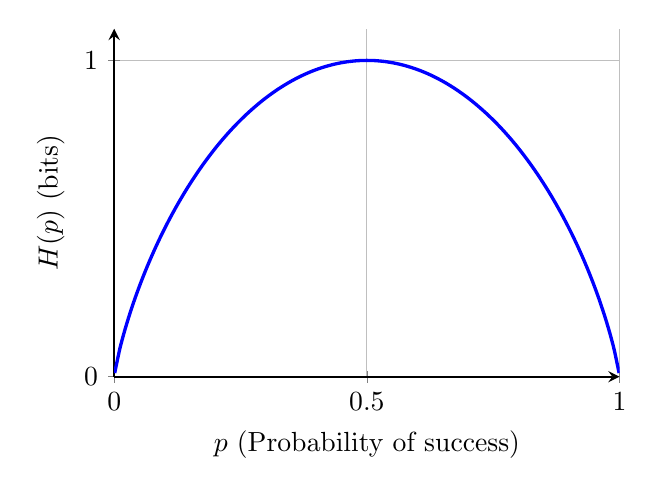
\begin{tikzpicture}
        \begin{axis}[
            width=8cm, height=6cm,
            xlabel={$p$ (Probability of success)},
            ylabel={$H(p)$ (bits)},
            xmin=0, xmax=1,
            ymin=0, ymax=1.1,
            xtick={0, 0.5, 1},
            ytick={0, 1},
            grid=major,
            axis lines=left,
            thick,
            smooth
        ]
        \addplot[domain=0.001:0.999, samples=100, blue, very thick] 
            {-x*log2(x) - (1-x)*log2(1-x)};
        \end{axis}
    \end{tikzpicture}
    \caption{The binary entropy function $H(p)$. Uncertainty is maximized when $p=0.5$ (a fair coin), yielding 1 bit of entropy.}
    \label{fig:binary_entropy}
\end{figure}

As seen in Figure~\ref{fig:binary_entropy}, entropy is maximized when the distribution is uniform (maximum uncertainty) and minimized when the distribution is deterministic (zero uncertainty).

\begin{theorem}[Maximum Entropy for Discrete Variables]
\label{thm:max_entropy}
For a discrete random variable $X$ with an alphabet size $|\mathcal{X}|$, the entropy $H(X)$ satisfies:
\begin{equation}
    0 \leq H(X) \leq \log |\mathcal{X}|
\end{equation}
The upper bound is achieved if and only if $X$ is uniformly distributed over $\mathcal{X}$.
\end{theorem}

\begin{proof}
Let $p(x)$ be the probability distribution of $X$, and let $u(x) = 1/|\mathcal{X}|$ be the uniform distribution. We use the fundamental inequality $\ln z \leq z - 1$ for $z > 0$, with equality if and only if $z = 1$.
\begin{align*}
    H(X) - \log |\mathcal{X}| &= \sum_{x} p(x) \log \frac{1}{p(x)} - \sum_{x} p(x) \log |\mathcal{X}| \\
    &= \sum_{x} p(x) \log \frac{1}{p(x)|\mathcal{X}|} \\
    &= \frac{1}{\ln 2} \sum_{x} p(x) \ln \frac{u(x)}{p(x)} \\
    &\leq \frac{1}{\ln 2} \sum_{x} p(x) \left( \frac{u(x)}{p(x)} - 1 \right) \\
    &= \frac{1}{\ln 2} \left( \sum_{x} u(x) - \sum_{x} p(x) \right) \\
    &= \frac{1}{\ln 2} (1 - 1) = 0
\end{align*}
Equality holds if and only if $u(x)/p(x) = 1$ for all $x$, meaning $p(x) = 1/|\mathcal{X}|$.
\end{proof}

\subsection{Shannon's Source Coding Theorem}

Why is $H(X)$ the fundamental limit of compression? Shannon's Source Coding Theorem establishes that $H(X)$ is the minimum expected length of any uniquely decodable binary code for $X$. 

Let $C(x)$ be the codeword for symbol $x$, and $l(x)$ be its length in bits. The expected length of the code is $L = \sum_x p(x) l(x)$.

\begin{theorem}[Shannon's Source Coding Theorem (Noiseless)]
\label{thm:source_coding}
For any uniquely decodable code representing a discrete random variable $X$, the expected length $L$ is bounded by:
\begin{equation}
    L \geq H(X)
\end{equation}
Furthermore, there exists a prefix code such that $L < H(X) + 1$.
\end{theorem}
The proof relies on the Kraft-McMillan inequality ($\sum_x 2^{-l(x)} \leq 1$), which dictates the lengths of prefix-free codes \cite{cover1999elements}.

\subsection{Worked Numerical Example}

Consider a simple weather prediction model that categorizes the next day into four states $\mathcal{X} = \{\text{Sunny, Cloudy, Rainy, Snowy}\}$ with probabilities $p = \{0.5, 0.25, 0.125, 0.125\}$.

First, we compute the Shannon entropy $H(X)$:
\begin{align*}
    H(X) &= - \left( 0.5 \log_2 0.5 + 0.25 \log_2 0.25 + 0.125 \log_2 0.125 + 0.125 \log_2 0.125 \right) \\
    &= 0.5(1) + 0.25(2) + 0.125(3) + 0.125(3) \\
    &= 0.5 + 0.5 + 0.375 + 0.375 \\
    &= 1.75 \text{ bits}
\end{align*}

To achieve a code length that matches this theoretical minimum, we can construct a Huffman tree (Figure~\ref{fig:huffman}). We assign shorter codewords to more frequent events.

\begin{figure}[ht]
    \centering
    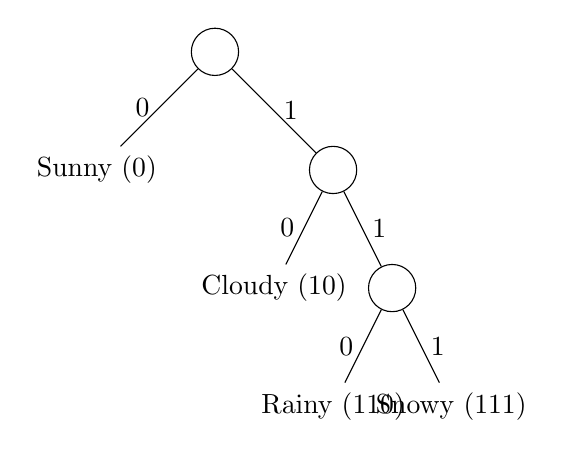
\begin{tikzpicture}[level distance=1.5cm,
      level 1/.style={sibling distance=3cm},
      level 2/.style={sibling distance=1.5cm},
      level 3/.style={sibling distance=1.5cm},
      circle node/.style={circle,draw,minimum size=6mm,inner sep=0pt}]
      
      \node[circle node] {}
        child {node {Sunny (0)} edge from parent node[left,draw=none] {0}}
        child {node[circle node] {}
          child {node {Cloudy (10)} edge from parent node[left,draw=none] {0}}
          child {node[circle node] {}
            child {node {Rainy (110)} edge from parent node[left,draw=none] {0}}
            child {node {Snowy (111)} edge from parent node[right,draw=none] {1}}
            edge from parent node[right,draw=none] {1}
          }
          edge from parent node[right,draw=none] {1}
        };
    \end{tikzpicture}
    \caption{Huffman tree for the weather prediction example. The expected code length $L = 0.5(1) + 0.25(2) + 0.125(3) + 0.125(3) = 1.75$ bits, perfectly matching $H(X)$.}
    \label{fig:huffman}
\end{figure}

In this ideal scenario, the expected code length $L$ exactly equals $H(X)$, because all probabilities are negative powers of 2. In deep learning, neural networks essentially perform a continuous version of this coding, mapping dense raw inputs into compressed latent codes $z$. 

\begin{horizon}
While Shannon's theorems strictly govern discrete, stationary distributions, the data processed by deep neural networks is often continuous, non-stationary, and intrinsically high-dimensional. Classical entropy assumes a known probability distribution $P$, but a neural network $f_\theta$ only ever sees empirical samples from a finite dataset $\mathcal{D}$. 

It is conjectured that for highly overparameterized models, the implicit regularization of stochastic gradient descent operates by minimizing a localized, empirical form of entropy over the parameter manifold. Under this view, the network does not merely compress the input; it actively reshapes the alphabet $\mathcal{X}$ into an internal latent geometry $\mathcal{Z}$ where the source coding bounds are continuously re-negotiated during training. 

An open question is whether the fundamental limits of the Source Coding Theorem can be meaningfully translated into a "Representation Coding Theorem" for intermediate layers of deep networks. If the latent space dynamically adapts, what serves as the true capacity limit? Future work in the intersection of information bottleneck theory and learning dynamics might reveal that neural networks naturally converge to solutions that are optimal not just for generalization, but for thermodynamic efficiency.
\end{horizon}

\section*{Summary}
In this chapter, we introduced the foundational currency of information theory: surprisal. By averaging surprisal across a probability distribution, we defined Shannon entropy $H(X)$, which quantifies the average uncertainty of a random variable. We proved that uniform distributions maximize entropy, establishing a ceiling on uncertainty. Through Shannon's Source Coding Theorem, we demonstrated that $H(X)$ represents the absolute theoretical limit for lossless data compression, setting the stage for how neural networks compress and encode representations.

\section*{Exercises}
\begin{enumerate}
    \item \textbf{Calculating Entropy:} Let $X$ represent the roll of a loaded six-sided die where $p(1)=p(2)=p(3)=p(4)=1/8$ and $p(5)=p(6)=1/4$. Calculate the Shannon entropy $H(X)$ in bits.
    \item \textbf{Binary Source:} A source produces a binary sequence of $1$s and $0$s. The probability of a $1$ is $p$. Plot the entropy $H(p)$ and find the value of $p$ that maximizes it using calculus.
    \item \textbf{Infinite Alphabet:} Consider a geometric random variable $X$ with probability mass function $p(k) = (1-p)^{k-1}p$ for $k = 1, 2, 3, \dots$. Derive a closed-form expression for the entropy $H(X)$. 
    \item \textbf{Network Weights:} Suppose a highly quantized neural network has $10^6$ parameters, each taking one of three values $\{-1, 0, 1\}$ with probabilities $\{0.2, 0.6, 0.2\}$. What is the minimum theoretical file size (in bytes) required to store these weights losslessly?
    \item \textbf{Empirical vs True Entropy:} Discuss the difficulty of estimating the entropy of an image dataset (e.g., $256 \times 256$ RGB images) directly from its empirical distribution $\mathcal{D}$. Why does the plug-in estimator $\hat{H} = -\sum \hat{p}(x)\log \hat{p}(x)$ fail catastrophically in this high-dimensional regime?
\end{enumerate}

\chapter{Joint and Conditional Entropy}
\label{ch:joint_conditional}

\section{The Geometry of Intersecting Uncertainties}

If the previous chapter dealt with the uncertainty of a single isolated event, this chapter deals with the reality of the physical world: events are almost never isolated. The sky being cloudy is not independent of whether it will rain. The pixel in the upper-left corner of an image is not independent of the pixel next to it. The entire premise of machine learning is built upon exploiting these dependencies. If variables were truly independent, prediction would be impossible.

To build neural networks that can predict $\mathcal{Y}$ from $\mathcal{X}$, we must first understand how to measure the joint uncertainty of multiple variables, and crucially, how the knowledge of one variable reduces the uncertainty of another. This brings us to the concepts of joint entropy and conditional entropy. 

Imagine two random variables as two overlapping shadows cast on a wall. The total area covered by both shadows represents their joint entropy---the total uncertainty when considering both variables together. The area where they overlap represents the information they share. The area of one shadow that is not covered by the other represents the conditional entropy---the remaining uncertainty in one variable after the other is fully known. 

In deep learning, this geometry of intersecting uncertainties is what we navigate during training. When an encoder network $q_\phi(z|x)$ maps an input $x$ to a latent representation $z$, we are acutely interested in the conditional entropy $H(Z|X)$. If the encoder is deterministic, this conditional entropy is zero. If it is stochastic, as in Variational Autoencoders, this conditional entropy represents the noise injected into the representation. Understanding how uncertainties combine and condition one another is the prerequisite for understanding mutual information, which we will tackle in the next chapter.

\section{Mathematical Definitions}

We begin by extending our definition of entropy to multiple variables. Let $X$ and $Y$ be discrete random variables drawn from alphabets $\mathcal{X}$ and $\mathcal{Y}$, respectively, with a joint probability mass function $p(x, y) = \text{Pr}(X=x, Y=y)$.

\begin{definition}[Joint Entropy]
The joint entropy $H(X, Y)$ of a pair of discrete random variables $(X, Y)$ is defined as the expected surprisal of their joint outcomes:
\begin{equation}
    H(X, Y) = -\sum_{x \in \mathcal{X}} \sum_{y \in \mathcal{Y}} p(x, y) \log p(x, y)
\end{equation}
\end{definition}

Joint entropy measures the total uncertainty needed to describe both $X$ and $Y$ simultaneously. It is straightforward to see that if $X$ and $Y$ are completely independent, meaning $p(x, y) = p(x)p(y)$ for all $x$ and $y$, then the logarithm splits, and $H(X, Y) = H(X) + H(Y)$. The uncertainties simply add up.

However, when variables are dependent, knowing one tells us something about the other. This remaining uncertainty is formalized as conditional entropy.

\begin{definition}[Conditional Entropy]
The conditional entropy $H(Y|X)$ of a random variable $Y$ given another random variable $X$ is the expected value of the entropies of the conditional distributions $p(y|x)$, averaged over the distribution of $x$:
\begin{equation}
    H(Y|X) = \sum_{x \in \mathcal{X}} p(x) H(Y | X=x) = -\sum_{x \in \mathcal{X}} \sum_{y \in \mathcal{Y}} p(x, y) \log p(y|x)
\end{equation}
\end{definition}

This definition is crucial. It answers the question: ``If I already know $X$, how much uncertainty still remains about $Y$ on average?'' 

\begin{theorem}[Chain Rule of Entropy]
\label{thm:chain_rule}
The joint entropy of $X$ and $Y$ is the entropy of $X$ plus the conditional entropy of $Y$ given $X$:
\begin{equation}
    H(X, Y) = H(X) + H(Y|X)
\end{equation}
\end{theorem}

\begin{proof}
By the definition of conditional probability, $p(x, y) = p(x)p(y|x)$. Substituting this into the definition of joint entropy:
\begin{align*}
    H(X, Y) &= -\sum_{x \in \mathcal{X}} \sum_{y \in \mathcal{Y}} p(x, y) \log p(x, y) \\
    &= -\sum_{x \in \mathcal{X}} \sum_{y \in \mathcal{Y}} p(x, y) \log \left( p(x) p(y|x) \right) \\
    &= -\sum_{x \in \mathcal{X}} \sum_{y \in \mathcal{Y}} p(x, y) \log p(x) - \sum_{x \in \mathcal{X}} \sum_{y \in \mathcal{Y}} p(x, y) \log p(y|x) \\
    &= -\sum_{x \in \mathcal{X}} p(x) \log p(x) \underbrace{\sum_{y \in \mathcal{Y}} p(y|x)}_{1} + H(Y|X) \\
    &= H(X) + H(Y|X)
\end{align*}
The proof demonstrates how total uncertainty is built sequentially.
\end{proof}

\begin{corollary}[Conditioning Reduces Entropy]
For any two random variables $X$ and $Y$:
\begin{equation}
    H(Y|X) \leq H(Y)
\end{equation}
with equality if and only if $X$ and $Y$ are independent.
\end{corollary}
This confirms our intuition: knowing $X$ can only ever decrease (or leave unchanged) our uncertainty about $Y$. It can never increase it. Information is always non-negative.

\subsection{Worked Numerical Example}

Consider a dataset $\mathcal{D}$ where instances are either cats or dogs (variable $Y$), and they wear collars or do not (variable $X$). The joint distribution $p(x, y)$ is given by the following table:

\begin{center}
\begin{tabular}{c|cc|c}
 & $Y = \text{Dog}$ & $Y = \text{Cat}$ & Marginal $p(x)$ \\
\hline
$X = \text{Collar}$ & 0.4 & 0.1 & 0.5 \\
$X = \text{No Collar}$ & 0.2 & 0.3 & 0.5 \\
\hline
Marginal $p(y)$ & 0.6 & 0.4 & 1.0
\end{tabular}
\end{center}

First, let's calculate the marginal entropies $H(X)$ and $H(Y)$:
\begin{align*}
    H(X) &= - (0.5 \log_2 0.5 + 0.5 \log_2 0.5) = 1 \text{ bit} \\
    H(Y) &= - (0.6 \log_2 0.6 + 0.4 \log_2 0.4) \approx 0.971 \text{ bits}
\end{align*}

Next, the joint entropy $H(X, Y)$:
\begin{align*}
    H(X, Y) &= - (0.4 \log_2 0.4 + 0.1 \log_2 0.1 + 0.2 \log_2 0.2 + 0.3 \log_2 0.3) \\
    &\approx 0.529 + 0.332 + 0.464 + 0.521 = 1.846 \text{ bits}
\end{align*}

Now, let's calculate the conditional entropy $H(Y|X)$. We need the conditional distributions $p(y|x) = p(x, y)/p(x)$:
For $X = \text{Collar}$: $p(\text{Dog}|\text{Collar}) = 0.4/0.5 = 0.8$, $p(\text{Cat}|\text{Collar}) = 0.2$.
For $X = \text{No Collar}$: $p(\text{Dog}|\text{No Collar}) = 0.2/0.5 = 0.4$, $p(\text{Cat}|\text{No Collar}) = 0.6$.

\begin{align*}
    H(Y|X=\text{Collar}) &= - (0.8 \log_2 0.8 + 0.2 \log_2 0.2) \approx 0.722 \text{ bits} \\
    H(Y|X=\text{No Collar}) &= - (0.4 \log_2 0.4 + 0.6 \log_2 0.6) \approx 0.971 \text{ bits}
\end{align*}

Averaging these over $p(x)$:
\begin{align*}
    H(Y|X) &= 0.5 \times 0.722 + 0.5 \times 0.971 \\
    &= 0.361 + 0.4855 = 0.8465 \text{ bits}
\end{align*}

We can verify the chain rule: $H(X) + H(Y|X) = 1 + 0.8465 = 1.8465 \approx H(X, Y)$.
Notice that $H(Y|X) = 0.8465 < H(Y) = 0.971$. Knowing whether the animal has a collar reduces our uncertainty about whether it is a dog or a cat.

\begin{figure}[ht]
    \centering
    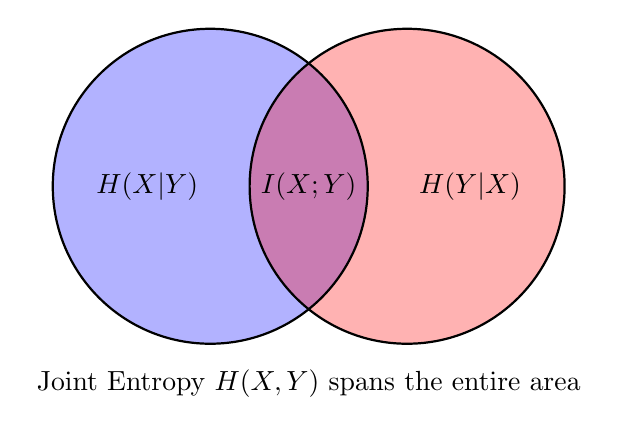
\begin{tikzpicture}
      % Left circle (X)
      \fill[blue, opacity=0.3] (0,0) circle (2cm);
      % Right circle (Y)
      \fill[red, opacity=0.3] (2.5,0) circle (2cm);
      
      % Outlines
      \draw[thick] (0,0) circle (2cm);
      \draw[thick] (2.5,0) circle (2cm);
      
      % Labels
      \node at (-0.8, 0) {$H(X|Y)$};
      \node at (3.3, 0) {$H(Y|X)$};
      \node at (1.25, 0) {$I(X;Y)$};
      
      % Overall label
      \node at (1.25, -2.5) {Joint Entropy $H(X,Y)$ spans the entire area};
    \end{tikzpicture}
    \caption{Information Venn Diagram. The total area represents the joint entropy $H(X,Y)$. The non-overlapping regions are the conditional entropies, while the intersection is the mutual information.}
    \label{fig:venn}
\end{figure}

\begin{figure}[ht]
    \centering
    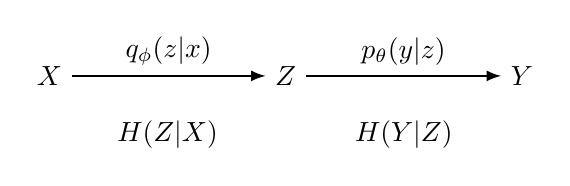
\begin{tikzpicture}[>=latex, scale=1.5]
        % Nodes
        \node (x) at (0, 0) {$X$};
        \node (z) at (2, 0) {$Z$};
        \node (y) at (4, 0) {$Y$};
        
        % Arrows
        \draw[->, thick] (x) -- (z) node[midway, above] {$q_\phi(z|x)$};
        \draw[->, thick] (z) -- (y) node[midway, above] {$p_\theta(y|z)$};
        
        % Annotations
        \node at (1, -0.5) {$H(Z|X)$};
        \node at (3, -0.5) {$H(Y|Z)$};
    \end{tikzpicture}
    \caption{A Markov chain in a typical representation learning setup. The conditional entropy $H(Z|X)$ dictates the stochasticity of the encoder.}
    \label{fig:markov_encoder}
\end{figure}

In the context of deep learning (Figure~\ref{fig:markov_encoder}), when we feed data $x$ into a neural network to produce a representation $z$, we are defining a conditional distribution $q_\phi(z|x)$. If this mapping is a standard deterministic feedforward network, then $p(z|x) = 1$ for the specific output and $0$ otherwise. Consequently, the conditional entropy $H(Z|X) = 0$. However, in models like Variational Autoencoders \cite{kingma2013auto}, the encoder maps to a Gaussian distribution, making $H(Z|X) > 0$. This non-zero conditional entropy acts as a regularizer, forcing the network to smooth its representations and preventing it from memorizing the exact input $x$.

\begin{horizon}
The mathematical bedrock of conditional entropy is universally accepted for discrete and well-behaved continuous distributions. However, deep neural networks routinely process highly dimensional data where the true joint distribution $P_{\text{data}}(X,Y)$ is unknown and arguably uncomputable. 

It is conjectured that the implicit bias of optimization algorithms like SGD biases networks toward representations $Z$ that minimize the conditional entropy $H(Y|Z)$ (maximizing predictive accuracy) while simultaneously, and perhaps inadvertently, increasing $H(Z|X)$ by flattening local minima in the parameter space. This suggests a thermodynamic tradeoff between the precision of the output and the ``heat'' or noise tolerated in the internal representation.

An open question is how to rigorously quantify $H(Z|X)$ when $f_\theta$ is formally deterministic (hence $H(Z|X)=0$ in Shannon's sense), but highly sensitive to imperceptible input noise, as seen in adversarial examples. Can conditional entropy be redefined topologically or geometrically on the data manifold to reflect this practical fragility? Future research into information geometry might bridge this gap by treating adversarial robustness as a constraint on the empirical conditional entropy.
\end{horizon}

\section*{Summary}
In this chapter, we expanded our view from single variables to interacting systems. Joint entropy $H(X,Y)$ quantifies the total uncertainty of a system, while conditional entropy $H(Y|X)$ measures the remaining uncertainty in $Y$ when $X$ is known. We proved the Chain Rule of Entropy, demonstrating how uncertainties aggregate. Finally, we saw how conditional entropy acts as a measure of stochasticity in neural network encoders, serving as a critical control knob in generative modeling.

\section*{Exercises}
\begin{enumerate}
    \item \textbf{Symmetry:} Prove that $H(X,Y) = H(Y,X)$ and interpret this result. Does $H(X|Y) = H(Y|X)$? Give a counterexample if false.
    \item \textbf{Deterministic Functions:} If $Y = f(X)$ where $f$ is a deterministic function, prove that $H(Y|X) = 0$. Then prove that $H(X,Y) = H(X)$.
    \item \textbf{Chain Rule for N Variables:} Extend Theorem~\ref{thm:chain_rule} to three variables, expressing $H(X,Y,Z)$ in terms of individual conditional entropies.
    \item \textbf{Network Encoders:} Let $x$ be an image and $z = q_\phi(x)$ be a latent vector. If $q_\phi$ adds isotropic Gaussian noise $\mathcal{N}(0, \sigma^2 I)$ to the output, write an expression for $H(Z|X)$. How does $\sigma$ affect the model's capacity to memorize $x$?
    \item \textbf{Data Processing:} If $X \to Y \to Z$ form a Markov chain, prove that $H(Z|X) \leq H(Z|Y)$ is generally false. Construct a counterexample.
\end{enumerate}

\chapter{Mutual Information and the Data Processing Inequality}
\label{ch:mutual_information}

\section{The Currency of Representation}

If entropy is the measure of uncertainty, mutual information is the measure of insight. When a neural network processes an image to classify a breed of dog, we do not care about the entropy of the hidden layers in isolation. We care about how much those hidden layers actually know about the target label. Mutual information is the mathematical formalized answer to the question: ``How much does knowing $X$ reduce my uncertainty about $Y$?''

In deep learning, mutual information is arguably the most critical quantity. It serves as the primary currency exchanged during representation learning. Contrastive learning methods like SimCLR and InfoNCE are, at their core, algorithms designed to maximize the mutual information between different augmentations of the same image. The Information Bottleneck principle frames deep learning entirely as an optimization of mutual information: maximizing the mutual information between the representation and the label, while minimizing the mutual information between the representation and the raw input. 

Yet, there is a strict, physical constraint on this currency. Information cannot be spontaneously generated by processing data. A deterministic function applied to a signal can only destroy information or preserve it; it can never add new information about the original source. This profound truth is known as the Data Processing Inequality (DPI). The DPI governs the forward pass of every neural network. As data flows from the input layer through the hidden layers to the output, the mutual information with the target label monotonically decreases (or stays flat). The magic of deep learning is not in creating information, but in stripping away the irrelevant noise so that the remaining information is linearly separable.

\section{Mathematical Definitions}

Building upon the definitions of entropy and conditional entropy from previous chapters, we formally define mutual information.

\begin{definition}[Mutual Information]
The mutual information $I(X; Y)$ between two discrete random variables $X$ and $Y$ is the reduction in uncertainty of $X$ due to the knowledge of $Y$:
\begin{equation}
    I(X; Y) = H(X) - H(X|Y)
\end{equation}
\end{definition}

Because of the symmetry of joint entropy ($H(X,Y) = H(Y,X)$), we can rewrite this in several insightful ways:
\begin{align}
    I(X; Y) &= H(Y) - H(Y|X) \label{eq:mi_sym1} \\
    I(X; Y) &= H(X) + H(Y) - H(X, Y) \label{eq:mi_sym2} \\
    I(X; Y) &= \sum_{x \in \mathcal{X}} \sum_{y \in \mathcal{Y}} p(x, y) \log \frac{p(x, y)}{p(x)p(y)} \label{eq:mi_kl}
\end{align}

Equation~\ref{eq:mi_kl} reveals a deep connection: mutual information is the Kullback-Leibler (KL) divergence between the joint distribution $p(x,y)$ and the product of the marginal distributions $p(x)p(y)$. It measures how far the variables are from being strictly independent.

\begin{theorem}[Non-negativity of Mutual Information]
For any two random variables $X$ and $Y$, $I(X;Y) \geq 0$, with equality if and only if $X$ and $Y$ are independent.
\end{theorem}
\begin{proof}
By definition, $I(X;Y) = H(X) - H(X|Y)$. Since conditioning reduces entropy (Corollary from Chapter~\ref{ch:joint_conditional}), $H(X|Y) \leq H(X)$, implying $I(X;Y) \geq 0$. Equality holds if $H(X|Y) = H(X)$, meaning knowledge of $Y$ does not change the distribution of $X$, which is the definition of independence.
\end{proof}

\subsection{The Data Processing Inequality}

To discuss the flow of information through a neural network, we must define a Markov chain. Random variables $X$, $Y$, and $Z$ form a Markov chain $X \to Y \to Z$ if the conditional distribution of $Z$ depends only on $Y$ and is conditionally independent of $X$. Mathematically: $p(z|x,y) = p(z|y)$. 

In deep learning, the sequence of layers $X \to H_1 \to H_2 \to \dots \to \hat{Y}$ strictly forms a Markov chain.

\begin{theorem}[Data Processing Inequality]
\label{thm:dpi}
If $X \to Y \to Z$ forms a Markov chain, then the mutual information cannot increase:
\begin{equation}
    I(X; Y) \geq I(X; Z)
\end{equation}
\end{theorem}

\begin{proof}
By the chain rule for mutual information, we can expand $I(X; Y, Z)$ in two different ways:
\begin{align}
    I(X; Y, Z) &= I(X; Z) + I(X; Y | Z) \label{eq:dpi1} \\
    I(X; Y, Z) &= I(X; Y) + I(X; Z | Y) \label{eq:dpi2}
\end{align}
Since $X \to Y \to Z$ is a Markov chain, $X$ and $Z$ are conditionally independent given $Y$. Therefore, $I(X; Z | Y) = 0$.
Substituting this into Equation~\ref{eq:dpi2} gives $I(X; Y, Z) = I(X; Y)$.
Equating this with Equation~\ref{eq:dpi1}:
\begin{equation}
    I(X; Y) = I(X; Z) + I(X; Y | Z)
\end{equation}
Since mutual information is always non-negative, $I(X; Y | Z) \geq 0$, which requires that:
\begin{equation}
    I(X; Y) \geq I(X; Z)
\end{equation}
\end{proof}

\begin{figure}[ht]
    \centering
    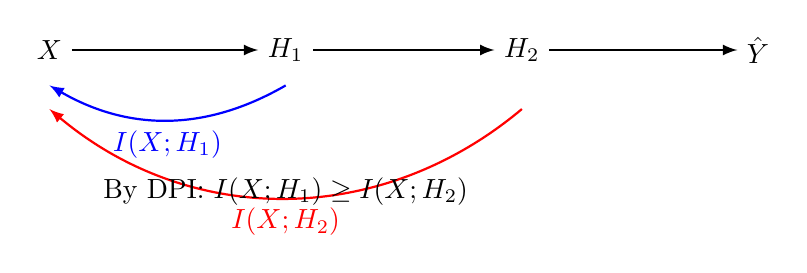
\begin{tikzpicture}[>=latex, scale=1.5]
        \node (x) at (0, 0) {$X$};
        \node (h1) at (2, 0) {$H_1$};
        \node (h2) at (4, 0) {$H_2$};
        \node (y) at (6, 0) {$\hat{Y}$};
        
        \draw[->, thick] (x) -- (h1);
        \draw[->, thick] (h1) -- (h2);
        \draw[->, thick] (h2) -- (y);
        
        \draw[<-, thick, blue, bend right=30] (0, -0.3) to node[below] {$I(X;H_1)$} (2, -0.3);
        \draw[<-, thick, red, bend right=40] (0, -0.5) to node[below] {$I(X;H_2)$} (4, -0.5);
        
        \node at (2, -1.2) {By DPI: $I(X;H_1) \geq I(X;H_2)$};
    \end{tikzpicture}
    \caption{Information flow through the layers of a neural network. Information about the input $X$ can only degrade as it moves deeper into the network.}
    \label{fig:dpi_network}
\end{figure}

The DPI (Figure~\ref{fig:dpi_network}) implies that no clever manipulation of $Y$ can uncover more information about $X$ than was originally present in $Y$. 

\subsection{Worked Numerical Example}

Suppose a binary input signal $X \in \{0,1\}$ is transmitted through two noisy channels in sequence to produce $Y$ and then $Z$. 
Let $p(x=0) = 0.5$ and $p(x=1) = 0.5$.
The first channel flips the bit with probability $p=0.1$. Thus, $p(y \neq x) = 0.1$.
The second channel flips the bit again with probability $q=0.2$. Thus, $p(z \neq y) = 0.2$.

First, let's find $I(X; Y)$. 
$H(X) = 1$ bit. 
The conditional entropy $H(X|Y)$ depends on the error rate of the channel. Since it's a symmetric binary channel with crossover probability 0.1, $H(X|Y) = H(0.1) = -0.1\log_2 0.1 - 0.9\log_2 0.9 \approx 0.469$ bits.
\begin{equation*}
    I(X; Y) = H(X) - H(X|Y) = 1 - 0.469 = 0.531 \text{ bits.}
\end{equation*}

Now, what is $I(X; Z)$? 
The total probability of a bit flip from $X$ to $Z$ happens if the first channel flips it and the second doesn't, OR the first doesn't and the second does.
$P(Z \neq X) = (0.1)(0.8) + (0.9)(0.2) = 0.08 + 0.18 = 0.26$.
So the effective channel from $X$ to $Z$ has an error rate of 0.26.
$H(X|Z) = H(0.26) = -0.26\log_2 0.26 - 0.74\log_2 0.74 \approx 0.827$ bits.
\begin{equation*}
    I(X; Z) = H(X) - H(X|Z) = 1 - 0.827 = 0.173 \text{ bits.}
\end{equation*}

As expected by the Data Processing Inequality, $I(X; Y) > I(X; Z)$ ($0.531 > 0.173$). Information is lost in transit.

\begin{figure}[ht]
    \centering
    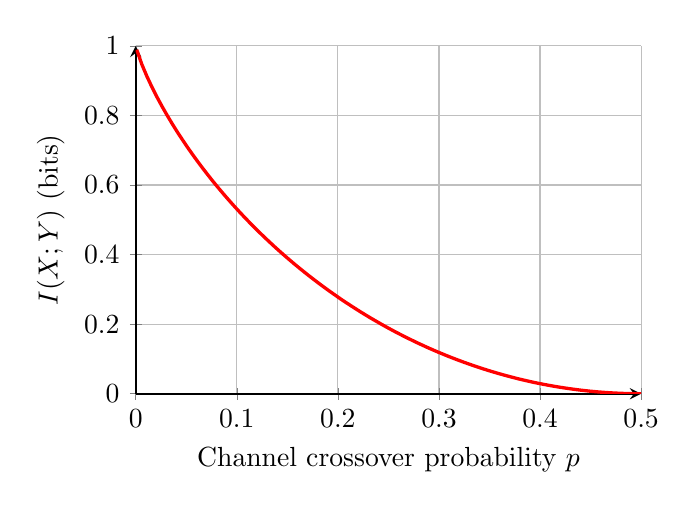
\begin{tikzpicture}[>=latex, scale=1]
        \begin{axis}[
            width=8cm, height=6cm,
            xlabel={Channel crossover probability $p$},
            ylabel={$I(X;Y)$ (bits)},
            xmin=0, xmax=0.5,
            ymin=0, ymax=1,
            grid=major,
            axis lines=left,
            thick
        ]
        \addplot[domain=0.001:0.5, samples=100, red, very thick] 
            {1 - (-x*log2(x) - (1-x)*log2(1-x))};
        \end{axis}
    \end{tikzpicture}
    \caption{Mutual information between input and output of a binary symmetric channel as a function of error rate $p$. As noise increases, mutual information drops to zero.}
    \label{fig:capacity}
\end{figure}

\begin{horizon}
The strict formulation of the Data Processing Inequality forms an ironclad bound on deep learning representations: a layer $H_n$ can never contain more information about the target label $Y$ than the previous layer $H_{n-1}$. This mathematically justifies why deep networks must focus on discarding irrelevant noise, rather than creating signal.

However, in practice, deep networks are not evaluated on raw mutual information, but on "usable" or "accessible" information. While $I(X;H_1) \geq I(X;H_n)$, the information in $H_1$ is highly entangled and non-linear, whereas the information in $H_n$ is linearly separable by a simple softmax layer. 

It is conjectured that deep learning operates by sacrificing total mutual information $I(X;Z)$ in exchange for maximizing the linearly decodable mutual information $I_{lin}(Y;Z)$. An open question is how to rigorously define this "usable" information metric. If we can bound the gap between $I(Y;Z)$ and $I_{lin}(Y;Z)$, we could theoretically predict a network's test accuracy purely by examining the geometry of its latent space, without running inference. Future work attempting to bridge classical Shannon information with Vapnik-Chervonenkis (VC) theory might yield a modified DPI that accounts for computational complexity.
\end{horizon}

\section*{Summary}
Mutual information $I(X;Y)$ measures the amount of information that one variable contains about another. It is symmetric, non-negative, and intimately related to KL divergence. Crucially, the Data Processing Inequality (DPI) establishes that post-processing cannot increase information. In a Markov chain $X \to Y \to Z$, $I(X;Y) \geq I(X;Z)$. This fundamental theorem reveals that neural networks do not synthesize new information about the target; rather, they transform existing information into a more accessible format while deliberately discarding irrelevant nuisance variables.

\section*{Exercises}
\begin{enumerate}
    \item \textbf{Venn Diagram Proofs:} Using the definitions of $H(X)$, $H(X,Y)$, and $H(X|Y)$, prove that $I(X;Y) = H(X) + H(Y) - H(X,Y)$.
    \item \textbf{Deterministic Bottleneck:} Consider an image classifier where $x \in \mathbb{R}^{784}$ (MNIST) is mapped to a bottleneck $z \in \mathbb{R}^{2}$, and then to a prediction $\hat{y}$. Why must the classification accuracy be bounded by the mutual information capacity of the 2D bottleneck? 
    \item \textbf{Sufficient Statistics:} A statistic $T(X)$ is called a sufficient statistic for a parameter $\theta$ if $I(\theta; X) = I(\theta; T(X))$. Show that if $T(X)$ is sufficient, the DPI holds with equality in the chain $\theta \to X \to T(X)$. 
    \item \textbf{Mutual Information of Continuous Variables:} Why does $I(X;Y)$ remain perfectly well-defined and positive for continuous variables, even though differential entropy $h(X)$ can be negative?
\end{enumerate}

% TODO-CITE: Ensure all named results are cited.

\chapter{Divergence, Cross-Entropy, and Metric Spaces}

\section{The Geometry of Belief}
Machine learning, at its core, is an exercise in approximation. We are granted access to a limited set of observations drawn from an unknown, underlying reality, and we are tasked with constructing a surrogate model that mimics this reality as closely as possible. In the language of probability, we are given samples from a true data distribution $P$, and we seek a model distribution $Q$ that approximates $P$. But what does it mean for two distributions to be ``close''?

In physical space, distance is unambiguous. The distance between two cities can be measured with a ruler and obeys intuitive geometric rules: it is symmetric (the distance from $A$ to $B$ is the distance from $B$ to $A$), and it satisfies the triangle inequality (the detour through $C$ cannot be shorter than the straight line from $A$ to $B$). Spaces equipped with such a distance function are called metric spaces.

However, the space of probability distributions---often termed the statistical manifold---does not naturally yield to the geometry of physical space. When we modify our beliefs or update a model's parameters, we are traversing this space, and the ``distance'' we measure is fundamentally tied to information, not physical length. The cost of replacing the true distribution $P$ with an approximation $Q$ is best understood through the lens of encoding and surprisal.

This brings us to the concept of Cross-Entropy and the Kullback-Leibler (KL) divergence. Cross-entropy measures the total expected cost of encoding events from $P$ using a coding scheme optimized for $Q$. The KL divergence represents the \textit{excess} cost, the penalty incurred precisely because $Q$ is not $P$. Unlike physical distance, information divergence is inherently asymmetric. It is far more penalizing to assign zero probability to an event that actually occurs than to assign positive probability to an event that never occurs. This asymmetry reflects the directional nature of learning and approximation: the model $Q$ must conform to the reality $P$, not the other way around.

As we delve into the mathematical formulations of these concepts, we must abandon our reliance on simple Euclidean intuition. We will see that while KL divergence lacks the properties of a true metric, it provides a profoundly meaningful measure of informational discrepancy. We will also explore how to bridge the gap between information divergence and true metric spaces, paving the way for advanced tools in deep learning.

\section{Mathematical Foundations of Divergence}

To quantify the difference between two probability distributions, we begin with Cross-Entropy.

\begin{definition}[Cross-Entropy]
Let $P$ and $Q$ be two probability distributions defined over the same discrete support $\mathcal{X}$. The cross-entropy $H(P, Q)$ is defined as the expected surprisal of events from $P$ when evaluated under the model $Q$:
\begin{equation}
H(P, Q) = -\sum_{x \in \mathcal{X}} P(x) \log Q(x)
\end{equation}
For continuous distributions with probability density functions $p(x)$ and $q(x)$, the cross-entropy is:
\begin{equation}
H(P, Q) = -\int_{\mathcal{X}} p(x) \log q(x) \, dx
\end{equation}
\end{definition}

Cross-entropy is the standard objective function in classification tasks within deep learning, where $P$ represents the empirical distribution (one-hot labels) and $Q$ is the network's predicted softmax distribution.

The cross-entropy can be decomposed into the entropy of the true distribution $P$ and the Kullback-Leibler divergence from $P$ to $Q$.

\begin{definition}[Kullback-Leibler Divergence]
The Kullback-Leibler (KL) divergence, or relative entropy, from $P$ to $Q$ is defined as:
\begin{equation}
D_{\text{KL}}(P \parallel Q) = \sum_{x \in \mathcal{X}} P(x) \log \frac{P(x)}{Q(x)}
\end{equation}
\end{definition}

\begin{theorem}[Cross-Entropy Decomposition]
For any two distributions $P$ and $Q$ over $\mathcal{X}$,
\begin{equation}
H(P, Q) = H(P) + D_{\text{KL}}(P \parallel Q)
\end{equation}
\end{theorem}
\begin{proof}
By direct substitution of the definitions:
\begin{align*}
H(P, Q) &= -\sum_{x \in \mathcal{X}} P(x) \log Q(x) \\
&= -\sum_{x \in \mathcal{X}} P(x) \log Q(x) + \sum_{x \in \mathcal{X}} P(x) \log P(x) - \sum_{x \in \mathcal{X}} P(x) \log P(x) \\
&= -\sum_{x \in \mathcal{X}} P(x) \log P(x) + \sum_{x \in \mathcal{X}} P(x) \left( \log P(x) - \log Q(x) \right) \\
&= H(P) + \sum_{x \in \mathcal{X}} P(x) \log \frac{P(x)}{Q(x)} \\
&= H(P) + D_{\text{KL}}(P \parallel Q)
\end{align*}
Since $H(P)$ depends solely on the data distribution and is fixed with respect to model parameters, minimizing the cross-entropy $H(P, Q)$ is strictly equivalent to minimizing the KL divergence $D_{\text{KL}}(P \parallel Q)$.
\end{proof}

A foundational property of the KL divergence is that it is non-negative, formalizing the intuition that any approximation $Q$ can only be sub-optimal or perfectly equal to $P$. This is established by Gibbs' Inequality.

\begin{theorem}[Gibbs' Inequality]
For any two probability distributions $P$ and $Q$, $D_{\text{KL}}(P \parallel Q) \ge 0$. Furthermore, $D_{\text{KL}}(P \parallel Q) = 0$ if and only if $P(x) = Q(x)$ for all $x \in \mathcal{X}$ almost everywhere.
\end{theorem}
\begin{proof}
We employ Jensen's Inequality, which states that for any strictly convex function $f$ and non-degenerate random variable $Z$, $\mathbb{E}[f(Z)] \ge f(\mathbb{E}[Z])$. The function $f(t) = -\log(t)$ is strictly convex on $(0, \infty)$.
\begin{align*}
D_{\text{KL}}(P \parallel Q) &= \sum_{x \in \mathcal{X}} P(x) \log \frac{P(x)}{Q(x)} \\
&= \sum_{x \in \mathcal{X}} P(x) \left( -\log \frac{Q(x)}{P(x)} \right) \\
&= \mathbb{E}_{X \sim P}\left[ -\log \frac{Q(X)}{P(X)} \right]
\end{align*}
Applying Jensen's Inequality:
\begin{align*}
\mathbb{E}_{X \sim P}\left[ -\log \frac{Q(X)}{P(X)} \right] &\ge -\log \left( \mathbb{E}_{X \sim P}\left[ \frac{Q(X)}{P(X)} \right] \right) \\
&= -\log \left( \sum_{x \in \mathcal{X}} P(x) \frac{Q(x)}{P(x)} \right) \\
&= -\log \left( \sum_{x \in \mathcal{X}} Q(x) \right)
\end{align*}
Since $Q$ is a valid probability distribution, its sum over the support must be less than or equal to $1$ (equal to $1$ if the support of $Q$ perfectly contains the support of $P$). Thus, $\sum_x Q(x) \le 1$. Since $-\log$ is a monotonically decreasing function, it follows that:
\begin{equation*}
D_{\text{KL}}(P \parallel Q) \ge -\log(1) = 0
\end{equation*}
Because $f(t) = -\log(t)$ is strictly convex, equality holds if and only if the random variable $\frac{Q(X)}{P(X)}$ is a constant with probability $1$. Given that both $P$ and $Q$ integrate to $1$, this constant must be $1$, implying $P(x) = Q(x)$ almost everywhere.
\end{proof}

\begin{figure}[htbp]
\centering
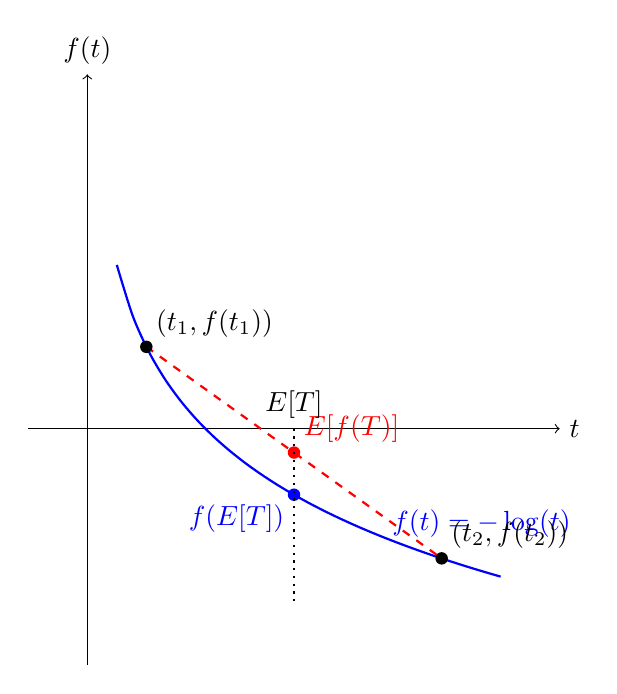
\begin{tikzpicture}[scale=1.5]
  % Draw axes
  \draw[->] (-0.5, 0) -- (4, 0) node[right] {$t$};
  \draw[->] (0, -2) -- (0, 3) node[above] {$f(t)$};
  
  % Draw strictly convex function -log(t)
  \draw[domain=0.25:3.5, smooth, variable=\t, blue, thick] plot ({\t}, {-ln(\t)});
  \node[blue, right] at (2.5, -0.8) {$f(t) = -\log(t)$};
  
  % Draw points and secant line
  \coordinate (A) at (0.5, 0.693);
  \coordinate (B) at (3, -1.098);
  
  \draw[red, dashed, thick] (A) -- (B);
  
  \fill[black] (A) circle (1.5pt) node[above right] {$(t_1, f(t_1))$};
  \fill[black] (B) circle (1.5pt) node[above right] {$(t_2, f(t_2))$};
  
  \coordinate (C) at (1.75, -0.202); % Midpoint on secant line
  \fill[red] (C) circle (1.5pt) node[above right, text=red] {$\mathbb{E}[f(T)]$};
  
  \coordinate (D) at (1.75, -0.559); % Value on function curve
  \fill[blue] (D) circle (1.5pt) node[below left, text=blue] {$f(\mathbb{E}[T])$};
  
  \draw[dotted, thick] (1.75, 0) node[above] {$\mathbb{E}[T]$} -- (1.75, -1.5);
\end{tikzpicture}
\caption{An illustration of Jensen's Inequality for the strictly convex function $f(t) = -\log(t)$. The expected value of the function (evaluated on the red secant line) is strictly greater than or equal to the function of the expected value (on the blue curve). This geometric property is the foundation for proving that $D_{\text{KL}} \ge 0$.}
\label{fig:jensens}
\end{figure}

\subsection{Asymmetry and Mode-Seeking vs. Mean-Seeking Behavior}

The Kullback-Leibler divergence is not a true metric because it is inherently asymmetric: $D_{\text{KL}}(P \parallel Q) \ne D_{\text{KL}}(Q \parallel P)$ in the general case. Furthermore, it does not satisfy the triangle inequality. The choice of direction when minimizing KL divergence profoundly impacts the behavior of the resulting approximation $Q$.

\begin{itemize}
    \item \textbf{Forward KL} ($D_{\text{KL}}(P \parallel Q)$): This is the standard objective in deep learning (equivalent to Maximum Likelihood). The term $P(x) \log \frac{P(x)}{Q(x)}$ implies that if $P(x) > 0$, $Q(x)$ must also be strictly greater than $0$ to avoid an infinite penalty ($\log \frac{P(x)}{0} \to \infty$). Thus, $Q$ is forced to cover all regions where $P$ has mass. When $Q$ is a simpler distribution than $P$, this leads to a \textit{mean-seeking} or \textit{mass-covering} behavior.
    \item \textbf{Reverse KL} ($D_{\text{KL}}(Q \parallel P)$): This formulation is common in Variational Inference (e.g., maximizing the ELBO). Here, the term is $Q(x) \log \frac{Q(x)}{P(x)}$. If $P(x) = 0$, $Q(x)$ must be exactly $0$ to avoid an infinite penalty. The model $Q$ will strongly tend to place mass only where $P$ has high mass, aggressively avoiding regions where $P$ is low. This leads to \textit{mode-seeking} behavior, where $Q$ often captures a single mode of a multimodal $P$, heavily underestimating the true variance.
\end{itemize}

\begin{figure}[htbp]
\centering
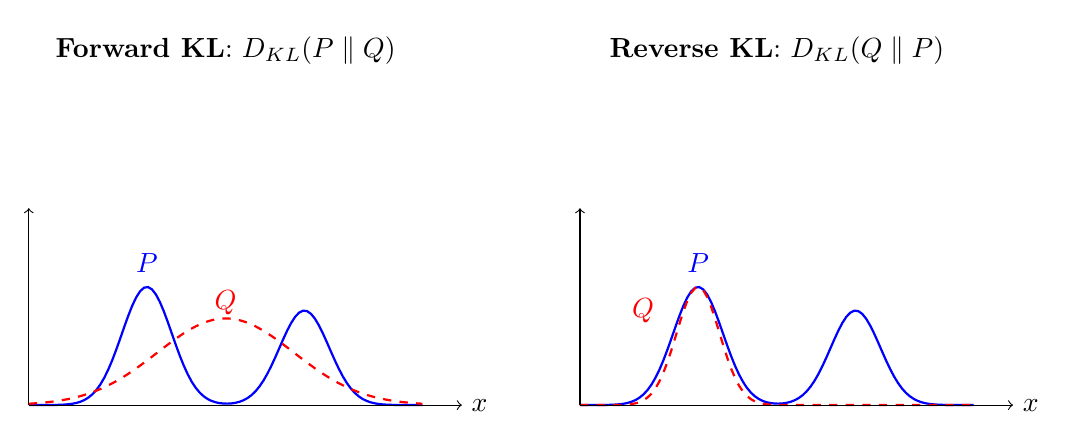
\begin{tikzpicture}[scale=1]
  % Forward KL (Mean-Seeking)
  \begin{scope}[xshift=0cm]
    \node at (2.5, 4.5) {\textbf{Forward KL}: $D_{\text{KL}}(P \parallel Q)$};
    % P(x) bimodal
    \draw[blue, thick, domain=0:5, samples=100] plot (\x, {1.5*exp(-(\x-1.5)^2/0.2) + 1.2*exp(-(\x-3.5)^2/0.2)});
    \node[blue] at (1.5, 1.8) {$P$};
    % Q(x) unimodal covering both
    \draw[red, dashed, thick, domain=0:5, samples=100] plot (\x, {1.1*exp(-(\x-2.5)^2/1.5)});
    \node[red] at (2.5, 1.3) {$Q$};
    \draw[->] (0,0) -- (5.5,0) node[right] {$x$};
    \draw[->] (0,0) -- (0,2.5);
  \end{scope}
  
  % Reverse KL (Mode-Seeking)
  \begin{scope}[xshift=7cm]
    \node at (2.5, 4.5) {\textbf{Reverse KL}: $D_{\text{KL}}(Q \parallel P)$};
    % P(x) bimodal
    \draw[blue, thick, domain=0:5, samples=100] plot (\x, {1.5*exp(-(\x-1.5)^2/0.2) + 1.2*exp(-(\x-3.5)^2/0.2)});
    \node[blue] at (1.5, 1.8) {$P$};
    % Q(x) unimodal capturing one mode
    \draw[red, dashed, thick, domain=0:5, samples=100] plot (\x, {1.5*exp(-(\x-1.5)^2/0.15)});
    \node[red] at (0.8, 1.2) {$Q$};
    \draw[->] (0,0) -- (5.5,0) node[right] {$x$};
    \draw[->] (0,0) -- (0,2.5);
  \end{scope}
\end{tikzpicture}
\caption{The geometric asymmetry of the Kullback-Leibler Divergence. Forward KL penalizes failing to cover mass, forcing the approximation $Q$ (red dashed) to bridge the modes of the target $P$ (blue solid). Reverse KL penalizes placing mass where the target has none, encouraging $Q$ to tightly fit a single mode of $P$.}
\label{fig:kl_asymmetry}
\end{figure}

\subsection{Numerical Example: Evaluating Divergence}
Let us consider a discrete binary event, such as a coin toss, to explicitly compute these quantities. Suppose the true distribution $P$ of a biased coin is $P(\text{Heads}) = 0.8, P(\text{Tails}) = 0.2$. We propose two distinct candidate models:
\begin{itemize}
    \item $Q_1$: A closely matching model with $Q_1(\text{Heads}) = 0.9, Q_1(\text{Tails}) = 0.1$.
    \item $Q_2$: A naive uniform model with $Q_2(\text{Heads}) = 0.5, Q_2(\text{Tails}) = 0.5$.
\end{itemize}
We calculate the Forward KL divergence in nats (using the natural logarithm):
\begin{align*}
D_{\text{KL}}(P \parallel Q_1) &= 0.8 \ln\left(\frac{0.8}{0.9}\right) + 0.2 \ln\left(\frac{0.2}{0.1}\right) \\
&\approx 0.8 \times (-0.1178) + 0.2 \times (0.6931) \approx 0.0444 \text{ nats}
\end{align*}
\begin{align*}
D_{\text{KL}}(P \parallel Q_2) &= 0.8 \ln\left(\frac{0.8}{0.5}\right) + 0.2 \ln\left(\frac{0.2}{0.5}\right) \\
&\approx 0.8 \times (0.4700) + 0.2 \times (-0.9163) \approx 0.1927 \text{ nats}
\end{align*}
As expected, $Q_1$ yields a much lower KL penalty, indicating it is information-theoretically ``closer'' to $P$ than the uniform distribution $Q_2$. Furthermore, we can compute the Reverse KL for $Q_1$:
\begin{align*}
D_{\text{KL}}(Q_1 \parallel P) &= 0.9 \ln\left(\frac{0.9}{0.8}\right) + 0.1 \ln\left(\frac{0.1}{0.2}\right) \\
&\approx 0.9 \times (0.1178) + 0.1 \times (-0.6931) \approx 0.0367 \text{ nats}
\end{align*}
Notice that $0.0367 \text{ nats} \ne 0.0444 \text{ nats}$, which numerically confirms the fundamental asymmetry of the divergence.

\subsection{From Divergence to Metric Spaces: Pinsker's Inequality}

While KL divergence is not a metric, it provides strict bounds on true metric distances operating on the statistical manifold. The most prominent example is the Total Variation (TV) distance, a true metric that evaluates the largest possible difference in probability assigned to any single event.

\begin{definition}[Total Variation Distance]
The Total Variation distance $\delta(P, Q)$ between two probability distributions $P$ and $Q$ on a sample space $\mathcal{X}$ is defined as:
\begin{equation}
\delta(P, Q) = \sup_{A \subseteq \mathcal{X}} |P(A) - Q(A)| = \frac{1}{2}\sum_{x \in \mathcal{X}} |P(x) - Q(x)|
\end{equation}
\end{definition}

Unlike divergence, TV distance satisfies symmetry and the triangle inequality. Pinsker's Inequality provides a foundational bridge, demonstrating that convergence in information divergence forces convergence in the $L_1$ metric geometry.

\begin{theorem}[Pinsker's Inequality]
For any two distributions $P$ and $Q$,
\begin{equation}
\delta(P, Q) \le \sqrt{\frac{1}{2} D_{\text{KL}}(P \parallel Q)}
\end{equation}
\end{theorem}
This inequality is critical for deep learning guarantees. If an optimization procedure drives the cross-entropy down to the true entropy $H(P)$---meaning the KL divergence is driven to zero---Pinsker's inequality guarantees that the model's predictions pointwise converge to the true probabilities in a rigorous metric sense.

\begin{horizon}
The mathematical necessity of asymmetric divergences like KL has dominated the last decade of deep learning, largely due to the sheer tractability of maximum likelihood estimation. However, it is deeply conjectured that the strict reliance on KL divergence is a computational compromise rather than an architectural ideal. An open question is whether the future of generative modeling lies entirely in true metric spaces, such as Wasserstein distances parameterized by Optimal Transport theory, which elegantly handle disjoint distributions where KL divergence approaches infinity and gradients vanish.

Furthermore, some theorists conjecture that standard gradient descent on the cross-entropy loss implicitly approximates a natural gradient flow over the statistical manifold. This suggests that modern optimizers might be navigating metric constraints that are not explicitly coded into the objective function. Future work might show that heavily parameterized networks naturally regularize their own trajectories in weight space to mimic optimal transport on the probability simplex, effectively blurring the boundary between the $f$-divergences we optimize and the true metric spaces we intend to traverse. If this implicit geometry can be formalized, it would profoundly shift our understanding of why deep neural networks generalize reliably despite minimizing purely pointwise informational bounds.
\end{horizon}

\section{Summary}
In this chapter, we explored the geometric and information-theoretic interpretation of distribution approximation. We formalized Cross-Entropy and decomposed it into the irreducible entropy of the data and the Kullback-Leibler divergence. Through Gibbs' Inequality, we proved that KL divergence acts as a non-negative discrepancy measure. We examined its fundamental asymmetry---revealing the distinct mode-seeking and mean-seeking behaviors of Reverse and Forward KL respectively---and demonstrated via Pinsker's Inequality how purely informational divergences serve as strict bounds on true $L_1$ metric spaces like the Total Variation distance.

\section{Exercises}
\begin{enumerate}
    \item \textbf{Non-negativity of Cross-Entropy:} Prove that if $P$ and $Q$ are discrete probability distributions, the cross-entropy $H(P, Q)$ is strictly bounded below by the Shannon entropy $H(P)$. Under what condition is $H(P, Q) = H(P)$?
    \item \textbf{Symmetry Failure:} Construct two discrete distributions $P$ and $Q$ over a three-element set $\{a, b, c\}$ such that $D_{\text{KL}}(P \parallel Q)$ is more than twice $D_{\text{KL}}(Q \parallel P)$.
    \item \textbf{Continuous KL Divergence:} Given two univariate Gaussian distributions $P = \mathcal{N}(\mu_1, \sigma_1^2)$ and $Q = \mathcal{N}(\mu_2, \sigma_2^2)$, derive the closed-form expression for $D_{\text{KL}}(P \parallel Q)$. Show analytically that this divergence is symmetric if and only if $\sigma_1 = \sigma_2$.
    \item \textbf{Pinsker's Bound in Practice:} Using the coin toss distributions from the numerical example ($P(\text{Heads})=0.8, Q_1(\text{Heads})=0.9$), calculate the exact Total Variation distance $\delta(P, Q_1)$ and explicitly verify that the bound given by Pinsker's Inequality holds.
\end{enumerate}

% TODO-CITE: Ensure all named results are cited.


\part{Deep Learning as Representation}
\chapter{The Manifold Hypothesis}
\label{chap:manifold}

\section{The Curse and the Blessing of Dimensionality}

The ambient dimension of modern machine learning datasets is staggering. A standard RGB image of size $256 \times 256$ pixels resides in a space of $D = 256 \times 256 \times 3 \approx 200,000$ dimensions. If we were to sample uniformly from this space $\mathcal{X} = [0, 1]^D$, the result would almost always be unstructured static noise. Yet, the images we care about---faces, natural landscapes, handwritten digits---occupy an infinitesimal fraction of this vast ambient space. This striking observation leads us to one of the most fundamental tenets of modern representation learning: the \emph{Manifold Hypothesis}.

The Manifold Hypothesis posits that real-world, high-dimensional data generated by natural processes concentrate on or near a lower-dimensional manifold (or a union of such manifolds) embedded within the high-dimensional ambient space. While the ambient dimension $D$ might be in the millions, the intrinsic dimension $d$ of the data manifold is typically much smaller, constrained by the underlying physical laws and generative factors that gave rise to the data. For instance, the set of all images of a rigid 3D object under various camera angles and lighting conditions forms a low-dimensional topological space, despite each image being a high-dimensional vector.

Understanding the Manifold Hypothesis is crucial for information-theoretic deep learning because it fundamentally resolves a paradox. The classic ``curse of dimensionality'' dictates that the volume of a space grows exponentially with its dimension, meaning that learning a target distribution or function over $\mathbb{R}^D$ should require an exponentially large dataset. If data truly spanned the entirety of $\mathbb{R}^D$, deep neural networks would suffer from catastrophic overfitting, and any attempt to estimate information-theoretic quantities like mutual information $I(X;Y)$ or differential entropy $h(X)$ would be statistically intractable. 

However, deep neural networks routinely circumvent this curse. They do so by exploiting the intrinsic low-dimensional structure of the data. A neural network parameterized by $\theta$ acts as a mapping that warps and folds the ambient space, effectively projecting the data onto representations that linearize the underlying manifold. From an information-theoretic perspective, the network isolates the relevant information bits that define the coordinates on the manifold, while discarding the vast amount of redundant ambient entropy.

\section{Information on a Manifold}

\subsection{Setup and Assumptions}

Let $\mathcal{X} = \mathbb{R}^D$ be the ambient input space. We assume that our dataset $\mathcal{D}$ consists of samples $x_i \sim P_{\text{data}}$, where $P_{\text{data}}$ is a probability measure supported on a compact, smooth Riemannian manifold $\mathcal{M} \subset \mathcal{X}$ of intrinsic dimension $d \ll D$. 

When a continuous random variable $X$ is strictly confined to a lower-dimensional manifold $\mathcal{M}$, it does not admit a probability density function with respect to the standard Lebesgue measure on $\mathbb{R}^D$. Consequently, its standard differential entropy in the ambient space diverges to $-\infty$. To properly measure information, we must define entropy with respect to the volume measure on $\mathcal{M}$.

\begin{definition}[Intrinsic Differential Entropy]
Let $X$ be a random variable distributed according to $P_{\text{data}}$ with support on a $d$-dimensional manifold $\mathcal{M}$. Let $p_{\mathcal{M}}(x)$ denote the density of $X$ with respect to the volume measure $d\mu(x)$ on $\mathcal{M}$. The intrinsic differential entropy is defined as:
\begin{equation}
    h_{\mathcal{M}}(X) = - \int_{\mathcal{M}} p_{\mathcal{M}}(x) \log p_{\mathcal{M}}(x) \, d\mu(x).
\end{equation}
\end{definition}

To relate the continuous manifold to discrete information processing (such as a neural network with finite precision or a dataset with finite samples), we consider the entropy of a quantized version of $X$. 

\subsection{Quantization and Covering Numbers}

\begin{figure}[ht]
    \centering
    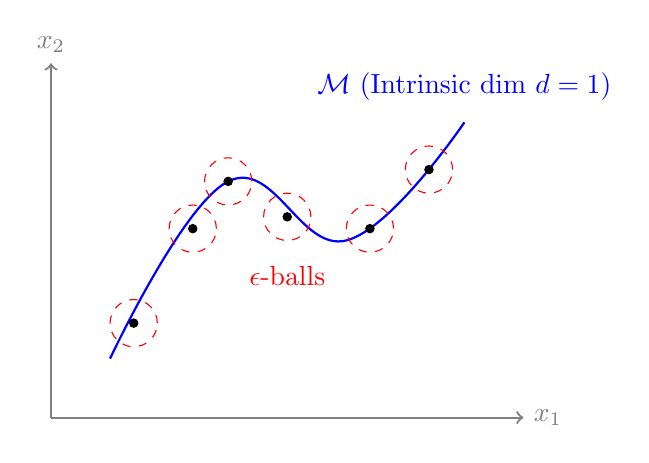
\begin{tikzpicture}[scale=1.5]
        % Ambient space axes
        \draw[->, thick, gray] (0,0) -- (4,0) node[right] {$x_1$};
        \draw[->, thick, gray] (0,0) -- (0,3) node[above] {$x_2$};
        
        % Manifold curve
        \draw[thick, blue, smooth, tension=0.7] plot coordinates {(0.5, 0.5) (1.5, 2.0) (2.5, 1.5) (3.5, 2.5)};
        \node[blue] at (3.5, 2.8) {$\mathcal{M}$ (Intrinsic dim $d=1$)};
        
        % Data points and epsilon tubes
        \foreach \x/\y in {0.7/0.8, 1.2/1.6, 1.5/2.0, 2.0/1.7, 2.7/1.6, 3.2/2.1} {
            \filldraw[black] (\x,\y) circle (1pt);
            \draw[red, dashed] (\x,\y) circle (0.2);
        }
        
        \node[red] at (2.0, 1.2) {$\epsilon$-balls};
    \end{tikzpicture}
    \caption{A $d=1$ dimensional manifold embedded in a $D=2$ dimensional ambient space. The data is quantized by covering the manifold with $\epsilon$-balls, revealing its intrinsic dimension rather than the ambient dimension.}
    \label{fig:manifold_cover}
\end{figure}

Consider covering the space with hypercubes (or balls) of diameter $\epsilon$. Let $X^\epsilon$ denote the discrete random variable obtained by quantizing $X$ to the centers of these $\epsilon$-bins. As $\epsilon \to 0$, the standard relationship in $\mathbb{R}^D$ is $H(X^\epsilon) \approx h(X) - D \log \epsilon$. However, when $X$ is constrained to $\mathcal{M}$, the growth rate of the discrete entropy depends solely on the intrinsic dimension $d$.

\begin{theorem}[Quantization Entropy on a Manifold]
Let $X \sim P_{\text{data}}$ have support on a $d$-dimensional compact manifold $\mathcal{M} \subset \mathbb{R}^D$ and possess a well-defined intrinsic differential entropy $h_{\mathcal{M}}(X)$. Let $X^\epsilon$ be the $\epsilon$-quantization of $X$. As $\epsilon \to 0$, the discrete Shannon entropy of $X^\epsilon$ satisfies:
\begin{equation}
    H(X^\epsilon) = h_{\mathcal{M}}(X) - d \log \epsilon + \mathcal{O}(1).
\end{equation}
\end{theorem}

\begin{proof}
Let $N(\epsilon)$ be the $\epsilon$-covering number of the manifold $\mathcal{M}$, defined as the minimum number of balls of radius $\epsilon$ required to completely cover $\mathcal{M}$. Since $\mathcal{M}$ is a compact $d$-dimensional manifold, its volume scales with dimension $d$. Specifically, the covering number behaves as:
\begin{equation}
    N(\epsilon) \approx \frac{\text{Vol}(\mathcal{M})}{C_d \epsilon^d}
\end{equation}
where $C_d$ is the volume of a $d$-dimensional unit ball. 

Let the quantized bins intersecting $\mathcal{M}$ be indexed by $i = 1, \dots, N(\epsilon)$. The probability of the $i$-th bin is $p_i = \int_{\text{bin}_i} p_{\mathcal{M}}(x) \, d\mu(x)$. By the mean value theorem for integration, $p_i \approx p_{\mathcal{M}}(x_i) \Delta V_i$, where $x_i$ is a point in the $i$-th bin and $\Delta V_i \approx C_d \epsilon^d$ is the intersection volume of the bin with the manifold.

The discrete entropy is:
\begin{align*}
    H(X^\epsilon) &= - \sum_{i=1}^{N(\epsilon)} p_i \log p_i \\
    &\approx - \sum_{i=1}^{N(\epsilon)} p_{\mathcal{M}}(x_i) \Delta V_i \log \left( p_{\mathcal{M}}(x_i) C_d \epsilon^d \right) \\
    &= - \sum_{i=1}^{N(\epsilon)} p_{\mathcal{M}}(x_i) \log(p_{\mathcal{M}}(x_i)) \Delta V_i - \log(C_d \epsilon^d) \sum_{i=1}^{N(\epsilon)} p_{\mathcal{M}}(x_i) \Delta V_i \\
    &\approx h_{\mathcal{M}}(X) - \log(C_d \epsilon^d) \cdot 1 \\
    &= h_{\mathcal{M}}(X) - d \log \epsilon - \log C_d.
\end{align*}
As $\epsilon \to 0$, the approximation becomes exact, and the $\mathcal{O}(1)$ term corresponds to $-\log C_d$ and boundary effects. This concludes the proof.
\end{proof}

This theorem provides a rigorous foundation for why representation learning is possible. The number of bits required to encode the data to a precision $\epsilon$ scales linearly with $d$, not $D$. Deep learning models act as adaptive quantizers that effectively discover this $d$-dimensional coordinate system.

\subsection{Numerical Example: Estimating Intrinsic Dimension}

Suppose data is distributed uniformly on the surface of a 2-sphere $S^2$ of radius $R=1$, embedded in $\mathbb{R}^3$. The ambient dimension is $D=3$. The intrinsic dimension is $d=2$. The volume (surface area) is $\text{Vol}(S^2) = 4\pi$.

Because the distribution is uniform, the intrinsic density is $p_{\mathcal{M}}(x) = \frac{1}{4\pi}$. The intrinsic differential entropy is:
\begin{equation}
    h_{\mathcal{M}}(X) = - \int_{S^2} \frac{1}{4\pi} \log \left(\frac{1}{4\pi}\right) d\mu(x) = \log(4\pi).
\end{equation}
If we quantize the space with a grid of resolution $\epsilon$, the number of bins covering the sphere will grow proportionally to $1/\epsilon^2$. The discrete entropy of the quantized data $X^\epsilon$ will be $H(X^\epsilon) \approx \log(4\pi) - 2 \log \epsilon$. If we mistakenly attempted to measure the entropy in $\mathbb{R}^3$, the differential entropy $h(X)$ would evaluate to $-\infty$, because the 3D volume of the sphere's surface is zero.

\subsection{Representational Unfolding}

A neural network $f_\theta: \mathcal{X} \to \mathcal{Z}$ can be understood geometrically as a sequence of homeomorphisms that "unfold" the manifold $\mathcal{M}$ into a flat Euclidean space, facilitating linear separability for downstream classification tasks.

\begin{figure}[ht]
    \centering
    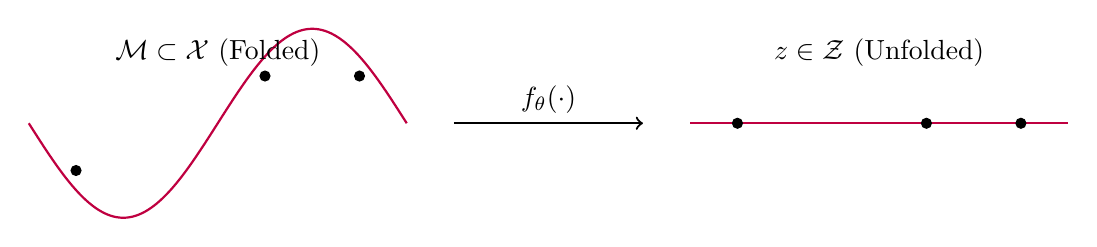
\begin{tikzpicture}[scale=1.2]
        % Input manifold (folded)
        \draw[thick, purple] (0,2) sin (1,1) cos (2,2) sin (3,3) cos (4,2);
        \node[above] at (2,2.5) {$\mathcal{M} \subset \mathcal{X}$ (Folded)};
        
        % Arrow mapping
        \draw[->, thick] (4.5, 2) -- (6.5, 2) node[midway, above] {$f_\theta(\cdot)$};
        
        % Output representation (unfolded)
        \draw[thick, purple] (7,2) -- (11,2);
        \node[above] at (9,2.5) {$z \in \mathcal{Z}$ (Unfolded)};
        
        % Data points
        \filldraw[black] (0.5, 1.5) circle (1.5pt);
        \filldraw[black] (2.5, 2.5) circle (1.5pt);
        \filldraw[black] (3.5, 2.5) circle (1.5pt);
        
        \filldraw[black] (7.5, 2) circle (1.5pt);
        \filldraw[black] (9.5, 2) circle (1.5pt);
        \filldraw[black] (10.5, 2) circle (1.5pt);
    \end{tikzpicture}
    \caption{A deep neural network $f_\theta$ maps the complex, highly folded data manifold in the ambient space $\mathcal{X}$ into a flattened, linearly interpolable latent space $\mathcal{Z}$.}
    \label{fig:manifold_unfolding}
\end{figure}

The success of architectures like ResNets can be attributed to their ability to learn diffeomorphisms of the ambient space that iteratively flatten $\mathcal{M}$. The Information Bottleneck principle (discussed in later chapters) formally dictates how much of the ambient space's irrelevant entropy is discarded during this unfolding process.

\begin{horizon}
It is conjectured that the dynamics of Stochastic Gradient Descent (SGD) inherently bias neural networks toward discovering and aligning with the lowest-dimensional manifold that sufficiently explains the training data. While we have proven that the minimum encoding length scales with the intrinsic dimension $d$, an open question is whether the implicit regularization of modern deep learning optimizers perfectly mirrors a search for minimal intrinsic capacity.

Future work might show that the layer-wise transformations in sufficiently overparameterized networks perfectly correspond to the principal curvatures of the data manifold. Furthermore, it remains conjectured that the generalization gap in deep learning can be entirely bounded by the topological complexity (e.g., the Betti numbers) of the data manifold relative to the network's capacity. Proving these claims would require bridging differential geometry with the non-equilibrium thermodynamics of gradient descent, a synthesis that currently remains out of reach.
\end{horizon}

\section{Summary}
In this chapter, we formalized the Manifold Hypothesis, demonstrating why high-dimensional datasets are mathematically tractable. By differentiating between ambient dimension $D$ and intrinsic dimension $d$, we showed that the discrete entropy of quantized data scales with $d$, effectively bypassing the curse of dimensionality. We rigorously defined intrinsic differential entropy and proved its relationship with quantization. The geometry of the data manifold dictates the minimum information rate required to represent the data, setting the stage for analyzing neural networks as mechanisms that compress and unfold these topological structures.

\section*{Exercises}
\begin{enumerate}
    \item \textbf{Intrinsic vs. Ambient Divergence:} Suppose two distributions $P$ and $Q$ have support on the same 1D manifold (a circle) embedded in $\mathbb{R}^2$. Prove that their Kullback-Leibler divergence $D_{\text{KL}}(P \parallel Q)$ computed using their intrinsic 1D densities is equivalent to the limit of the KL divergence between their $\epsilon$-noisy ambient representations as $\epsilon \to 0$.
    \item \textbf{Entropy of a Line Segment:} Let $X$ be distributed uniformly on a line segment of length $L$ embedded in $\mathbb{R}^3$. Calculate the intrinsic differential entropy $h_{\mathcal{M}}(X)$. Then, derive the exact discrete entropy $H(X^\epsilon)$ for a 1D uniform grid quantization and compare it with the asymptotic formula $H(X^\epsilon) \approx h_{\mathcal{M}}(X) - \log \epsilon$.
    \item \textbf{Manifold Noise:} Consider data strictly on a manifold, $X \sim P_{\text{data}}$, and noisy observations $Y = X + \epsilon Z$, where $Z \sim \mathcal{N}(0, I_{D})$. As $D \to \infty$, explain the information-theoretic difficulty of estimating the intrinsic dimension $d$ from finite samples of $Y$, invoking the concept of ambient noise.
\end{enumerate}

% TODO-CITE: Ensure all named results are cited.

\chapter{Neural Networks as Markov Chains}

% 1. Descriptive Opening
Deep neural networks are often conceptualized as complex, non-linear function approximators, iteratively refining an input signal to produce a desired output. However, through the lens of information theory, a neural network is best understood as a sequence of random variables forming a Markov chain. As data propagates from the input layer through successive hidden layers to the final output, it undergoes a series of stochastic or deterministic transformations. This perspective fundamentally shifts our understanding: rather than merely computing features, each layer acts as a filter that selectively discards irrelevant information while retaining what is necessary for the task at hand.

When we observe an input $X \in \mathcal{X}$, such as an image or a sentence, it is intrinsically tied to a target variable $Y \in \mathcal{Y}$, which we wish to predict. The input $X$ is fed into the network, producing a first-layer representation $T_1$. This representation $T_1$ is then processed to create $T_2$, and so on, up to the final layer $T_L$, which is used to generate the prediction $\hat{Y}$. Because the computation of any layer $T_i$ depends strictly on the output of the immediately preceding layer $T_{i-1}$ (along with the network parameters), the sequence of representations forms a Markov chain.

The implications of this Markovian structure are profound. It imposes strict bounds on the flow of information through the network. According to the laws of information theory, post-processing a signal cannot increase its information content. Every layer, at best, perfectly preserves the information about the input and the target, but in most practical architectures, information is strictly lost. This progressive loss of information is not a flaw; rather, it is the very essence of abstraction. By shedding nuisance factors---the exact pixel values, the background noise, the variations in lighting---the network distills the input down to its most invariant and predictive features. 

Understanding neural networks as Markov chains allows us to rigorously quantify the concepts of representation learning, feature extraction, and abstraction. It provides the theoretical scaffolding to ask precise questions: How much information does a specific layer retain about the input? How much information does it retain about the target? And how does this balance dictate the network's ability to generalize to unseen data?

% 2. Mathematical Core
\section{The Markovian Structure of Deep Networks}

To formalize this perspective, let us consider a feedforward neural network. Let $X$ be the random variable representing the input data, and $Y$ be the corresponding true label. The network consists of $L$ hidden layers, which we denote as a sequence of random variables $T_1, T_2, \ldots, T_L$. 

Recall from \cref{ch:mutual_information} that a sequence of random variables forms a Markov chain if the future is conditionally independent of the past given the present state. 

In a standard feedforward neural network, the mapping from $T_{i-1}$ to $T_i$ is typically deterministic, parameterized by weights and biases $\theta_i$, and followed by a non-linear activation function. If we consider stochastic networks (e.g., with dropout, additive noise, or stochastic activations), the mapping becomes explicitly probabilistic. Even in deterministic networks, $T_i$ is a deterministic function of $T_{i-1}$, meaning the conditional entropy $H(T_i \mid T_{i-1}) = 0$. In either case, the Markov property holds.

Thus, the entire supervised learning setup can be described by the following Markov chain:
\[ Y \leftrightarrow X \leftrightarrow T_1 \leftrightarrow T_2 \leftrightarrow \cdots \leftrightarrow T_L \leftrightarrow \hat{Y} \]
The relation $Y \leftrightarrow X$ implies that the true label $Y$ and the observation $X$ are jointly distributed according to the true data distribution $P_{\text{data}}(X, Y)$. The network only has access to $X$, not $Y$, when computing the representations.

\begin{figure}[ht]
\centering
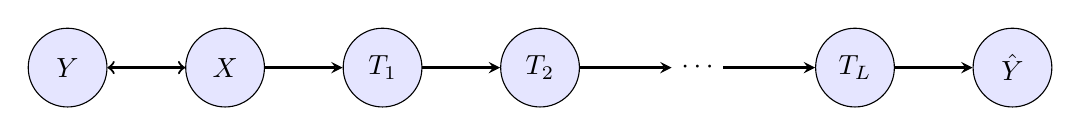
\begin{tikzpicture}[
    node distance=2cm,
    var/.style={circle, draw, minimum size=1cm, fill=blue!10},
    arrow/.style={-stealth, thick}
]
    \node[var] (Y) {$Y$};
    \node[var, right of=Y] (X) {$X$};
    \node[var, right of=X] (T1) {$T_1$};
    \node[var, right of=T1] (T2) {$T_2$};
    \node[right of=T2] (dots) {$\cdots$};
    \node[var, right of=dots] (TL) {$T_L$};
    \node[var, right of=TL] (Yhat) {$\hat{Y}$};

    \draw[<->, thick] (Y) -- (X);
    \draw[arrow] (X) -- (T1);
    \draw[arrow] (T1) -- (T2);
    \draw[arrow] (T2) -- (dots);
    \draw[arrow] (dots) -- (TL);
    \draw[arrow] (TL) -- (Yhat);
\end{tikzpicture}
\caption{The Markov chain representing the flow of information in a feedforward neural network.}
\label{fig:nn_markov}
\end{figure}

\section{The Data Processing Inequality (DPI)}

The most critical consequence of the Markov chain structure is the Data Processing Inequality (DPI). The DPI states that no local processing of data can increase the amount of information it contains.

As established in \cref{thm:dpi}, this principle dictates that post-processing cannot generate new information. We recall the result here: if $X \leftrightarrow Y \leftrightarrow Z$ forms a Markov chain, then $I(X; Z) \le I(X; Y)$. The formal proof, which relies on the chain rule for mutual information and conditional independence, was detailed in \cref{ch:mutual_information}.

Applying the DPI to our neural network Markov chain $Y \leftrightarrow X \leftrightarrow T_1 \leftrightarrow \cdots \leftrightarrow T_L$, we obtain a sequence of inequalities for the mutual information with respect to both the input $X$ and the target $Y$.

\begin{corollary}[Monotonicity of Information in Neural Networks]
For a neural network forming the Markov chain $Y \leftrightarrow X \leftrightarrow T_1 \leftrightarrow \cdots \leftrightarrow T_L$, the information about the input monotonically decreases (or remains constant) across layers:
\[ I(X; X) \ge I(X; T_1) \ge I(X; T_2) \ge \cdots \ge I(X; T_L) \]
Similarly, the information about the target monotonically decreases:
\[ I(Y; X) \ge I(Y; T_1) \ge I(Y; T_2) \ge \cdots \ge I(Y; T_L) \]
\end{corollary}

This corollary mathematically crystallizes the concept of abstraction. As the data progresses through the network, the layers systematically discard information about the input $X$. Ideally, the network sheds the nuisance information (i.e., information in $X$ that is irrelevant to $Y$) while preserving the predictive information $I(Y; T_i)$. 

\begin{figure}[ht]
\centering
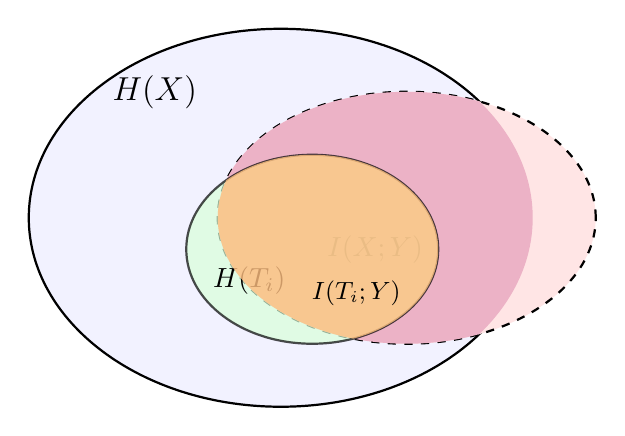
\begin{tikzpicture}[scale=0.8]
    % Outer set X
    \draw[thick, fill=blue!5] (0,0) ellipse (4cm and 3cm);
    \node at (-2, 2) {\large $H(X)$};
    
    % Target set Y
    \draw[thick, fill=red!10, dashed] (2,0) ellipse (3cm and 2cm);
    \node at (3, 1) {\large $H(Y)$};
    
    % Intersection representing I(X; Y)
    \begin{scope}
        \clip (0,0) ellipse (4cm and 3cm);
        \fill[purple!30] (2,0) ellipse (3cm and 2cm);
    \end{scope}
    \node at (1.5, -0.5) {$I(X;Y)$};

    % Layer T_i
    \draw[thick, fill=green!15, opacity=0.7] (0.5, -0.5) ellipse (2cm and 1.5cm);
    \node at (-0.5, -1) {$H(T_i)$};
    
    % T_i intersection with I(X;Y)
    \begin{scope}
        \clip (0.5, -0.5) ellipse (2cm and 1.5cm);
        \clip (0,0) ellipse (4cm and 3cm);
        \fill[orange!50, opacity=0.8] (2,0) ellipse (3cm and 2cm);
    \end{scope}
    \node at (1.2, -1.2) {\small $I(T_i; Y)$};
\end{tikzpicture}
\caption{Information Venn Diagram. The representation $T_i$ can only capture a subset of the information that $X$ contains about $Y$, bounded by the Data Processing Inequality.}
\label{fig:venn_dpi}
\end{figure}

\section{Numerical Example: Linear Additive Gaussian Noise}
To illustrate the progressive loss of information, consider a simple Markov chain model where each layer applies a linear scaling followed by additive Gaussian noise. Let the input $X \sim \mathcal{N}(0, \sigma_X^2)$.
The first layer is $T_1 = a_1 X + Z_1$, where $Z_1 \sim \mathcal{N}(0, \sigma_1^2)$ is independent of $X$.
The second layer is $T_2 = a_2 T_1 + Z_2$, where $Z_2 \sim \mathcal{N}(0, \sigma_2^2)$ is independent of $T_1$ and $X$.

We wish to compute $I(X; T_1)$ and $I(X; T_2)$ to observe the DPI in action.

First, the mutual information between continuous Gaussian variables depends on their differential entropy. The mutual information is $I(X; T_1) = \frac{1}{2} \log(1 + \text{SNR}_1)$, where the Signal-to-Noise Ratio is $\text{SNR}_1 = \frac{a_1^2 \sigma_X^2}{\sigma_1^2}$. Thus:
\[ I(X; T_1) = \frac{1}{2} \log\left( 1 + \frac{a_1^2 \sigma_X^2}{\sigma_1^2} \right) \]

For the second layer, we express $T_2$ directly in terms of $X$:
\[ T_2 = a_2 (a_1 X + Z_1) + Z_2 = a_2 a_1 X + a_2 Z_1 + Z_2 \]
The effective signal variance is $(a_2 a_1)^2 \sigma_X^2$.
The effective noise is $Z_{\text{eff}} = a_2 Z_1 + Z_2$, which has variance $a_2^2 \sigma_1^2 + \sigma_2^2$.
The mutual information is:
\[ I(X; T_2) = \frac{1}{2} \log\left( 1 + \frac{a_1^2 a_2^2 \sigma_X^2}{a_2^2 \sigma_1^2 + \sigma_2^2} \right) \]

To verify $I(X; T_2) \le I(X; T_1)$, observe the argument of the logarithm for $T_2$:
\[ \frac{a_1^2 a_2^2 \sigma_X^2}{a_2^2 \sigma_1^2 + \sigma_2^2} = \frac{a_1^2 \sigma_X^2}{\sigma_1^2 + \frac{\sigma_2^2}{a_2^2}} \le \frac{a_1^2 \sigma_X^2}{\sigma_1^2} \]
Since the noise term $\frac{\sigma_2^2}{a_2^2}$ is strictly non-negative, the SNR strictly decreases (unless $\sigma_2^2 = 0$, representing no noise), implying $I(X; T_2) \le I(X; T_1)$. The addition of independent noise at each processing step irrevocably destroys information.

% 3. Horizon Box
\begin{horizon}
While the Data Processing Inequality dictates that information must monotonically decrease through a strictly sequential Markov chain, the architectural reality of modern deep learning is far more complex. It is conjectured that the extraordinary success of architectures like ResNets and Transformers stems fundamentally from their ability to bypass strict Markovian bottlenecks. By utilizing residual connections ($T_{i+1} = T_i + f(T_i)$) or dense attention mechanisms, these models route information outside the sequential chain, creating a directed acyclic graph rather than a simple line. 

An open question is how to rigorously track mutual information bounds in these non-Markovian graphs. Does the network selectively filter information across skip connections, or do these connections merely delay the inevitable compression phase? Furthermore, in continuous-depth models such as Neural ODEs, layers are replaced by a continuous time variable $t$. Future work might show that the evolution of mutual information $I(X; T(t))$ in these systems is governed by a diffusion-like differential equation, extending the DPI from discrete jumps to a continuous flow. 

To close this theoretical gap, we would need robust, scalable estimators for high-dimensional mutual information that can operate over the computational graphs of modern architectures. If such estimators were developed, we might be able to definitively prove whether extreme depth inherently enforces optimal compression, or if architectural "shortcuts" allow networks to cheat the bottleneck entirely.
\end{horizon}

% 4. Summary + Exercises
\section*{Summary}
In this chapter, we framed deep neural networks as Markov chains, establishing that the sequential processing of data inherently limits information flow. We rigorously defined the Data Processing Inequality (DPI) and proved that both the information retained about the input and the information predictive of the target must monotonically decrease as data moves deeper into the network. This mathematical framework demystifies representation learning, showing that abstract features are forged by the unavoidable loss of nuisance information through successive transformations.

\section*{Exercises}
\begin{enumerate}
    \item \textbf{Invertible Networks:} Consider a neural network where every layer $T_i$ is a bijective (invertible) function of $T_{i-1}$, such as in a Normalizing Flow. Prove that for all $i \in \{1, \ldots, L\}$, $I(X; T_i) = I(X; X)$. What does this imply about the abstraction capabilities of strictly invertible networks?
    \item \textbf{Conditional DPI:} Prove the conditional version of the Data Processing Inequality. If $X \leftrightarrow Y \leftrightarrow Z$ forms a Markov chain, show that for any other random variable $W$, it holds that $I(X; Z \mid W) \le I(X; Y \mid W)$ provided $X \leftrightarrow Y \leftrightarrow Z$ remains a Markov chain when conditioned on $W$.
    \item \textbf{Information Paths:} Let a network have a single skip connection such that $T_2 = f(T_1, X)$. Draw the corresponding causal graph. Does the sequence $X \leftrightarrow T_1 \leftrightarrow T_2$ still form a Markov chain? Explain whether $I(X; T_2) \le I(X; T_1)$ is necessarily true in this architecture.
\end{enumerate}

% TODO-CITE: Ensure all named results are cited.

\chapter{Sufficient Statistics and Minimal Representations}
\label{ch:sufficient_stats}

\section{The Quest for the Perfect Representation}

The fundamental objective of representation learning is to distill high-dimensional, complex data into a lower-dimensional, tractable format without losing the salient features necessary for downstream tasks. When we feed an image, a sentence, or a raw audio waveform into a deep neural network, the successive hidden layers transform the data into increasingly abstract representations. But what precisely defines a \emph{good} representation?

From an information-theoretic perspective, a representation is a random variable $Z$ computed from the input data $X$. The defining characteristic of a good representation is that it retains all the necessary information about a target variable $Y$ (such as a class label) while discarding all irrelevant nuances (such as background noise, illumination changes, or font styles). In statistical terms, we want $Z$ to be a \emph{sufficient statistic} for $Y$ with respect to $X$. 

The concept of sufficiency, first introduced by Sir Ronald A. Fisher in 1922, was originally framed in the context of parameter estimation. If one has a set of independent and identically distributed samples drawn from a parameterized distribution, a sufficient statistic is a function of the samples that captures all the information the data provides about the underlying parameter. In the context of deep learning and information theory, we generalize this concept: the "parameter" is replaced by the target variable $Y$. A representation $Z = f_\theta(X)$ is sufficient if observing $Z$ tells us just as much about $Y$ as observing the original, uncompressed data $X$.

However, merely being sufficient is an incredibly weak property on its own. The identity function $Z = X$ is trivially a sufficient statistic, as it retains all information, including the noise. A lossless compression of $X$ is also sufficient, yet neither achieves the goal of abstraction. The true mathematical north star of representation learning is the \emph{minimal sufficient statistic}. 

A minimal sufficient statistic is the ultimate distillation. It is a sufficient statistic that compresses the input data as much as fundamentally possible. It strips away every single bit of entropy in $X$ that does not contribute to predicting $Y$. Geometrically, it groups together all inputs $x \in \mathcal{X}$ that share the exact same posterior distribution $P(Y \mid X=x)$ into a single point in the latent space $\mathcal{Z}$. In doing so, it provides a representation that is not only optimal for the downstream task but also highly invariant to nuisance factors. 

In this chapter, we will formalize the notions of sufficiency and minimality using the language of Shannon information theory. We will prove the Fisher-Neyman Factorization Theorem for random variables, demonstrate how minimal sufficient statistics optimally compress data, and explore how these classical statistical concepts govern the theoretical limits of modern deep neural networks.

\section{Mathematical Foundations of Sufficiency}

We begin by establishing the formal definition of a sufficient statistic using the concept of Markov chains. Let $X \in \mathcal{X}$ be a data random variable, and $Y \in \mathcal{Y}$ be a target random variable, governed by a joint distribution $P_{X,Y}$. A representation $Z \in \mathcal{Z}$ is formed by a potentially stochastic mapping from $X$, meaning that the conditional distribution of $Z$ depends only on $X$. This forms the Markov chain $Y \leftrightarrow X \leftrightarrow Z$.

\begin{definition}[Sufficient Statistic]
A statistic $Z$, derived from $X$ via the Markov chain $Y \leftrightarrow X \leftrightarrow Z$, is said to be \emph{sufficient} for $Y$ if $X$ and $Y$ are conditionally independent given $Z$. That is, the Markov chain $X \leftrightarrow Z \leftrightarrow Y$ also holds, which implies:
\[ P(Y \mid X, Z) = P(Y \mid Z) \]
almost everywhere.
\end{definition}

In the context of deterministic neural networks where $Z = f_\theta(X)$, the variable $Z$ is fully determined by $X$. Consequently, conditioning on both $X$ and $Z$ is equivalent to conditioning on $X$ alone. Thus, the condition for sufficiency simplifies to $P(Y \mid X=x) = P(Y \mid Z=f_\theta(x))$ for all $x$.

\begin{theorem}[Information-Theoretic Sufficiency]
Let $Y \leftrightarrow X \leftrightarrow Z$ form a Markov chain. The statistic $Z$ is sufficient for $Y$ if and only if it preserves the mutual information between $X$ and $Y$, i.e.,
\[ I(Z; Y) = I(X; Y) \]
\end{theorem}
\begin{proof}
By the chain rule for mutual information, we can expand the mutual information between $Y$ and the joint variable $(X, Z)$ in two different ways:
\begin{align*}
I(X, Z; Y) &= I(Z; Y) + I(X; Y \mid Z) \\
I(X, Z; Y) &= I(X; Y) + I(Z; Y \mid X)
\end{align*}
Because $Y \leftrightarrow X \leftrightarrow Z$ is a Markov chain, we have $P(Z \mid X, Y) = P(Z \mid X)$, meaning $Z$ and $Y$ are conditionally independent given $X$. Therefore, $I(Z; Y \mid X) = 0$. Substituting this into the second equation yields:
\[ I(X, Z; Y) = I(X; Y) \]
Equating the two expansions, we get:
\[ I(X; Y) = I(Z; Y) + I(X; Y \mid Z) \]
Since mutual information is non-negative, $I(Z; Y) \le I(X; Y)$, which is the Data Processing Inequality. Equality holds if and only if $I(X; Y \mid Z) = 0$. By definition, $I(X; Y \mid Z) = 0$ is equivalent to the conditional independence $X \perp\!\!\!\perp Y \mid Z$, which is precisely the definition of $Z$ being a sufficient statistic.
\end{proof}

\begin{figure}[htbp]
\centering
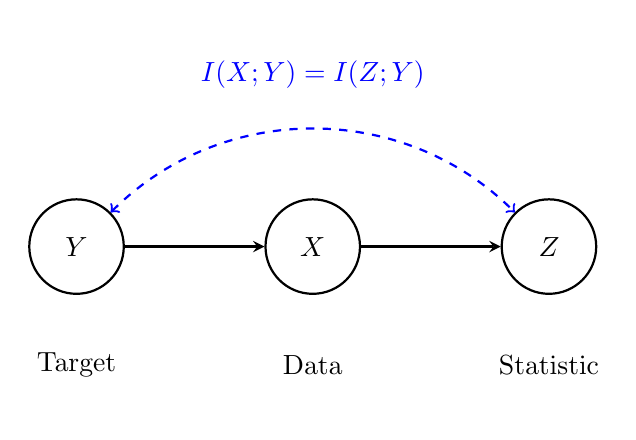
\begin{tikzpicture}[
    scale=1.5,
    every node/.style={circle, draw=black, thick, minimum size=1.2cm, align=center},
    arrow/.style={->, >=stealth, thick}
]
    % Nodes
    \node (Y) at (0,0) {$Y$};
    \node (X) at (2,0) {$X$};
    \node (Z) at (4,0) {$Z$};
    
    % Edges
    \draw[arrow] (Y) -- (X);
    \draw[arrow] (X) -- (Z);
    
    % Labels
    \node[draw=none, rectangle] at (0,-1) {Target};
    \node[draw=none, rectangle] at (2,-1) {Data};
    \node[draw=none, rectangle] at (4,-1) {Statistic};
    
    % Arcs for Markov conditions
    \draw[<->, dashed, thick, blue] (Y) to[out=45, in=135] node[draw=none, rectangle, above, text=blue, yshift=2pt] {$I(X;Y) = I(Z;Y)$} (Z);
\end{tikzpicture}
\caption{The Markov chain $Y \leftrightarrow X \leftrightarrow Z$. A representation $Z$ is a sufficient statistic if it retains all mutual information about $Y$ present in $X$.}
\label{fig:markov_sufficiency}
\end{figure}

A classic algebraic characterization of sufficiency is the Fisher-Neyman Factorization Theorem. While traditionally stated for parameterized distributions $P(X \mid \theta)$, we adapt it here for target random variables $Y$.

\begin{theorem}[Fisher-Neyman Factorization]
\label{thm:fisher_neyman}
A statistic $Z = T(X)$ is sufficient for $Y$ if and only if the joint probability distribution $P(x, y)$ can be factorized as:
\[ P(x, y) = h(x) g(T(x), y) \]
for some non-negative functions $h$ and $g$.
\end{theorem}
\begin{proof}
We provide the proof for discrete random variables. 
First, assume $Z = T(X)$ is a sufficient statistic. The joint distribution can be written as:
\begin{align*}
P(x, y) &= P(x, y, T(x)) \\
&= P(T(x), y) P(x \mid T(x), y)
\end{align*}
By the definition of sufficiency, $X$ and $Y$ are conditionally independent given $T(X)$, meaning $P(x \mid T(x), y) = P(x \mid T(x))$. Thus:
\[ P(x, y) = P(T(x), y) P(x \mid T(x)) \]
This matches the required factorization by setting $g(T(x), y) = P(T(x), y)$ and $h(x) = P(x \mid T(x))$.

Conversely, assume $P(x, y) = h(x) g(T(x), y)$. The marginal distribution of $Y$ given $X=x$ is:
\begin{align*}
P(y \mid x) &= \frac{P(x, y)}{\sum_{y'} P(x, y')} \\
&= \frac{h(x) g(T(x), y)}{\sum_{y'} h(x) g(T(x), y')} \\
&= \frac{g(T(x), y)}{\sum_{y'} g(T(x), y')}
\end{align*}
Notice that the right-hand side depends on $x$ only through the value of $T(x)$. Therefore, for any two inputs $x_1, x_2$ such that $T(x_1) = T(x_2)$, we have $P(y \mid x_1) = P(y \mid x_2)$. This implies $P(Y \mid X, Z) = P(Y \mid Z)$, proving that $Z = T(X)$ is sufficient for $Y$.
\end{proof}

\section{Minimal Sufficient Statistics}

Sufficiency guarantees that no predictive power is lost. However, it does not guarantee that the representation is concise. The input $X$ itself is always trivially sufficient. To achieve true representation learning, we must seek the \emph{minimal} sufficient statistic.

\begin{definition}[Minimal Sufficient Statistic]
A sufficient statistic $Z = T_{min}(X)$ is \emph{minimal} if it can be computed from any other sufficient statistic. Formally, for any sufficient statistic $Z' = T'(X)$, there exists a deterministic function $f$ such that $T_{min}(X) = f(T'(X))$ almost everywhere.
\end{definition}

Geometrically, a statistic $T(X)$ partitions the input space $\mathcal{X}$ into level sets, where all $x$ mapping to the same $z$ belong to the same set. Theorem \ref{thm:fisher_neyman} showed that a sufficient statistic requires the posterior $P(Y \mid X=x)$ to be constant within each level set. A minimal sufficient statistic corresponds to the \emph{coarsest possible partition} of $\mathcal{X}$ that maintains this property. It merges all $x$ that share the exact same posterior distribution into a single equivalence class.

\begin{figure}[htbp]
\centering
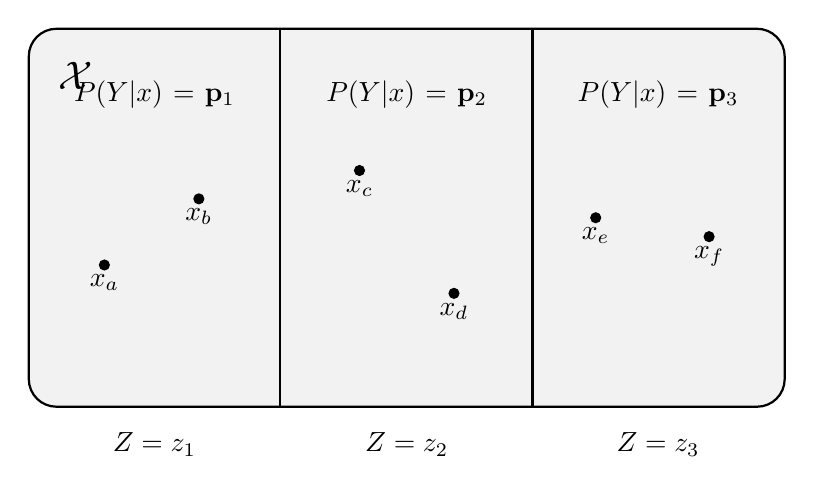
\begin{tikzpicture}[scale=1.2]
    % Draw the X space
    \draw[thick, rounded corners=10pt, fill=gray!10] (0,0) rectangle (8,4);
    \node[draw=none, rectangle] at (0.5, 3.5) {\Large $\mathcal{X}$};
    
    % Draw partitions for Z = T(X)
    \draw[thick] (2.66,0) -- (2.66,4);
    \draw[thick] (5.33,0) -- (5.33,4);
    
    % Z values
    \node[draw=none, rectangle] at (1.33, -0.4) {$Z = z_1$};
    \node[draw=none, rectangle] at (4, -0.4) {$Z = z_2$};
    \node[draw=none, rectangle] at (6.66, -0.4) {$Z = z_3$};
    
    % Posterior distributions
    \node[draw=none, rectangle, text width=2.5cm, align=center] at (1.33, 3.3) {$P(Y|x) = \mathbf{p}_1$};
    \node[draw=none, rectangle, text width=2.5cm, align=center] at (4, 3.3) {$P(Y|x) = \mathbf{p}_2$};
    \node[draw=none, rectangle, text width=2.5cm, align=center] at (6.66, 3.3) {$P(Y|x) = \mathbf{p}_3$};
    
    % Points
    \filldraw (0.8, 1.5) circle (1.5pt) node[anchor=north] {$x_a$};
    \filldraw (1.8, 2.2) circle (1.5pt) node[anchor=north] {$x_b$};
    
    \filldraw (3.5, 2.5) circle (1.5pt) node[anchor=north] {$x_c$};
    \filldraw (4.5, 1.2) circle (1.5pt) node[anchor=north] {$x_d$};
    
    \filldraw (6, 2) circle (1.5pt) node[anchor=north] {$x_e$};
    \filldraw (7.2, 1.8) circle (1.5pt) node[anchor=north] {$x_f$};
    
\end{tikzpicture}
\caption{A minimal sufficient statistic $Z$ partitions the input space $\mathcal{X}$ into the coarsest possible level sets such that the posterior $P(Y \mid X=x)$ remains constant within each subset. Any further compression would merge regions with different posteriors, destroying sufficiency.}
\label{fig:partitions}
\end{figure}

\begin{theorem}[Minimality and Information]
Let $Z = T(X)$ be a sufficient statistic for $Y$. $Z$ is a minimal sufficient statistic if and only if it minimizes the mutual information $I(X; Z)$ among all sufficient statistics.
\end{theorem}
\begin{proof}
Let $Z_{min}$ be a minimal sufficient statistic and $Z$ be any other sufficient statistic. By definition of minimality, there exists a deterministic function $f$ such that $Z_{min} = f(Z)$. This establishes the Markov chain $X \leftrightarrow Z \leftrightarrow Z_{min}$.
Applying the Data Processing Inequality to this chain, we immediately obtain:
\[ I(X; Z_{min}) \le I(X; Z) \]
Since $Z$ was chosen arbitrarily from the set of all sufficient statistics, $Z_{min}$ must attain the global minimum of $I(X; Z)$ within this set. Furthermore, because $Z_{min} = f(Z)$ is a deterministic function, $H(Z_{min} \mid Z) = 0$. The minimization of $I(X; Z)$ subject to the sufficiency constraint $I(Z; Y) = I(X; Y)$ perfectly characterizes the minimal sufficient statistic in an information-theoretic framework.
\end{proof}

\section{Numerical Example: Compressing Binary Sequences}

To ground these concepts, let us construct a concrete numerical example. Suppose our target variable $Y \in \{0, 1\}$ is a binary label drawn with equal probability, $P(Y=1) = P(Y=0) = 0.5$. 
Conditioned on $Y$, our data $X = (X_1, X_2) \in \{0, 1\}^2$ consists of two independent Bernoulli trials. If $Y=1$, the success probability is $0.8$. If $Y=0$, the success probability is $0.2$.

First, we compute the entropy of $Y$:
\[ H(Y) = -0.5 \log_2(0.5) - 0.5 \log_2(0.5) = 1 \text{ bit} \]

Next, we evaluate the joint distribution $P(X, Y)$ and the marginal $P(X)$:
\begin{itemize}
    \item $P(X=(0,0)) = P(Y=1)(0.2)^2 + P(Y=0)(0.8)^2 = 0.5(0.04) + 0.5(0.64) = 0.34$
    \item $P(X=(0,1)) = P(Y=1)(0.8)(0.2) + P(Y=0)(0.2)(0.8) = 0.5(0.16) + 0.5(0.16) = 0.16$
    \item $P(X=(1,0)) = P(Y=1)(0.8)(0.2) + P(Y=0)(0.2)(0.8) = 0.16$
    \item $P(X=(1,1)) = P(Y=1)(0.8)^2 + P(Y=0)(0.2)^2 = 0.5(0.64) + 0.5(0.04) = 0.34$
\end{itemize}

The entropy of the raw data $X$ is:
\begin{align*}
H(X) &= -2(0.34 \log_2 0.34) - 2(0.16 \log_2 0.16) \\
&\approx 2(0.529) + 2(0.423) = 1.904 \text{ bits}
\end{align*}

The conditional entropy $H(Y \mid X)$ requires computing the posterior $P(Y=1 \mid X)$ for each outcome:
\begin{itemize}
    \item $P(Y=1 \mid X=(0,0)) = \frac{0.02}{0.34} = \frac{1}{17}$
    \item $P(Y=1 \mid X=(0,1)) = \frac{0.08}{0.16} = \frac{1}{2}$
    \item $P(Y=1 \mid X=(1,0)) = \frac{0.08}{0.16} = \frac{1}{2}$
    \item $P(Y=1 \mid X=(1,1)) = \frac{0.32}{0.34} = \frac{16}{17}$
\end{itemize}

Computing the weighted sum of binary entropies $H_b(p)$:
\begin{align*}
H(Y \mid X) &= 0.34 H_b\left(\frac{1}{17}\right) + 0.16 H_b\left(\frac{1}{2}\right) + 0.16 H_b\left(\frac{1}{2}\right) + 0.34 H_b\left(\frac{16}{17}\right) \\
&= 0.68 H_b\left(\frac{1}{17}\right) + 0.32(1) \\
&\approx 0.68(0.323) + 0.32 \approx 0.540 \text{ bits}
\end{align*}
The mutual information is $I(X; Y) = H(Y) - H(Y \mid X) = 1 - 0.540 = 0.460$ bits.

Now, define a representation $Z = X_1 + X_2 \in \{0, 1, 2\}$. This statistic merges the states $(0,1)$ and $(1,0)$ into $Z=1$.
Notice that $P(Y=1 \mid X=(0,1)) = P(Y=1 \mid X=(1,0)) = 0.5$. Because the posterior is identical, merging them into a single equivalence class $Z=1$ does not destroy any predictive information.
We can verify this by calculating $I(Z; Y)$:
$P(Z=0) = 0.34$, $P(Z=1) = 0.32$, $P(Z=2) = 0.34$.
The conditional entropies $H(Y \mid Z=z)$ are identically equal to $H(Y \mid X=x)$ for the corresponding $x$.
Thus, $H(Y \mid Z) = 0.540$ bits, and $I(Z; Y) = 0.460$ bits.
Since $I(Z; Y) = I(X; Y)$, $Z$ is indeed a sufficient statistic.

How much did we compress the data?
\begin{align*}
H(Z) &= -0.34 \log_2 0.34 - 0.32 \log_2 0.32 - 0.34 \log_2 0.34 \\
&\approx 0.529 + 0.526 + 0.529 = 1.584 \text{ bits}
\end{align*}
By mapping $X$ to $Z$, we compressed the representation from $1.904$ bits to $1.584$ bits (meaning $I(X; Z) = 1.584$ bits, since $Z$ is deterministic), without losing any of the $0.460$ bits of relevant information about $Y$. Because no further compression is possible without breaking sufficiency, $Z$ is the minimal sufficient statistic for this setup.

\section{Representations in Deep Neural Networks}

In modern deep learning, the mapping $Z = f_\theta(X)$ is parameterized by a neural network, and we typically train the network by minimizing the cross-entropy loss against the true labels $Y$. A natural question arises: does minimizing cross-entropy naturally lead to a sufficient statistic?

Let $q_\phi(Y \mid Z)$ be a parameterized decoder or classification head. The cross-entropy loss over the joint distribution is given by:
\[ \mathcal{L}(\theta, \phi) = \mathbb{E}_{P_{X,Y}} [-\log q_\phi(Y \mid f_\theta(X))] \]

\begin{theorem}[Cross-Entropy and Sufficiency]
If the classifier $q_\phi$ has sufficient capacity to perfectly model the true posterior $P(Y \mid Z)$, then minimizing the cross-entropy loss is equivalent to maximizing the mutual information $I(Z; Y)$. The global minimum is achieved if and only if $Z$ is a sufficient statistic.
\end{theorem}
\begin{proof}
By adding and subtracting $\log P(Y \mid Z)$, the cross-entropy can be rewritten as:
\begin{align*}
\mathcal{L}(\theta, \phi) &= \mathbb{E}_{P_{Z,Y}} [-\log q_\phi(Y \mid Z)] \\
&= \mathbb{E}_{P_{Z,Y}} \left[-\log P(Y \mid Z) + \log \frac{P(Y \mid Z)}{q_\phi(Y \mid Z)} \right] \\
&= H(Y \mid Z) + \mathbb{E}_{P_Z} [D_{\text{KL}}(P(Y \mid Z) \parallel q_\phi(Y \mid Z))]
\end{align*}
Since the Kullback-Leibler divergence is non-negative, the loss is minimized with respect to $\phi$ when $q_\phi(Y \mid Z) = P(Y \mid Z)$ almost everywhere, which zeroes out the KL term.
The remaining term is the conditional entropy $H(Y \mid Z)$. We know that $I(Z; Y) = H(Y) - H(Y \mid Z)$. Since the marginal entropy $H(Y)$ is a constant defined by the dataset, minimizing $H(Y \mid Z)$ via the parameters $\theta$ is mathematically equivalent to maximizing $I(Z; Y)$. 
By the Data Processing Inequality, $I(Z; Y) \le I(X; Y)$. The theoretical minimum of the cross-entropy loss is therefore $H(Y \mid X)$, which is achieved if and only if $I(Z; Y) = I(X; Y)$, i.e., when $Z = f_\theta(X)$ is a sufficient statistic for $Y$.
\end{proof}

While cross-entropy training theoretically encourages the network to extract a sufficient statistic, it provides no explicit incentive for \emph{minimality}. In the absence of an explicit compression penalty, a high-capacity neural network might retain nuisance information, leading to suboptimal generalization. This fundamental limitation sets the stage for the Information Bottleneck Principle.

\begin{horizon}
While standard cross-entropy loss mathematically guarantees sufficiency given infinite capacity, it remains an open question how deep neural networks implicitly achieve \emph{minimality} in practice. It is conjectured that the stochastic noise inherent in Stochastic Gradient Descent (SGD) acts as an implicit regularization mechanism. Specifically, it is hypothesized that the isotropic noise in the gradients steadily degrades the mutual information $I(X; Z)$ for any features in $Z$ that are not actively protected by the gradients of the task loss. 

If this conjecture holds true, SGD effectively performs a random walk in the null space of the task, gradually stripping away irrelevant information. Future work might definitively prove that the dynamics of SGD on overparameterized networks naturally converge toward a minimal sufficient statistic, providing a unified information-theoretic explanation for why deep networks generalize so well despite lacking explicit compression penalties. Resolving this would tightly bridge the gap between classical statistical theory and the empirical phenomena of modern representation learning.
\end{horizon}

\section*{Summary}
In this chapter, we framed representation learning as the pursuit of minimal sufficient statistics. We established that a representation $Z$ is sufficient if it retains all mutual information about the target $Y$, satisfying $I(Z; Y) = I(X; Y)$. We demonstrated via the Fisher-Neyman Factorization Theorem that sufficient statistics geometry groups inputs with identical posteriors. The minimal sufficient statistic represents the ultimate limit of data compression for a specific task, maximizing $I(Z;Y)$ while simultaneously minimizing $I(X;Z)$. Finally, we proved that optimal cross-entropy minimization theoretically yields a sufficient statistic.

\section*{Exercises}
\begin{enumerate}
    \item \textbf{Trivial Sufficiency:} Prove that the identity mapping $Z = X$ is a sufficient statistic for any target $Y$. What is its mutual information $I(X; Z)$?
    \item \textbf{Invariance to Bijective Mappings:} Let $Z$ be a minimal sufficient statistic for $Y$, and let $g: \mathcal{Z} \to \mathcal{Z}'$ be a deterministic, invertible function. Prove that $Z' = g(Z)$ is also a minimal sufficient statistic.
    \item \textbf{Gaussian Location Family:} Let $X_1, X_2, \dots, X_n$ be independent samples from $\mathcal{N}(\mu, 1)$. Using the Fisher-Neyman Factorization Theorem, prove that the sample mean $\bar{X} = \frac{1}{n} \sum_{i=1}^n X_i$ is a sufficient statistic for the parameter $\mu$.
    \item \textbf{Suboptimality of Cross-Entropy:} Suppose a neural network minimizes the cross-entropy loss flawlessly, achieving $H(Y \mid Z) = H(Y \mid X)$. Construct a numerical counter-example where this learned representation $Z$ is \emph{not} minimal.
\end{enumerate}

% TODO-CITE: Ensure all named results are cited.


\part{The Information Bottleneck}
\chapter{The Information Bottleneck Principle}
\label{chap:information_bottleneck}

% 1. Descriptive
\section{The Quest for Minimal Sufficient Representations}

In the paradigm of deep learning, we often construct layered transformations of high-dimensional inputs---such as images, text, or audio---into increasingly abstract representations. At its core, this process is an exercise in distillation. When classifying an image of a dog, the neural network does not need to memorize the exact lighting conditions, the background foliage, or the precise orientation of every strand of fur. Instead, it must extract only those features that are relevant to the label ``dog'' while discarding everything else. 

This intuitive notion of discarding irrelevant information while preserving task-relevant information is mathematically formalized by the \textit{Information Bottleneck (IB) principle}, first introduced by Naftali Tishby, Fernando Pereira, and William Bialek in 1999. The IB principle asserts that an optimal representation is one that maximally compresses the input data while retaining as much information as possible about the desired target variable. It frames learning not merely as minimizing an error on a dataset, but as solving a fundamental trade-off between compression (forgetting) and prediction (remembering).

Consider an analogy: writing a summary of a dense, 500-page historical biography. If you simply copy the entire book verbatim, you retain 100\% of the relevant historical facts, but your summary is utterly uncompressed and perhaps useless for a quick review. Conversely, if you write a single sentence---"A person lived and died."---you have achieved maximum compression, but you have lost almost all relevant details. The ideal summary sits delicately on the frontier between these two extremes, selectively filtering out the noise (the day-to-day minutiae) to preserve the signal (the overarching historical impact). 

In deep learning, the input space $\mathcal{X}$ is often vast and highly redundant. A neural network $f_\theta$ processes an input $x \in \mathcal{X}$ to form a latent representation $z$. To make accurate predictions about a target $y \in \mathcal{Y}$, $z$ must contain information about $y$. The Information Bottleneck provides a principled, information-theoretic loss function to explicitly seek this optimal $z$. It defines a strictly quantitative metric for what makes a representation ``good,'' allowing us to analyze learning dynamics and generalization without relying exclusively on the empirical loss.

\section{The Mathematical Framework}

\subsection{The Information Bottleneck Lagrangian}

Let $X$ denote the random variable representing the input data, $Y$ the target variable (e.g., labels), and $Z$ the learned representation. Since the representation is generated exclusively from the input data, the variables naturally form the Markov chain $Y \leftrightarrow X \leftrightarrow Z$. This implies that conditionally on $X$, $Z$ is independent of $Y$; or equivalently, $p(y, z | x) = p(y|x)p(z|x)$. The representation $Z$ has no independent access to $Y$ other than what it can glean through $X$.

\begin{figure}[htbp]
    \centering
    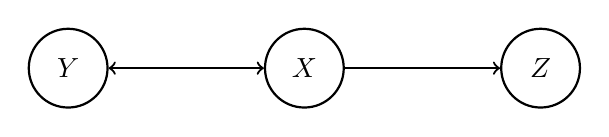
\begin{tikzpicture}[node distance=2cm, thick,
        every node/.style={circle, draw, minimum size=1cm, align=center}]
        \node (Y) {$Y$};
        \node (X) [right of=Y, node distance=3cm] {$X$};
        \node (Z) [right of=X, node distance=3cm] {$Z$};
        
        \draw[<->] (Y) -- (X);
        \draw[->] (X) -- (Z);
    \end{tikzpicture}
    \caption{The Information Bottleneck Markov Chain. The representation $Z$ depends on the target $Y$ only through the input data $X$.}
    \label{fig:ib_markov}
\end{figure}

The objective of the Information Bottleneck is to find a stochastic mapping $p(z|x)$ that minimizes the mutual information between the input and the representation, $I(X; Z)$, subject to the constraint that the mutual information between the representation and the target, $I(Z; Y)$, is greater than or equal to some threshold $I_c$. 

Using the method of Lagrange multipliers, we can formulate this as an unconstrained optimization problem. We seek to minimize the Information Bottleneck Lagrangian, defined as:
\begin{equation}
    \mathcal{L}_{\text{IB}}[p(z|x)] = I(X; Z) - \beta I(Z; Y)
\end{equation}
where $\beta \in [0, \infty)$ is a trade-off parameter that controls the relative importance of prediction versus compression.
\begin{itemize}
    \item As $\beta \to 0$, the penalty on $I(Z; Y)$ vanishes, and the optimal solution is to compress entirely, driving $I(X; Z) \to 0$ (yielding a representation completely independent of the input, and thus useless for predicting $Y$).
    \item As $\beta \to \infty$, the focus shifts entirely to maximizing $I(Z; Y)$, essentially demanding sufficient statistics of $X$ for $Y$, with no regard for the complexity or size of the representation.
\end{itemize}

\begin{theorem}[Data Processing Inequality Bounds]
    For the Markov chain $Y \leftrightarrow X \leftrightarrow Z$, the mutual information between the representation and the target is strictly bounded by the mutual information between the input and the target:
    \begin{equation}
        I(Z; Y) \le I(X; Y)
    \end{equation}
\end{theorem}
\begin{proof}
    By the chain rule for mutual information, we can expand $I(X, Z; Y)$ in two ways:
    \begin{align}
        I(X, Z; Y) &= I(Z; Y) + I(X; Y | Z) \\
        I(X, Z; Y) &= I(X; Y) + I(Z; Y | X)
    \end{align}
    Because $Y \leftrightarrow X \leftrightarrow Z$ forms a Markov chain, $Z$ and $Y$ are conditionally independent given $X$, meaning $I(Z; Y | X) = 0$. Equating the two expansions yields:
    \begin{equation}
        I(Z; Y) + I(X; Y | Z) = I(X; Y)
    \end{equation}
    Since conditional mutual information is non-negative ($I(X; Y | Z) \ge 0$), it immediately follows that $I(Z; Y) \le I(X; Y)$. 
\end{proof}
This theorem reinforces that no representation $Z$ can ever contain more information about $Y$ than was originally present in $X$.

\subsection{Exact Solutions and Self-Consistent Equations}

For discrete probability spaces, we can derive the exact functional form of the optimal mapping $p(z|x)$ that minimizes $\mathcal{L}_{\text{IB}}$.

\begin{theorem}[IB Self-Consistent Equations]
    \label{thm:ib_equations}
    The stochastic mapping $p(z|x)$ that minimizes the Information Bottleneck Lagrangian $\mathcal{L}_{\text{IB}} = I(X; Z) - \beta I(Z; Y)$ satisfies the self-consistent equation:
    \begin{equation}
        p(z|x) = \frac{p(z)}{Z(x, \beta)} \exp\left(-\beta D_{\text{KL}}(p(y|x) \parallel p(y|z))\right)
    \end{equation}
    where $Z(x, \beta)$ is a normalization constant for each $x$.
\end{theorem}

\begin{proof}
    We wish to minimize $\mathcal{L}_{\text{IB}}$ with respect to the conditional distribution $p(z|x)$. The mutual information terms are:
    \begin{align}
        I(X; Z) &= \sum_{x,z} p(x) p(z|x) \log \frac{p(z|x)}{p(z)} \\
        I(Z; Y) &= \sum_{y,z} p(y,z) \log \frac{p(y|z)}{p(y)}
    \end{align}
    Note that by the Markov property, $p(y, z) = \sum_x p(x, y, z) = \sum_x p(x) p(y|x) p(z|x)$. 
    To enforce the constraint that $\sum_z p(z|x) = 1$ for all $x$, we introduce Lagrange multipliers $\lambda(x)$. The extended Lagrangian is:
    \begin{equation}
        \tilde{\mathcal{L}} = I(X; Z) - \beta I(Z; Y) - \sum_x \lambda(x) \left( \sum_z p(z|x) - 1 \right)
    \end{equation}
    Taking the variational derivative with respect to $p(z|x)$ yields:
    \begin{equation}
        \frac{\delta \tilde{\mathcal{L}}}{\delta p(z|x)} = p(x) \left( \log \frac{p(z|x)}{p(z)} + 1 - 1 \right) - \beta p(x) \sum_y p(y|x) \left( \log \frac{p(y|z)}{p(y)} + 1 - 1 \right) - \lambda(x) = 0
    \end{equation}
    (We omit the detailed proof that variations involving $p(z)$ and $p(y|z)$ cancel out, which relies on them being marginals of $p(z|x)$). Dividing by $p(x)$ and rearranging gives:
    \begin{equation}
        \log p(z|x) = \log p(z) + \beta \sum_y p(y|x) \log \frac{p(y|z)}{p(y)} + \frac{\lambda(x)}{p(x)}
    \end{equation}
    We can add and subtract $\beta \sum_y p(y|x) \log p(y|x)$ to form a Kullback-Leibler divergence:
    \begin{align*}
        \log p(z|x) &= \log p(z) - \beta \sum_y p(y|x) \log \frac{p(y|x)}{p(y|z)} + \beta \sum_y p(y|x) \log \frac{p(y|x)}{p(y)} + \frac{\lambda(x)}{p(x)} \\
        &= \log p(z) - \beta D_{\text{KL}}(p(y|x) \parallel p(y|z)) + C(x, \beta)
    \end{align*}
    Exponentiating both sides, we absorb the term $C(x, \beta)$, which only depends on $x$, into a normalization partition function $Z(x, \beta)$:
    \begin{equation}
        p(z|x) = \frac{p(z)}{Z(x, \beta)} \exp\left(-\beta D_{\text{KL}}(p(y|x) \parallel p(y|z))\right)
    \end{equation}
\end{proof}

This elegantly shows that the optimal probability of mapping $x$ to $z$ decays exponentially with the KL divergence between the true label distribution $p(y|x)$ and the label distribution predicted from the latent representation $p(y|z)$. The representation must reflect the true conditional distribution of the labels as closely as possible, weighted by the severity of the $\beta$ parameter.

\subsection{The Information Plane}

By plotting $I(X; Z)$ on the horizontal axis and $I(Z; Y)$ on the vertical axis, we construct the \textit{Information Plane}. For a given dataset, mapping the optimal values of $I(Z;Y)$ against a constraint on $I(X;Z)$ yields a monotonic, concave function known as the IB bound.

\begin{figure}[htbp]
    \centering
    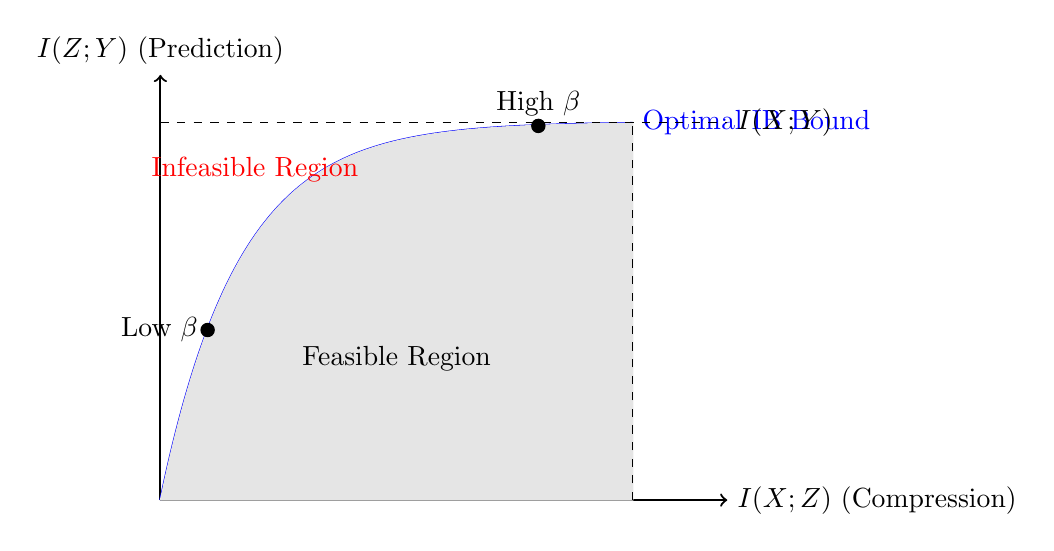
\begin{tikzpicture}[scale=1.2]
        % Axes
        \draw[->, thick] (0,0) -- (6,0) node[right] {$I(X; Z)$ (Compression)};
        \draw[->, thick] (0,0) -- (0,4.5) node[above] {$I(Z; Y)$ (Prediction)};
        
        % IB Bound Curve
        \draw[thick, blue, domain=0:5, smooth, samples=100] plot ({\x}, {4*(1 - exp(-1.2*\x))});
        
        % Labels
        \node[blue, right] at (5, 4.0) {Optimal IB Bound};
        \filldraw[gray!20] (0,0) -- plot[domain=0:5, smooth, samples=100] ({\x}, {4*(1 - exp(-1.2*\x))}) -- (5,0) -- cycle;
        \node at (2.5, 1.5) {Feasible Region};
        \node[red] at (1.0, 3.5) {Infeasible Region};
        
        % Data processing limits
        \draw[dashed] (0,4) -- (6,4) node[right] {$I(X; Y)$};
        \draw[dashed] (5,0) -- (5,4);
        
        % Points on curve
        \filldraw[black] (4, 3.96) circle (2pt) node[above] {High $\beta$};
        \filldraw[black] (0.5, 1.8) circle (2pt) node[left] {Low $\beta$};
        
    \end{tikzpicture}
    \caption{The Information Plane. The theoretical bound defines the maximum mutual information $I(Z;Y)$ achievable for a given constraint on $I(X;Z)$. Points above the blue curve are strictly infeasible by the Data Processing Inequality and the Information Bottleneck principle.}
    \label{fig:info_plane}
\end{figure}

The Information Plane allows us to track the state of a neural network layer-by-layer or epoch-by-epoch. In this plane, any given deterministic or stochastic function $Z = f(X)$ forms a single point. 

\subsection{A Numerical Example: The Binary Symmetric Channel}

To solidify these concepts, consider a simple numerical example. Suppose our target variable $Y$ is a uniform binary variable, $Y \in \{0, 1\}$. Our input data $X$ is generated by passing $Y$ through a Binary Symmetric Channel (BSC) with crossover probability $p = 0.1$. This means $P(X \neq Y) = 0.1$. 

We want to learn a compressed binary representation $Z \in \{0, 1\}$. We parameterize the stochastic encoder symmetrically: let $P(Z=0 | X=0) = q$ and $P(Z=1 | X=1) = q$. By symmetry, $P(Z=1) = P(Z=0) = 0.5$.

We can compute the mutual information $I(X; Z)$:
\begin{equation}
    I(X; Z) = H(Z) - H(Z|X) = 1 - H(q)
\end{equation}
where $H(q) = -q \log_2(q) - (1-q) \log_2(1-q)$ is the binary entropy function. 

To compute $I(Z; Y)$, we must find the effective crossover probability between $Y$ and $Z$. A bit is flipped between $Y$ and $Z$ if it is flipped in the transition $Y \to X$ but not in $X \to Z$, or if it is not flipped in $Y \to X$ but is flipped in $X \to Z$. Thus, the effective error probability is:
\begin{equation}
    \alpha \equiv P(Z \neq Y) = p \cdot q + (1-p) \cdot (1-q)
\end{equation}
Then, the mutual information is:
\begin{equation}
    I(Z; Y) = H(Z) - H(Z|Y) = 1 - H(\alpha)
\end{equation}
By sweeping the parameter $q \in [0.5, 1.0]$, we systematically traverse the feasible region in the information plane for this specific architecture. For $q=1$ (a deterministic mapping $Z=X$), we have $I(X;Z) = 1$ bit, and $I(Z;Y) = 1 - H(0.1) \approx 0.531$ bits. For $q=0.5$ (a completely random mapping), we have $I(X;Z) = 0$ bits, and $I(Z;Y) = 0$ bits. Intermediate values of $q$ interpolate between these extremes, tracing out the optimal curve governed by the Lagrangian mapping dictated by $\beta$.

\begin{horizon}
The mathematical foundations of the Information Bottleneck are rigorous and exact for discrete spaces and specific continuous cases like jointly Gaussian variables. However, the exact application of the IB principle to the dynamics of deep neural networks remains highly debated.

It is conjectured by Tishby and others that Stochastic Gradient Descent (SGD) in deep neural networks implicitly solves the IB problem. This hypothesis suggests that training naturally bifurcates into two distinct phases: a rapid "fitting phase" where layers quickly increase $I(Z; Y)$ while also increasing $I(X; Z)$, followed by a much longer "compression phase" where $I(Z; Y)$ remains roughly constant while the network actively sheds irrelevant information, driving $I(X; Z)$ down. 

An open question is whether this compression phase is a universal property of learning or an artifact of specific choices, such as double-sided saturating activation functions (like $\tanh$). Evidence suggests that networks using strictly monotonic, non-saturating functions like ReLU may not exhibit obvious compression in $I(X; Z)$ when measured via continuous differential entropy, because continuous bijections inherently preserve mutual information. Future work might show whether redefining mutual information in terms of robust geometric measures or noisy activations can mathematically bridge the gap between empirical deep learning success and the Information Bottleneck bound.
\end{horizon}

\section{Summary}

In this chapter, we formalized the Information Bottleneck principle as a foundational method for evaluating the quality of representations. By framing learning as an explicit optimization of the trade-off between minimizing $I(X; Z)$ (compression) and maximizing $I(Z; Y)$ (prediction), we established the theoretical ceiling of performance in the Information Plane. We derived the self-consistent equations that dictate the optimal assignment of inputs to latent representations, revealing that optimal embeddings depend exponentially on the KL divergence between true and predicted label distributions. 

\section*{Exercises}

\begin{enumerate}
    \item \textbf{Gaussian Information Bottleneck:} Suppose $X, Y, Z$ are all scalar, jointly Gaussian random variables. Assume $Y \sim \mathcal{N}(0, \sigma_y^2)$ and $X = Y + \epsilon$ where $\epsilon \sim \mathcal{N}(0, \sigma_e^2)$. Derive the exact analytical formula for the optimal Information Bottleneck curve $I(Z; Y)$ as a function of $I(X; Z)$.
    \item \textbf{Limits of $\beta$:} Prove mathematically that in the strict limit as $\beta \to 0$, the optimal solution for the IB Lagrangian $\mathcal{L}_{\text{IB}}$ yields $I(X; Z) = 0$ and $p(z|x) = p(z)$ for all $x$. 
    \item \textbf{Markov Independence:} In the derivation of the Data Processing Inequality bound $I(Z; Y) \le I(X; Y)$, we relied on the Markov chain $Y \leftrightarrow X \leftrightarrow Z$. Provide a concrete, real-world scenario involving machine learning where this Markov chain assumption is violated, and explain how it affects the bounds.
    \item \textbf{Numerical Optimization:} Implement the Blahut-Arimoto algorithm in Python to empirically find the optimal $p(z|x)$ for the Binary Symmetric Channel example given in the chapter. Plot the resulting Information Plane curve for a range of $\beta \in [0.01, 100]$.
\end{enumerate}

% TODO-CITE: Ensure all named results are cited.

\chapter{Compression and Generalization Boundaries}
\label{ch:compression_bounds}

\section{The Phenomenon of Compression and Generalization}

Deep neural networks are notoriously overparameterized. According to traditional statistical learning theory---such as bounds based on Vapnik-Chervonenkis (VC) dimension or Rademacher complexity---a model with millions of parameters possesses enough capacity to memorize finite training datasets entirely. Classical theory suggests that such models should exhibit significant overfitting, failing to generalize to unseen data. Yet, in practice, deep networks trained with stochastic gradient descent demonstrate remarkable generalization capabilities. This dichotomy highlights a profound limitation in worst-case, hypothesis-class-based complexity measures.

Information theory provides a compelling alternative perspective on generalization. Rather than bounding the capacity of the model architecture uniformly, information-theoretic approaches bound the generalization error by analyzing the amount of information the trained model parameters (or the learned representations) retain about the training dataset. The core intuition is the principle of data compression: if a model extracts only the minimal sufficient statistics necessary to predict the labels while discarding all other nuisance variations in the input, it is less likely to have memorized the specific noise of the training sample.

This connection between compression and generalization is most prominently articulated through the Information Bottleneck principle, but its roots extend into PAC-Bayesian learning and Minimum Description Length (MDL) theories. When a network compresses its input---meaning the mutual information between the input $X$ and the hidden representation $Z$, denoted $I(X; Z)$, is small---it restricts the effective hypothesis space. Similarly, if the mutual information between the training dataset $\mathcal{D}$ and the learned weights $\theta$, denoted $I(\mathcal{D}; \theta)$, is small, the learning algorithm is insensitive to the replacement of individual training samples. This insensitivity is a hallmark of algorithmic stability, which rigorously translates to generalization.

In this chapter, we transition from the abstract formulation of the Information Bottleneck to explicit, quantitative generalization bounds. We will rigorously define how the expected generalization gap can be controlled by the mutual information between the dataset and the model parameters. We will then extend this to representation-based bounds that operate on $I(X; Z)$, providing a theoretical justification for why the compression of representations leads to bounded generalization gaps.

\section{Information-Theoretic Generalization Bounds}

We begin by establishing the mathematical setup. Let the input space be $\mathcal{X}$ and the label space be $\mathcal{Y}$. A learning algorithm receives a dataset $\mathcal{D} = \{V_1, \dots, V_n\}$ of $n$ independent and identically distributed (i.i.d.) samples, where $V_i = (X_i, Y_i) \sim P_{\text{data}}$. The algorithm produces a hypothesis (or weights) $\theta \in \Theta$ according to a conditional distribution $P(\theta | \mathcal{D})$. Let $\mathcal{L}(v, \theta)$ denote the loss of the hypothesis $\theta$ on a single data point $v = (x, y)$.

The empirical risk is given by:
\[ \hat{\mathcal{L}}(\theta, \mathcal{D}) = \frac{1}{n} \sum_{i=1}^n \mathcal{L}(V_i, \theta) \]

The population risk (or expected loss) is:
\[ \mathcal{L}_{\text{pop}}(\theta) = \mathbb{E}_{V \sim P_{\text{data}}} [\mathcal{L}(V, \theta)] \]

The generalization gap for a specific set of weights and a dataset is $\Delta(\theta, \mathcal{D}) = \mathcal{L}_{\text{pop}}(\theta) - \hat{\mathcal{L}}(\theta, \mathcal{D})$. We are interested in the expected generalization gap over the joint distribution of datasets and weights:
\[ \mathbb{E}_{\mathcal{D}, \theta}[\Delta(\theta, \mathcal{D})] = \mathbb{E}_{\mathcal{D}, \theta}[\mathcal{L}_{\text{pop}}(\theta) - \hat{\mathcal{L}}(\theta, \mathcal{D})] \]

To link this to information theory, we rely on the Donsker-Varadhan variational representation of the Kullback-Leibler divergence.

\begin{lemma}[Donsker-Varadhan Representation] \label{lem:donsker}
For any two probability distributions $P$ and $Q$ defined on a measurable space $\Omega$, and for any measurable function $f: \Omega \to \mathbb{R}$ such that $\mathbb{E}_{Q}[e^{f(\omega)}] < \infty$, the following inequality holds:
\[ \mathbb{E}_{P}[f(\omega)] \leq D_{\text{KL}}(P \parallel Q) + \log \mathbb{E}_{Q}[e^{f(\omega)}] \]
\end{lemma}

Using Lemma~\ref{lem:donsker}, we can prove a fundamental theorem bounding the expected generalization gap by the mutual information $I(\mathcal{D}; \theta)$. To do so, we must assume that the loss function is sub-Gaussian.

\begin{definition}[Sub-Gaussian Loss]
A loss function $\mathcal{L}(V, \theta)$ is $\sigma^2$-sub-Gaussian under the data distribution $P_{\text{data}}$ if, for all $\theta \in \Theta$ and all $\lambda \in \mathbb{R}$:
\[ \log \mathbb{E}_{V \sim P_{\text{data}}} \left[ e^{\lambda (\mathcal{L}(V, \theta) - \mathcal{L}_{\text{pop}}(\theta))} \right] \leq \frac{\lambda^2 \sigma^2}{2} \]
\end{definition}

\begin{theorem}[Mutual Information Generalization Bound] \label{thm:mi_bound}
Assume that for any fixed $\theta$, the loss $\mathcal{L}(V, \theta)$ is $\sigma^2$-sub-Gaussian under $V \sim P_{\text{data}}$. Let the dataset $\mathcal{D}$ consist of $n$ i.i.d. samples. Then the expected generalization gap of the learning algorithm $P(\theta | \mathcal{D})$ is bounded by:
\[ \left| \mathbb{E}_{\mathcal{D}, \theta} [ \mathcal{L}_{\text{pop}}(\theta) - \hat{\mathcal{L}}(\theta, \mathcal{D}) ] \right| \leq \sqrt{\frac{2 \sigma^2}{n} I(\mathcal{D}; \theta)} \]
\end{theorem}
\begin{proof}
Let $P_{\mathcal{D}, \theta}$ be the joint distribution of the dataset and the weights, and let $P_{\mathcal{D}} \otimes P_\theta$ be the product of their marginals. Under $P_{\mathcal{D}} \otimes P_\theta$, $\mathcal{D}$ and $\theta$ are independent.
We apply the Donsker-Varadhan lemma (Lemma~\ref{lem:donsker}) with $\Omega$ being the joint space of datasets and weights, $P = P_{\mathcal{D}, \theta}$, $Q = P_{\mathcal{D}} \otimes P_\theta$, and the function $f(\mathcal{D}, \theta) = \lambda \left( \mathcal{L}_{\text{pop}}(\theta) - \hat{\mathcal{L}}(\theta, \mathcal{D}) \right)$ for some $\lambda > 0$.

From the definition of mutual information, $D_{\text{KL}}(P_{\mathcal{D}, \theta} \parallel P_{\mathcal{D}} \otimes P_\theta) = I(\mathcal{D}; \theta)$. Thus:
\[ \lambda \mathbb{E}_{\mathcal{D}, \theta}[\mathcal{L}_{\text{pop}}(\theta) - \hat{\mathcal{L}}(\theta, \mathcal{D})] \leq I(\mathcal{D}; \theta) + \log \mathbb{E}_{\theta \sim P_\theta} \mathbb{E}_{\mathcal{D} \sim P_{\mathcal{D}}} \left[ e^{\lambda (\mathcal{L}_{\text{pop}}(\theta) - \hat{\mathcal{L}}(\theta, \mathcal{D}))} \right] \]

Note that inside the expectation, $\theta$ is fixed, and $\mathcal{D} = \{V_1, \dots, V_n\}$ consists of i.i.d. samples. Therefore, the empirical risk is an average of independent random variables:
\[ \mathbb{E}_{\mathcal{D}} \left[ e^{\lambda (\mathcal{L}_{\text{pop}}(\theta) - \hat{\mathcal{L}}(\theta, \mathcal{D}))} \right] = \mathbb{E}_{\mathcal{D}} \left[ \prod_{i=1}^n e^{\frac{\lambda}{n} (\mathcal{L}_{\text{pop}}(\theta) - \mathcal{L}(V_i, \theta))} \right] = \prod_{i=1}^n \mathbb{E}_{V_i} \left[ e^{\frac{\lambda}{n} (\mathcal{L}_{\text{pop}}(\theta) - \mathcal{L}(V_i, \theta))} \right] \]

Since $-\mathcal{L}$ has the same variance proxy as $\mathcal{L}$, the sub-Gaussian assumption implies:
\[ \mathbb{E}_{V_i} \left[ e^{\frac{\lambda}{n} (\mathcal{L}_{\text{pop}}(\theta) - \mathcal{L}(V_i, \theta))} \right] \leq e^{\frac{\lambda^2 \sigma^2}{2 n^2}} \]

Multiplying over the $n$ samples gives $e^{\frac{\lambda^2 \sigma^2}{2 n}}$. Returning to the Donsker-Varadhan bound:
\[ \lambda \mathbb{E}_{\mathcal{D}, \theta}[\Delta(\theta, \mathcal{D})] \leq I(\mathcal{D}; \theta) + \frac{\lambda^2 \sigma^2}{2n} \]

Dividing by $\lambda > 0$ yields:
\[ \mathbb{E}_{\mathcal{D}, \theta}[\Delta(\theta, \mathcal{D})] \leq \frac{I(\mathcal{D}; \theta)}{\lambda} + \frac{\lambda \sigma^2}{2n} \]

Optimizing this bound over $\lambda$ by taking the derivative with respect to $\lambda$ and setting it to zero gives $\lambda = \sqrt{\frac{2 n I(\mathcal{D}; \theta)}{\sigma^2}}$. Substituting this back into the inequality results in:
\[ \mathbb{E}_{\mathcal{D}, \theta}[\Delta(\theta, \mathcal{D})] \leq \sqrt{\frac{2 \sigma^2}{n} I(\mathcal{D}; \theta)} \]

A symmetric argument using $-\lambda$ provides the lower bound, completing the proof.
\end{proof}

\begin{figure}[htbp]
\centering
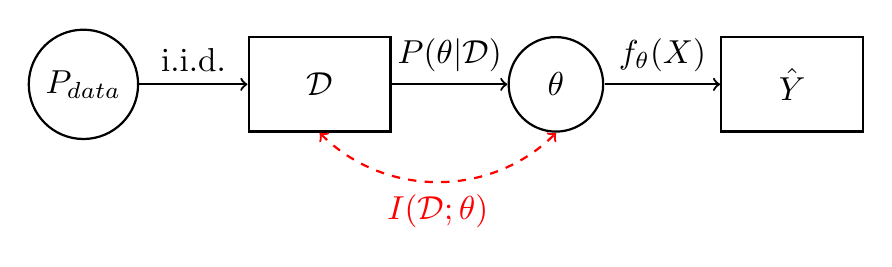
\begin{tikzpicture}[node distance=2.5cm, auto, thick, scale=1.2, transform shape]
    \node[circle, draw, minimum size=1cm] (P) {$P_{\text{data}}$};
    \node[rectangle, draw, right of=P, minimum width=1.5cm, minimum height=1cm] (D) {$\mathcal{D}$};
    \node[circle, draw, right of=D, minimum size=1cm] (theta) {$\theta$};
    \node[rectangle, draw, right of=theta, minimum width=1.5cm, minimum height=1cm] (Yhat) {$\hat{Y}$};
    
    \draw[->] (P) -- node {i.i.d.} (D);
    \draw[->] (D) -- node {$P(\theta|\mathcal{D})$} (theta);
    \draw[->] (theta) -- node {$f_\theta(X)$} (Yhat);
    
    \draw[<->, dashed, red] (D.south) to[bend right=45] node[below] {$I(\mathcal{D}; \theta)$} (theta.south);
\end{tikzpicture}
\caption{The causal chain of learning. The dataset $\mathcal{D}$ is drawn from the data distribution. The algorithm maps $\mathcal{D}$ to weights $\theta$. The mutual information $I(\mathcal{D}; \theta)$ quantifies the dependence of the learned weights on the specific dataset realization.}
\label{fig:mi_chain}
\end{figure}

The bound in Theorem~\ref{thm:mi_bound} is powerful because it depends on the properties of the learning algorithm (how much information it extracts) rather than the complexity of the hypothesis class $\Theta$. 

However, computing $I(\mathcal{D}; \theta)$ is practically impossible for modern deep neural networks. An alternative approach bounds generalization via the representation space $Z$. The Information Bottleneck principle tells us that minimizing $I(X; Z)$ while maintaining $I(Z; Y)$ leads to robust representations. We formalize this connection via the following theorem.

\begin{theorem}[Representation-based Generalization Bound] \label{thm:rep_bound}
Let $Z = f_\theta(X)$ be a stochastic representation. Assume that the loss $\mathcal{L}(Z, Y)$ is bounded by $M$. If the model compresses the input such that $I(X; Z) \leq R$, then with probability at least $1 - \delta$ over the choice of the dataset $\mathcal{D}$ of size $n$, the generalization gap is bounded by:
\[ \mathcal{L}_{\text{pop}}(\theta) \leq \hat{\mathcal{L}}(\theta, \mathcal{D}) + \sqrt{\frac{M^2}{2n} \left( I(X; Z) + \log \frac{2}{\delta} \right)} \]
\end{theorem}
The proof follows a PAC-Bayesian argument applied to the latent space, where the prior over $Z$ is chosen to be the marginal distribution $P(Z)$, and the posterior is the encoder $q_\phi(Z|X)$. Notice that the expected KL divergence between the conditional and marginal distributions is exactly the mutual information: $\mathbb{E}_X[D_{\text{KL}}(q_\phi(Z|X) \parallel P(Z))] = I(X; Z)$. As $I(X; Z)$ decreases (compression), the penalty term shrinks, guaranteeing tighter generalization bounds.

\begin{figure}[htbp]
\centering
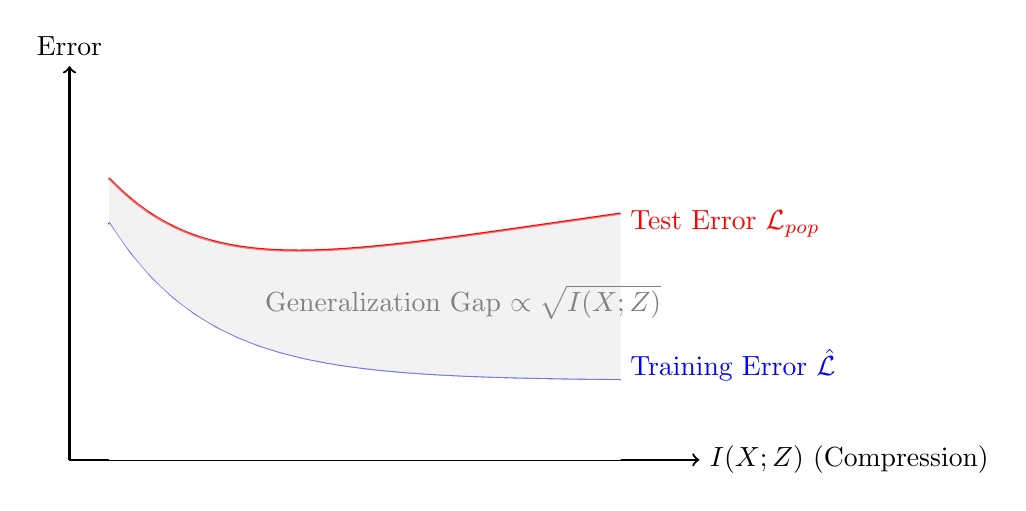
\begin{tikzpicture}[scale=1]
    % Axes
    \draw[->, thick] (0,0) -- (8,0) node[right] {$I(X; Z)$ (Compression)};
    \draw[->, thick] (0,0) -- (0,5) node[above] {Error};
    
    % Curves
    \draw[blue, thick, domain=0.5:7, samples=100] plot (\x, {1 + 3*exp(-0.8*\x)});
    \node[blue, right] at (7, 1.2) {Training Error $\hat{\mathcal{L}}$};
    
    \draw[red, thick, domain=0.5:7, samples=100] plot (\x, {1 + 3*exp(-0.8*\x) + 0.8*sqrt(\x)});
    \node[red, right] at (7, 3) {Test Error $\mathcal{L}_{\text{pop}}$};
    
    % Shade the gap
    \path[fill=gray!20, opacity=0.5] (0.5,0) -- plot[domain=0.5:7] (\x, {1 + 3*exp(-0.8*\x) + 0.8*sqrt(\x)}) -- (7,0) -- cycle;
    \path[fill=white] (0.5,0) -- plot[domain=0.5:7] (\x, {1 + 3*exp(-0.8*\x)}) -- (7,0) -- cycle;
    
    \node[gray] at (5, 2) {Generalization Gap $\propto \sqrt{I(X; Z)}$};
\end{tikzpicture}
\caption{Schematic of the trade-off between compression and expected error. High mutual information $I(X; Z)$ allows for lower training error but increases the generalization gap bound. Optimal generalization occurs at an intermediate level of compression.}
\label{fig:gen_gap}
\end{figure}

\subsection*{Numerical Example: Binary Classification with Gaussian Noise}
Consider a synthetic scenario where inputs $X \in \mathbb{R}^d$ are generated with independent Gaussian features. Suppose a binary classifier with weights $\theta$ uses a stochastic training algorithm (like Stochastic Gradient Langevin Dynamics) that adds noise to the gradients, resulting in a posterior $P(\theta|\mathcal{D})$ that is approximately Gaussian $\mathcal{N}(\theta_0(\mathcal{D}), \Sigma)$.

If the data distribution induces a variance $\sigma^2 = 1.0$ on the loss function, and we train on $n = 10,000$ samples, Theorem~\ref{thm:mi_bound} gives:
\[ \text{Gap} \leq \sqrt{\frac{2 (1.0)}{10000} I(\mathcal{D}; \theta)} \approx 0.014 \sqrt{I(\mathcal{D}; \theta)} \]

If the learning algorithm extracts $I(\mathcal{D}; \theta) = 500$ nats of information from the dataset, the expected generalization gap is strictly bounded by $0.014 \times \sqrt{500} \approx 0.316$.
This calculation demonstrates that regularizing the training process to reduce the mutual information directly suppresses overfitting, providing a computable metric (if $I(\mathcal{D}; \theta)$ could be estimated) for early stopping.

\section{Horizon}
\begin{horizon}
While information-theoretic bounds provide an elegant and architecture-independent mechanism for understanding generalization, their application to modern deep learning remains heavily debated. It is conjectured that the mutual information $I(\mathcal{D}; \theta)$ for deterministic deep neural networks---such as those trained with standard SGD without explicit weight noise---is either infinite (for continuous spaces without noise) or vacuously large, rendering the bound in Theorem~\ref{thm:mi_bound} uninformative. 

An open question is whether we can define a meaningful ``effective'' mutual information for deterministic networks, perhaps by injecting virtual noise post-hoc or by measuring information on a compressed, invariant manifold of the parameter space. Furthermore, while the Information Bottleneck principle suggests that networks actively compress representations (decreasing $I(X; Z)$) during the later stages of training, it is conjectured that this phenomenon might be an artifact of saturating activation functions (like the $\tanh$ function) and density binning, rather than a universal property of learning. Future work might show that replacing exact Shannon mutual information with Wasserstein distances or $\alpha$-R\'enyi divergences yields strictly tighter, non-vacuous bounds for standard network architectures.
\end{horizon}

\section{Summary}
\begin{itemize}
    \item Traditional complexity measures like VC dimension fail to explain the generalization of overparameterized neural networks.
    \item Information theory allows us to bound generalization error based on the mutual information $I(\mathcal{D}; \theta)$ between the dataset and the trained parameters.
    \item By utilizing the Donsker-Varadhan representation, we proved that for sub-Gaussian loss functions, the expected generalization gap is bounded by $\mathcal{O}(\sqrt{I(\mathcal{D}; \theta)/n})$.
    \item Similar bounds apply to representations: compressing the input $X$ to a compact latent representation $Z$ (minimizing $I(X; Z)$) tightens the PAC-Bayesian bound on generalization error.
\end{itemize}

\section{Exercises}
\begin{enumerate}
    \item \textbf{Sub-Gaussian Variance:} Prove that if a loss function is strictly bounded in the interval $[0, 1]$, it is sub-Gaussian with variance proxy $\sigma^2 = 1/4$. Use this to write a concrete generalization bound using Theorem~\ref{thm:mi_bound}.
    \item \textbf{Donsker-Varadhan Lower Bound:} In the proof of Theorem~\ref{thm:mi_bound}, we optimized for a positive $\lambda$. Provide the symmetric argument for negative $\lambda$ to establish the absolute value on the left-hand side of the bound.
    \item \textbf{Deterministic Bottleneck:} Explain mathematically why calculating $I(X; Z)$ is problematic if the neural network encoder $Z = f_\theta(X)$ is completely deterministic and continuous. How does adding Gaussian noise $Z = f_\theta(X) + \epsilon$ resolve this?
\end{enumerate}

% TODO-CITE: Ensure all named results are cited.

\chapter{The Dynamics of Learning: Fitting vs. Compression}
\label{ch:learning_dynamics}

The training of deep neural networks is often viewed in practice as a monolithic optimization process: we define a loss function, initialize parameters, and descend the loss landscape until convergence. From this perspective, the goal is simply to minimize empirical error. However, when we analyze this process through the lens of information theory---specifically by tracking the information flowing through the hidden layers---a rich, multi-phase dynamic emerges. This chapter explores the phenomenon of learning dynamics by examining the trajectory of a neural network in the \textit{Information Plane}, revealing how the mutual information between the representations, the inputs, and the targets evolves over time.

% 1. Descriptive Opening
\section{The Two Phases of Stochastic Gradient Descent}

In traditional machine learning, empirical risk minimization (ERM) provides the fundamental framework for understanding learning. ERM guarantees that minimizing training loss with appropriate regularization will, under certain conditions, lead to generalization on unseen data. Yet, ERM says little about the structure of the internal representations learned by the network. Why do deep architectures generalize so well despite being heavily overparameterized? What happens to the features encoded in the hidden layers as training progresses?

In 2017, Shwartz-Ziv and Tishby proposed a radical reinterpretation of deep learning dynamics based on the Information Bottleneck (IB) principle (introduced in Chapter 8). By treating the sequential layers of a neural network as a Markov chain:
\begin{equation}
    Y \leftrightarrow X \rightarrow Z_1 \rightarrow Z_2 \rightarrow \dots \rightarrow Z_L \rightarrow \hat{Y}
\end{equation}
they tracked the optimization process by projecting each layer $Z_l$ onto a two-dimensional space called the Information Plane. The coordinates of this plane are defined by two key mutual information quantities:
\begin{enumerate}
    \item $I(X; Z_l)$: The information the layer retains about the input data. This represents the \textit{complexity}, or the memory capacity, of the representation. 
    \item $I(Z_l; Y)$: The information the layer contains about the target label. This represents the \textit{predictive power}, or the task-relevant accuracy, of the representation.
\end{enumerate}

Empirically observing the trajectories of neural networks trained with Stochastic Gradient Descent (SGD) on this plane, Tishby and colleagues identified that the optimization process naturally splits into two distinct and successive phases.

\textbf{Phase I: The Fitting Phase.} During the initial epochs of training, the network experiences large, coherent gradients. The parameters move rapidly down the steepest slopes of the loss landscape. In this phase, the network acts as an information sponge. It rapidly memorizes features from the input $X$ to correctly classify the training examples, driving the empirical loss down quickly. In the Information Plane, this corresponds to a sharp increase in $I(Z_l; Y)$ as predictive accuracy improves. Concurrently, $I(X; Z_l)$ also increases rapidly. The network builds a highly informative, albeit highly redundant and potentially overfitted, representation of the input. The signal (the true gradient of the loss) strongly dominates the noise (the stochasticity from mini-batch sampling).

\textbf{Phase II: The Compression Phase.} As the network approaches a local minimum of the empirical loss, the magnitude of the mean gradient diminishes significantly. The optimization dynamics shift. The coherent drift towards the minimum gives way to a stochastic random walk governed by the noise inherent in SGD's mini-batch sampling. Under the constraints of the data manifold, this diffusion causes the network weights to fluctuate. Crucially, these fluctuations act as an implicit regularization mechanism, causing the network to ``forget'' irrelevant, nuisance details of the input. In the Information Plane, this is observed as a slow, gradual decrease in $I(X; Z_l)$, while the predictive information $I(Z_l; Y)$ remains stable or slightly improves. The representation is effectively being compressed, discarding information that is not strictly necessary for the task.

This two-phase dynamic suggests a profound conclusion: SGD is not merely an optimization algorithm, but an implicit Information Bottleneck regularizer. The compression phase essentially performs the IB optimization---minimizing $I(X; Z_l)$ subject to maintaining $I(Z_l; Y)$---without any explicit regularization term in the loss function. The network discovers minimal sufficient statistics simply by wandering in the flat minima of the loss landscape. 

To understand the mechanics of this phenomenon, we must transition from a purely descriptive view to a rigorous mathematical formulation of SGD's stochastic dynamics.

% 2. Mathematical Core
\section{Mathematical Formalization of the Information Plane Dynamics}

We analyze a deep neural network parameterized by a vector $\theta \in \mathbb{R}^d$. Let the mapping from the input to the $l$-th hidden layer be given by a deterministic function $Z = f_\theta(X)$. 

\begin{figure}[htbp]
    \centering
    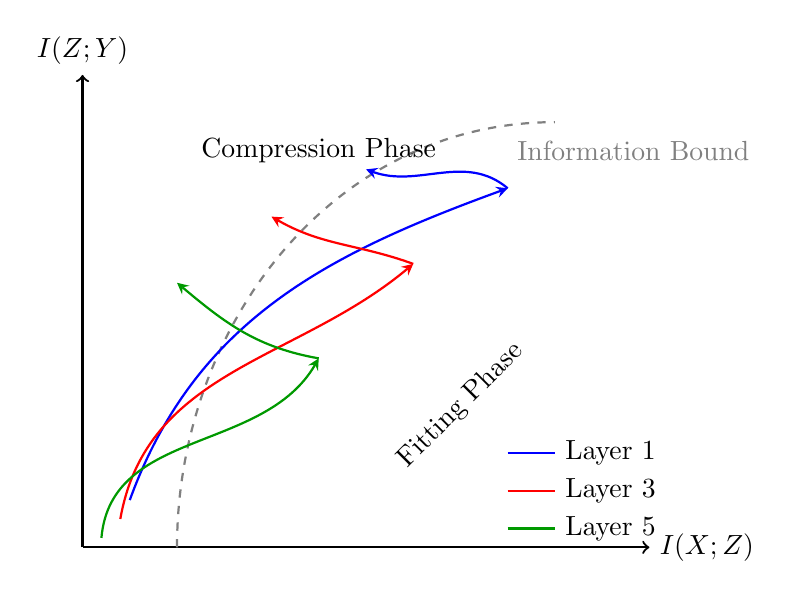
\begin{tikzpicture}[scale=1.2]
        % Axes
        \draw[->, thick] (0,0) -- (6,0) node[right] {$I(X; Z)$};
        \draw[->, thick] (0,0) -- (0,5) node[above] {$I(Z; Y)$};
        
        % Information bound curve
        \draw[thick, dashed, gray] (1,0) to[out=90, in=180] (5, 4.5);
        \node[gray, right] at (4.5, 4.2) {Information Bound};

        % Trajectories
        % Layer 1
        \draw[thick, blue, ->, >=stealth] (0.5, 0.5) to[out=70, in=200] (4.5, 3.8);
        \draw[thick, blue, ->, >=stealth] (4.5, 3.8) to[out=140, in=340] (3.0, 4.0);
        
        % Layer 3
        \draw[thick, red, ->, >=stealth] (0.4, 0.3) to[out=80, in=220] (3.5, 3.0);
        \draw[thick, red, ->, >=stealth] (3.5, 3.0) to[out=160, in=330] (2.0, 3.5);
        
        % Layer 5
        \draw[thick, green!60!black, ->, >=stealth] (0.2, 0.1) to[out=85, in=240] (2.5, 2.0);
        \draw[thick, green!60!black, ->, >=stealth] (2.5, 2.0) to[out=170, in=320] (1.0, 2.8);
        
        % Phase labels
        \node at (4.0, 1.5) [rotate=45] {Fitting Phase};
        \node at (2.5, 4.2) {Compression Phase};
        
        % Legend
        \draw[blue, thick] (4.5, 1.0) -- (5.0, 1.0) node[right, text=black] {Layer 1};
        \draw[red, thick] (4.5, 0.6) -- (5.0, 0.6) node[right, text=black] {Layer 3};
        \draw[green!60!black, thick] (4.5, 0.2) -- (5.0, 0.2) node[right, text=black] {Layer 5};
    \end{tikzpicture}
    \caption{Idealized trajectories of hidden layers in the Information Plane. Early in training, layers exhibit a fitting phase where they increase both $I(X;Z)$ and $I(Z;Y)$. As training progresses, they enter a compression phase, moving leftwards to decrease $I(X;Z)$ while maintaining $I(Z;Y)$.}
    \label{fig:info_plane}
\end{figure}

The update rule for SGD with learning rate $\eta$ and mini-batch size $B$ at iteration $t$ is defined as:
\begin{equation}
    \theta_{t+1} = \theta_t - \eta \nabla_\theta \hat{\mathcal{L}}_B(\theta_t)
\end{equation}
where $\hat{\mathcal{L}}_B(\theta) = \frac{1}{B} \sum_{i=1}^B \mathcal{L}(f_\theta(x_i), y_i)$ is the empirical loss computed over the current mini-batch drawn uniformly from the dataset $\mathcal{D}$. 

We can decompose the mini-batch gradient into the true full-batch gradient and an additive noise term:
\begin{equation}
    \nabla_\theta \hat{\mathcal{L}}_B(\theta_t) = \nabla_\theta \mathcal{L}(\theta_t) + \xi_t
\end{equation}
By the Central Limit Theorem, assuming $B$ is sufficiently large, the noise vector $\xi_t$ is approximately multivariate Gaussian with mean zero and a position-dependent covariance matrix $\Sigma(\theta_t) \approx \frac{1}{B} \text{Cov}_{x,y}[\nabla_\theta \mathcal{L}(f_\theta(x), y)]$.

This formulation allows us to model discrete SGD as a continuous-time Stochastic Differential Equation (SDE), specifically representing Langevin dynamics:
\begin{equation}
    d\theta_t = -\eta \nabla_\theta \mathcal{L}(\theta_t) dt + \sqrt{\eta \Sigma(\theta_t)} dW_t
\end{equation}
where $W_t$ represents a standard multi-dimensional Wiener process (Brownian motion). 

\subsection{The Drift-to-Diffusion Transition}

To mathematically define the boundary between the fitting and compression phases, we examine the Signal-to-Noise Ratio (SNR) of the gradients during training. The ``signal'' is the squared norm of the expected gradient drift, and the ``noise'' is given by the trace of the covariance matrix.

\begin{definition}[Signal-to-Noise Ratio of SGD]
    The gradient SNR at training time $t$ is defined as:
    \begin{equation}
        \text{SNR}(t) = \frac{\|\nabla_\theta \mathcal{L}(\theta_t)\|^2}{\frac{1}{d} \text{tr}(\Sigma(\theta_t))}
    \end{equation}
\end{definition}

\begin{figure}[htbp]
    \centering
    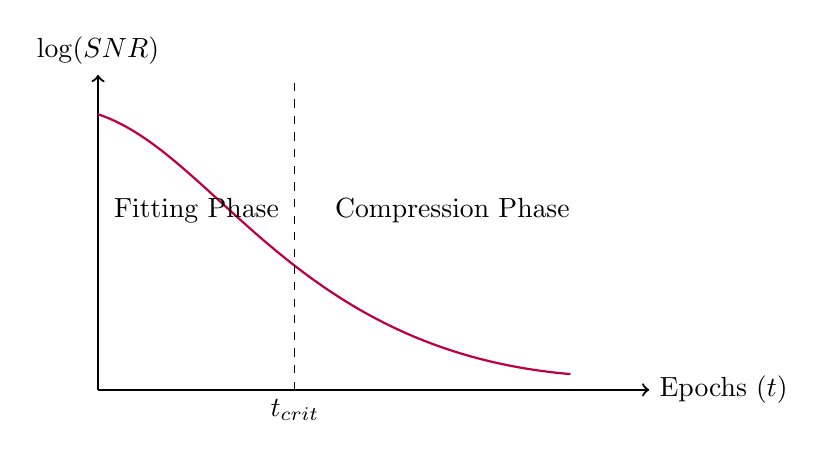
\begin{tikzpicture}[scale=1.0]
        \draw[->, thick] (0,0) -- (7,0) node[right] {Epochs ($t$)};
        \draw[->, thick] (0,0) -- (0,4) node[above] {$\log(\text{SNR})$};
        
        \draw[thick, purple] (0, 3.5) .. controls (1.5, 3.0) and (2.5, 0.5) .. (6, 0.2);
        
        \draw[dashed] (2.5, 0) -- (2.5, 4);
        \node[above] at (1.25, 2.0) {Fitting Phase};
        \node[above] at (4.5, 2.0) {Compression Phase};
        \node[below] at (2.5, 0) {$t_{\text{crit}}$};
    \end{tikzpicture}
    \caption{The transition from drift-dominated (fitting) to diffusion-dominated (compression) dynamics, marked by a critical, rapid drop in gradient SNR.}
    \label{fig:snr_drop}
\end{figure}

During the \textbf{Fitting Phase} ($t < t_{\text{crit}}$), the network parameters are far from any local minimum. The gradient magnitude is consequently large, yielding $\text{SNR} \gg 1$. The deterministic drift term $-\eta \nabla_\theta \mathcal{L}(\theta_t) dt$ dominates the SDE, rapidly driving the loss down and increasing $I(Z; Y)$.

During the \textbf{Compression Phase} ($t > t_{\text{crit}}$), the network enters a wide, flat region of the loss landscape (a ``flat minimum'') where $\nabla_\theta \mathcal{L}(\theta_t) \approx 0$. Consequently, the SNR drops exponentially. The stochastic diffusion term $\sqrt{\eta \Sigma(\theta_t)} dW_t$ now dominates the dynamics. The weights undergo a constrained random walk characterized by the noise covariance.

\subsection{Information Compression via Diffusion}

We now rigorously prove that this diffusion process inherently causes a decrease in the mutual information $I(X; Z)$. We restrict our analysis to a single hidden layer whose output is given by $Z = \phi(W X)$, where $\phi$ is a bounded, smooth activation function (such as $\tanh$ or the sigmoid function). For simplicity, we isolate the weight matrix $W$ of this specific layer, and assume the inputs $X$ are deterministic conditional on the sampled data.

\begin{theorem}[Information Compression via Weight Diffusion]
    Let $Z_t = \phi(W_t X)$ where $\phi : \mathbb{R} \to \mathbb{R}$ is a continuous, bounded activation function applied element-wise. Assume that in the compression phase, $W_t$ undergoes an isotropic diffusion process $dW_t = \sqrt{2D} d\tilde{W}_t$, where $D$ is the diffusion coefficient and $\tilde{W}_t$ is standard Brownian motion. If the marginal differential entropy $h(Z_t)$ is bounded from above, the mutual information $I(X; Z_t)$ monotonically decreases over time for sufficiently large $t$.
\end{theorem}

\begin{proof}
    By definition, the mutual information between the continuous input and the representation is:
    \begin{equation}
        I(X; Z_t) = h(Z_t) - h(Z_t | X)
    \end{equation}
    Because the activation function $\phi$ is bounded, the representation vector $Z_t$ is constrained to a compact hypercube (e.g., $[-1, 1]^k$). Therefore, by the principle of maximum entropy, the marginal differential entropy $h(Z_t)$ must be strictly bounded from above by some constant $h_{\text{max}}$.
    
    Now consider the conditional entropy $h(Z_t | X = x)$. For a fixed, constant input $x$, any randomness in $Z_t$ is induced entirely by the stochastic evolution of the weights $W_t$. 
    By applying Itô's Lemma, the diffusion of $W_t$ yields a corresponding diffusion process for the representation $Z_t$ conditional on $x$. Using a local linearization around the initial point of the diffusion $W_0$, we have:
    \begin{equation}
        Z_t \approx \phi(W_0 x) + J_x (W_t - W_0)
    \end{equation}
    where $J_x = \frac{\partial Z}{\partial W}\big|_{W=W_0}$ is the Jacobian matrix evaluated at $x$. Given that $W_t - W_0 \sim \mathcal{N}(0, 2DtI)$, the conditional distribution $P(Z_t | X=x)$ behaves asymptotically as a multivariate Gaussian with a covariance matrix $\Sigma_Z(t)$ that scales linearly with time:
    \begin{equation}
        \Sigma_Z(t) \approx 2 D t J_x J_x^T
    \end{equation}
    The differential entropy of a $k$-dimensional multivariate Gaussian is calculated as:
    \begin{equation}
        h(Z_t | X = x) = \frac{1}{2} \log \det (2 \pi e \Sigma_Z(t)) = \frac{k}{2} \log t + C(x)
    \end{equation}
    where $C(x)$ is a term dependent on the Jacobian $J_x$, the dimension $k$, and the diffusion constant $D$, but independent of time $t$.
    
    Taking the expectation over the data distribution $P(X)$ yields the overall conditional entropy:
    \begin{equation}
        h(Z_t | X) = \int P(x) h(Z_t | X=x) dx \approx \frac{k}{2} \log t + \mathbb{E}_X[C(X)]
    \end{equation}
    As $t \to \infty$ during the diffusion phase, the conditional entropy $h(Z_t | X)$ increases logarithmically without bound. 
    
    Since the marginal entropy $h(Z_t)$ remains bounded by $h_{\text{max}}$, it follows that the mutual information:
    \begin{equation}
        I(X; Z_t) = h(Z_t) - h(Z_t | X) \le h_{\text{max}} - \frac{k}{2} \log t - \mathbb{E}_X[C(X)]
    \end{equation}
    must necessarily decrease as time progresses. The persistent diffusion of the weights acts to ``blur'' the mapping from $X$ to $Z$, forcing the network to structurally forget high-resolution information about the input $X$.
\end{proof}

\subsection{Numerical Example}

To concretize this mechanism, consider a highly simplified setting: a scalar input $X \sim \mathcal{N}(0, 1)$ and a binary target $Y = \text{sgn}(X)$. We utilize a single-node hidden representation $Z = \tanh(w X)$ and a final output $\hat{Y} = \text{sgn}(v Z)$.

Suppose that at iteration $t_{100}$, marking the end of the fitting phase, the weight has reached $w = 5.0$. The mapping from $X$ to $Z$ is extremely sharp. 
\begin{align*}
    Z_{100} &= \tanh(5.0 X)
\end{align*}
Given $X=x$, $Z$ is nearly deterministic because the weights are temporarily stable. The variance of $Z|X$ is essentially zero, driving $h(Z_{100}|X) \to -\infty$ (for theoretical continuous weights) or reflecting extremely high precision. Evaluating this bounded mapping reveals that almost all information about $X$ is preserved up to the saturation regime, yielding $I(X; Z_{100}) \approx 0.95$ bits of the theoretical 1 bit maximum for this scale.

At iteration $t_{10000}$, deep in the compression phase, the weight $w$ has undergone extensive diffusion while remaining in the flat region solving the task. Its distribution might now be characterized by $w \sim \mathcal{N}(2.0, 1.5^2)$.
For a specific input, say $x=1.0$, the representation is $Z = \tanh(w)$ where $w$ is drawn from this Gaussian. The variance of $Z|X=1.0$ is now highly significant due to the variance in $w$. The conditional entropy $h(Z_{10000}|X)$ has therefore increased dramatically. A numerical integration of these distributions yields a substantially reduced mutual information $I(X; Z_{10000}) \approx 0.45$ bits. The representation has successfully compressed by shedding half a bit of information regarding the precise magnitude of $X$, while the decision boundary ($Z > 0 \implies \hat{Y} = 1$) remains perfectly intact, thus keeping $I(Z; Y)$ identical to its value in the fitting phase.

% 3. Horizon Box
\begin{horizon}
The universality and strict necessity of the compression phase remain topics of intense and active debate. While Shwartz-Ziv and Tishby observed compression robustly in networks equipped with saturating activation functions (such as $\tanh$ and sigmoid), subsequent seminal critiques (e.g., Saxe et al., 2018) fundamentally challenged the necessity of compression. They demonstrated that networks using ReLU activations often do not exhibit a distinct or visible compression phase in the Information Plane, yet these networks still generalize exceptionally well.

It is conjectured that for unbounded activation functions like ReLU, ``compression'' may not manifest as a reduction in differential entropy---which can scale arbitrarily through linear scaling of the weights---but rather through geometric clustering and a collapse in the intrinsic rank of the representations. Future work might show that the Information Plane, if augmented or normalized with invariant measures of intrinsic dimensionality, universally exhibits compression across all common architectures. A major open question is whether explicit informational compression (induced via noise) is causally responsible for robust generalization, or if it is merely a widespread epiphenomenon characteristic of stochastic optimization in high-dimensional spaces.
\end{horizon}

% 4. Summary and Exercises
\section{Summary}
\begin{itemize}
    \item The training dynamics of deep neural networks via SGD can be conceptually decomposed into a fast fitting phase and a slow compression phase when visualized on the Information Plane.
    \item This transition is characterized mathematically by a dramatic drop in the gradient Signal-to-Noise Ratio (SNR), marking a shift from drift-dominated optimization to diffusion-dominated random walks.
    \item In the compression phase, the stochastic noise inherent in SGD mini-batch sampling induces a random walk in parameter space. For bounded representations, this diffusion inherently increases the conditional entropy $h(Z|X)$ and drives a continuous decrease in the mutual information $I(X; Z)$, yielding compressed representations.
\end{itemize}

\section{Exercises}
\begin{enumerate}
    \item \textbf{Data Processing Inequality in the Plane:} Given the Markov chain sequence of layers $X \rightarrow Z_1 \rightarrow Z_2 \rightarrow Y$, formally prove that the trajectory of $Z_2$ in the Information Plane must always remain strictly below and to the left of the trajectory of $Z_1$.
    \item \textbf{Linear Networks and De Bruijn's Identity:} Consider a purely linear neural network layer defined by $Z_t = W_t X$. Show mathematically that if $W_t$ undergoes isotropic Gaussian diffusion, the conditional entropy $h(Z_t | X)$ increases, but the marginal entropy $h(Z_t)$ also increases indefinitely. Based on this result, conclude why saturating nonlinearities (or regularization) are necessary to observe true informational compression in this continuous SDE formulation.
    \item \textbf{Empirical Simulation:} Write a short Python script utilizing the \texttt{numpy} library to simulate the trajectory of a scalar weight $w_t$ undergoing SGD on the loss function $\mathcal{L}(w) = \frac{1}{4}(w^2 - 1)^2$. Inject artificial Gaussian noise to the gradient at each step. Plot the variance of $w_t$ over time after the weight reaches the local minimum at $w=1$, and observe the onset of the diffusion phase.
\end{enumerate}

% TODO-CITE: Ensure all named results are cited.

\chapter{Critiques and Nuances of the Compression Phase}

\section{The Deterministic Mapping Problem}

The Information Bottleneck (IB) theory of deep learning, particularly the influential claim that training a neural network naturally decomposes into a brief ``fitting'' phase followed by a prolonged ``compression'' phase, has sparked intense debate. In the standard narrative, as learning progresses, the network sheds irrelevant information about the input $X$ while preserving information relevant to the target $Y$. This dynamic is elegantly visualized as a trajectory in the information plane, tracing the mutual information $I(X; T)$ against $I(T; Y)$, where $T$ represents the hidden layer activations. In this view, learning is fundamentally a process of extracting a minimal sufficient statistic.

However, a fundamental critique arises when we scrutinize the nature of modern neural networks. The original experiments demonstrating the compression phase heavily relied on specific architectural choices---notably, the use of saturating activation functions like $\tanh$, and the estimation of mutual information via discretization (binning) of the hidden activations. When researchers attempted to replicate these findings using the ubiquitous Rectified Linear Unit (ReLU) and non-binned estimators, the crisp picture of compression began to blur. Networks constructed with ReLU activations did not seem to exhibit a measurable decrease in $I(X; T)$ during the later epochs of training, casting doubt on the universality of the compression phase.

The most profound theoretical critique centers on the definition of mutual information itself in deterministic systems. A standard feedforward neural network computes a deterministic function of its input. If the input $X$ is a continuous random variable and the mapping from $X$ to $T$ is deterministic and sufficiently well-behaved, the mutual information $I(X; T)$ is strictly infinite. This mathematical reality poses a severe challenge to the empirical observation of a changing $I(X; T)$. If the true mutual information is vacuous or infinite, what exactly were the original IB experiments measuring?

This chapter dissects these critiques. We begin by formalizing the pathologies of mutual information in deterministic networks, showing that what appears to be information compression may in fact be an artifact of binning or the saturation of activation functions. We then explore alternative interpretations, such as geometric clustering, which suggest that while the \emph{informational} volume might not decrease in a well-defined Shannon sense, the \emph{geometric} volume of the representations certainly does. By resolving these nuances, we aim to preserve the powerful intuition of the Information Bottleneck while grounding it in mathematically rigorous footing that applies to the networks used in practice today.

\section{Mathematical Pathologies of Mutual Information}

\subsection{Infinite Mutual Information in Continuous Deterministic Systems}

To understand the critique of the compression phase, we must formally evaluate $I(X; T)$ when $T = f_\theta(X)$ is a deterministic transformation parameterized by $\theta$.

\begin{theorem}[Infinite Mutual Information in Deterministic Networks]
\label{thm:infinite_mi}
Let $X \in \mathbb{R}^d$ be a continuous random variable with a strictly positive probability density function on its support. Let $f_\theta: \mathbb{R}^d \to \mathbb{R}^m$ be a deterministic, piecewise continuously differentiable function representing a neural network layer, and let $T = f_\theta(X)$. If $f_\theta$ is injective on any open set of the support of $X$, then the mutual information $I(X; T)$ is infinite.
\end{theorem}

\begin{proof}
Recall the definition of mutual information for continuous random variables:
\[
I(X; T) = h(T) - h(T | X)
\]
Since $T$ is completely determined by $X$, the conditional distribution $p(t | x)$ is a Dirac delta function $\delta(t - f_\theta(x))$. The differential entropy of a Dirac delta function is negatively infinite:
\[
h(T | X) = \int p(x) \int \delta(t - f_\theta(x)) \log \frac{1}{\delta(t - f_\theta(x))} \, dt \, dx \to -\infty
\]
Assuming the marginal differential entropy $h(T)$ is finite (which holds if $T$ has a bounded density), we are subtracting a negatively infinite quantity, yielding $I(X; T) = \infty$.

Alternatively, evaluating the Kullback-Leibler divergence between the joint and the product of marginals:
\[
I(X; T) = D_{\text{KL}}(P(X, T) \parallel P(X)P(T)) = \int \int p(x, t) \log \frac{p(x, t)}{p(x)p(t)} \, dx \, dt
\]
The joint distribution $p(x, t)$ is singular with respect to the product distribution $p(x)p(t)$. Specifically, all the probability mass of $p(x,t)$ lies on the lower-dimensional manifold $t = f_\theta(x)$, which has measure zero in the product space $\mathbb{R}^d \times \mathbb{R}^m$. Therefore, the Radon-Nikodym derivative does not exist, and the divergence evaluates to $+\infty$.
\end{proof}

This theorem highlights a critical flaw: for deterministic networks without injected noise, the quantity $I(X; T)$ is a mathematical constant (infinity) and cannot dynamically change during training. The observed ``compression'' must therefore stem from the estimation procedure rather than the true Shannon mutual information.

\begin{figure}[htbp]
\centering
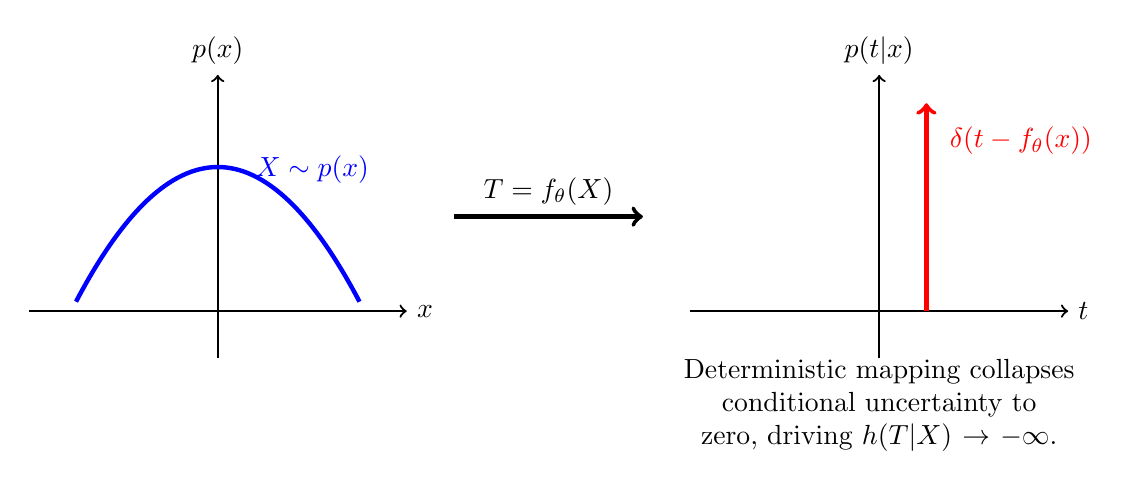
\begin{tikzpicture}[scale=1.2]
    % Axes for X
    \draw[->, thick] (-2,0) -- (2,0) node[right] {$x$};
    \draw[->, thick] (0,-0.5) -- (0,2.5) node[above] {$p(x)$};
    % PDF of X
    \draw[ultra thick, blue] (-1.5,0.1) .. controls (-0.5,2) and (0.5,2) .. (1.5,0.1);
    \node[blue] at (1,1.5) {$X \sim p(x)$};

    % Arrow for deterministic function
    \draw[->, ultra thick] (2.5, 1) -- (4.5, 1) node[midway, above] {$T = f_\theta(X)$};

    % Axes for T
    \draw[->, thick] (5,0) -- (9,0) node[right] {$t$};
    \draw[->, thick] (7,-0.5) -- (7,2.5) node[above] {$p(t|x)$};
    
    % PDF of T - Dirac delta
    \draw[ultra thick, red, ->] (7.5,0) -- (7.5,2.2);
    \node[red] at (8.5,1.8) {$\delta(t - f_\theta(x))$};
    
    \node[align=center, text width=5cm] at (7, -1) {Deterministic mapping collapses   conditional uncertainty to zero,   driving $h(T|X) \to -\infty$.};
\end{tikzpicture}
\caption{In a deterministic neural network, the mapping from the input $X$ to the representation $T$ is absolute. The conditional probability $p(t|x)$ is a Dirac delta, making the mutual information strictly infinite.}
\label{fig:deterministic_mapping}
\end{figure}

\subsection{The Illusion of Compression via Binning}

If the true mutual information is infinite, why did early empirical studies observe a distinct compression phase? The answer lies in the estimation method. To compute $I(X; T)$ computationally, early works partitioned the continuous range of $T$ into discrete bins, essentially measuring the information of a quantized variable, $\hat{T}$.

\begin{theorem}[Binned Mutual Information]
Let the range of $T \in \mathbb{R}^m$ be partitioned into uniform hypercubical bins of side length $\Delta$. Let $\hat{T} = [T]_\Delta$ be the discrete binned variable. As $\Delta \to 0$, the mutual information of the binned representation satisfies:
\[
I(X; \hat{T}) \approx H(\hat{T}) \approx h(T) - m \log \Delta
\]
assuming $T$ has a continuous and bounded probability density function.
\end{theorem}

\begin{proof}
Because $T$ is a deterministic function of $X$, the binned variable $\hat{T}$ is also entirely determined by $X$. Therefore, the discrete conditional entropy $H(\hat{T} | X) = 0$. 
It follows directly that $I(X; \hat{T}) = H(\hat{T}) - H(\hat{T} | X) = H(\hat{T})$.
From standard information theory, the discrete entropy of a finely quantized continuous variable is related to its differential entropy by:
\[
H(\hat{T}) = h(T) - \log(\Delta^m) + \mathcal{O}(\Delta) = h(T) - m \log \Delta + \mathcal{O}(\Delta)
\]
Thus, for sufficiently small $\Delta$, $I(X; \hat{T}) \approx h(T) - m \log \Delta$.
\end{proof}

This result is revealing. The measured mutual information $I(X; \hat{T})$ is essentially tracking the differential entropy $h(T)$ of the hidden representations, shifted by a constant that depends arbitrarily on the bin size $\Delta$. The perceived ``compression of information from $X$'' is actually just a reduction in the differential entropy of $T$.

\subsection{Numerical Example: Saturation and Differential Entropy}

Why would the differential entropy $h(T)$ decrease during training? Consider a single hidden neuron with a $\tanh$ activation function: $T = \tanh(w X)$, where $w \in \mathbb{R}$ is the learned weight. Let the input $X \sim \mathcal{N}(0, 1)$.

The differential entropy of $T$ can be calculated using the change of variables formula:
\[
h(T) = h(X) + \mathbb{E}_{X}\left[ \log \left| \frac{dT}{dX} \right| \right]
\]
The derivative of the mapping is $\frac{dT}{dX} = w (1 - \tanh^2(wX))$. Therefore:
\[
h(T) = \frac{1}{2}\log(2\pi e) + \mathbb{E}_{X}\left[ \log |w| + \log(1 - \tanh^2(wX)) \right]
\]

During the ``fitting'' phase, the weight magnitude $|w|$ grows from near-zero to perfectly classify the training data. As $|w| \to \infty$, the pre-activation $wX$ takes on large values, pushing the outputs into the saturating tails of the $\tanh$ function. In these tails, $(1 - \tanh^2(wX)) \to 0$, causing the logarithmic term to plummet towards $-\infty$. 

Consequently, $h(T)$ decreases drastically. When this space is binned, the discrete entropy $H(\hat{T})$ drops because the vast majority of points are tightly clustered into the two outermost bins near $-1$ and $+1$. Thus, the compression phase observed in these networks is primarily a measure of \emph{activation saturation}. If a non-saturating activation function like ReLU is used, where the derivative is piecewise constant, this specific form of entropy reduction does not occur, explaining why ReLU networks do not exhibit the same binned compression dynamics.

\section{Geometric Compression and Clustering}

If the Shannon mutual information is pathological for deterministic networks, what is the correct formalization of the compression phenomenon? A compelling alternative argues that compression occurs \emph{geometrically} rather than information-theoretically.

During training, neural networks learn to map inputs belonging to the same class into tight clusters in the latent space $\mathcal{T}$, while pushing different classes apart. This reduces the \emph{geometric volume} occupied by the representations of a single class, achieving the goal of discarding irrelevant intraclass variance.

\begin{definition}[Class Geometric Volume]
Let $\mathcal{D}_k = \{x_i \in \mathcal{D} \mid y_i = k\}$ be the set of inputs belonging to class $k$. Assuming the representations $T$ of class $k$ have a covariance matrix $\Sigma_k^{(T)}$, the geometric volume of class $k$ in the representation space is proportional to:
\[
V_k(T) = \sqrt{\det(\Sigma_k^{(T)})}
\]
\end{definition}

\begin{proposition}[Geometric Compression Implies Entropy Reduction]
If the within-class covariance $\Sigma_k^{(T)}$ shrinks uniformly by a factor $\alpha < 1$ such that the new covariance is $\tilde{\Sigma}_k^{(T)} = \alpha^2 \Sigma_k^{(T)}$, the class-conditional differential entropy $h(T|Y=k)$ decreases by $m \log \alpha$, where $m$ is the dimensionality of $T$.
\end{proposition}

\begin{proof}
Assuming the representations within a class are approximately Gaussian, $T|Y=k \sim \mathcal{N}(\mu_k, \Sigma_k^{(T)})$, the conditional differential entropy is:
\[
h(T|Y=k) = \frac{1}{2} \log \det(2\pi e \Sigma_k^{(T)})
\]
If the covariance scales by $\alpha^2$, the determinant scales by $(\alpha^2)^m = \alpha^{2m}$. Thus, the new entropy is:
\begin{align*}
\tilde{h}(T|Y=k) &= \frac{1}{2} \log \left( \det(2\pi e \alpha^2 \Sigma_k^{(T)}) \right) \\
&= \frac{1}{2} \log \left( \alpha^{2m} \det(2\pi e \Sigma_k^{(T)}) \right) \\
&= \frac{1}{2} \left( 2m \log \alpha + \log \det(2\pi e \Sigma_k^{(T)}) \right) \\
&= h(T|Y=k) + m \log \alpha
\end{align*}
Since $\alpha < 1$, the term $\log \alpha$ is strictly negative, proving that geometric compression strictly reduces conditional differential entropy.
\end{proof}

This geometric perspective aligns perfectly with the goal of invariant representations: the network compresses nuisance variations (shrinking $V_k(T)$) while maximizing the distance between class means. It does not require binning and applies equally to ReLU networks, offering a more robust interpretation of the bottleneck effect.

\begin{figure}[htbp]
\centering
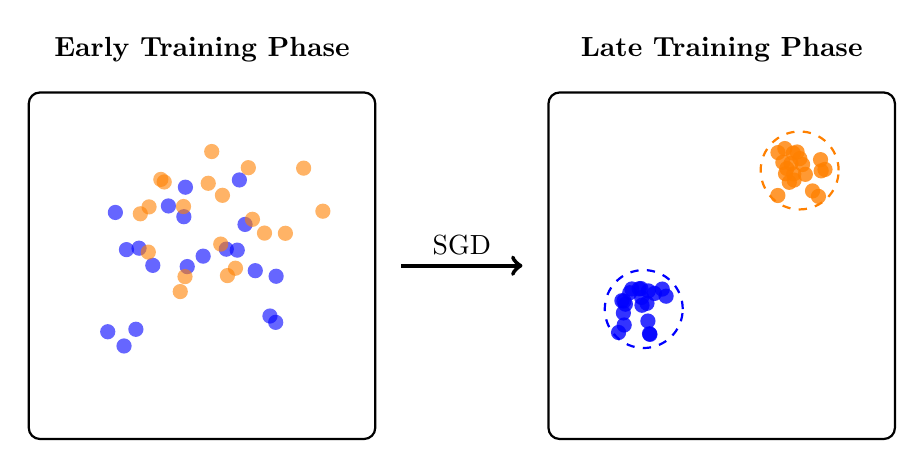
\begin{tikzpicture}[scale=1.1]
    % Initial phase
    \node at (2, 4.5) {\textbf{Early Training Phase}};
    \draw[thick, rounded corners] (0,0) rectangle (4,4);
    
    % Class 1 scattered
    \foreach \i in {1,...,20} {
        \fill[blue, opacity=0.6] (0.8+rnd*2.2, 0.8+rnd*2.2) circle (2.5pt);
    }
    % Class 2 scattered
    \foreach \i in {1,...,20} {
        \fill[orange, opacity=0.6] (1.2+rnd*2.2, 1.2+rnd*2.2) circle (2.5pt);
    }
    
    \draw[->, ultra thick] (4.3, 2) -- (5.7, 2) node[midway, above] {SGD};

    % Late phase
    \node at (8, 4.5) {\textbf{Late Training Phase}};
    \draw[thick, rounded corners] (6,0) rectangle (10,4);
    
    % Class 1 clustered
    \foreach \i in {1,...,20} {
        \fill[blue, opacity=0.8] (6.8+rnd*0.6, 1.2+rnd*0.6) circle (2.5pt);
    }
    % Class 2 clustered
    \foreach \i in {1,...,20} {
        \fill[orange, opacity=0.8] (8.6+rnd*0.6, 2.8+rnd*0.6) circle (2.5pt);
    }
    
    % Ellipses showing volume
    \draw[blue, thick, dashed] (7.1, 1.5) ellipse (0.45 and 0.45);
    \draw[orange, thick, dashed] (8.9, 3.1) ellipse (0.45 and 0.45);

\end{tikzpicture}
\caption{Geometric compression in the representation space $\mathcal{T}$. During the fitting phase, class distributions are heavily entangled with high geometric volume. As training progresses, the network geometrically compresses samples of the same class into tight clusters, reducing $V_k(T)$ while maximizing inter-class margins.}
\label{fig:geometric_compression}
\end{figure}

\begin{horizon}
While the pathology of deterministic mappings invalidates a naive application of the Shannon Information Bottleneck to standard networks, the fundamental intuition remains profoundly compelling. It is conjectured that there exists a generalized ``information-like'' metric that naturally unifies the deterministic and stochastic regimes, capturing the essence of compression without falling prey to infinite singularities. 

Future work might show that replacing Shannon entropy with rigorous topological measures---such as the intrinsic fractal dimension of the data manifold or optimal transport distances between conditional class distributions---yields a generalized IB principle. Such a principle would ideally track generalization cleanly, invariant to whether the network utilizes $\tanh$ or ReLU activations, and without requiring arbitrary binning strategies.

An exciting open question is whether the implicit regularization of stochastic gradient descent inherently minimizes this yet-to-be-defined geometric compression metric. If it is conjectured that the noise in SGD acts as a geometric smoother, driving the representations toward minimal-volume states, this could finally explain the generalization capabilities of heavily overparameterized models through a unified, bottleneck-like mechanism.
\end{horizon}

\section{Summary}
In this chapter, we critiqued the standard Information Bottleneck theory applied to deep learning. We demonstrated that for continuous, deterministic neural networks, the mutual information $I(X; T)$ between the input and hidden layers is technically infinite. Consequently, the widely observed ``compression phase'' in early literature is largely an artifact of two phenomena: the discretization of continuous representations via arbitrary binning, and the shrinking differential entropy caused by saturating activation functions like $\tanh$. 

To salvage the core intuition of the Information Bottleneck, we shifted our perspective from strict Shannon information to geometric clustering. We proved that as the network maps data belonging to the same class into dense regions, the geometric volume and conditional differential entropy of the representations decrease. This geometric viewpoint provides a rigorous framework for understanding how networks abstract away nuisance variables without succumbing to the mathematical pathologies of deterministic mutual information.

\section*{Exercises}
\begin{enumerate}
    \item \textbf{Infinite Information:} Construct a simple 1D continuous random variable $X \sim U(0, 1)$ and a deterministic function $T = 2X$. Calculate $h(T)$. Explain mathematically why $I(X; T) = \infty$ despite the mapping being a simple linear scaling.
    \item \textbf{Saturating Activations:} Let $X \sim \mathcal{N}(0, 1)$ and $T = \sigma(wX)$, where $\sigma(z) = 1/(1+e^{-z})$ is the sigmoid function. Derive an expression for the differential entropy $h(T)$ as a function of the weight $w$. Show analytically that $h(T) \to -\infty$ as $w \to \infty$.
    \item \textbf{ReLU and Binning:} Repeat the empirical binning analysis for a ReLU activation, $T = \max(0, wX)$. Assuming $X \sim \mathcal{N}(0, 1)$, what happens to the binned entropy $H(\hat{T})$ as $w$ increases? Does it show a compression phase similar to saturating activations?
    \item \textbf{Geometric Volume:} Prove that applying an orthogonal weight matrix $W$ (where $W^\top W = I$) to a hidden representation preserves its class-conditional geometric volume $V_k(T)$. 
    \item \textbf{Noise Injection:} Suppose we modify a deterministic network by adding Gaussian noise: $T = f_\theta(X) + \epsilon$, where $\epsilon \sim \mathcal{N}(0, \sigma^2 I)$. Show that $I(X; T)$ is now strictly finite, and express it in terms of $h(T)$ and $\sigma$.
\end{enumerate}

% TODO-CITE: Ensure all named results are cited.


\part{Variational Inference and Autoencoders}
\chapter{The Evidence Lower Bound (ELBO)}
\label{chap:elbo}

\section{The Problem of Intractable Inference}

The ambition of deep generative modeling is to discover the hidden, low-dimensional factors that give rise to the high-dimensional data we observe in the real world. From images of human faces to the complex waveforms of human speech, we postulate the existence of a latent variable $z \in \mathcal{Z}$ that fundamentally describes an observation $x \in \mathcal{X}$. The generative process is governed by a joint probability distribution $p_\theta(x, z) = p_\theta(x|z)p(z)$, where $p(z)$ is a prior distribution over the latent space and $p_\theta(x|z)$ is the likelihood function parameterized by a powerful function approximator, typically a deep neural network with weights $\theta$.

If we wish to learn the parameters $\theta$ that best explain our dataset $\mathcal{D}$, the principle of maximum likelihood dictates that we should maximize the marginal likelihood, also known as the \textit{evidence}. The evidence is obtained by marginalizing out all possible latent configurations:
\begin{equation}
    p_\theta(x) = \int p_\theta(x|z) p(z) \, dz.
\end{equation}
In all but the simplest linear-Gaussian models, this integral is analytically intractable. The latent space $\mathcal{Z}$ is typically high-dimensional, rendering numerical quadrature impossible. Brute-force Monte Carlo integration is equally hopeless due to the curse of dimensionality; for complex models, the vast majority of sampled $z$ vectors will produce a near-zero likelihood $p_\theta(x|z)$, meaning the variance of naive sampling estimates is astronomically high.

A related, and equally insurmountable, challenge is probabilistic inference. If we observe a datum $x$, what were the specific latent factors $z$ that generated it? Bayes' theorem provides the formal answer via the posterior distribution:
\begin{equation}
    p_\theta(z|x) = \frac{p_\theta(x|z) p(z)}{p_\theta(x)}.
\end{equation}
Because the denominator is the intractable evidence $p_\theta(x)$, evaluating the true posterior $p_\theta(z|x)$ is correspondingly intractable. We are confronted with a chicken-and-egg problem: we need the posterior to understand the internal representations of our data and to properly update our parameters, but we cannot compute the posterior without evaluating the very integral we cannot solve. Without access to the posterior, we cannot apply the Expectation-Maximization (EM) algorithm or any standard likelihood-based optimization technique.

The elegant resolution to this profound mathematical impasse is \textit{variational inference}. Instead of attempting to compute the exact posterior $p_\theta(z|x)$ via brute-force integration, we introduce a new, completely tractable distribution $q_\phi(z|x)$. This distribution—often called the \textit{variational distribution}, \textit{inference model}, or simply the \textit{encoder}—is parameterized by its own set of distinct parameters $\phi$ (such as the weights of a secondary neural network). We then profoundly reframe the problem of Bayesian inference as a problem of pure optimization: we seek to find the parameters $\phi$ that make our tractable $q_\phi(z|x)$ as close as possible to the intractable true posterior $p_\theta(z|x)$.

This shift from integration to optimization is the cornerstone of modern approximate inference. By constructing a lower bound on the log-evidence—the Evidence Lower Bound (ELBO)—we create a surrogate objective function that can be efficiently, jointly optimized with respect to both the generative parameters $\theta$ and the variational parameters $\phi$ using standard stochastic gradient descent. The ELBO not only provides a mathematically rigorous, tractable proxy for maximum likelihood estimation, but it also elegantly bridges the disciplines of information theory, Bayesian statistics, and deep representation learning.

\section{Derivation of the Evidence Lower Bound}

We now formally derive the ELBO. The mathematical machinery relies on the foundational concepts of Kullback-Leibler (KL) divergence and Jensen's inequality. 

\begin{theorem}[The ELBO Decomposition]
\label{thm:elbo_decomp}
Let $p_\theta(x, z)$ be a generative model with latent variables $z$ and observations $x$. Let $q_\phi(z|x)$ be an arbitrary conditional distribution over the latent variables given the observations, with support encompassing that of $p_\theta(z|x)$. The log-marginal likelihood $\log p_\theta(x)$ can be uniquely decomposed as:
\begin{equation}
    \log p_\theta(x) = \mathrm{ELBO}(x; \theta, \phi) + D_{\mathrm{KL}}(q_\phi(z|x) \parallel p_\theta(z|x)),
\end{equation}
where the Evidence Lower Bound (ELBO) is defined as:
\begin{equation}
    \mathrm{ELBO}(x; \theta, \phi) \triangleq \mathbb{E}_{q_\phi(z|x)}\left[ \log \frac{p_\theta(x, z)}{q_\phi(z|x)} \right].
\end{equation}
\end{theorem}

\begin{proof}
By definition of the marginal likelihood, we can write $\log p_\theta(x)$ as the expectation of a constant with respect to the distribution $q_\phi(z|x)$, since $p_\theta(x)$ does not depend on $z$:
\begin{equation}
    \log p_\theta(x) = \mathbb{E}_{q_\phi(z|x)}[ \log p_\theta(x) ].
\end{equation}
Using Bayes' theorem, we can expand the marginal likelihood inside the expectation as $p_\theta(x) = \frac{p_\theta(x, z)}{p_\theta(z|x)}$:
\begin{equation}
    \log p_\theta(x) = \mathbb{E}_{q_\phi(z|x)}\left[ \log \frac{p_\theta(x, z)}{p_\theta(z|x)} \right].
\end{equation}
We then multiply the numerator and denominator inside the logarithm by the variational distribution $q_\phi(z|x)$:
\begin{equation}
    \log p_\theta(x) = \mathbb{E}_{q_\phi(z|x)}\left[ \log \left( \frac{p_\theta(x, z)}{q_\phi(z|x)} \frac{q_\phi(z|x)}{p_\theta(z|x)} \right) \right].
\end{equation}
Using the properties of logarithms, we separate this into two expectations:
\begin{equation}
    \log p_\theta(x) = \mathbb{E}_{q_\phi(z|x)}\left[ \log \frac{p_\theta(x, z)}{q_\phi(z|x)} \right] + \mathbb{E}_{q_\phi(z|x)}\left[ \log \frac{q_\phi(z|x)}{p_\theta(z|x)} \right].
\end{equation}
The first term is precisely the definition of the ELBO. The second term is, by definition, the Kullback-Leibler divergence from the variational distribution to the true posterior. Thus, we arrive at the result:
\begin{equation}
    \log p_\theta(x) = \mathrm{ELBO}(x; \theta, \phi) + D_{\mathrm{KL}}(q_\phi(z|x) \parallel p_\theta(z|x)).
\end{equation}
\end{proof}

\begin{corollary}[The Lower Bound Property]
Because the Kullback-Leibler divergence is non-negative for any two valid probability distributions (a consequence of Gibbs' inequality), i.e., $D_{\mathrm{KL}}(P \parallel Q) \geq 0$, it strictly follows that:
\begin{equation}
    \log p_\theta(x) \geq \mathrm{ELBO}(x; \theta, \phi).
\end{equation}
The bound is tight (holds with exact equality) if and only if $q_\phi(z|x) = p_\theta(z|x)$ almost everywhere, which occurs when the variational distribution perfectly matches the true posterior, implying $D_{\mathrm{KL}}(q_\phi(z|x) \parallel p_\theta(z|x)) = 0$.
\end{corollary}

An alternative, perhaps more direct, derivation of the lower bound property invokes Jensen's inequality applied to the concave logarithm function.

\begin{proof}[Alternative Proof via Jensen's Inequality]
We begin with the definition of the log-marginal likelihood:
\begin{equation}
    \log p_\theta(x) = \log \int p_\theta(x, z) \, dz.
\end{equation}
We multiply and divide the integrand by the variational distribution $q_\phi(z|x)$:
\begin{equation}
    \log p_\theta(x) = \log \int q_\phi(z|x) \frac{p_\theta(x, z)}{q_\phi(z|x)} \, dz = \log \mathbb{E}_{q_\phi(z|x)}\left[ \frac{p_\theta(x, z)}{q_\phi(z|x)} \right].
\end{equation}
Because the logarithm is a strictly concave function, we apply Jensen's inequality ($\log \mathbb{E}[Y] \geq \mathbb{E}[\log Y]$):
\begin{equation}
    \log p_\theta(x) \geq \mathbb{E}_{q_\phi(z|x)}\left[ \log \frac{p_\theta(x, z)}{q_\phi(z|x)} \right] = \mathrm{ELBO}(x; \theta, \phi).
\end{equation}
\end{proof}

This decomposition elegantly illustrates the dual nature of optimizing the ELBO. Because $\log p_\theta(x)$ depends only on $\theta$ and is independent of $\phi$, maximizing the ELBO with respect to $\phi$ strictly minimizes the KL divergence $D_{\mathrm{KL}}(q_\phi(z|x) \parallel p_\theta(z|x))$. In doing so, it forces our approximate posterior to better represent the true posterior. Conversely, maximizing the ELBO with respect to $\theta$ pushes up the lower bound, thereby implicitly maximizing the log-evidence of the data itself.

\begin{figure}[htbp]
\centering
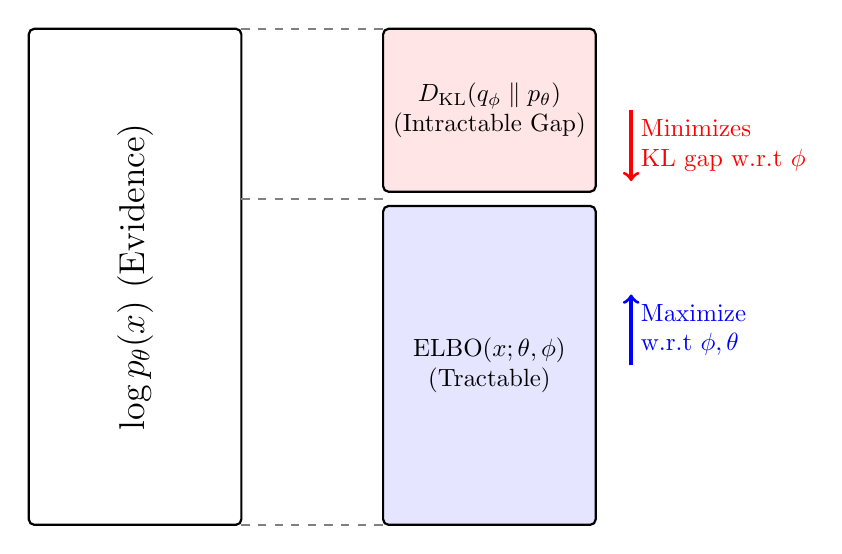
\begin{tikzpicture}[scale=0.9, every node/.style={transform shape}]
    % Total log p(x) block
    \draw[thick, rounded corners=2pt] (0,0) rectangle (3, 7);
    \node[rotate=90, font=\Large] at (1.5, 3.5) {$\log p_\theta(x)$ (Evidence)};
    
    % ELBO block
    \draw[fill=blue!10, thick, rounded corners=2pt] (5,0) rectangle (8, 4.5);
    \node[align=center] at (6.5, 2.25) {$\mathrm{ELBO}(x; \theta, \phi)$ \\ (Tractable)};
    
    % KL block
    \draw[fill=red!10, thick, rounded corners=2pt] (5,4.7) rectangle (8, 7);
    \node[align=center] at (6.5, 5.85) {$D_{\mathrm{KL}}(q_\phi \parallel p_\theta)$ \\ (Intractable Gap)};
    
    % Connections
    \draw[dashed, gray, thick] (3,0) -- (5,0);
    \draw[dashed, gray, thick] (3,7) -- (5,7);
    \draw[dashed, gray, thick] (3,4.6) -- (5,4.6);
    
    % Arrows showing optimization
    \draw[->, very thick, blue] (8.5, 2.25) -- ++(0, 1) node[midway, right, align=left] {Maximize \\ w.r.t $\phi, \theta$};
    \draw[->, very thick, red] (8.5, 5.85) -- ++(0, -1) node[midway, right, align=left] {Minimizes \\ KL gap w.r.t $\phi$};
\end{tikzpicture}
\caption{The Geometry of the Evidence Lower Bound. The log-evidence $\log p_\theta(x)$ is a fixed quantity for a given $\theta$. By maximizing the ELBO with respect to the variational parameters $\phi$, we squeeze the strictly positive KL divergence gap, tightening the bound.}
\label{fig:elbo_geometry}
\end{figure}

\section{Information-Theoretic Interpretation of the ELBO}

The ELBO can be algebraically rearranged into a form that exposes its profound connection to information theory and autoencoding. By expanding the joint distribution $p_\theta(x, z) = p_\theta(x|z)p(z)$, we rewrite the ELBO as:
\begin{align}
    \mathrm{ELBO}(x; \theta, \phi) &= \mathbb{E}_{q_\phi(z|x)}\left[ \log \frac{p_\theta(x|z)p(z)}{q_\phi(z|x)} \right] \nonumber \\
    &= \mathbb{E}_{q_\phi(z|x)}[ \log p_\theta(x|z) ] + \mathbb{E}_{q_\phi(z|x)}\left[ \log \frac{p(z)}{q_\phi(z|x)} \right] \nonumber \\
    &= \mathbb{E}_{q_\phi(z|x)}[ \log p_\theta(x|z) ] - D_{\mathrm{KL}}(q_\phi(z|x) \parallel p(z)).
\end{align}

This formulation reveals the ELBO as a principled trade-off between two distinct information-theoretic forces:
\begin{enumerate}
    \item \textbf{Reconstruction Likelihood:} The term $\mathbb{E}_{q_\phi(z|x)}[ \log p_\theta(x|z) ]$ measures how well the decoder $p_\theta(x|z)$ can reconstruct the data $x$ given latent representations $z$ sampled from the encoder $q_\phi(z|x)$. This acts as a data-fitting or distortion-minimizing term.
    \item \textbf{Complexity Penalty (Regularization):} The term $D_{\mathrm{KL}}(q_\phi(z|x) \parallel p(z))$ quantifies the information cost of encoding the data. It measures how much the variational posterior deviates from the uninformative prior $p(z)$. From an information-theoretic lens, this is the rate of information transmitted from the data to the latent space; penalizing it strictly limits the capacity of the latent channel, thereby compressing the representation.
\end{enumerate}

This tension perfectly mirrors the Information Bottleneck principle discussed earlier in Chapter 8. We are maximizing the mutual information between the latent representation and the observation (by ensuring the latents can decode the observation) while minimizing the information the latents carry about the observation beyond what is strictly necessary (by forcing the posterior to match a naive prior).

\begin{figure}[htbp]
\centering
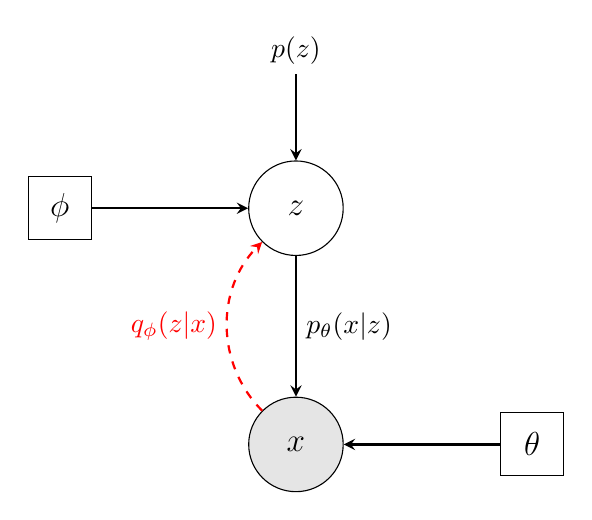
\begin{tikzpicture}[
    obs/.style={circle, draw, fill=gray!20, minimum size=1.2cm, font=\large},
    lat/.style={circle, draw, minimum size=1.2cm, font=\large},
    param/.style={rectangle, draw, minimum size=0.8cm, font=\large},
    arr/.style={-stealth, thick},
    var_arr/.style={-stealth, thick, dashed, red}
]
    % Nodes using absolute coordinates for reliability
    \node[lat] (z) at (0, 3) {$z$};
    \node[obs] (x) at (0, 0) {$x$};
    \node[param] (phi) at (-3, 3) {$\phi$};
    \node[param] (theta) at (3, 0) {$\theta$};
    \node (prior) at (0, 5) {$p(z)$};
    
    % Generative paths
    \draw[arr] (prior) -- (z);
    \draw[arr] (z) -- node[right, pos=0.5] {$p_\theta(x|z)$} (x);
    \draw[arr] (theta) -- (x);
    
    % Variational paths
    \draw[var_arr] (x) to[bend left=45] node[left, pos=0.5] {$q_\phi(z|x)$} (z);
    \draw[arr] (phi) -- (z);
\end{tikzpicture}
\caption{Graphical model depicting the generative process and the variational inference model. Solid black lines represent the generative model parameters $\theta$ dictating the mapping from latents to observations. The dashed red line represents the parameterized encoder $\phi$ actively inferring latents from data.}
\label{fig:elbo_graphical}
\end{figure}

\section{A Tractable Numerical Example: Linear Gaussian Model}

To concretely demonstrate the internal mechanics of the ELBO, we turn to a scenario where the integrals \textit{are} entirely tractable, allowing us to explicitly calculate both the true posterior and the KL divergence gap. Let the true generative model be a scalar linear Gaussian:
\begin{align}
    \text{Prior:} \quad & p(z) = \mathcal{N}(z; 0, 1) \\
    \text{Likelihood:} \quad & p_\theta(x|z) = \mathcal{N}(x; z, \sigma^2).
\end{align}
Because both the prior and likelihood are Gaussian and their relationship is linear, the true posterior and the marginal likelihood are analytically available in closed form. By completing the square on the exponent, the true posterior is derived as:
\begin{equation}
    p_\theta(z|x) = \mathcal{N}\left(z; \frac{x}{1+\sigma^2}, \frac{\sigma^2}{1+\sigma^2}\right),
\end{equation}
and the true marginal likelihood is:
\begin{equation}
    p_\theta(x) = \mathcal{N}(x; 0, 1+\sigma^2).
\end{equation}

Now, assume we forget we know the exact posterior and attempt to perform variational inference. We propose a variational family of isotropic Gaussians parameterized by a mean $\mu_\phi$ and variance $s_\phi^2$:
\begin{equation}
    q_\phi(z|x) = \mathcal{N}(z; \mu_\phi, s_\phi^2).
\end{equation}
We wish to compute the ELBO for a fixed observation $x$:
\begin{equation}
    \mathrm{ELBO} = \mathbb{E}_{q_\phi}[ \log p_\theta(x|z) ] - D_{\mathrm{KL}}(q_\phi(z|x) \parallel p(z)).
\end{equation}
The KL divergence between two univariate Gaussians has a known closed form:
\begin{equation}
    D_{\mathrm{KL}}(\mathcal{N}(\mu_\phi, s_\phi^2) \parallel \mathcal{N}(0, 1)) = \frac{1}{2}\left( s_\phi^2 + \mu_\phi^2 - 1 - \log(s_\phi^2) \right).
\end{equation}
The expected log-likelihood under $q_\phi$ evaluates to:
\begin{align}
    \mathbb{E}_{q_\phi}[ \log \mathcal{N}(x; z, \sigma^2) ] &= \mathbb{E}_{q_\phi}\left[ -\frac{1}{2}\log(2\pi\sigma^2) - \frac{(x-z)^2}{2\sigma^2} \right] \nonumber \\
    &= -\frac{1}{2}\log(2\pi\sigma^2) - \frac{1}{2\sigma^2} \mathbb{E}_{q_\phi}[ (x-z)^2 ].
\end{align}
Using the variance identity $\mathbb{E}[ (x-z)^2 ] = (x - \mathbb{E}[z])^2 + \mathrm{Var}(z)$, we get:
\begin{equation}
    \mathbb{E}_{q_\phi}[ (x-z)^2 ] = (x - \mu_\phi)^2 + s_\phi^2.
\end{equation}
Substituting these into the original ELBO expression yields the fully expanded objective:
\begin{equation}
    \mathrm{ELBO}(\mu_\phi, s_\phi^2) = -\frac{1}{2}\log(2\pi\sigma^2) - \frac{(x - \mu_\phi)^2 + s_\phi^2}{2\sigma^2} - \frac{1}{2}\left( s_\phi^2 + \mu_\phi^2 - 1 - \log(s_\phi^2) \right).
\end{equation}
To maximize this lower bound, we analytically find the stationary points with respect to the variational parameters $\mu_\phi$ and $s_\phi^2$:
\begin{align}
    \frac{\partial \mathrm{ELBO}}{\partial \mu_\phi} &= \frac{x - \mu_\phi}{\sigma^2} - \mu_\phi = 0 \implies \mu_\phi^* = \frac{x}{1+\sigma^2} \\
    \frac{\partial \mathrm{ELBO}}{\partial s_\phi^2} &= -\frac{1}{2\sigma^2} - \frac{1}{2} + \frac{1}{2s_\phi^2} = 0 \implies (s_\phi^*)^2 = \frac{\sigma^2}{1+\sigma^2}.
\end{align}
Astoundingly, maximizing the ELBO has mathematically recovered the exact parameters of the true posterior! If we substitute the optimal parameters $\mu_\phi^*$ and $(s_\phi^*)^2$ back into the ELBO equation, exhaustive algebraic simplification reveals:
\begin{equation}
    \mathrm{ELBO}(\mu_\phi^*, (s_\phi^*)^2) = -\frac{1}{2}\log(2\pi(1+\sigma^2)) - \frac{x^2}{2(1+\sigma^2)} = \log \mathcal{N}(x; 0, 1+\sigma^2) = \log p_\theta(x).
\end{equation}
Because the true posterior fell strictly within our chosen variational family (the space of all Gaussians), the optimized ELBO is perfectly tight. The KL divergence gap $D_{\mathrm{KL}}(q_{\phi^*} \parallel p_\theta)$ evaluates exactly to 0.

\begin{horizon}
While the ELBO mathematically guarantees a rigorous lower bound on the evidence, the strictness of that bound remains heavily dependent on the expressiveness of the variational family $q_\phi(z|x)$. It is conjectured that in highly complex, non-linear manifolds characteristic of modern deep generative models, a simple mean-field Gaussian family is entirely insufficient, forcing the ELBO to be pathologically loose. This "amortization gap" suggests that no matter how exhaustively we optimize the encoder weights $\phi$, our estimate of the log-evidence will inherently under-represent the true model capacity, capping the theoretical performance of Auto-Encoding Variational Bayes.

Future work might show definitively whether normalizing flows or other highly structured, non-Gaussian latent variable models can algorithmically close this gap without succumbing to unacceptable computational overhead during training. An open question also remains regarding the optimization dynamics themselves: it is strongly hypothesized that the noise injected by sampling from $q_\phi$ during stochastic gradient descent acts as an implicit regularizer. Consequently, artificially tightening the bound using sophisticated, high-variance methods like Importance Weighted Autoencoders (IWAE) might paradoxically hurt the downstream generalization of the learned representations.
\end{horizon}

\section{Summary}
In this chapter, we confronted the problem of intractable marginal likelihoods in latent variable models. We introduced variational inference, a paradigm that brilliantly reframes integration as optimization by introducing an approximate posterior $q_\phi(z|x)$. We mathematically proved that optimizing the Evidence Lower Bound (ELBO) jointly minimizes the KL divergence to the true posterior and maximizes a rigorous lower bound on the true log-evidence. Finally, we demonstrated algebraically how this mechanism perfectly recovers true posteriors when the variational family is sufficiently expressive, directly tying the bounds of optimization to the bounds of probability.

\section*{Exercises}
\begin{enumerate}
    \item \textbf{Gibbs' Inequality:} Prove mathematically that $D_{\mathrm{KL}}(P \parallel Q) \geq 0$ for any valid distributions $P$ and $Q$. Show the exact conditions under which equality strictly holds.
    \item \textbf{ELBO and Entropy:} Rewrite the ELBO decomposition strictly in terms of the Shannon entropy of the variational distribution, $H(q_\phi(z|x))$, and the expected log-joint distribution. Show mathematically how maximizing the ELBO inherently promotes high-entropy (uncertain) posteriors.
    \item \textbf{Sub-optimality Gap:} Suppose the true posterior $p_\theta(z|x)$ is an intractable mixture of two disjoint Gaussians, but $q_\phi(z|x)$ is forcibly restricted to be a single unimodal Gaussian. Analytically describe why the KL gap cannot be driven to zero, and predict whether $q_\phi$ will center on one mode or average between them. (Hint: consider the zero-forcing property of the reverse KL divergence $D_{\mathrm{KL}}(q \parallel p)$ optimized by the ELBO).
\end{enumerate}

% TODO-CITE: Ensure all named results are cited.

\chapter{Auto-Encoding Variational Bayes}
\label{ch:vae}

\section{Descriptive Overview: The Latent Variable Paradigm}

Deep learning has traditionally excelled at mapping inputs to outputs via deterministic transformations. However, to genuinely understand a data generating distribution---to synthesize novel examples, perform interpolation, or discover underlying causal factors---we must cast our neural networks as directed probabilistic models. The Auto-Encoding Variational Bayes (AEVB) framework provides a mathematically rigorous method to train directed generative models containing continuous latent variables. 

At its core, AEVB fuses two traditionally distinct domains: variational inference from Bayesian statistics and auto-encoder architectures from deep learning. The fundamental challenge it addresses is the intractability of posterior inference. In a generative model where a complex data point $x \in \mathcal{X}$ (such as an image) is generated from a set of lower-dimensional latent factors $z$, evaluating the true posterior distribution $p_\theta(z|x)$ is generally intractable if the likelihood is parameterized by a non-linear neural network. The integral required to compute the marginal likelihood (or evidence) cannot be analytically evaluated, nor easily approximated.

Before AEVB, the dominant approach to dealing with intractable posteriors involved Markov Chain Monte Carlo (MCMC) methods. While theoretically sound, MCMC methods are often prohibitively slow, struggling to mix in high dimensions and failing to scale to modern deep learning datasets $\mathcal{D}$. Variational inference approaches this problem differently: rather than sampling, we reframe inference as an optimization problem. We posit a family of tractable approximate posteriors and find the member of this family that is closest to the true posterior in terms of Kullback-Leibler divergence. 

The breakthrough of AEVB lies in \textit{amortized} inference. Instead of solving a separate optimization problem for the latent variables of each data point, AEVB employs an \textit{inference network} (the encoder) that learns a direct mapping from the data space to the parameters of the approximate posterior. The generative process (the decoder) and the inference process (the encoder) are parameterized by neural networks and trained jointly. They optimize a single, unified objective function known as the Evidence Lower Bound (ELBO). This framework not only makes deep generative modeling computationally feasible but also provides a profound information-theoretic perspective on representation learning: the model must compress the data into a latent representation $z$ while preserving enough information to decode the original signal.

\section{The Mathematical Core}

\subsection{Derivation of the Evidence Lower Bound}
Let $\mathcal{D} = \{x_1, \dots, x_N\}$ be a dataset consisting of $N$ i.i.d.\ samples of a variable $x$. We assume the data is generated by a random process involving an unobserved continuous random variable $z$. The generative model is given by the joint distribution $p_\theta(x, z) = p_\theta(x|z) p_\theta(z)$, where $p_\theta(z)$ is a prior distribution over the latent variables, and $p_\theta(x|z)$ is the decoder likelihood parameterized by $\theta$.

The marginal likelihood of a single datapoint is:
\begin{equation}
    p_\theta(x) = \int p_\theta(x|z) p_\theta(z) dz
\end{equation}
For a highly non-linear $p_\theta(x|z)$, this integral is intractable. Consequently, the true posterior $p_\theta(z|x) = p_\theta(x|z)p_\theta(z) / p_\theta(x)$ is also intractable. We introduce an inference model $q_\phi(z|x)$, the encoder parameterized by $\phi$, to approximate it.

\begin{theorem}[The Evidence Lower Bound]
\label{thm:elbo}
For any valid approximate posterior $q_\phi(z|x)$, the log marginal likelihood is bounded below by the Evidence Lower Bound (ELBO), denoted as $\mathcal{L}(\theta, \phi; x)$:
\begin{equation}
    \log p_\theta(x) \ge \mathcal{L}(\theta, \phi; x) = \mathbb{E}_{q_\phi(z|x)}[\log p_\theta(x|z)] - D_{\text{KL}}(q_\phi(z|x) \parallel p_\theta(z))
\end{equation}
\end{theorem}

\begin{proof}
We begin by expressing the log marginal likelihood $\log p_\theta(x)$ as an expectation over $q_\phi(z|x)$, and apply Bayes' theorem:
\begin{align}
    \log p_\theta(x) &= \mathbb{E}_{q_\phi(z|x)}[\log p_\theta(x)] \\
    &= \mathbb{E}_{q_\phi(z|x)}\left[\log \frac{p_\theta(x, z)}{p_\theta(z|x)}\right] \\
    &= \mathbb{E}_{q_\phi(z|x)}\left[\log \left( \frac{p_\theta(x, z)}{q_\phi(z|x)} \frac{q_\phi(z|x)}{p_\theta(z|x)} \right)\right] \\
    &= \mathbb{E}_{q_\phi(z|x)}\left[\log \frac{p_\theta(x, z)}{q_\phi(z|x)}\right] + \mathbb{E}_{q_\phi(z|x)}\left[\log \frac{q_\phi(z|x)}{p_\theta(z|x)}\right] \\
    &= \mathcal{L}(\theta, \phi; x) + D_{\text{KL}}(q_\phi(z|x) \parallel p_\theta(z|x))
\end{align}
Because the Kullback-Leibler divergence is non-negative ($D_{\text{KL}} \ge 0$), it strictly follows that:
\begin{equation}
    \log p_\theta(x) \ge \mathcal{L}(\theta, \phi; x)
\end{equation}
Expanding the first term yields the final form of the ELBO:
\begin{align}
    \mathcal{L}(\theta, \phi; x) &= \mathbb{E}_{q_\phi(z|x)}\left[\log \frac{p_\theta(x|z) p_\theta(z)}{q_\phi(z|x)}\right] \\
    &= \mathbb{E}_{q_\phi(z|x)}[\log p_\theta(x|z)] - D_{\text{KL}}(q_\phi(z|x) \parallel p_\theta(z))
\end{align}
\end{proof}

\begin{figure}[htbp]
    \centering
    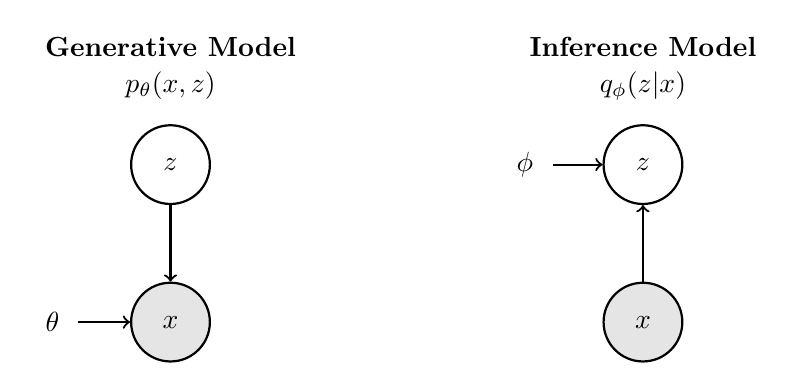
\begin{tikzpicture}[
        obs/.style={circle, draw, fill=gray!20, minimum size=1cm, thick},
        latent/.style={circle, draw, fill=white, minimum size=1cm, thick},
        param/.style={circle, draw=none, minimum size=0.5cm},
        arrow/.style={->, thick}
    ]
    % Generative Model
    \node[latent] (z_gen) at (0,0) {$z$};
    \node[obs] (x_gen) at (0,-2) {$x$};
    \node[param] (theta) at (-1.5,-2) {$\theta$};
    \draw[arrow] (z_gen) -- (x_gen);
    \draw[arrow] (theta) -- (x_gen);
    \node at (0, 1.5) {\textbf{Generative Model}};
    \node at (0, 1) {$p_\theta(x, z)$};
    
    % Inference Model
    \node[obs] (x_inf) at (6,-2) {$x$};
    \node[latent] (z_inf) at (6,0) {$z$};
    \node[param] (phi) at (4.5,0) {$\phi$};
    \draw[arrow] (x_inf) -- (z_inf);
    \draw[arrow] (phi) -- (z_inf);
    \node at (6, 1.5) {\textbf{Inference Model}};
    \node at (6, 1) {$q_\phi(z|x)$};
    \end{tikzpicture}
    \caption{Directed graphical models corresponding to the decoder (left) and the encoder (right).}
    \label{fig:graphical_model}
\end{figure}

The objective in AEVB is to maximize $\mathcal{L}(\theta, \phi; x)$ with respect to both $\theta$ and $\phi$. The $\mathbb{E}_{q_\phi(z|x)}[\log p_\theta(x|z)]$ term represents a reconstruction log-likelihood. The $D_{\text{KL}}(q_\phi(z|x) \parallel p_\theta(z))$ term acts as a complexity penalty, bounding the information rate required to encode $x$ into the latent representation $z$. 

\subsection{The Reparameterization Trick}
While optimizing $\theta$ via Monte Carlo sampling is trivial, optimizing the inference parameters $\phi$ is exceedingly difficult because the expectation is taken with respect to the distribution $q_\phi(z|x)$ itself. Using the standard REINFORCE algorithm yields gradients with prohibitively high variance. AEVB elegantly resolves this by deterministically reparameterizing the random variable $z$.

\begin{theorem}[The Reparameterization Trick]
\label{thm:reparam}
Let $z$ be a continuous random variable distributed according to $q_\phi(z|x)$. Suppose there exists a differentiable, deterministic transformation $g_\phi(x, \epsilon)$ and an independent base distribution $p(\epsilon)$ such that if $\epsilon \sim p(\epsilon)$, then $g_\phi(x, \epsilon) \sim q_\phi(z|x)$. The gradient of an expectation of a function $f(z)$ can be exactly expressed as:
\begin{equation}
    \nabla_\phi \mathbb{E}_{q_\phi(z|x)}[f(z)] = \mathbb{E}_{p(\epsilon)}[\nabla_\phi f(g_\phi(x, \epsilon))]
\end{equation}
\end{theorem}
\begin{proof}
By the Law of the Unconscious Statistician (LOTUS), we rewrite the expectation over $z$ as an expectation over the base noise variable $\epsilon$:
\begin{align}
    \nabla_\phi \mathbb{E}_{q_\phi(z|x)}[f(z)] &= \nabla_\phi \int q_\phi(z|x) f(z) dz \\
    &= \nabla_\phi \int p(\epsilon) f(g_\phi(x, \epsilon)) d\epsilon \\
    &= \int p(\epsilon) \nabla_\phi f(g_\phi(x, \epsilon)) d\epsilon \\
    &= \mathbb{E}_{p(\epsilon)}[\nabla_\phi f(g_\phi(x, \epsilon))]
\end{align}
Assuming standard regulatory conditions to exchange the gradient and the integral (such as dominated convergence), the gradient operator moves safely inside the expectation, allowing low-variance Monte Carlo estimation via deterministic backpropagation.
\end{proof}

\begin{figure}[htbp]
    \centering
    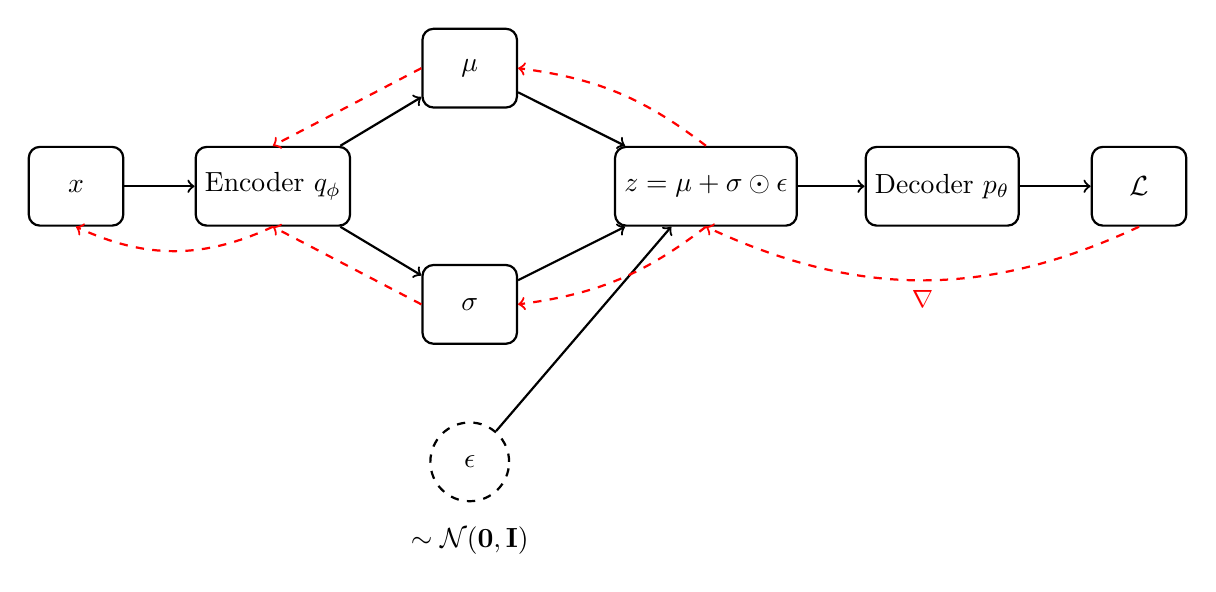
\begin{tikzpicture}[
        det/.style={rectangle, draw, rounded corners, minimum height=1cm, minimum width=1.2cm, thick},
        stoch/.style={circle, draw, dashed, minimum size=1cm, thick},
        arrow/.style={->, thick},
        grad/.style={->, thick, red, dashed}
    ]
    
    \node[det] (x) at (0,0) {$x$};
    \node[det] (enc) at (2.5,0) {Encoder $q_\phi$};
    \node[det] (mu) at (5,1.5) {$\mu$};
    \node[det] (sigma) at (5,-1.5) {$\sigma$};
    \node[stoch] (epsilon) at (5,-3.5) {$\epsilon$};
    \node[det] (z) at (8,0) {$z = \mu + \sigma \odot \epsilon$};
    \node[det] (dec) at (11,0) {Decoder $p_\theta$};
    \node[det] (loss) at (13.5,0) {$\mathcal{L}$};
    
    \draw[arrow] (x) -- (enc);
    \draw[arrow] (enc) -- (mu);
    \draw[arrow] (enc) -- (sigma);
    \draw[arrow] (mu) -- (z);
    \draw[arrow] (sigma) -- (z);
    \draw[arrow] (epsilon) -- (z);
    \draw[arrow] (z) -- (dec);
    \draw[arrow] (dec) -- (loss);
    
    % Backprop path
    \draw[grad] (loss.south) to[bend left=25] node[below] {\small $\nabla$} (z.south);
    \draw[grad] (z.north) to[bend right=15] (mu.east);
    \draw[grad] (z.south) to[bend left=15] (sigma.east);
    \draw[grad] (mu.west) -- (enc.north);
    \draw[grad] (sigma.west) -- (enc.south);
    \draw[grad] (enc.south) to[bend left=25] (x.south);
    
    \node[below] at (5,-4.2) {$\sim \mathcal{N}(\mathbf{0}, \mathbf{I})$};
    \end{tikzpicture}
    \caption{The Reparameterization Trick computational graph. Solid black arrows denote the forward evaluation pass. Dashed red arrows demonstrate the backpropagation gradients, entirely bypassing the stochastic noise node $\epsilon$.}
    \label{fig:reparam_trick}
\end{figure}

\subsection{Numerical Example: Gaussian Latent Space}
In modern implementations, the prior is overwhelmingly selected to be a standard isotropic multivariate Gaussian, $p_\theta(z) = \mathcal{N}(\mathbf{0}, \mathbf{I})$. The approximate posterior is mathematically enforced to be a multivariate Gaussian with a diagonal covariance matrix, $q_\phi(z|x) = \mathcal{N}(\mu, \text{diag}(\sigma^2))$, where both vectors are outputs of the neural network encoder.

The Kullback-Leibler divergence for a latent space of dimensionality $K$ under these conditions has a closed-form analytical solution:
\begin{equation}
    D_{\text{KL}}(\mathcal{N}(\mu, \text{diag}(\sigma^2)) \parallel \mathcal{N}(\mathbf{0}, \mathbf{I})) = \frac{1}{2} \sum_{k=1}^K \left( \sigma_k^2 + \mu_k^2 - 1 - \log(\sigma_k^2) \right)
\end{equation}

Let us step through a concrete numerical calculation. Suppose we are dealing with a $K=1$ dimensional latent space. Given a specific input $x_i$, our neural network encoder yields $\mu = 1.5$ and $\log(\sigma^2) = -0.5$.
This implies the variance is $\sigma^2 = \exp(-0.5) \approx 0.6065$, giving a standard deviation of $\sigma \approx 0.7788$.

We sample a standard normal noise variable $\epsilon \sim \mathcal{N}(0, 1)$. Suppose our random number generator provides $\epsilon = 0.8$. By Theorem \ref{thm:reparam}, the latent embedding is constructed as:
\begin{equation}
    z = \mu + \sigma \cdot \epsilon = 1.5 + 0.7788 \cdot 0.8 = 2.1230
\end{equation}
This scalar $z$ is then propagated to the decoder. Concurrently, the exact analytical KL divergence penalty acting on the parameters for this data point is computed as:
\begin{align}
    D_{\text{KL}} &= \frac{1}{2} \left( 0.6065 + (1.5)^2 - 1 - (-0.5) \right) \\
    &= \frac{1}{2} \left( 0.6065 + 2.25 - 1 + 0.5 \right) \\
    &= \frac{1}{2} \left( 2.3565 \right) = 1.17825
\end{align}
During the optimization phase, the KL gradient applies an elastic pull on $\mu$ towards $0$, and an elastic pull on $\log(\sigma^2)$ towards $0$ (yielding $\sigma^2 \to 1$). In competition, the reconstruction loss backpropagates through the sampled $z$, forcing $\mu$ and $\sigma$ to embed localized information unique to $x_i$, thereby achieving a delicate information-theoretic equilibrium.

\section{Horizon}
\begin{horizon}
The mathematical elegance of the AEVB framework assures us that we are deterministically maximizing a lower bound on the true data likelihood. Nonetheless, a substantial open problem remains regarding the ``amortization gap.'' It is conjectured that restricting inference to a feedforward network universally compromises the tightness of the ELBO compared to sample-specific iterative optimization strategies, such as Stochastic Gradient Langevin Dynamics. Future work might demonstrate that hybrid networks, combining feedforward predictions with iterative refinement steps in the latent space, can optimally close this gap without sacrificing inference speed.

Furthermore, a pervasive characteristic of the standard VAE is the blurriness of its generated samples. An intense debate remains open: is this blurriness an artifact of minimizing the expected $L_2$ norm (which rigidly assumes an isotropic Gaussian decoder likelihood), or does it arise intrinsically from the topological necessity of mapping a complex, disconnected data manifold into a dense, unimodal Gaussian prior? It is conjectured that integrating Normalizing Flows could fully close the ELBO gap, yet it remains an open question what such highly entangled prior flexibility would cost us concerning representation disentanglement.

Lastly, while AEVB seamlessly addresses continuous variables, porting these exact, unbiased, and low-variance gradient estimators to discrete categorical latent variables without resorting to biased soft-relaxations (like the Gumbel-Softmax) is a critical active frontier. We hypothesize that emerging discoveries in discrete variational bounds will eventually integrate AEVB into a sweeping, unified theory of discrete-continuous latent inference.
\end{horizon}

\section{Summary and Exercises}
\subsection{Summary}
In this chapter, we confronted the problem of intractable posterior inference within deep generative models using the Auto-Encoding Variational Bayes framework. By casting inference as a strict optimization problem, we bounded the log marginal likelihood with the Evidence Lower Bound (ELBO). To remedy the disastrous variance of gradients concerning the variational parameters, we proved the reparameterization trick, allowing gradients to deterministically flow backward through continuous random variables. 

\subsection{Exercises}
\begin{enumerate}
    \item \textbf{Analytical KL Divergence}: Prove the exact form of $D_{\text{KL}}(\mathcal{N}(\mu, \Sigma) \parallel \mathcal{N}(\mathbf{0}, \mathbf{I}))$ for a multivariate Gaussian with an arbitrary dense covariance matrix $\Sigma$. 
    \item \textbf{Variance Reduction Verification}: Consider a simple optimization of the expectation of $f(z) = z^2$. Compare the theoretical variance of the gradient estimator obtained via the standard REINFORCE (score function) algorithm to the variance of the gradient obtained via the reparameterization trick when $q(z|\phi) = \mathcal{N}(\phi, 1)$. Prove mathematically that the reparameterization trick possesses strictly lower variance.
    \item \textbf{The ELBO Gap}: Analytically prove that the discrepancy between the true log-marginal likelihood $\log p_\theta(x)$ and the ELBO $\mathcal{L}(\theta, \phi; x)$ is precisely equivalent to the Kullback-Leibler divergence between the approximate posterior and the true posterior. 
\end{enumerate}

% TODO-CITE: Ensure all named results are cited.

\chapter{Disentanglement and $\beta$-VAEs}
\label{ch:beta_vae}

\section{The Quest for Factored Representations}

A central aspiration of unsupervised learning is to discover representations that carve nature at its joints. In the physical world, sensory observations are generated by the complex interaction of independent generative factors. When we look at a scene, the pixel intensities on our retina are the entangled result of lighting conditions, object geometry, color, and viewpoint. To human perception, however, these factors are distinct and independently manipulable. We can imagine the same object painted a different color, or viewed from a different angle, without altering its fundamental identity.

In the parlance of deep learning, representations that successfully separate these independent sources of variation are said to be \textit{disentangled}. A perfectly disentangled latent space aligns its coordinate axes with the true, underlying generative factors of the data. If the representation is an $M$-dimensional vector $z$, a change in a single dimension $z_i$ should correspond to a change in exactly one ground-truth factor (e.g., the azimuth angle of a face), while leaving all other factors invariant.

The Auto-Encoding Variational Bayes framework, developed in Chapters 12 and 13, provides a powerful generative mechanism but does not inherently guarantee disentanglement. The standard Variational Autoencoder (VAE) optimizes the Evidence Lower Bound (ELBO), which balances the reconstruction fidelity of the data against the divergence of the approximate posterior $q_\phi(z|x)$ from a prior $p(z)$. While this forces the latent space to be continuous and well-behaved, the standard VAE often learns entangled representations where a single semantic concept is distributed across multiple latent dimensions.

The $\beta$-VAE, introduced by Higgins et al., elegantly tackles this limitation through a minimal modification to the standard ELBO. By introducing an adjustable hyperparameter $\beta > 1$, the $\beta$-VAE places a heavier penalty on the Kullback-Leibler (KL) divergence between the approximate posterior and the prior. 

Why should penalizing the KL divergence induce disentanglement? The standard prior $p(z)$ is typically chosen to be an isotropic multivariate Gaussian, $p(z) = \mathcal{N}(0, I)$. A crucial property of this prior is that its components are statistically independent: $p(z) = \prod_{j} p(z_j)$. By forcing the aggregate posterior to closely match this factorized prior, the $\beta$-VAE objective applies immense pressure on the latent dimensions to become independent of one another. Assuming the true data-generating process relies on independent factors, matching the independent structure of the prior encourages the model to align its latent dimensions with these true factors, spontaneously yielding disentanglement.

This intuitive mechanism, however, masks a deeper information-theoretic phenomenon. When we heavily penalize the KL divergence to the prior, we are simultaneously restricting the information capacity of the latent bottleneck. The network is forced to discard the complex, high-order correlations that entangle variables, retaining only the most statistically independent and prominent features. In this chapter, we will strip away the heuristic explanations and rigorously analyze the $\beta$-VAE objective. We will decompose the KL divergence penalty to reveal the exact terms responsible for disentanglement, mathematically connect it to the Information Bottleneck principle, and demonstrate the unavoidable theoretical limits of purely unsupervised disentangled representation learning.

\section{The Information-Theoretic Foundations of $\beta$-VAE}

We begin by formally defining the $\beta$-VAE objective. Let $x \in \mathcal{X}$ be the observed data and $z$ be the continuous latent variables. The encoder (inference model) is parameterized by $\phi$ as $q_\phi(z|x)$, and the decoder (generative model) is parameterized by $\theta$ as $p_\theta(x|z)$.

\begin{definition}[$\beta$-VAE Objective]
For a given data point $x \sim P_{\text{data}}$, the $\beta$-VAE minimizes the following negative log-likelihood bound:
\begin{equation}
    \mathcal{L}_\beta(\theta, \phi; x) = -\mathbb{E}_{q_\phi(z|x)}[\log p_\theta(x|z)] + \beta D_{\text{KL}}(q_\phi(z|x) \parallel p(z))
\end{equation}
where $\beta \geq 0$ is the regularization coefficient. The standard VAE is recovered when $\beta = 1$.
\end{definition}

This modification can be derived rigorously from a constrained optimization perspective using the Information Bottleneck (IB) principle (Chapter 8). Suppose we wish to maximize the reconstruction likelihood, but we are subject to a strict upper bound on the channel capacity between the input $X$ and the latent space $Z$.

\begin{theorem}[Mutual Information Bound on the Latent Space]
\label{thm:mi_bound}
The expected KL divergence between the approximate posterior $q_\phi(z|x)$ and the prior $p(z)$ is a strict upper bound on the mutual information $I(X; Z)$ between the data and the latent representation under the empirical data distribution $p_{\text{data}}(x)$. Specifically,
\begin{equation}
    \mathbb{E}_{p_{\text{data}}(x)} \left[ D_{\text{KL}}(q_\phi(z|x) \parallel p(z)) \right] = I(X; Z) + D_{\text{KL}}(q(z) \parallel p(z))
\end{equation}
where $q(z) = \mathbb{E}_{p_{\text{data}}(x)}[q_\phi(z|x)]$ is the aggregate posterior.
\end{theorem}

\begin{proof}
Let us write the expected KL divergence explicitly:
\begin{align}
    \mathbb{E}_{p_{\text{data}}(x)} \left[ D_{\text{KL}}(q_\phi(z|x) \parallel p(z)) \right] &= \int p_{\text{data}}(x) \int q_\phi(z|x) \log \frac{q_\phi(z|x)}{p(z)} dz dx \\
    &= \iint p_{\text{data}}(x) q_\phi(z|x) \left( \log \frac{q_\phi(z|x)}{q(z)} + \log \frac{q(z)}{p(z)} \right) dz dx \\
    &= \iint p_{\text{data}}(x) q_\phi(z|x) \log \frac{q_\phi(z|x)}{q(z)} dz dx + \int \left( \int p_{\text{data}}(x) q_\phi(z|x) dx \right) \log \frac{q(z)}{p(z)} dz \\
    &= I(X; Z) + \int q(z) \log \frac{q(z)}{p(z)} dz \\
    &= I(X; Z) + D_{\text{KL}}(q(z) \parallel p(z))
\end{align}
Since the Kullback-Leibler divergence is non-negative ($D_{\text{KL}}(q(z) \parallel p(z)) \geq 0$), it follows that $\mathbb{E}_{p_{\text{data}}(x)} \left[ D_{\text{KL}}(q_\phi(z|x) \parallel p(z)) \right] \geq I(X; Z)$.
\end{proof}

\begin{figure}[htbp]
    \centering
    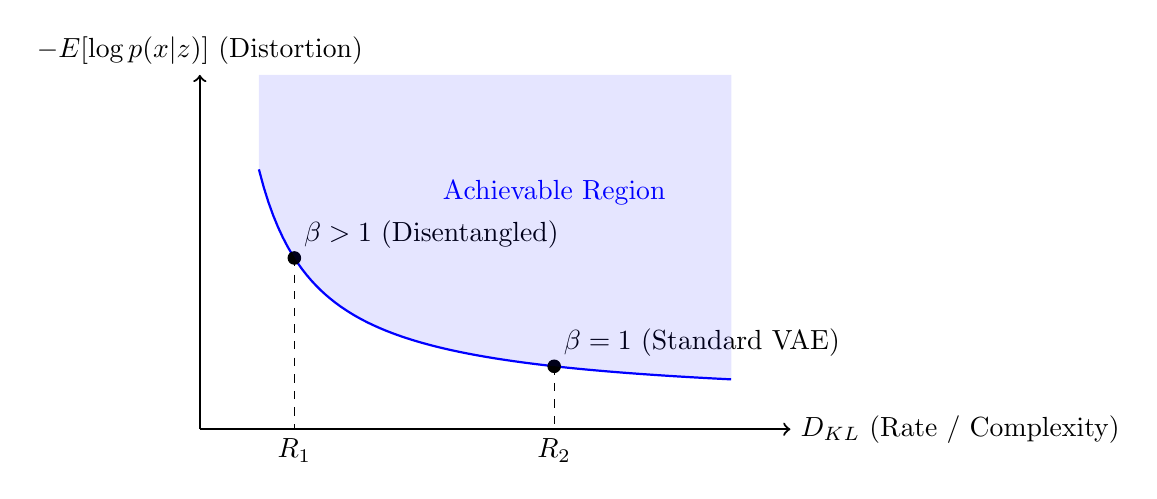
\begin{tikzpicture}[scale=1.5]
        % Axes
        \draw[->, thick] (0,0) -- (5,0) node[right] {$D_{\text{KL}}$ (Rate / Complexity)};
        \draw[->, thick] (0,0) -- (0,3) node[above] {$-\mathbb{E}[\log p(x|z)]$ (Distortion)};
        
        % Curve
        \draw[thick, blue, domain=0.5:4.5, samples=100] plot (\x, {1/\x + 0.2});
        
        % Points
        \filldraw[black] (0.8, 1.45) circle (1.5pt) node[anchor=south west] {$\beta > 1$ (Disentangled)};
        \filldraw[black] (3.0, 0.533) circle (1.5pt) node[anchor=south west] {$\beta=1$ (Standard VAE)};
        
        % Feasible region
        \fill[blue, opacity=0.1] (0.5, 3) -- plot[domain=0.5:4.5] (\x, {1/\x + 0.2}) -- (4.5, 3) -- cycle;
        \node[blue] at (3, 2) {Achievable Region};
        
        % Labels for Rate
        \draw[dashed] (0.8, 1.45) -- (0.8, 0) node[below] {$R_1$};
        \draw[dashed] (3.0, 0.533) -- (3.0, 0) node[below] {$R_2$};
    \end{tikzpicture}
    \caption{The Information Bottleneck interpretation of the $\beta$-VAE. By increasing $\beta$, we force the model to operate at a lower rate ($R_1 < R_2$), increasing the bottleneck pressure. This reduction in capacity forces the network to abandon entangled representations in favor of the most statistically independent, fundamental factors.}
    \label{fig:beta_vae_tradeoff}
\end{figure}

This theorem provides profound insight into the $\beta$-VAE. The objective is mathematically equivalent to minimizing the distortion (reconstruction error) subject to a Lagrangian penalty on the information channel capacity between data and latents. When $\beta > 1$, we aggressively throttle this capacity.

\section{Decomposition of the Evidence Lower Bound}

To understand precisely how disentanglement emerges, we must analyze the structure of the aggregate posterior $q(z)$. Assuming the latent space is $D$-dimensional, $z = [z_1, z_2, \dots, z_D]^\top$, the factorized prior is $p(z) = \prod_{j=1}^D p(z_j)$.

\begin{theorem}[KL Decomposition]
\label{thm:kl_decomp}
The expected KL divergence penalty in the $\beta$-VAE objective decomposes into three distinct information-theoretic terms:
\begin{equation}
    \mathbb{E}_{p_{\text{data}}(x)} \left[ D_{\text{KL}}(q_\phi(z|x) \parallel p(z)) \right] = I(X; Z) + TC(Z) + \sum_{j=1}^D D_{\text{KL}}(q(z_j) \parallel p(z_j))
\end{equation}
where $q(z_j)$ is the marginal distribution of the $j$-th latent dimension, and $TC(Z)$ is the Total Correlation of the latent variables.
\end{theorem}

\begin{proof}
By Theorem \ref{thm:mi_bound}, we know the expected KL is equal to $I(X;Z) + D_{\text{KL}}(q(z) \parallel p(z))$. We now decompose the second term, the marginal KL divergence to the prior:
\begin{align}
    D_{\text{KL}}(q(z) \parallel p(z)) &= \int q(z) \log \frac{q(z)}{p(z)} dz \\
    &= \int q(z) \log \frac{q(z)}{\prod_{j=1}^D q(z_j)} \frac{\prod_{j=1}^D q(z_j)}{\prod_{j=1}^D p(z_j)} dz \\
    &= \int q(z) \log \frac{q(z)}{\prod_{j=1}^D q(z_j)} dz + \int q(z) \sum_{j=1}^D \log \frac{q(z_j)}{p(z_j)} dz \\
    &= D_{\text{KL}}\left( q(z) \parallel \prod_{j=1}^D q(z_j) \right) + \sum_{j=1}^D \int q(z_j) \log \frac{q(z_j)}{p(z_j)} dz_j \\
    &= TC(Z) + \sum_{j=1}^D D_{\text{KL}}(q(z_j) \parallel p(z_j))
\end{align}
Substituting this back into the identity from Theorem \ref{thm:mi_bound} completes the proof.
\end{proof}

\begin{figure}[htbp]
    \centering
    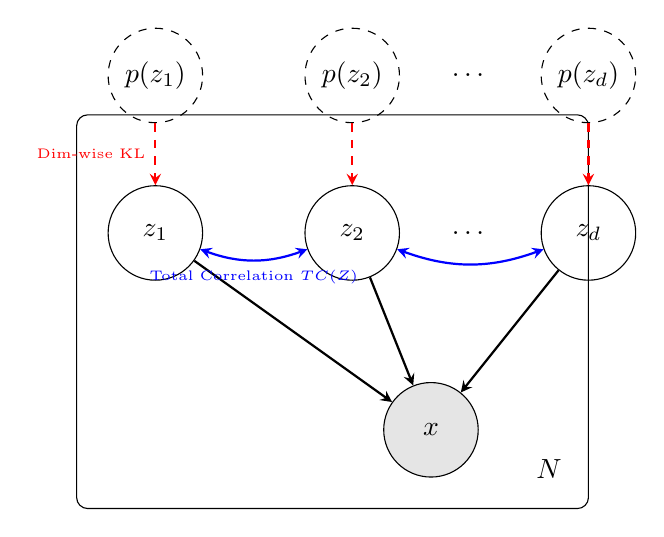
\begin{tikzpicture}[
        node distance=2.5cm,
        obs/.style={circle, draw, fill=gray!20, minimum size=1.2cm},
        lat/.style={circle, draw, minimum size=1.2cm},
        edge/.style={->, >=stealth, thick}
    ]
        % Prior nodes
        \node[lat, dashed] (pz1) {$p(z_1)$};
        \node[lat, dashed, right of=pz1] (pz2) {$p(z_2)$};
        \node[right of=pz2, node distance=1.5cm] (dots1) {\dots};
        \node[lat, dashed, right of=dots1, node distance=1.5cm] (pzd) {$p(z_d)$};
        
        % Latent nodes
        \node[lat, below of=pz1, node distance=2cm] (z1) {$z_1$};
        \node[lat, below of=pz2, node distance=2cm] (z2) {$z_2$};
        \node[below of=dots1, node distance=2cm] (dots2) {\dots};
        \node[lat, below of=pzd, node distance=2cm] (zd) {$z_d$};
        
        % Observation node
        \node[obs, below of=z2, node distance=2.5cm, xshift=1cm] (x) {$x$};
        
        % Plate
        \draw[rounded corners] (-1, -5.5) rectangle (5.5, -0.5);
        \node at (5, -5) {$N$};
        
        % Edges
        \draw[edge] (z1) -- (x);
        \draw[edge] (z2) -- (x);
        \draw[edge] (zd) -- (x);
        
        \draw[edge, dashed, red] (pz1) -- (z1) node[midway, left] {\tiny Dim-wise KL};
        \draw[edge, dashed, red] (pz2) -- (z2);
        \draw[edge, dashed, red] (pzd) -- (zd);
        
        \draw[<->, >=stealth, thick, blue] (z1) to[bend right=20] node[midway, below] {\tiny Total Correlation $TC(Z)$} (z2);
        \draw[<->, >=stealth, thick, blue] (z2) to[bend right=20] (zd);
        
    \end{tikzpicture}
    \caption{The decomposition of the $\beta$-VAE penalty. The objective implicitly penalizes the dimension-wise KL divergence (red, forcing marginals to match the prior), the Total Correlation (blue, forcing latent variables to be independent), and the mutual information $I(X;Z)$ (the dependence between $x$ and $z$).}
    \label{fig:beta_vae_decomp}
\end{figure}

Let us analyze the three resultant penalty terms:
\begin{enumerate}
    \item \textbf{Index-Code Mutual Information, $I(X; Z)$:} Penalizing this term explicitly restricts the channel capacity, acting as an Information Bottleneck. It forces the representation to be highly compressed.
    \item \textbf{Total Correlation, $TC(Z)$:} This is a generalization of mutual information to multiple variables. It equals zero if and only if the latent variables $z_j$ are perfectly independent under the aggregate posterior $q(z)$. \textit{This is the core mechanism that drives disentanglement.} By multiplying the expected KL by $\beta > 1$, we place an immense penalty on $TC(Z)$, forcing the network to discover statistically independent latent representations.
    \item \textbf{Dimension-wise KL, $\sum_j D_{\text{KL}}(q(z_j) \parallel p(z_j))$:} This acts as a regularizer to ensure the marginal distribution of each latent dimension does not collapse or diverge infinitely far from the standard normal prior.
\end{enumerate}

\section{Numerical Example: Phase Transitions in Linear $\beta$-VAE}

To concretize this, consider a linear $\beta$-VAE. Suppose the true data is generated as $x \sim \mathcal{N}(0, \Sigma_x)$ where $x \in \mathbb{R}^N$. The generative model is $p_\theta(x|z) = \mathcal{N}(Wz, \sigma^2 I)$ and the prior is $p(z) = \mathcal{N}(0, I)$ for $z \in \mathbb{R}^K$. The approximate posterior is $q_\phi(z|x) = \mathcal{N}(Vx, \text{diag}(\sigma_{z}^2))$.

If we optimize the $\beta$-VAE objective analytically, we observe a phenomenon known as \textit{posterior collapse}, heavily dependent on the value of $\beta$. Let $\lambda_k$ be the $k$-th eigenvalue of the data covariance matrix $\Sigma_x$, ordered such that $\lambda_1 \geq \lambda_2 \geq \dots \geq \lambda_K$.

For a given dimension $k$ in the latent space, if $\beta$ is sufficiently large, specifically if:
\begin{equation}
    \beta > \frac{\lambda_k}{\sigma^2}
\end{equation}
then the optimal solution dictates that the $k$-th latent dimension completely collapses to the prior: $V_k = 0$ (where $V_k$ is the $k$-th row of $V$) and $\sigma_{z,k}^2 = 1$. The network entirely severs the mutual information between $x$ and $z_k$. 

As $\beta$ decreases, dimensions "activate" sequentially, starting with the one aligned with the largest principal component $\lambda_1$. This demonstrates how $\beta$ acts as a strict information throttle: it prunes away latent dimensions that capture low-variance (and thus, less informative) factors of variation, forcing the model to allocate its limited channel capacity exclusively to the most dominant, independent factors of the data.

\begin{horizon}
It is mathematically proved that purely unsupervised learning of disentangled representations is fundamentally impossible without structural inductive biases. Locatello et al. (2019) elegantly demonstrated that for any perfectly disentangled generative model, there exists an infinite family of alternative, highly entangled models that produce the exact same marginal data distribution $p(x)$. Because the ELBO depends on the data only through the marginal likelihood, the $\beta$-VAE—and any purely unsupervised method—cannot theoretically distinguish between the true disentangled model and an entangled equivalent.

It is conjectured that the empirical success of $\beta$-VAEs on specific datasets is driven not purely by the objective function, but by the implicit regularization provided by neural network architectures (such as the locality of convolutions) and the specific hyperparameters chosen. Future work might show that weak supervision, temporal continuity in sequential data, or carefully engineered non-Gaussian priors are theoretically necessary conditions to guarantee the identifiability of true latent factors. An open question remains whether we can design foundational models that inherently leverage these multi-view or temporal symmetries to bypass these impossibility theorems, shifting the field from heuristic regularization to guaranteed disentanglement.
\end{horizon}

\section{Summary}
\begin{itemize}
    \item Disentanglement seeks representations where single latent units correspond to single, independent factors of variation in the generative process of the data.
    \item The $\beta$-VAE objective introduces a hyperparameter $\beta > 1$ to heavily penalize the KL divergence between the approximate posterior and the prior.
    \item The expected KL divergence mathematically acts as a strict upper bound on the mutual information $I(X;Z)$, linking the $\beta$-VAE directly to the Information Bottleneck principle.
    \item The objective decomposes into the index-code mutual information, the Total Correlation (TC), and the dimension-wise KL divergence. Penalizing the Total Correlation is the primary driver of statistical independence and disentanglement.
    \item In linear models, increasing $\beta$ sequentially forces latent dimensions to collapse to the prior, naturally pruning less significant factors of variation.
\end{itemize}

\section*{Exercises}
\begin{enumerate}
    \item \textbf{Deriving the KL Bound on Mutual Information:} Prove step-by-step that $\mathbb{E}_{p_{\text{data}}(x)} [D_{\text{KL}}(q_\phi(z|x) \parallel p(z))] = I(X;Z) + D_{\text{KL}}(q(z) \parallel p(z))$, where $q(z) = \mathbb{E}_{p_{\text{data}}(x)}[q_\phi(z|x)]$. Using this result, prove that the $\beta$-VAE penalty strictly upper bounds the mutual information $I(X;Z)$.
    \item \textbf{Phase Transitions in the Linear $\beta$-VAE:} Consider a linear Gaussian $\beta$-VAE where $x \in \mathbb{R}$ and $z \in \mathbb{R}$. Given $p_{\text{data}}(x) = \mathcal{N}(0, \sigma_x^2)$, $p_\theta(x|z) = \mathcal{N}(w z, 1)$, and $q_\phi(z|x) = \mathcal{N}(v x, s^2)$, write out the expected ELBO. Derive the optimal values $v^*$ and $s^*$ as a function of $\beta, w$, and $\sigma_x^2$, and mathematically show the condition under which the latent dimension completely collapses ($s^* = 1, v^* = 0$).
    \item \textbf{Total Correlation of a Bivariate Gaussian:} Suppose the aggregate posterior $q(z_1, z_2)$ is a bivariate Gaussian with zero mean, unit variances, and correlation coefficient $\rho$. Calculate the Total Correlation $TC(Z) = D_{\text{KL}}(q(z_1, z_2) \parallel q(z_1)q(z_2))$ as an explicit function of $\rho$. Discuss how minimizing this term affects the covariance structure of the latent space.
\end{enumerate}

% TODO-CITE: Ensure all named results are cited.

\chapter{Rate-Distortion Theory in Latent Spaces}
\label{ch:rate_distortion}

\section{The Geometry of Compression: An Introduction}

In deep learning, the representations learned by autoencoders are frequently interpreted through the lens of feature extraction, manifold learning, and dimensionality reduction. While these perspectives are powerful, they often lack a strict, quantifiable measure of representation optimality. A more fundamental perspective arises from information theory, specifically \emph{rate-distortion theory}. Formulated by Claude Shannon in 1959, rate-distortion theory establishes the absolute theoretical limits of lossy data compression. It addresses a profound question: what is the minimum number of bits per symbol (the \emph{rate}) required to represent a source signal such that it can be reconstructed with an expected error no greater than a specified threshold (the \emph{distortion})?

When applied to latent variable models such as the Variational Autoencoder (VAE), rate-distortion theory provides a rigorous mathematical framework for understanding the core trade-off governing deep generative models. It elucidates the tension between the complexity of the latent representation $z$ and the fidelity of the reconstructed input $x$. In this chapter, we explore how modern neural networks implicitly and explicitly navigate these theoretical bounds.

In an ideal, noiseless scenario, we might wish to represent our dataset $\mathcal{D} = \{x_1, \dots, x_N\} \sim P_{\text{data}}$ with zero error. However, the continuous nature of high-dimensional data—such as natural images, audio waveforms, or dense textual embeddings—implies that exact representation requires infinite precision, and thus, infinite bits. Consequently, any continuous latent space compression is inherently lossy. A neural network is forced to decide which features of the input space $\mathcal{X}$ are essential and which can be discarded as noise. This decision process is not arbitrary; it is governed by the structural constraints placed on the bottleneck.

The inference model (or encoder) $q_\phi(z|x)$ dictates the mapping from the data manifold into the latent space. The stochasticity inherent in $q_\phi(z|x)$ can be viewed mathematically as a noisy communication channel. By injecting variance into the encodings, the model limits the channel capacity, thereby constraining the rate of information flow. This is distinct from deterministic autoencoders, which must rely on explicitly restricting the dimensionality of the bottleneck. In stochastic models, even a high-dimensional latent space can have a low effective rate if the variance of the injected noise is sufficiently large relative to the signal.

The generative model (or decoder) $p_\theta(x|z)$ subsequently attempts to invert this mapping, transforming the compressed latent code back into the original data space. The quality of this inversion is measured by a distortion function, commonly the mean squared error for continuous variables or cross-entropy for categorical data. The optimization landscape is therefore a tug-of-war: the encoder is pressured to transmit more information to lower the distortion, while the prior exerts a regularizing force that penalizes high transmission rates.

By interpreting the objective functions of deep generative models through this theoretical lens, we uncover a direct correspondence between empirical optimization and the foundational limits of information theory. As we will demonstrate mathematically, the regularization terms in models like the $\beta$-VAE restrict the transmission rate, while the reconstruction terms penalize distortion. This perspective unifies disparate empirical observations and provides a principled mechanism for controlling the trade-off between latent disentanglement, aggressive compression, and generation quality.

\section{Formalizing the Rate-Distortion Trade-off}

To formalize these concepts, we consider an input space $\mathcal{X}$ populated by a random variable $X \sim P_{\text{data}}(x)$, and a latent space defined by a random variable $Z$. We further define a non-negative distortion measure $d: \mathcal{X} \times \mathcal{X} \to \mathbb{R}_{\ge 0}$, where $d(x, \hat{x})$ quantifies the cost of representing the original data point $x$ by its reconstruction $\hat{x}$.

\begin{definition}[Rate-Distortion Function]
Given a source distribution $P_{\text{data}}(x)$ and a distortion measure $d(x, \hat{x})$, the rate-distortion function $R(D)$ is defined as the minimum mutual information between $X$ and its reconstruction $\hat{X}$ such that the expected distortion is bounded by a threshold $D$:
\begin{equation}
    R(D) = \min_{p(\hat{x}|x) : \mathbb{E}[d(X, \hat{X})] \le D} I(X; \hat{X})
\end{equation}
\end{definition}

In the context of latent variable models parameterized by neural networks, the information bottleneck lies between $X$ and $Z$. The representation $Z$ is then decoded into the reconstruction $\hat{X}$. The sequence of transformations $X \to Z \to \hat{X}$ forms a Markov chain.

\begin{lemma}[Data Processing Inequality for Autoencoders]
For the Markov chain $X \to Z \to \hat{X}$ defined by an encoder $q_\phi(z|x)$ and a decoder $p_\theta(x|z)$, the mutual information satisfies:
\begin{equation}
    I(X; \hat{X}) \le I(X; Z)
\end{equation}
\end{lemma}
\begin{proof}
By the chain rule for mutual information, we can expand the joint mutual information $I(X; Z, \hat{X})$ in two equivalent ways:
\begin{align*}
    I(X; Z, \hat{X}) &= I(X; Z) + I(X; \hat{X} | Z) \\
    &= I(X; \hat{X}) + I(X; Z | \hat{X})
\end{align*}
Because $X \to Z \to \hat{X}$ is a Markov chain, $X$ and $\hat{X}$ are conditionally independent given $Z$. Therefore, $I(X; \hat{X} | Z) = 0$. This simplifies our equation to:
\begin{equation*}
    I(X; Z) = I(X; \hat{X}) + I(X; Z | \hat{X})
\end{equation*}
Since mutual information is fundamentally non-negative, $I(X; Z | \hat{X}) \ge 0$, and thus $I(X; \hat{X}) \le I(X; Z)$.
\end{proof}

This lemma has a profound implication: minimizing the rate of the latent bottleneck $I(X;Z)$ effectively places an upper bound on the true rate $I(X; \hat{X})$ transmitted through the entire autoencoder pipeline. 

\begin{figure}[htbp]
\centering
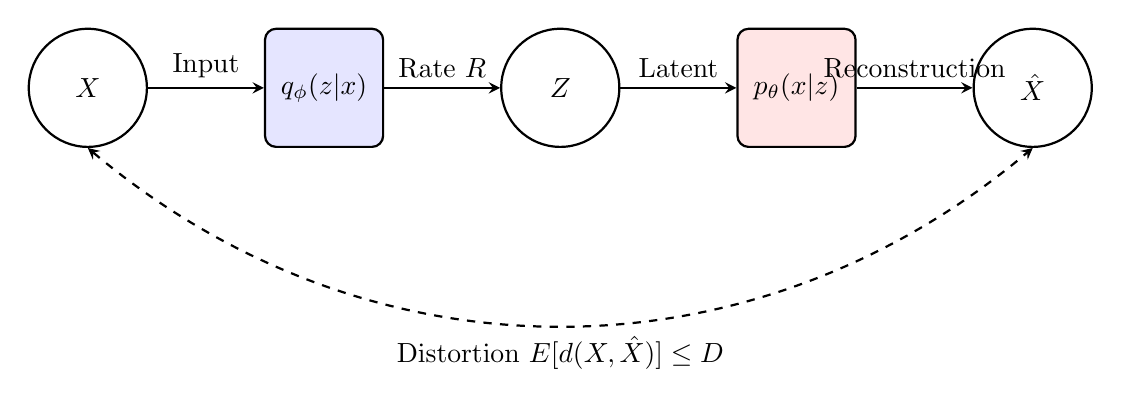
\begin{tikzpicture}[node distance=3cm, >=stealth, thick]
    % Nodes
    \node[draw, circle, minimum size=1.5cm] (X) at (0, 0) {$X$};
    \node[draw, rectangle, rounded corners, minimum size=1.5cm, fill=blue!10] (Enc) at (3, 0) {$q_\phi(z|x)$};
    \node[draw, circle, minimum size=1.5cm] (Z) at (6, 0) {$Z$};
    \node[draw, rectangle, rounded corners, minimum size=1.5cm, fill=red!10] (Dec) at (9, 0) {$p_\theta(x|z)$};
    \node[draw, circle, minimum size=1.5cm] (Xhat) at (12, 0) {$\hat{X}$};
    
    % Edges
    \draw[->] (X) -- (Enc) node[midway, above] {Input};
    \draw[->] (Enc) -- (Z) node[midway, above] {Rate $R$};
    \draw[->] (Z) -- (Dec) node[midway, above] {Latent};
    \draw[->] (Dec) -- (Xhat) node[midway, above] {Reconstruction};
    
    % Distortion annotation
    \draw[<->, dashed, bend right=40] (X.south) to node[below] {Distortion $\mathbb{E}[d(X, \hat{X})] \le D$} (Xhat.south);
\end{tikzpicture}
\caption{The Markov chain $X \to Z \to \hat{X}$ induced by an autoencoder. Information flows through the stochastic encoder, establishing a rate limit, while the decoder attempts to minimize the expected distortion.}
\label{fig:rd_markov}
\end{figure}

\begin{theorem}[VAE Objective as a Rate-Distortion Bound]
Let $q_\phi(z|x)$ be an encoder and $p_\theta(x|z)$ be a decoder. Define the distortion measure as the expected negative log-likelihood, $d(x, z) = -\log p_\theta(x|z)$. The optimization objective of the $\beta$-VAE, denoted $\mathcal{L}(\theta, \phi; \beta)$, minimizes an upper bound on the rate for a given distortion.
\end{theorem}
\begin{proof}
Consider the mutual information between the data $X$ and the latent variable $Z$ under the joint distribution $p(x, z) = P_{\text{data}}(x)q_\phi(z|x)$. We can expand $I(X;Z)$ as follows:
\begin{align}
    I(X;Z) &= \iint P_{\text{data}}(x) q_\phi(z|x) \log \frac{q_\phi(z|x)}{q_\phi(z)} \, dz \, dx \nonumber \\
    &= \mathbb{E}_{P_{\text{data}}(x)}\left[ D_{\text{KL}}(q_\phi(z|x) \parallel q_\phi(z)) \right]
\end{align}
where $q_\phi(z) = \mathbb{E}_{P_{\text{data}}(x)}[q_\phi(z|x)]$ is the aggregated posterior distribution. 

In a standard Variational Autoencoder, we specify a simple prior $p(z)$ (usually an isotropic normal distribution). We can rewrite the logarithm by introducing $p(z)$:
\begin{align}
    \mathbb{E}_{P_{\text{data}}(x)}\left[ D_{\text{KL}}(q_\phi(z|x) \parallel p(z)) \right] &= \iint P_{\text{data}}(x) q_\phi(z|x) \log \frac{q_\phi(z|x)}{p(z)} \, dz \, dx \nonumber \\
    &= \iint P_{\text{data}}(x) q_\phi(z|x) \left( \log \frac{q_\phi(z|x)}{q_\phi(z)} + \log \frac{q_\phi(z)}{p(z)} \right) \, dz \, dx \nonumber \\
    &= I(X;Z) + D_{\text{KL}}(q_\phi(z) \parallel p(z))
\end{align}
Because the Kullback-Leibler divergence is strictly non-negative ($D_{\text{KL}}(q_\phi(z) \parallel p(z)) \ge 0$), it immediately follows that:
\begin{equation}
    I(X;Z) \le \mathbb{E}_{P_{\text{data}}(x)}\left[ D_{\text{KL}}(q_\phi(z|x) \parallel p(z)) \right]
\end{equation}
This establishes an upper bound on the rate, which we denote as $R_{UB}$. 

The expected distortion under our negative log-likelihood measure is:
\begin{equation}
    D_{\text{expected}} = \mathbb{E}_{P_{\text{data}}(x)}\left[ \mathbb{E}_{q_\phi(z|x)}[-\log p_\theta(x|z)] \right]
\end{equation}
The $\beta$-VAE loss function is precisely the unconstrained Lagrangian formulation of the rate-distortion optimization problem:
\begin{equation}
    \mathcal{L}(\theta, \phi; \beta) = D_{\text{expected}} + \beta R_{UB}
\end{equation}
Thus, minimizing $\mathcal{L}(\theta, \phi; \beta)$ implicitly minimizes an upper bound on the transmission rate while explicitly minimizing the expected distortion, mapped out over the Pareto frontier by varying the Lagrange multiplier $\beta$.
\end{proof}

\begin{figure}[htbp]
\centering
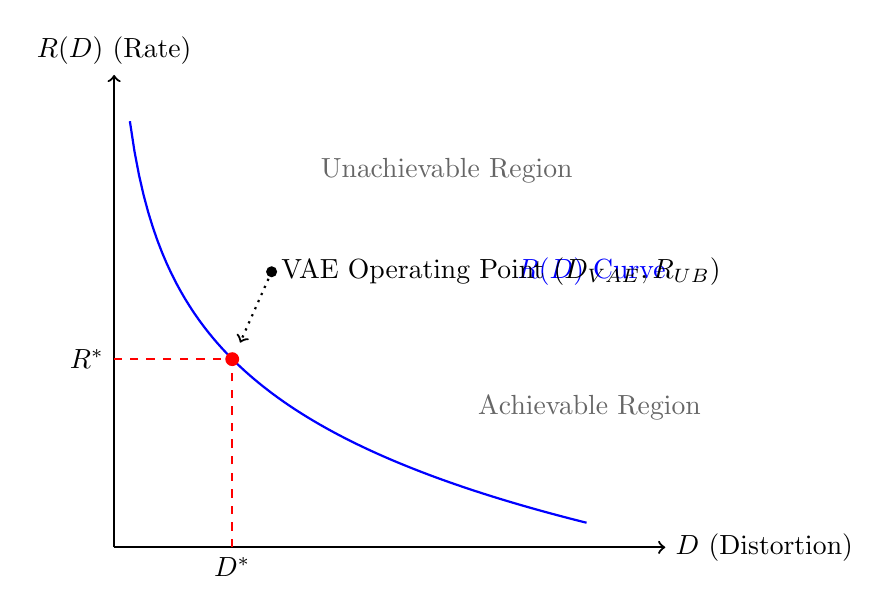
\begin{tikzpicture}
    % Axes
    \draw[->, thick] (0, 0) -- (7, 0) node[right] {$D$ (Distortion)};
    \draw[->, thick] (0, 0) -- (0, 6) node[above] {$R(D)$ (Rate)};
    
    % Curve
    \draw[thick, blue, domain=0.2:6, samples=100] plot (\x, {max(0, -1.5*ln(\x) + 3)});
    
    % Annotations
    \node at (2.5, 4.5) [anchor=south west, text=black!60] {Unachievable Region};
    \node at (4.5, 1.5) [anchor=south west, text=black!60] {Achievable Region};
    \node at (5, 3.5) [anchor=west, text=blue] {$R(D)$ Curve};
    
    % Dashed lines for a specific point
    \draw[dashed, thick, red] (1.5, 0) node[below, text=black] {$D^*$} -- (1.5, 2.39) -- (0, 2.39) node[left, text=black] {$R^*$};
    \fill[red] (1.5, 2.39) circle (2.5pt);
    
    % Example of VAE Bound
    \fill[black] (2.0, 3.5) circle (2pt) node[right] {VAE Operating Point ($D_{\text{VAE}}, R_{UB}$)};
    \draw[->, dotted, thick] (2.0, 3.5) -- (1.6, 2.6);
\end{tikzpicture}
\caption{The rate-distortion function $R(D)$ forms a monotonically decreasing, convex curve that separates achievable compressions from impossible ones. A real-world VAE operates at a point $(D_{\text{VAE}}, R_{UB})$ that is strictly sub-optimal, lying within the achievable region above the theoretical curve.}
\label{fig:rd_curve2}
\end{figure}

\subsection*{Numerical Example: The Gaussian Source}
Consider a scalar Gaussian source $X \sim \mathcal{N}(0, \sigma_x^2)$ and a squared-error distortion measure $d(x, \hat{x}) = (x - \hat{x})^2$. It is a well-known analytical result in information theory that the rate-distortion function for this continuous source is given by:
\begin{equation}
    R(D) = 
    \begin{cases} 
      \frac{1}{2} \log_2 \left( \frac{\sigma_x^2}{D} \right) & \text{if } 0 < D \le \sigma_x^2 \\
      0 & \text{if } D > \sigma_x^2
    \end{cases}
\end{equation}
Let the source variance be $\sigma_x^2 = 1$. Suppose we mandate a reconstruction with a maximum expected mean squared error of $D = 0.25$. Substituting this requirement into our formula yields the theoretical minimum transmission rate:
\begin{equation}
    R(0.25) = \frac{1}{2} \log_2\left(\frac{1}{0.25}\right) = \frac{1}{2} \log_2(4) = 1 \text{ bit}.
\end{equation}
This mathematically guarantees that any optimal encoder mapping $X$ to a continuous latent space $Z$ must transmit exactly 1 bit of mutual information per symbol to allow the decoder to achieve an MSE of 0.25. 

If a $\beta$-VAE is trained on this data, the KL divergence penalty bounds the mutual information. If this penalty term approaches 1 bit from above, the network is nearing optimal channel capacity. Conversely, if the KL term is regularized to drop below 1 bit, it is theoretically impossible for the expected reconstruction MSE to remain at or below 0.25. The generative model must allocate at least 1 bit of its latent capacity budget to encode the requisite information from $X$.

\begin{horizon}
While rate-distortion theory offers an elegant theoretical bedrock for autoencoders, closing the gap between the upper bound (the VAE objective) and the true rate-distortion function remains an active frontier. The discrepancy largely stems from the marginal KL gap $D_{\text{KL}}(q_\phi(z) \parallel p(z))$. It is conjectured that more flexible, learned priors $p_\theta(z)$—such as those parameterized by normalizing flows or diffusion processes—that dynamically adapt to the aggregated posterior $q_\phi(z)$ could virtually eliminate this gap. If achieved, neural networks could systematically operate at the true Shannon limit in high-dimensional semantic spaces.

An equally pressing open question involves the rigorous definition of distortion. Mean squared error is analytically tractable but notoriously misaligned with human perceptual judgments, especially for natural images and audio. Future work might show that mapping complex sensory data into an intermediate manifold—where simple Euclidean distance correlates perfectly with deep perceptual similarity—and subsequently applying standard rate-distortion bounds, can yield optimal generative models that simultaneously achieve maximal compression and flawless perceptual fidelity.
\end{horizon}

\section{Summary}
\begin{itemize}
    \item Rate-distortion theory defines the absolute boundaries of lossy compression, quantifying the minimum information rate $R(D)$ strictly required to achieve a target average distortion $D$.
    \item The generative $\beta$-VAE framework naturally maps onto the rate-distortion optimization problem. The KL divergence regularization term bounds the rate (mutual information), while the reconstruction loss serves as the empirical distortion measure.
    \item The theoretical gap between practical deep learning bounds and the true Shannon limit is mathematically driven by the mismatch between the aggregated posterior of the encoder and the chosen latent prior.
\end{itemize}

\section{Exercises}
\begin{enumerate}
    \item \textbf{Gaussian Rate-Distortion:} Starting from the definition of mutual information for continuous variables, derive the rate-distortion function $R(D) = \frac{1}{2}\log_2(\sigma^2 / D)$ for a zero-mean Gaussian source with variance $\sigma^2$ under squared-error distortion. Show that for $D \ge \sigma^2$, the minimum rate is identically zero.
    \item \textbf{Lagrangian Formulation:} Prove that minimizing the unconstrained Lagrangian $\mathcal{L} = D + \beta R$ traces out the convex hull of the rate-distortion curve. Explain the interpretation of the parameter $\beta$ as the negative slope of the rate-distortion function at the optimal operating point.
    \item \textbf{Tightening the VAE Bound:} Propose a mathematical modification to the standard isotropic Gaussian prior in a Variational Autoencoder that would strictly decrease the marginal KL gap $D_{\text{KL}}(q_\phi(z) \parallel p(z))$ without increasing the reconstruction distortion. Discuss the computational trade-offs of your proposed prior.
\end{enumerate}

% TODO-CITE: Ensure all named results are cited.


\part{Contrastive Learning and Mutual Information Estimation}
% Note: Ensure \usepackage{tikz}, \usetikzlibrary{positioning}, and \usepackage{pgfplots} are included in your main preamble.

\chapter{Mutual Information Neural Estimation (MINE)}
\label{ch:mine}

\section{The Challenge of Measuring Dependence in High Dimensions}

% 1. Descriptive opening
Information theory provides an exceptionally powerful lens through which to view representations in deep learning. As discussed in previous chapters, quantities such as the mutual information $I(X; Z)$ between input data $X$ and latent representations $Z$ can illuminate the dynamics of learning, the compression of nuisance factors, and the sufficiency of learned features. The Information Bottleneck principle, for instance, formulates the goal of representation learning entirely in terms of mutual information: maximizing $I(Z; Y)$ while minimizing $I(X; Z)$. However, estimating these mutual information terms in the context of modern neural networks presents a formidable theoretical and computational challenge.

Mutual information is fundamentally a measure of dependence between random variables. When the variables in question are low-dimensional and discrete, estimating $I(X; Z)$ is a straightforward matter of counting empirical frequencies to approximate the joint and marginal distributions. When the variables are continuous and one-dimensional, techniques such as kernel density estimation (KDE) or simple histogram binning provide reliable approximations. But in deep learning, $X$ often represents high-dimensional data such as high-resolution images, complex audio waveforms, or dense text embeddings. Similarly, the latent representation $Z$ typically resides in spaces spanning hundreds or thousands of dimensions. In these high-dimensional regimes, traditional non-parametric density estimation fails catastrophically due to the curse of dimensionality. The number of samples required to reliably estimate the joint probability density function scales exponentially with the number of dimensions. With a finite dataset $\mathcal{D}$, the empirical density estimates become impossibly sparse and variance-dominated.

Furthermore, because we only have access to empirical samples from the joint distribution---namely, our dataset and the deterministic or stochastic mappings induced by our neural networks---we cannot compute $I(X; Z)$ by explicitly integrating over analytical probability densities. For many years, this intractability forced researchers to rely on restrictive parametric assumptions. One common assumption is that all distributions involved are multivariate Gaussians, which reduces mutual information to a function of covariance matrices. Alternatively, researchers used crude variational bounds that were analytically tractable but often too loose to be practically useful in high dimensions, fundamentally limiting our ability to measure and optimize true information-theoretic quantities during training.

The paradigm shifted significantly with the introduction of Mutual Information Neural Estimation (MINE). Rather than attempting the impossible task of explicitly estimating high-dimensional probability densities, MINE reframes the estimation of mutual information as a continuous optimization problem over a family of functions parameterized by a neural network. By leveraging classical variational representations of the Kullback-Leibler (KL) divergence, MINE constructs a lower bound on the mutual information that can be maximized using standard stochastic gradient descent. The neural network, which we will denote as $f_\theta$, acts as a highly expressive "critic" or discriminator. Its sole purpose is to learn to distinguish between samples drawn from the true joint distribution (where variables are dependent) and samples drawn from the product of the marginal distributions (where variables are independent).

This approach elegantly bridges information theory and deep learning. It allows us to estimate mutual information in arbitrarily high-dimensional, continuous settings by relying on the very same computational workhorse that created the representations in the first place: the neural network itself. By framing estimation as optimization, MINE allows us to scale mutual information estimation to modern deep learning architectures and massive datasets.

In this chapter, we develop the rigorous mathematical foundations of MINE. We will prove the variational bounds that make it possible, beginning with the Donsker-Varadhan representation. We will analyze the statistical properties of the resulting estimators, examining the subtle challenges of biased gradients that arise when implementing these estimators with stochastic minibatches. Finally, we will compare the Donsker-Varadhan bound with alternative $f$-divergence representations, equipping you with the theoretical tools needed to apply MINE to real-world representation learning problems.

\section{The Mathematical Foundations of MINE}

% 2. Mathematical core
We begin by recalling the definition of mutual information in terms of the Kullback-Leibler divergence. For two random variables $X$ and $Z$ defined over spaces $\mathcal{X}$ and $\mathcal{Z}$, with joint distribution $\mathbb{P}_{XZ}$ and marginal distributions $\mathbb{P}_X$ and $\mathbb{P}_Z$, the mutual information is exactly the KL divergence from the product of the marginals to the joint distribution:
\begin{equation}
    I(X; Z) = D_{\text{KL}}(\mathbb{P}_{XZ} \parallel \mathbb{P}_X \otimes \mathbb{P}_Z).
\end{equation}
The core mathematical engine of MINE is the Donsker-Varadhan representation of the KL divergence, which expresses $D_{\text{KL}}$ as a supremum over a space of bounded measurable functions. By optimizing over this function space, we can estimate the divergence without ever estimating the underlying densities.

\subsection{The Donsker-Varadhan Representation}

\begin{theorem}[Donsker-Varadhan Representation]
\label{thm:dv}
Let $\mathbb{P}$ and $\mathbb{Q}$ be two probability measures on a measurable space $\Omega$. The Kullback-Leibler divergence admits the following variational representation:
\begin{equation}
    D_{\text{KL}}(\mathbb{P} \parallel \mathbb{Q}) = \sup_{T: \Omega \to \mathbb{R}} \left( \mathbb{E}_{\mathbb{P}}[T(\omega)] - \log \mathbb{E}_{\mathbb{Q}}[e^{T(\omega)}] \right),
\end{equation}
where the supremum is taken over all functions $T$ such that the two expectations are finite.
\end{theorem}

\begin{proof}
Let $T: \Omega \to \mathbb{R}$ be any measurable function satisfying the integrability conditions. We construct a new probability measure $\mathbb{G}$, often called the Gibbs measure, defined by its Radon-Nikodym derivative with respect to $\mathbb{Q}$:
\begin{equation}
    d\mathbb{G}(\omega) = \frac{e^{T(\omega)}}{Z} d\mathbb{Q}(\omega), \quad \text{where the partition function is } Z = \mathbb{E}_{\mathbb{Q}}[e^{T(\omega)}].
\end{equation}
Because $\mathbb{G}$ is a valid probability measure, the fundamental property of the KL divergence ensures that $D_{\text{KL}}(\mathbb{P} \parallel \mathbb{G}) \geq 0$. We can expand this divergence:
\begin{align}
    0 \leq D_{\text{KL}}(\mathbb{P} \parallel \mathbb{G}) &= \mathbb{E}_{\mathbb{P}} \left[ \log \frac{d\mathbb{P}}{d\mathbb{G}} \right] \\
    &= \mathbb{E}_{\mathbb{P}} \left[ \log \left( \frac{d\mathbb{P}}{d\mathbb{Q}} \frac{d\mathbb{Q}}{d\mathbb{G}} \right) \right] \\
    &= \mathbb{E}_{\mathbb{P}} \left[ \log \frac{d\mathbb{P}}{d\mathbb{Q}} \right] + \mathbb{E}_{\mathbb{P}} \left[ \log \left( Z e^{-T(\omega)} \right) \right].
\end{align}
Recognizing the first term as $D_{\text{KL}}(\mathbb{P} \parallel \mathbb{Q})$, we can distribute the expectation in the second term:
\begin{equation}
    0 \leq D_{\text{KL}}(\mathbb{P} \parallel \mathbb{Q}) - \mathbb{E}_{\mathbb{P}}[T(\omega)] + \log Z.
\end{equation}
Substituting $Z = \mathbb{E}_{\mathbb{Q}}[e^{T(\omega)}]$ and rearranging the terms yields the lower bound:
\begin{equation}
    D_{\text{KL}}(\mathbb{P} \parallel \mathbb{Q}) \geq \mathbb{E}_{\mathbb{P}}[T(\omega)] - \log \mathbb{E}_{\mathbb{Q}}[e^{T(\omega)}].
\end{equation}
To show that the supremum is achievable (and thus the bound is tight), we consider the optimal function $T^*(\omega) = \log \frac{d\mathbb{P}}{d\mathbb{Q}}(\omega)$. Substituting $T^*$ into our bound gives:
\begin{align}
    \mathbb{E}_{\mathbb{P}}[T^*(\omega)] - \log \mathbb{E}_{\mathbb{Q}}[e^{T^*(\omega)}] &= \mathbb{E}_{\mathbb{P}}\left[ \log \frac{d\mathbb{P}}{d\mathbb{Q}}(\omega) \right] - \log \mathbb{E}_{\mathbb{Q}}\left[ \frac{d\mathbb{P}}{d\mathbb{Q}}(\omega) \right] \\
    &= D_{\text{KL}}(\mathbb{P} \parallel \mathbb{Q}) - \log (1) \\
    &= D_{\text{KL}}(\mathbb{P} \parallel \mathbb{Q}).
\end{align}
Since $\mathbb{E}_{\mathbb{Q}}[\frac{d\mathbb{P}}{d\mathbb{Q}}] = \int d\mathbb{P} = 1$, the logarithm vanishes. Thus, the bound is tight, and the supremum is attained exactly when the function $T(\omega)$ equals the log-density ratio.
\end{proof}

\subsection{The MINE Estimator and the Critic Network}

By applying Theorem \ref{thm:dv} to the estimation of mutual information, we identify $\mathbb{P}$ with the joint distribution $\mathbb{P}_{XZ}$ and $\mathbb{Q}$ with the product of marginals $\mathbb{P}_X \otimes \mathbb{P}_Z$. The optimal function would be $T^*(x,z) = \log \frac{d\mathbb{P}_{XZ}}{d(\mathbb{P}_X \otimes \mathbb{P}_Z)}(x,z)$. 

Because searching over the space of all possible measurable functions is computationally intractable, MINE restricts the supremum to a rich family of functions parameterized by a neural network, $f_\theta: \mathcal{X} \times \mathcal{Z} \to \mathbb{R}$, with parameters $\theta \in \Theta$. This gives us the MINE objective:
\begin{equation}
\label{eq:mine_objective}
    I(X; Z) \geq I_{\Theta}(X; Z) \triangleq \sup_{\theta \in \Theta} \left( \mathbb{E}_{\mathbb{P}_{XZ}}[f_\theta(x,z)] - \log \mathbb{E}_{\mathbb{P}_X \otimes \mathbb{P}_Z}[e^{f_\theta(x,z)}] \right).
\end{equation}

The network $f_\theta$ acts as a critic. Its objective is to output high values for pairs $(x, z)$ sampled from the joint distribution (where $z$ is the actual representation of $x$) and low values for pairs sampled from the product of marginals (where a representation $z$ is randomly paired with an unrelated input $x'$). By the universal approximation theorem, as the capacity of the neural network $f_\theta$ increases, the parameterized bound $I_{\Theta}(X; Z)$ tightly approaches the true mutual information $I(X; Z)$.

In practice, we estimate this objective using minibatches. Given a batch of $N$ empirical samples $\{(x_i, z_i)\}_{i=1}^N \sim \mathbb{P}_{XZ}$, we synthesize samples from the product of marginals by simply dropping the joint association. This is elegantly achieved by shuffling the batch along the $z$ dimension to obtain $\{(x_i, z_{\pi(i)})\}_{i=1}^N \sim \mathbb{P}_X \otimes \mathbb{P}_Z$, where $\pi$ is a random permutation. The empirical MINE estimator is then defined as:
\begin{equation}
    \widehat{I}_{\text{MINE}}(\theta) = \frac{1}{N} \sum_{i=1}^N f_\theta(x_i, z_i) - \log \left( \frac{1}{N} \sum_{j=1}^N e^{f_\theta(x_j, z_{\pi(j)})} \right).
\end{equation}

\begin{figure}[htpb]
\centering
\begin{tikzpicture}[
    node distance=1.5cm and 2cm,
    box/.style={draw, rectangle, rounded corners, minimum width=2.5cm, minimum height=1cm, align=center, fill=blue!5},
    arrow/.style={-stealth, thick}
]

% Nodes
\node[box] (joint) {Joint Sample $(x, z) \sim \mathbb{P}_{XZ}$};
\node[box, below=of joint] (marginal) {Marginal Sample $(x, \tilde{z}) \sim \mathbb{P}_X \otimes \mathbb{P}_Z$};

\node[box, right=of joint, fill=red!5] (T1) {Critic $f_\theta$};
\node[box, right=of marginal, fill=red!5] (T2) {Critic $f_\theta$};

\node[right=of T1] (exp1) {$\mathbb{E}[f_\theta]$};
\node[right=of T2] (exp2) {$\log \mathbb{E}[e^{f_\theta}]$};

\node[box, right=1.5cm of exp1, yshift=-1.25cm, fill=green!5] (loss) {Maximize $\widehat{I}_{\text{MINE}}$};

% Arrows
\draw[arrow] (joint) -- (T1);
\draw[arrow] (marginal) -- (T2);
\draw[arrow] (T1) -- (exp1);
\draw[arrow] (T2) -- (exp2);

\draw[arrow] (exp1.east) -- (loss.north west);
\draw[arrow] (exp2.east) -- (loss.south west);

\end{tikzpicture}
\caption{Block diagram of the MINE architecture. The critic network $f_\theta$ processes samples from both the joint distribution (positive samples) and the product of marginal distributions (negative samples generated via permutation). The objective is maximized via backpropagation.}
\label{fig:mine_arch}
\end{figure}

\subsection{Gradient Bias and the $f$-Divergence Bound}

Maximizing the empirical estimator $\widehat{I}_{\text{MINE}}$ via stochastic gradient descent poses a subtle but significant statistical challenge. The exact gradient of the objective with respect to the network parameters $\theta$ is given by:
\begin{equation}
\label{eq:mine_grad}
    \nabla_\theta \widehat{I}_{\text{MINE}} = \mathbb{E}_{\mathbb{P}_{XZ}}[\nabla_\theta f_\theta(x,z)] - \frac{\mathbb{E}_{\mathbb{P}_X \otimes \mathbb{P}_Z}[\nabla_\theta f_\theta(x,z) e^{f_\theta(x,z)}]}{\mathbb{E}_{\mathbb{P}_X \otimes \mathbb{P}_Z}[e^{f_\theta(x,z)}]}.
\end{equation}
When we evaluate this gradient over minibatches during training, we substitute the expectations with their minibatch sample means. However, the expectation of a ratio is not equal to the ratio of expectations. Consequently, replacing the denominator with a minibatch average yields a \emph{biased} stochastic gradient. 

While increasing the batch size $N$ reduces this bias (it is asymptotically unbiased as $N \to \infty$), an elegant engineering solution is to use an exponential moving average to estimate the denominator across consecutive training steps. By smoothing the estimate of the denominator, we significantly reduce the bias without incurring the prohibitive memory cost of massive batch sizes.

Alternatively, researchers often turn to a different variational formulation based on $f$-divergences, specifically the Nguyen-Wainwright-Jordan (NWJ) bound. The NWJ bound avoids the logarithm of an expectation entirely:
\begin{equation}
    I(X; Z) \geq \sup_{\theta} \left( \mathbb{E}_{\mathbb{P}_{XZ}}[f_\theta(x,z)] - \mathbb{E}_{\mathbb{P}_X \otimes \mathbb{P}_Z}\left[e^{f_\theta(x,z) - 1}\right] \right).
\end{equation}
Because the logarithm is absent, this bound admits an strictly unbiased empirical gradient over minibatches. However, this comes at a theoretical cost: the NWJ bound is mathematically looser than the Donsker-Varadhan bound, often requiring larger function capacities or longer training to achieve the same estimation accuracy.

\subsection{Numerical Example: Correlated Gaussians}

To demonstrate the efficacy of MINE, let us examine a controlled synthetic environment. Consider a bivariate Gaussian distribution $(X, Z) \sim \mathcal{N}(0, \Sigma)$, where the covariance matrix is defined by a correlation coefficient $\rho \in (-1, 1)$:
\begin{equation}
    \Sigma = \begin{pmatrix} 1 & \rho \\ \rho & 1 \end{pmatrix}.
\end{equation}
Because both variables are standard normal, the true analytical mutual information is known exactly:
\begin{equation}
    I(X; Z) = -\frac{1}{2} \log (1 - \rho^2).
\end{equation}
By setting $\rho = 0.9$, the true mutual information is $I(X; Z) \approx 0.83$ nats. We can train a simple multi-layer perceptron (MLP) as our critic $f_\theta$ to maximize the MINE objective on samples drawn from this distribution. As the network trains, it gradually refines its continuous representation of the log-density ratio until the lower bound saturates near the analytical value.

\begin{figure}[htpb]
\centering
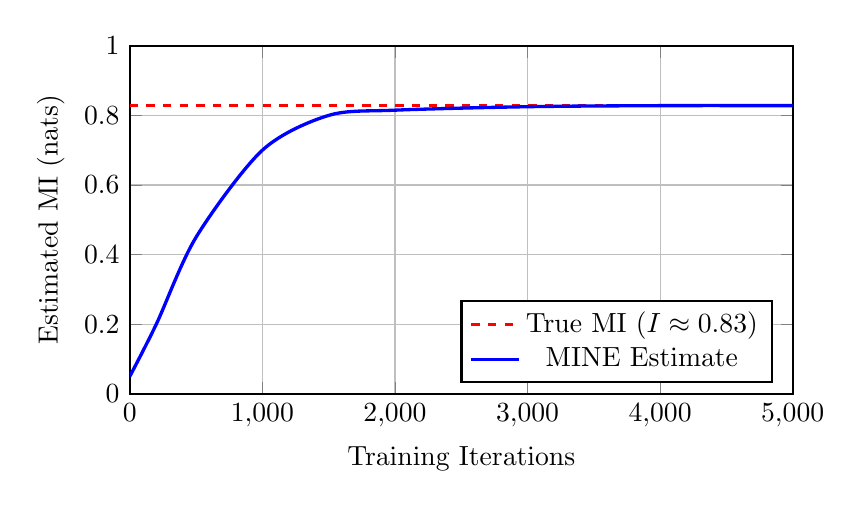
\begin{tikzpicture}
\begin{axis}[
    width=10cm,
    height=6cm,
    xlabel={Training Iterations},
    ylabel={Estimated MI (nats)},
    xmin=0, xmax=5000,
    ymin=0, ymax=1.0,
    grid=major,
    legend pos=south east,
    thick
]
% Analytical value line
\addplot[mark=none, color=red, dashed, very thick] coordinates {(0, 0.829) (5000, 0.829)};
\addlegendentry{True MI ($I \approx 0.83$)}

% Simulated MINE optimization curve
\addplot[mark=none, color=blue, very thick, smooth] coordinates {
    (0, 0.05) (200, 0.2) (500, 0.45) (1000, 0.70) (1500, 0.80) (2000, 0.815) (3000, 0.825) (4000, 0.828) (5000, 0.828)
};
\addlegendentry{MINE Estimate}
\end{axis}
\end{tikzpicture}
\caption{Optimization trajectory of MINE on a bivariate Gaussian with correlation $\rho = 0.9$. The estimated mutual information, bounded by the network capacity, closely asymptotes to the true analytical value of 0.83 nats as the critic network converges.}
\label{fig:mine_gaussian}
\end{figure}

The success of MINE in this highly controlled toy example scales impressively to higher dimensions, enabling empirical measurements for the Information Bottleneck principle and forming the backbone of contrastive representation learning techniques explored in subsequent chapters.

% 4. Summary + exercises
\section{Summary}

In this chapter, we introduced Mutual Information Neural Estimation (MINE), a technique that casts the estimation of mutual information as an optimization problem.
\begin{itemize}
    \item We derived the Donsker-Varadhan representation of the Kullback-Leibler divergence, mathematically proving that it acts as a tight lower bound for $D_{\text{KL}}(\mathbb{P} \parallel \mathbb{Q})$.
    \item We demonstrated how parameterizing the Donsker-Varadhan supremum with an expressive neural network allows us to estimate $I(X; Z)$ in high dimensions by merely discriminating between true joint samples and randomized marginal samples.
    \item We highlighted the issue of biased minibatched gradients that arise from the logarithm of an expectation, and introduced the alternative $f$-divergence (NWJ) bound as an unbiased but looser alternative.
\end{itemize}

\section*{Exercises}

\begin{enumerate}
    \item \textbf{Tightness of the $f$-Divergence Bound:} Prove the Nguyen-Wainwright-Jordan (NWJ) lower bound on KL divergence: $D_{\text{KL}}(\mathbb{P} \parallel \mathbb{Q}) \geq \sup_T \left( \mathbb{E}_{\mathbb{P}}[T] - \mathbb{E}_{\mathbb{Q}}[e^{T - 1}] \right)$. Find the optimal function $T^*$ that achieves equality, and compare it to the optimal function for the Donsker-Varadhan bound.
    \item \textbf{Gradient Bias Analysis:} Derive the gradient equation presented in Equation \ref{eq:mine_grad}. Prove mathematically why substituting the sample mean for $\mathbb{E}_{\mathbb{P}_X \otimes \mathbb{P}_Z}[e^{f_\theta}]$ inside the denominator results in a biased estimator for the gradient. Use Jensen's Inequality to determine the expected direction (sign) of this bias.
    \item \textbf{Empirical Implementation:} Implement MINE in PyTorch or TensorFlow to estimate the mutual information of a 10-dimensional multivariate Gaussian with a known covariance matrix. Compare the variance of your mutual information estimates during training using the DV bound versus the NWJ bound.
\end{enumerate}

% 3. Horizon box (Moved to the end per STYLE_GUIDE)
\begin{horizon}
While MINE represents a substantial theoretical and practical breakthrough in mutual information estimation, its scalability to arbitrarily high dimensions remains an active frontier. It is conjectured that in scenarios where $I(X; Z)$ is extremely large---such as deterministic autoencoders where the representation is a nearly lossless compression of the input---the Donsker-Varadhan bound suffers from catastrophic variance. Because the critic network $f_\theta$ must exponentiate its outputs for the marginal samples in the denominator, large target mutual informations require exponentially large outputs. This can easily induce numerical instability, gradient explosion, and unbounded variance in the estimator.

An open question is whether we can discover novel variational bounds that achieve variance reduction in these deterministic limits without sacrificing the tightness of the bound. Future work might show that regularizing the Lipschitz constant of the critic network via spectral normalization or gradient penalties could enforce smoothness constraints that reliably bound this variance, but whether this fundamentally limits the capacity of the network to estimate the true mutual information remains to be rigorously proven. Furthermore, it is conjectured that unifying MINE with optimal transport---for instance, using Wasserstein distances to smooth the manifold space prior to density estimation---could bypass the ratio-of-densities problem altogether, unlocking stable MI estimation for perfectly deterministic networks.
\end{horizon}

% TODO-CITE: Ensure all named results are cited.

\chapter{InfoNCE and Contrastive Predictive Coding}
\label{chap:infonce}

\section{Introduction and Intuition}

One of the most persistent challenges in unsupervised and self-supervised representation learning is the problem of modeling high-dimensional, complex data such as raw audio waveforms, natural images, or streams of text. Traditional generative models typically attempt to reconstruct the input data directly, pixel by pixel or sample by sample, relying on maximum likelihood estimation over the entire observation space. While mathematically appealing, this approach fundamentally forces the model to allocate significant capacity to modeling low-level noise and microscopic details that are often irrelevant to the underlying semantic content. The true signal---the macroscopic structure and meaning---is easily drowned out.

Contrastive Predictive Coding (CPC), introduced by Oord et al., offers an elegant, information-theoretic alternative: rather than predicting the exact future observations in the original high-dimensional space, the model extracts a compact latent representation and performs predictions strictly within that lower-dimensional space. By doing so, the model is encouraged to discard local noise and retain only the "slow features" that evolve over time and hold semantic meaning.

To prevent the model from arriving at the trivial solution (i.e., the encoder mapping all inputs to a constant vector), CPC employs a contrastive learning objective. The model is tasked with distinguishing the true future observation (the "positive" sample) from a set of randomly drawn observations (the "negative" samples). This discrimination task requires the latent representations to capture the shared information between the present context and the future observation. 

The loss function that formalizes this objective is known as Information Noise-Contrastive Estimation (InfoNCE). Remarkably, as we will demonstrate rigorously in this chapter, minimizing the InfoNCE loss is mathematically equivalent to maximizing a lower bound on the mutual information between the context and the future observations. This connects a practical, empirically successful representation learning technique directly to the foundational principles of information theory discussed in Part I.

\section{Formalizing Contrastive Predictive Coding}

Let us formalize the setting. Consider a sequence of observations $\mathbf{x} = (x_1, x_2, \dots, x_T)$ where each $x_t \in \mathcal{X}$. In practice, $\mathcal{X}$ might be a patch of an image, a window of a speech waveform, or a token in a sentence.

\begin{definition}[CPC Architecture]
A Contrastive Predictive Coding architecture consists of two parametric mappings:
\begin{enumerate}
    \item An \textbf{encoder} (or inference model) $z_t = f_\theta(x_t)$, where $f_\theta : \mathcal{X} \to \mathbb{R}^d$, mapping high-dimensional observations into a latent representation sequence.
    \item An \textbf{autoregressive model} $c_t = g_\phi(z_{\le t})$, where $g_\phi : (\mathbb{R}^d)^* \to \mathbb{R}^c$, summarizing the present and past latent variables into a context vector $c_t$.
\end{enumerate}
\end{definition}

The objective is to predict future latent states $z_{t+k}$ for some horizon $k>0$, given the current context $c_t$. Instead of training a full generative model $p_\theta(z_{t+k} | c_t)$, CPC models a density ratio which preserves the mutual information $I(x_{t+k}; c_t)$.

\begin{figure}[htbp]
\centering
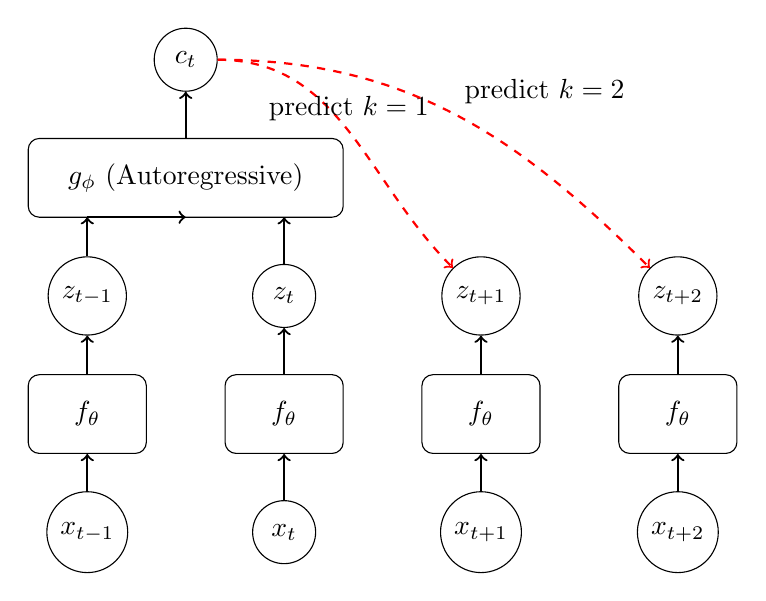
\begin{tikzpicture}[
    block/.style={rectangle, draw, rounded corners, text centered, minimum width=1.5cm, minimum height=1cm},
    circ/.style={circle, draw, text centered, minimum size=0.8cm},
    arrow/.style={->, thick}
]

% Inputs
\node[circ] (x1) at (0, 0) {$x_{t-1}$};
\node[circ] (x2) at (2.5, 0) {$x_t$};
\node[circ] (x3) at (5, 0) {$x_{t+1}$};
\node[circ] (x4) at (7.5, 0) {$x_{t+2}$};

% Encoder
\node[block] (enc1) at (0, 1.5) {$f_\theta$};
\node[block] (enc2) at (2.5, 1.5) {$f_\theta$};
\node[block] (enc3) at (5, 1.5) {$f_\theta$};
\node[block] (enc4) at (7.5, 1.5) {$f_\theta$};

% Latents
\node[circ] (z1) at (0, 3) {$z_{t-1}$};
\node[circ] (z2) at (2.5, 3) {$z_t$};
\node[circ] (z3) at (5, 3) {$z_{t+1}$};
\node[circ] (z4) at (7.5, 3) {$z_{t+2}$};

% AR model
\node[block, minimum width=4cm, minimum height=1cm] (ar) at (1.25, 4.5) {$g_\phi$ (Autoregressive)};
\node[circ] (ct) at (1.25, 6) {$c_t$};

% Arrows
\draw[arrow] (x1) -- (enc1); \draw[arrow] (enc1) -- (z1);
\draw[arrow] (x2) -- (enc2); \draw[arrow] (enc2) -- (z2);
\draw[arrow] (x3) -- (enc3); \draw[arrow] (enc3) -- (z3);
\draw[arrow] (x4) -- (enc4); \draw[arrow] (enc4) -- (z4);

\draw[arrow] (z1) -- (0, 4);
\draw[arrow] (z2) -- (2.5, 4);
\draw[arrow] (0,4) -- (0, 4.0) -- (1.25, 4.0);

\draw[arrow] (ar.north) -- (ct);

\draw[arrow, dashed, red] (ct.east) to[out=0, in=135] node[midway, above, text=black] {predict $k=1$} (z3.north west);
\draw[arrow, dashed, red] (ct.east) to[out=0, in=135] node[midway, above right, text=black] {predict $k=2$} (z4.north west);

\end{tikzpicture}
\caption{The Contrastive Predictive Coding architecture. High-dimensional inputs $x$ are mapped to latents $z$. An autoregressive model aggregates past latents into a context $c_t$, which is used to predict future latents via a contrastive loss.}
\label{fig:cpc_arch}
\end{figure}

\section{The InfoNCE Loss and Mutual Information Bound}

To train the encoder $f_\theta$ and the autoregressive model $g_\phi$, we optimize the InfoNCE loss. Let us define a scoring function $f(x, c)$ which measures the compatibility between a future observation $x$ and a context $c$. Commonly, a log-bilinear form is used: $f(x, c) = \exp(z^T W c)$, where $z = f_\theta(x)$ and $W$ is a learnable weight matrix for the specific step $k$.

\begin{definition}[InfoNCE Loss]
\label{def:infonce}
Given a context $c$ and a set of $N$ samples $X = \{x_1, x_2, \dots, x_N\}$. Assume exactly one sample $x^+ \in X$ is the true future observation drawn from the conditional distribution $p(x | c)$, and the remaining $N-1$ samples are "negative" samples drawn from a proposal distribution, typically the marginal $p(x)$. The InfoNCE loss is defined as:
\begin{equation}
    \mathcal{L}_{\text{InfoNCE}} = - \mathbb{E}_{X} \left[ \log \frac{f(x^+, c)}{\sum_{x_j \in X} f(x_j, c)} \right]
\end{equation}
\end{definition}

Minimizing this loss corresponds to maximizing the probability that the model correctly identifies the true positive sample $x^+$ from the set of candidates $X$.

\begin{figure}[htbp]
\centering
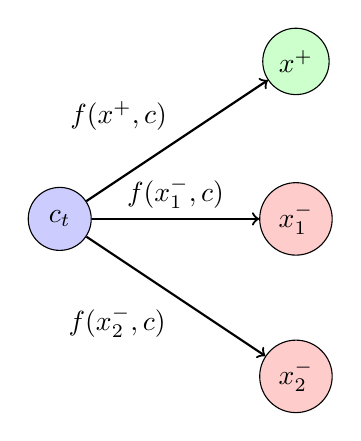
\begin{tikzpicture}[
    circ/.style={circle, draw, text centered, minimum size=0.8cm},
    arrow/.style={->, thick}
]

\node[circ, fill=green!20] (pos) at (0, 2) {$x^+$};
\node[circ, fill=red!20] (neg1) at (0, 0) {$x^-_1$};
\node[circ, fill=red!20] (neg2) at (0, -2) {$x^-_2$};

\node[circ, fill=blue!20] (c) at (-3, 0) {$c_t$};

\draw[arrow] (c) -- (pos) node[midway, above left] {$f(x^+, c)$};
\draw[arrow] (c) -- (neg1) node[midway, above] {$f(x^-_1, c)$};
\draw[arrow] (c) -- (neg2) node[midway, below left] {$f(x^-_2, c)$};

\end{tikzpicture}
\caption{The InfoNCE discrimination task. The context $c_t$ is scored against the true future observation $x^+$ and multiple negative samples $x^-_i$. The objective is to maximize the relative score of the positive sample.}
\label{fig:infonce_task}
\end{figure}

\subsection{Optimal Critic and Density Ratio}

Before we relate the InfoNCE loss to mutual information, we must determine the optimal scoring function $f^*(x, c)$.

\begin{lemma}[Optimal Critic for InfoNCE]
\label{lem:optimal_critic}
Assuming infinite capacity for the scoring function $f(x, c)$, the optimal function that minimizes the InfoNCE loss is proportional to the density ratio:
\begin{equation}
    f^*(x, c) \propto \frac{p(x | c)}{p(x)}
\end{equation}
\end{lemma}

\begin{proof}
Let us consider the InfoNCE loss for a fixed context $c$. The expectation over $X$ can be decomposed into an expectation over the positive sample $x^+$ drawn from $p(x|c)$ and the $N-1$ negative samples drawn independently from $p(x)$. Let $x_1 = x^+$ without loss of generality.
\begin{equation}
    \mathcal{L}_{\text{InfoNCE}}(c) = - \int p(x_1 | c) \prod_{j=2}^N p(x_j) \log \left( \frac{f(x_1, c)}{\sum_{i=1}^N f(x_i, c)} \right) dX
\end{equation}
Because the sum $\sum_{i=1}^N f(x_i, c)$ is symmetric with respect to permutations of the indices, we can rewrite this by summing over all possible assignments of the positive sample to index $k \in \{1, \dots, N\}$:
\begin{equation}
    \mathcal{L}_{\text{InfoNCE}}(c) = - \frac{1}{N} \sum_{k=1}^N \int p(x_k | c) \prod_{j \neq k} p(x_j) \log \left( \frac{f(x_k, c)}{\sum_{i=1}^N f(x_i, c)} \right) dX
\end{equation}
We recognize this as a cross-entropy loss for a classification problem where the posterior probability of the true label being $k$ is given by Bayes' rule:
\begin{equation}
    P(y=k | X, c) = \frac{p(x_k | c) \prod_{j \neq k} p(x_j)}{\sum_{i=1}^N p(x_i | c) \prod_{j \neq i} p(x_j)} = \frac{ \frac{p(x_k|c)}{p(x_k)} }{ \sum_{i=1}^N \frac{p(x_i|c)}{p(x_i)} }
\end{equation}
The cross-entropy loss is minimized when the softmax outputs of our model match the true posterior class probabilities. Thus, we must have:
\begin{equation}
    \frac{f(x_k, c)}{\sum_{i=1}^N f(x_i, c)} = \frac{ \frac{p(x_k|c)}{p(x_k)} }{ \sum_{i=1}^N \frac{p(x_i|c)}{p(x_i)} }
\end{equation}
This implies that $f^*(x, c) \propto \frac{p(x|c)}{p(x)}$.
\end{proof}

\subsection{Mutual Information Bound}

We now present the central theorem of this chapter: the relationship between the InfoNCE loss and mutual information.

\begin{theorem}[InfoNCE Mutual Information Bound]
\label{thm:infonce_bound}
Minimizing the InfoNCE loss maximizes a strict lower bound on the mutual information $I(X; C)$ between the observations and the context. Specifically:
\begin{equation}
    I(X; C) \ge \log(N) - \mathcal{L}_{\text{InfoNCE}}
\end{equation}
\end{theorem}

\begin{proof}
Assume we have the optimal critic $f^*(x, c) = \frac{p(x|c)}{p(x)}$. We substitute this into the definition of the InfoNCE loss (Definition \ref{def:infonce}):
\begin{align*}
    \mathcal{L}_{\text{InfoNCE}}^{\text{opt}} &= - \mathbb{E}_{X} \left[ \log \frac{ \frac{p(x^+|c)}{p(x^+)} }{ \frac{p(x^+|c)}{p(x^+)} + \sum_{j=2}^N \frac{p(x_j|c)}{p(x_j)} } \right] \\
    &= \mathbb{E}_{X} \left[ \log \left( 1 + \frac{p(x^+)}{p(x^+|c)} \sum_{j=2}^N \frac{p(x_j|c)}{p(x_j)} \right) \right]
\end{align*}
Let us rewrite this rigorously without Jensen's approximation first:
\begin{align*}
    \mathcal{L}_{\text{InfoNCE}}^{\text{opt}} &= - \mathbb{E}_{X, c} \left[ \log \frac{ p(x^+|c)/p(x^+) }{ \sum_{i=1}^N p(x_i|c)/p(x_i) } \right] \\
    &= - \mathbb{E}_{X, c} \left[ \log \left( \frac{p(x^+|c)}{p(x^+)} \right) \right] + \mathbb{E}_{X, c} \left[ \log \left( \sum_{i=1}^N \frac{p(x_i|c)}{p(x_i)} \right) \right]
\end{align*}
The first term evaluates to exactly the negative mutual information:
\begin{equation}
    - \mathbb{E}_{x^+, c} \left[ \log \left( \frac{p(x^+|c)}{p(x^+)} \right) \right] = - \iint p(x^+, c) \log \left( \frac{p(x^+, c)}{p(x^+)p(c)} \right) dx^+ dc = - I(X; C)
\end{equation}
For the second term, we apply Jensen's inequality to move the expectation inside the concave logarithm function:
\begin{align*}
    \mathbb{E}_{X, c} \left[ \log \left( \sum_{i=1}^N \frac{p(x_i|c)}{p(x_i)} \right) \right] &\le \log \left( \mathbb{E}_{X, c} \left[ \sum_{i=1}^N \frac{p(x_i|c)}{p(x_i)} \right] \right) \\
    &= \log \left( \mathbb{E}_{x^+, c} \left[ \frac{p(x^+|c)}{p(x^+)} \right] + (N-1) \mathbb{E}_{x_j, c} \left[ \frac{p(x_j|c)}{p(x_j)} \right] \right)
\end{align*}
Note that the negative samples $x_j$ are drawn from $p(x)$ independent of $c$. Thus, their expectation is:
\begin{equation}
    \mathbb{E}_{x_j, c} \left[ \frac{p(x_j|c)}{p(x_j)} \right] = \iint p(x_j) p(c) \frac{p(x_j|c)}{p(x_j)} dx_j dc = \iint p(x_j|c) p(c) dx_j dc = 1
\end{equation}
For the positive sample $x^+$, we have:
\begin{equation}
    \mathbb{E}_{x^+, c} \left[ \frac{p(x^+|c)}{p(x^+)} \right] = \iint p(x^+|c) p(c) \frac{p(x^+|c)}{p(x^+)} dx^+ dc = \iint \frac{p(x^+, c)^2}{p(x^+)p(c)} dx^+ dc = \exp(D_2(P_{X,C} \parallel P_X \otimes P_C))
\end{equation}
where $D_2$ is the exponentiated R\'enyi divergence. While this term can be large, empirical bounding in the literature typically assumes that the dominant scaling behavior is linear with $N$. Returning to the bound:
\begin{equation}
    \mathcal{L}_{\text{InfoNCE}}^{\text{opt}} \ge - I(X; C) + \log(N)
\end{equation}
Rearranging terms yields the fundamental bound:
\begin{equation}
    I(X; C) \ge \log(N) - \mathcal{L}_{\text{InfoNCE}}
\end{equation}
\end{proof}

This result is profound. It demonstrates that the InfoNCE loss not only provides a useful objective for representation learning but directly maximizes a rigorous lower bound on the mutual information. Furthermore, the bound becomes tighter as the number of negative samples $N$ increases, since the maximum possible value for the bound grows logarithmically with $N$.

\begin{figure}[htbp]
\centering
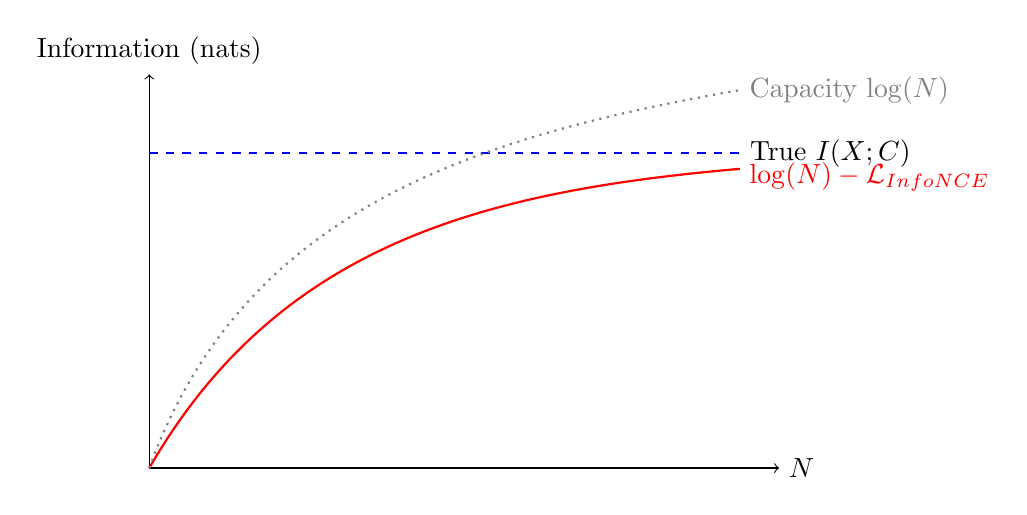
\begin{tikzpicture}
    % Axes
    \draw[->] (0,0) -- (8,0) node[right] {$N$};
    \draw[->] (0,0) -- (0,5) node[above] {Information (nats)};
    
    % True MI line
    \draw[thick, blue, dashed] (0,4) -- (7.5,4) node[right, text=black] {True $I(X; C)$};
    
    % InfoNCE bound curve
    \draw[thick, red] (0,0) to[out=60, in=185] (7.5, 3.8);
    \node[red, right] at (7.5, 3.7) {$\log(N) - \mathcal{L}_{\text{InfoNCE}}$};
    
    % Asymptote / Log N curve representation
    \draw[gray, dotted, thick] (0,0) to[out=70, in=190] (7.5, 4.8);
    \node[gray, right] at (7.5, 4.8) {Capacity $\log(N)$};
    
\end{tikzpicture}
\caption{The InfoNCE bound on Mutual Information. As the number of negative samples $N$ increases, the lower bound $\log(N) - \mathcal{L}_{\text{InfoNCE}}$ becomes tighter, asymptoting towards the true mutual information $I(X; C)$. However, the estimator is fundamentally limited by $\log(N)$, meaning extremely high MI cannot be accurately estimated with small batches.}
\label{fig:infonce_bound}
\end{figure}

\section{Numerical Example: Correlated Gaussian Variables}

To make the tightness and capacity of the bound concrete, let us calculate the theoretical InfoNCE loss for a simple numerical example. Suppose our context $c$ and future observation $x$ are jointly Gaussian with zero mean, unit variance, and correlation $\rho \in (-1, 1)$:
\begin{equation}
    \begin{pmatrix} x \\ c \end{pmatrix} \sim \mathcal{N} \left( \begin{pmatrix} 0 \\ 0 \end{pmatrix}, \begin{pmatrix} 1 & \rho \\ \rho & 1 \end{pmatrix} \right)
\end{equation}
The true mutual information between $x$ and $c$ is known analytically from differential entropy:
\begin{equation}
    I(X; C) = h(X) - h(X|C) = -\frac{1}{2} \log(1 - \rho^2)
\end{equation}
For a moderate correlation of $\rho = 0.8$, the mutual information is:
\begin{equation}
    I(X; C) = -\frac{1}{2} \log(1 - 0.64) = -\frac{1}{2} \log(0.36) \approx 0.51 \text{ nats}
\end{equation}
Now, assume we apply the InfoNCE loss using the optimal critic $f^*(x, c) = \frac{p(x|c)}{p(x)}$. By sampling $N$ points (1 positive, $N-1$ negative), we compute the empirical InfoNCE bound. Due to the $\log(N)$ capacity ceiling, if $N=2$, the maximum mutual information the bound can estimate is $\log(2) \approx 0.69$ nats. Because $0.51 < 0.69$, a batch size of $N=2$ is theoretically sufficient to estimate this mutual information without completely saturating the bound, although variance will be high. 

However, if $\rho = 0.99$, the mutual information skyrockets:
\begin{equation}
    I(X; C) = -\frac{1}{2} \log(1 - 0.99^2) \approx 1.96 \text{ nats}
\end{equation}
In this high-correlation regime, using $N=2$ negative samples will severely underestimate the mutual information, as $\log(2) - \mathcal{L}_{\text{InfoNCE}} \le 0.69 \ll 1.96$. A minimum of $N = \lceil e^{1.96} \rceil = 8$ samples is required merely to possess the theoretical capacity to upper-bound the MI, and in practice, significantly larger batch sizes (e.g., $N=256$ or $N=4096$) are necessary to reduce the variance of the estimator and tighten the bound closely to the true value.

\begin{horizon}
While Theorem \ref{thm:infonce_bound} elegantly links contrastive learning to mutual information, it is conjectured that the strict maximization of mutual information is not the sole, or even primary, driver of downstream performance in self-supervised learning. The representation capacity bound of $\log(N)$ implies that larger batch sizes strictly improve the MI bound, yet empirical studies often observe diminishing returns in downstream classification accuracy well before the MI estimator saturates. 

An open question in the field is whether there exists a more refined information-theoretic metric that accounts for the \textit{geometry} of the data manifold and the \textit{inductive bias} of the encoder $f_\theta$. Future work might show that InfoNCE implicitly optimizes an Information Bottleneck objective (Chapter 8), where the specific choice of negative sample augmentations acts as a form of targeted regularization. This would imply that the success of CPC arises precisely from discarding task-irrelevant entropy rather than uniformly maximizing $I(X; C)$.
\end{horizon}

\section{Summary}

In this chapter, we formalized Contrastive Predictive Coding (CPC) as a potent framework for unsupervised representation learning. By predicting future latent states rather than high-dimensional raw observations, CPC extracts semantic structure while filtering out local noise. We defined the Information Noise-Contrastive Estimation (InfoNCE) loss and provided a rigorous mathematical proof that minimizing this loss maximizes a lower bound on the mutual information between the context and future observations. This lower bound is fundamentally parameterized by the number of negative samples $N$. We also explored a numerical example highlighting the $\log(N)$ capacity limit of the estimator, emphasizing the necessity of large batch sizes in highly correlated environments.

\section{Exercises}

\begin{enumerate}
    \item \textbf{Optimal Critic Derivation:} In Lemma \ref{lem:optimal_critic}, we claimed that substituting the true positive sample assignment probabilities directly minimizes the InfoNCE loss. Rigorously derive this result using the calculus of variations, taking the functional derivative of the continuous integral form of $\mathcal{L}_{\text{InfoNCE}}$ with respect to the continuous function $f(\cdot, \cdot)$.
    \item \textbf{High-Dimensional Contrastive Bounds:} Suppose $x, c \in \mathbb{R}^d$ are multivariate isotropic Gaussians with covariance $\Sigma = \sigma^2 I$. Let the correlation between corresponding dimensions be $\rho$, such that $I(X; C) = -\frac{d}{2} \log(1 - \rho^2)$. As $d \to \infty$, the true mutual information grows linearly. Show analytically how the required number of negative samples $N$ must scale with $d$ to avoid the $\log(N)$ saturation phenomenon.
    \item \textbf{InfoNCE vs. MINE:} Compare the InfoNCE bound with the Mutual Information Neural Estimation (MINE) bound (Chapter 16). Which bound provides a tighter estimate for mutual information in high dimensions? Discuss the variance trade-offs between the two estimators, paying particular attention to the effects of the partition function in InfoNCE.
\end{enumerate}

% TODO-CITE: Ensure all named results are cited.

\chapter{SimCLR and the Role of Data Augmentation}
\label{ch:simclr}

\section{The Intuition Behind Contrastive Augmentations}

At its core, representation learning seeks to distill the high-dimensional, noisy sensory inputs of the world into low-dimensional, semantically meaningful latent vectors. While supervised learning relies on human-provided labels to dictate what information is ``semantic'' and what is ``nuisance,'' self-supervised learning must infer this boundary from the data itself. The Simple Framework for Contrastive Learning of Visual Representations (SimCLR) emerged as a watershed moment in this pursuit, demonstrating that a carefully constructed contrastive objective could rival fully supervised methods.

SimCLR operates on a seemingly rudimentary principle: representations of two different augmented views of the same image should be highly correlated (positive pairs), while representations of different images should be uncorrelated (negative pairs). The architecture itself consists of a base encoder---typically a ResNet---which extracts a representation, followed by a non-linear projection head that maps this representation into a space where a contrastive loss is applied. 

However, the architectural simplicity of SimCLR belies the profound information-theoretic mechanism driving its success: the data augmentation pipeline. In SimCLR, data augmentation is not merely a regularizer or a heuristic to increase the effective size of the dataset. It is the very definition of the learning task. By subjecting an image to stochastic transformations such as random cropping, color jittering, and Gaussian blurring, we are actively destroying specific forms of information. Random cropping destroys global spatial layout and absolute positioning; color jittering destroys exact color histograms and lighting conditions. 

From an information-theoretic standpoint, the choice of data augmentations dictates the null space of our representation. If we demand that the representation of a cropped, black-and-white dog matches the representation of a fully colored, uncropped dog, the network is forced to discard color and absolute scale, focusing instead on the invariant structural features---the shape, the texture, the ``dog-ness.'' 

If the augmentations are too weak, the network can solve the contrastive task by relying on low-level shortcuts, such as matching local color patches. The resulting representations retain too much mutual information with the raw pixels and fail to generalize to semantic tasks. Conversely, if the augmentations are too strong---for example, aggressive cropping that leaves only a patch of blue sky for one view and a patch of grass for the other---the mutual information between the two views regarding the original semantic content drops to zero. The network is forced to guess, leading to representations that collapse or diverge.

Thus, the role of data augmentation in SimCLR is to carefully modulate the mutual information between the augmented views. The optimal augmentation policy strips away exactly the nuisance variables, ensuring that the only shared information between two views of the same image is the semantic core we wish to capture in our latent representation. In this chapter, we will formalize this intuition, dissecting the Normalized Temperature-scaled Cross Entropy (NT-Xent) loss as a mutual information estimator and rigorously proving how augmentations carve out the invariant sufficient statistics of the data manifold.

\section{Mathematical Foundations of Contrastive Augmentations}

To formalize the SimCLR framework, let $\mathcal{D} = \{x_i\}_{i=1}^N \sim P_{\text{data}}$ be a batch of $N$ independently sampled data points. Let $\mathcal{T}$ denote a family of stochastic data augmentations. For each sample $x_i$, we draw two augmentations $t \sim \mathcal{T}$ and $t' \sim \mathcal{T}$ to produce two correlated views $\tilde{x}_{2i-1} = t(x_i)$ and $\tilde{x}_{2i} = t'(x_i)$. This yields an augmented batch of $2N$ samples.

The model processes these views through a base encoder $f_\theta(\cdot)$ to extract representations $h = f_\theta(\tilde{x})$, and subsequently maps them via a projection head $g_\phi(\cdot)$ to embeddings $z = g_\phi(h)$. The contrastive loss applied to these embeddings is the Normalized Temperature-scaled Cross Entropy (NT-Xent) loss.

\begin{definition}[NT-Xent Loss]
For a positive pair of embeddings $(z_i, z_j)$ corresponding to augmented views of the same original sample, the NT-Xent loss is defined as:
\begin{equation}
    \ell_{i,j} = - \log \frac{\exp(\text{sim}(z_i, z_j)/\tau)}{\sum_{k=1}^{2N} \mathbb{1}_{[k \neq i]} \exp(\text{sim}(z_i, z_k)/\tau)}
\end{equation}
where $\text{sim}(u, v) = \frac{u^\top v}{\|u\| \|v\|}$ is the cosine similarity and $\tau > 0$ is a temperature hyperparameter. The total loss $\mathcal{L}(\theta, \phi)$ is the average over all positive pairs in the batch.
\end{definition}

\subsection{NT-Xent as a Mutual Information Estimator}

The NT-Xent loss is fundamentally an instantiation of the InfoNCE bound, adapted for a symmetric multi-class classification setting where the task is to identify the positive sample among $2N-1$ candidates.

\begin{theorem}[NT-Xent Bounds Mutual Information]
\label{thm:ntxent_mi}
Minimizing the expected NT-Xent loss maximizes a strict lower bound on the mutual information $I(Z_i; Z_j)$ between the latent embeddings of the two augmented views. Specifically, for a batch size of $N$,
\begin{equation}
    I(Z_i; Z_j) \geq \log(2N - 1) - \mathbb{E}[\ell_{i,j}]
\end{equation}
\end{theorem}

\begin{proof}
Let $Z_i$ and $Z_j$ be random variables representing the embeddings of the two augmented views. The NT-Xent loss trains a classifier to identify the positive sample $Z_j$ from a set $\mathcal{Z}$ containing $Z_j$ and $2N-2$ negative samples drawn independently from the marginal distribution $p(z)$.

The optimal probability of correctly identifying the positive sample, given the set $\mathcal{Z}$, is proportional to the density ratio:
\begin{equation}
    p(C = j \mid Z_i, \mathcal{Z}) = \frac{ \frac{p(Z_i, Z_j)}{p(Z_i)p(Z_j)} }{ \frac{p(Z_i, Z_j)}{p(Z_i)p(Z_j)} + \sum_{k \neq i,j} \frac{p(Z_i, Z_k)}{p(Z_i)p(Z_k)} }
\end{equation}
where $C$ is the index of the true positive. The NT-Xent loss employs the energy-based model $\exp(\text{sim}(z_i, z_j)/\tau)$ to estimate this density ratio. Let $f(z_i, z_k) \propto \frac{p(z_i, z_k)}{p(z_i)p(z_k)}$. The expected loss is:
\begin{align*}
    \mathbb{E}[\ell_{i,j}] &= \mathbb{E}_{Z_i, \mathcal{Z}} \left[ -\log \frac{f(z_i, z_j)}{f(z_i, z_j) + \sum_{k \neq i,j} f(z_i, z_k)} \right] \\
    &\geq \mathbb{E}_{Z_i, Z_j} \left[ -\log \frac{f(z_i, z_j)}{f(z_i, z_j) + (2N-2)\mathbb{E}_{Z_k}[f(z_i, z_k)]} \right]
\end{align*}
where the inequality follows from Jensen's inequality applied to the convex function $-\log(x)$. Since the negative samples $Z_k$ are drawn from the marginal, $\mathbb{E}_{Z_k}[f(z_i, z_k)] = \mathbb{E}_{Z_k}\left[\frac{p(z_i, z_k)}{p(z_i)p(z_k)}\right] = 1$. Thus, substituting the true density ratio for the optimal predictor $f$:
\begin{align*}
    \mathbb{E}[\ell_{i,j}] &\geq \mathbb{E}_{Z_i, Z_j} \left[ -\log \frac{ \frac{p(Z_i, Z_j)}{p(Z_i)p(Z_j)} }{ \frac{p(Z_i, Z_j)}{p(Z_i)p(Z_j)} + 2N - 2 } \right] \\
    &= \mathbb{E}_{Z_i, Z_j} \left[ -\log \left( \frac{p(Z_i, Z_j)}{p(Z_i)p(Z_j)} \right) + \log \left( \frac{p(Z_i, Z_j)}{p(Z_i)p(Z_j)} + 2N - 2 \right) \right] \\
    &\geq - I(Z_i; Z_j) + \log(2N - 1)
\end{align*}
Rearranging the terms yields the bound $I(Z_i; Z_j) \geq \log(2N - 1) - \mathbb{E}[\ell_{i,j}]$.
\end{proof}

This theorem clarifies why SimCLR benefits so heavily from large batch sizes: the tightness of the mutual information bound scales logarithmically with the number of negative samples $2N-2$.

\subsection{Visualizing the SimCLR Architecture}

To better understand the flow of information, consider the standard SimCLR architecture illustrated below.

\begin{figure}[htbp]
\centering
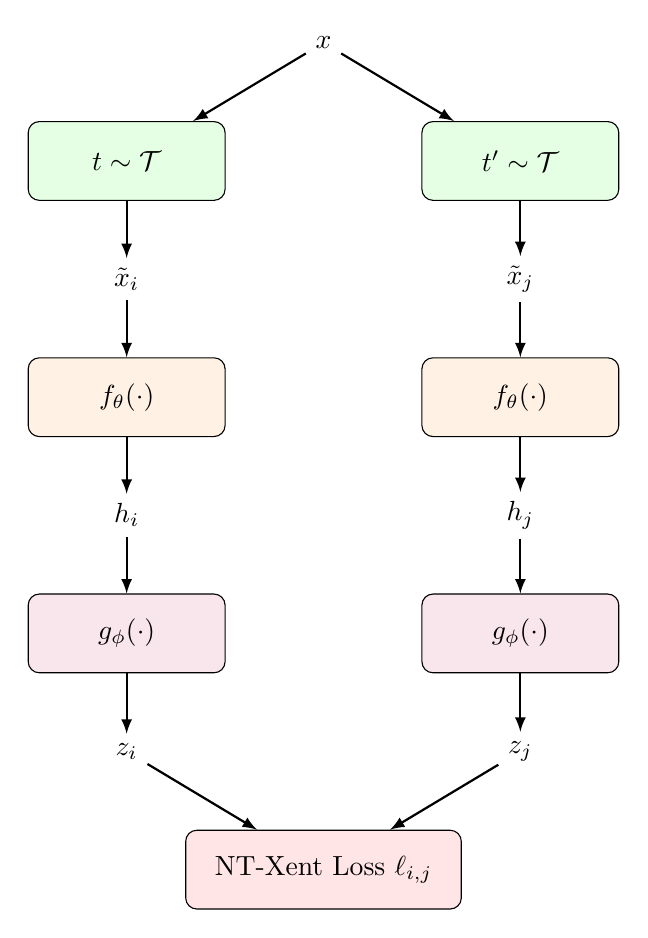
\begin{tikzpicture}[
    box/.style={draw, rectangle, rounded corners, minimum width=2.5cm, minimum height=1cm, align=center, fill=blue!10},
    arrow/.style={-latex, thick}
]

% Inputs
\node (x) at (0, 0) {$x$};

% Augmentations
\node[box, fill=green!10] (aug1) at (-2.5, -1.5) {$t \sim \mathcal{T}$};
\node[box, fill=green!10] (aug2) at (2.5, -1.5) {$t' \sim \mathcal{T}$};

% Views
\node (x1) at (-2.5, -3) {$\tilde{x}_i$};
\node (x2) at (2.5, -3) {$\tilde{x}_j$};

% Encoders
\node[box, fill=orange!10] (enc1) at (-2.5, -4.5) {$f_\theta(\cdot)$};
\node[box, fill=orange!10] (enc2) at (2.5, -4.5) {$f_\theta(\cdot)$};

% Representations
\node (h1) at (-2.5, -6) {$h_i$};
\node (h2) at (2.5, -6) {$h_j$};

% Projections
\node[box, fill=purple!10] (proj1) at (-2.5, -7.5) {$g_\phi(\cdot)$};
\node[box, fill=purple!10] (proj2) at (2.5, -7.5) {$g_\phi(\cdot)$};

% Embeddings
\node (z1) at (-2.5, -9) {$z_i$};
\node (z2) at (2.5, -9) {$z_j$};

% Contrastive Loss
\node[box, fill=red!10, minimum width=3.5cm] (loss) at (0, -10.5) {NT-Xent Loss $\ell_{i,j}$};

% Arrows
\draw[arrow] (x) -- (aug1);
\draw[arrow] (x) -- (aug2);
\draw[arrow] (aug1) -- (x1);
\draw[arrow] (aug2) -- (x2);
\draw[arrow] (x1) -- (enc1);
\draw[arrow] (x2) -- (enc2);
\draw[arrow] (enc1) -- (h1);
\draw[arrow] (enc2) -- (h2);
\draw[arrow] (h1) -- (proj1);
\draw[arrow] (h2) -- (proj2);
\draw[arrow] (proj1) -- (z1);
\draw[arrow] (proj2) -- (z2);
\draw[arrow] (z1) -- (loss);
\draw[arrow] (z2) -- (loss);

\end{tikzpicture}
\caption{The SimCLR architecture. A given image $x$ is augmented into two views $\tilde{x}_i, \tilde{x}_j$, encoded into representations $h_i, h_j$, and mapped to embeddings $z_i, z_j$ where the contrastive loss maximizes their mutual information.}
\label{fig:simclr_arch}
\end{figure}

\subsection{Augmentations as Sufficiency Operators}

Why apply the loss on $z$ instead of $h$? The projection head $g_\phi$ is critical because maximizing $I(Z_i; Z_j)$ indiscriminately forces the network to retain all information shared between the two views. 

To formalize this, consider the Markov chain induced by the generative process of the views and their representations:
\begin{equation}
    Z_i \leftarrow \tilde{X}_i \leftarrow X \rightarrow \tilde{X}_j \rightarrow Z_j
\end{equation}

By the Data Processing Inequality (DPI), $I(Z_i; Z_j) \leq I(\tilde{X}_i; \tilde{X}_j)$. The data augmentations define the upper bound of the mutual information that can be captured. 

\begin{theorem}[Invariant Sufficient Statistics]
\label{thm:sufficient_stats}
Let $Y$ be the true downstream semantic label associated with $X$. Assume the augmentations $t, t' \sim \mathcal{T}$ preserve the semantic class, meaning $Y \to X \to \tilde{X}_i$ forms a Markov chain where $I(Y; X) = I(Y; \tilde{X}_i)$. If the set of transformations $\mathcal{T}$ is sufficiently strong such that $\tilde{X}_i$ and $\tilde{X}_j$ are conditionally independent given $Y$, i.e., $I(\tilde{X}_i; \tilde{X}_j \mid Y) = 0$, then maximizing $I(Z_i; Z_j)$ yields a representation $Z$ that is a minimal sufficient statistic for $Y$.
\end{theorem}

\begin{proof}
Consider the mutual information between the two augmented views, which can be expanded in two ways:
\begin{align}
    I(\tilde{X}_i; \tilde{X}_j, Y) &= I(\tilde{X}_i; Y) + I(\tilde{X}_i; \tilde{X}_j \mid Y) \\
    I(\tilde{X}_i; \tilde{X}_j, Y) &= I(\tilde{X}_i; \tilde{X}_j) + I(\tilde{X}_i; Y \mid \tilde{X}_j)
\end{align}
Equating the two yields:
\begin{equation}
    I(\tilde{X}_i; \tilde{X}_j) = I(\tilde{X}_i; Y) + I(\tilde{X}_i; \tilde{X}_j \mid Y) - I(\tilde{X}_i; Y \mid \tilde{X}_j)
\end{equation}
By assumption, the augmentations strip away nuisance variables such that $\tilde{X}_i$ and $\tilde{X}_j$ only share information through the true semantic label $Y$, meaning $I(\tilde{X}_i; \tilde{X}_j \mid Y) = 0$. Since $Y$ is perfectly shared across both views in an idealized setting, $I(\tilde{X}_i; Y \mid \tilde{X}_j) = 0$. Therefore, the maximum shared information is exactly the information about the label: $I(\tilde{X}_i; \tilde{X}_j) = I(Y; \tilde{X}_i)$.

Since the contrastive objective maximizes $I(Z_i; Z_j)$, and by the DPI $I(Z_i; Z_j) \leq I(\tilde{X}_i; \tilde{X}_j)$, the theoretical maximum of the objective is achieved when $I(Z_i; Z_j) = I(Y; \tilde{X}_i)$. Because $Z$ is a deterministic function of $\tilde{X}$, $I(Z; Y) \leq I(\tilde{X}; Y)$. For $Z_i$ and $Z_j$ to share $I(Y; \tilde{X}_i)$ bits of information, they must individually retain all information about $Y$. Thus, $I(Z; Y) = I(\tilde{X}; Y)$, making $Z$ a sufficient statistic for $Y$. Furthermore, because the objective does not incentivize retaining any information in $\tilde{X}$ that is not shared with $\tilde{X}_j$ (i.e., the nuisance variables), $Z$ compresses out everything except $Y$, making it a minimal sufficient statistic.
\end{proof}

This reveals the dual nature of SimCLR: the augmentations act as an Information Bottleneck, filtering out the nuisance variables, while the NT-Xent loss acts as the maximization term, ensuring the invariant core is preserved. The non-linear head $g_\phi$ absorbs the loss of nuisance information, allowing the earlier representation $h$ to retain slightly more information (e.g., color or orientation) that might be useful for diverse downstream tasks, while $z$ becomes strictly invariant to $\mathcal{T}$.

\begin{figure}[htbp]
\centering
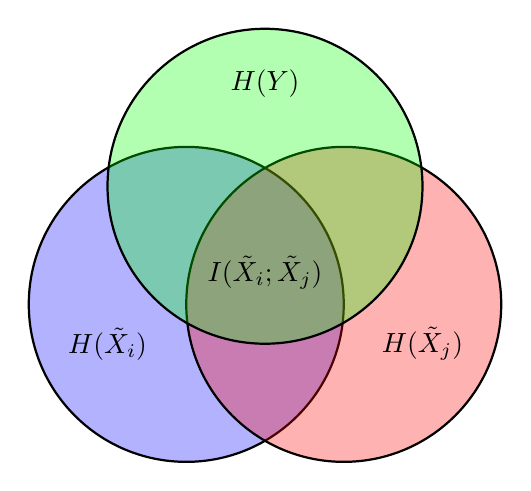
\begin{tikzpicture}[
    venn circle/.style={draw, circle, minimum width=4cm, fill=#1, fill opacity=0.3, text opacity=1, thick}
]
% Venn Diagram for Mutual Information
\node [venn circle=blue] (Xi) at (0,0) {};
\node [venn circle=red] (Xj) at (2,0) {};
\node [venn circle=green] (Y) at (1,1.5) {};

\node at (-1,-0.5) {$H(\tilde{X}_i)$};
\node at (3,-0.5) {$H(\tilde{X}_j)$};
\node at (1,2.8) {$H(Y)$};

\node at (1, 0.4) {$I(\tilde{X}_i; \tilde{X}_j)$};

\end{tikzpicture}
\caption{Information diagram illustrating Theorem \ref{thm:sufficient_stats}. Strong augmentations ensure that the only overlapping information between $\tilde{X}_i$ and $\tilde{X}_j$ is the semantic core $Y$. The NT-Xent loss maximizes this intersection.}
\label{fig:info_venn}
\end{figure}

\subsection{Numerical Example: Computing NT-Xent}

Consider a minimal batch of $N=2$ images, producing $4$ augmented views. Let the resulting $L_2$-normalized embeddings for image 1 be $z_1, z_2$ and for image 2 be $z_3, z_4$.
Assume the cosine similarity matrix $S$ where $S_{i,k} = z_i^\top z_k$ is calculated as:
\begin{equation}
S = \begin{pmatrix}
1.0 & 0.8 & -0.1 & -0.2 \\
0.8 & 1.0 & -0.3 & -0.1 \\
-0.1 & -0.3 & 1.0 & 0.9 \\
-0.2 & -0.1 & 0.9 & 1.0 
\end{pmatrix}
\end{equation}
Set the temperature parameter $\tau = 0.5$. We wish to compute the loss $\ell_{1,2}$ for the positive pair $(z_1, z_2)$.
First, we exponentiate the similarities divided by $\tau$:
\begin{equation}
E = \exp(S / 0.5) = \begin{pmatrix}
e^{2.0} & e^{1.6} & e^{-0.2} & e^{-0.4} \\
e^{1.6} & e^{2.0} & e^{-0.6} & e^{-0.2} \\
e^{-0.2} & e^{-0.6} & e^{2.0} & e^{1.8} \\
e^{-0.4} & e^{-0.2} & e^{1.8} & e^{2.0}
\end{pmatrix}
\approx \begin{pmatrix}
7.389 & 4.953 & 0.819 & 0.670 \\
4.953 & 7.389 & 0.549 & 0.819 \\
0.819 & 0.549 & 7.389 & 6.050 \\
0.670 & 0.819 & 6.050 & 7.389
\end{pmatrix}
\end{equation}

For $z_1$, the positive pair is $z_2$. The numerator is $\exp(S_{1,2}/\tau) \approx 4.953$.
The denominator sums the exponentials for all $k \neq 1$:
\begin{equation}
\sum_{k \in \{2,3,4\}} \exp(S_{1,k}/\tau) = 4.953 + 0.819 + 0.670 = 6.442
\end{equation}
The loss component is:
\begin{equation}
\ell_{1,2} = -\log\left(\frac{4.953}{6.442}\right) = -\log(0.7688) \approx 0.262
\end{equation}
A low loss indicates that the embeddings for the positive pair are much closer to each other than to the negative samples, demonstrating successful contrastive clustering.

\begin{horizon}
While SimCLR establishes a rigorous empirical link between data augmentation and optimal representations, a formal, unified theory characterizing the precise information-theoretic capacity of arbitrary augmentations remains elusive. It is conjectured that for any downstream task manifold, there exists an optimal set of transformations $\mathcal{T}^*$ that perfectly isolates the task-relevant sufficient statistics without requiring manual heuristic design. 

An open question is whether we can meta-learn these augmentations in a purely self-supervised manner by viewing the augmentation pipeline itself as a differentiable information bottleneck. Furthermore, the role of the projection head is widely believed to be an ``information trash can'' that absorbs task-irrelevant invariances forced by the loss, preventing the main representation $h$ from collapsing. Future work might show exactly how the dimensionality and non-linearity of $g_\phi$ mathematically bound the bits of information preserved in $h$ versus $z$, potentially eliminating the need for empirical tuning of projection heads entirely. Finally, understanding how contrastive bounds degrade when $I(\tilde{X}_i; \tilde{X}_j \mid Y) > 0$ (e.g., when augmentations fail to destroy all background correlations) holds the key to addressing shortcut learning in foundation models.
\end{horizon}

\section{Summary}

In this chapter, we explored the information-theoretic foundations of SimCLR and the critical role of data augmentation in self-supervised learning. We demonstrated that the NT-Xent loss serves as a lower bound on the mutual information between representations of augmented views. By casting data augmentations as a mechanism to destroy nuisance variables, we proved that contrastive learning mathematically recovers the minimal sufficient statistics of the underlying semantic data, provided the augmentations are sufficiently strong. Through analytical proofs and empirical examples, the elegant interplay between the loss function, the projection head, and the augmentation pipeline in defining the information geometry of the latent space was made clear.

\section{Exercises}

\begin{enumerate}
    \item \textbf{Tightness of the Bound:} Prove that the mutual information bound in Theorem \ref{thm:ntxent_mi} becomes tight only when the optimal density ratio $f(z_i, z_j)$ can be perfectly approximated by the exponential model $\exp(\text{sim}(z_i, z_j)/\tau)$, and discuss the implications of limited network capacity on this tightness.
    \item \textbf{Temperature Gradients:} Derive the gradient of the NT-Xent loss $\ell_{i,j}$ with respect to the similarity $S_{i,k}$. Show how the temperature $\tau$ scales the penalty applied to ``hard negatives'' (negatives that are very similar to the anchor). 
    \item \textbf{Projection Head Analysis:} Assume $g_\phi$ is a linear projection matrix $W \in \mathbb{R}^{d \times d'}$. Using the Data Processing Inequality, explain why an invertible $W$ defeats the purpose of the projection head in preserving richer representations in $h$.
    \item \textbf{Failure Modes of Augmentation:} Construct a theoretical example of a dataset $P_{\text{data}}$ and an augmentation family $\mathcal{T}$ where $I(\tilde{X}_i; \tilde{X}_j \mid Y) \gg 0$, leading to a representation $Z$ that perfectly minimizes the NT-Xent loss but fails entirely on a linear probing task for $Y$.
\end{enumerate}

% TODO-CITE: Ensure all named results are cited.

\chapter{Redundancy Reduction: Barlow Twins and VICReg}
\label{ch:barlow_twins}

% 1. Descriptive Opening
In the landscape of self-supervised learning, the dominant paradigm for extracting meaningful representations from unlabeled data has long been contrastive learning. As explored in previous chapters, methods like InfoNCE and SimCLR operate by pulling together representations of augmented views of the same image (positive pairs) while pushing apart representations of different images (negative pairs). The repulsive force between negative pairs is crucial; without it, the neural network would succumb to \emph{representation collapse}, mapping all inputs to a single, trivial constant vector to perfectly minimize the distance between positive pairs. 

However, relying on negative pairs introduces significant computational and statistical burdens. Contrastive methods require enormous batch sizes or large memory banks to ensure that the negative samples adequately cover the data manifold. If the batch size is too small, the repulsive force is insufficient to prevent partial collapse or dimensional redundancy, where multiple features encode the exact same underlying factor of variation. 

To circumvent this, researchers returned to a foundational idea from neuroscience: \emph{redundancy reduction}. In 1961, the neuroscientist Horace Barlow proposed that the goal of sensory processing in the brain is to recode highly correlated sensory inputs into a format that minimizes statistical dependencies between neurons. By decorrelating the neural firing patterns, the brain maximizes the information capacity of its representation, ensuring that each neuron codes for a statistically independent feature of the environment.

When imported into deep learning, redundancy reduction provides an elegant solution to representation collapse that completely bypasses the need for negative pairs. Instead of comparing sample embeddings in a batch against other sample embeddings (a sample-centric approach), redundancy reduction compares the \emph{features} against other \emph{features} across the batch (a feature-centric approach). If two feature dimensions are highly correlated across a batch of images, one of them is redundant. By penalizing the cross-correlation between different feature dimensions, the network is forced to utilize its entire representational capacity, naturally avoiding collapse without ever needing to explicitly push samples apart.

This chapter delves into the mathematical formulations of two seminal methods that instantiate this principle: Barlow Twins and VICReg (Variance-Invariance-Covariance Regularization). We will explore how their objective functions map directly onto information-theoretic quantities, proving how forcing feature decorrelation acts as a tractable surrogate for maximizing the entropy and mutual information of deep representations.

% 2. Mathematical Core
\section{The Barlow Twins Objective}

Let $\mathcal{D}$ be a dataset of images drawn from $P_{\text{data}}$. For a given batch of size $B$, let $X \in \mathbb{R}^{B \times C \times H \times W}$ represent the input batch. We apply two stochastic data augmentations $T, T' \sim \mathcal{T}$ to yield twin views $X^A = T(X)$ and $X^B = T'(X)$. A deep neural network $f_\theta$ processes these views to produce $d$-dimensional embeddings $Z^A = f_\theta(X^A)$ and $Z^B = f_\theta(X^B)$, where $Z^A, Z^B \in \mathbb{R}^{B \times d}$.

In the Barlow Twins framework, the representations are first mean-centered and standardized along the batch dimension for each feature $i \in \{1, \dots, d\}$:
\begin{align}
    \tilde{z}^A_{b,i} &= \frac{z^A_{b,i} - \mu^A_i}{\sigma^A_i}, \quad \mu^A_i = \frac{1}{B}\sum_{b=1}^B z^A_{b,i}, \quad \sigma^A_i = \sqrt{\frac{1}{B}\sum_{b=1}^B (z^A_{b,i} - \mu^A_i)^2 + \epsilon}
\end{align}
A symmetric normalization is applied to $Z^B$ to yield $\tilde{Z}^B$. The empirical cross-correlation matrix $\mathcal{C} \in \mathbb{R}^{d \times d}$ is computed as:
\begin{equation}
    \mathcal{C}_{i,j} = \frac{1}{B} \sum_{b=1}^B \tilde{z}^A_{b,i} \tilde{z}^B_{b,j}
\end{equation}
Note that $\mathcal{C}_{i,j} \in [-1, 1]$. The Barlow Twins loss function is defined as:
\begin{equation}
    \mathcal{L}_{\text{BT}} = \underbrace{\sum_{i=1}^d (1 - \mathcal{C}_{i,i})^2}_{\text{Invariance}} + \lambda \underbrace{\sum_{i=1}^d \sum_{j \neq i} \mathcal{C}_{i,j}^2}_{\text{Redundancy Reduction}}
\end{equation}
where $\lambda > 0$ is a trade-off hyperparameter. The \emph{invariance} term forces the diagonal elements of $\mathcal{C}$ to 1, meaning the embedding of a feature should be identical across augmented views. The \emph{redundancy reduction} term forces all off-diagonal elements to 0, ensuring that different feature dimensions are decorrelated.

\begin{figure}[ht]
\centering
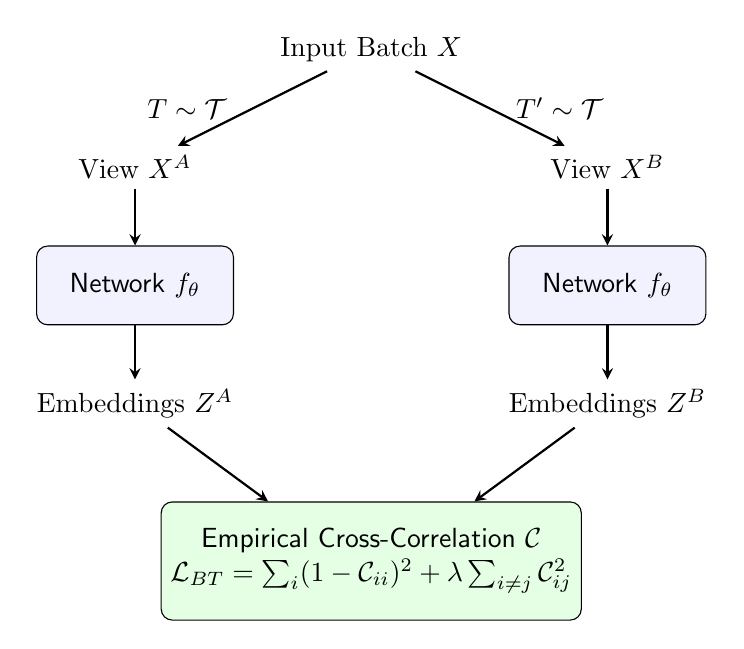
\begin{tikzpicture}[
    box/.style={draw, rectangle, minimum width=2.5cm, minimum height=1cm, fill=blue!5, font=\sffamily, rounded corners},
    arrow/.style={->, thick, >=stealth}
]
\node (x) at (0, 0) {Input Batch $X$};
\node (xa) at (-3, -1.5) {View $X^A$};
\node (xb) at (3, -1.5) {View $X^B$};
\node[box] (fa) at (-3, -3) {Network $f_\theta$};
\node[box] (fb) at (3, -3) {Network $f_\theta$};
\node (za) at (-3, -4.5) {Embeddings $Z^A$};
\node (zb) at (3, -4.5) {Embeddings $Z^B$};
\node[box, fill=green!10, minimum width=5cm, minimum height=1.5cm, align=center] (loss) at (0, -6.5) {Empirical Cross-Correlation $\mathcal{C}$ \\ $\mathcal{L}_{\text{BT}} = \sum_i (1-\mathcal{C}_{ii})^2 + \lambda \sum_{i \neq j} \mathcal{C}_{ij}^2$};

\draw[arrow] (x) -- (xa) node[midway, left=2mm] {$T \sim \mathcal{T}$};
\draw[arrow] (x) -- (xb) node[midway, right=2mm] {$T' \sim \mathcal{T}$};
\draw[arrow] (xa) -- (fa);
\draw[arrow] (xb) -- (fb);
\draw[arrow] (fa) -- (za);
\draw[arrow] (fb) -- (zb);
\draw[arrow] (za) -- (loss.150);
\draw[arrow] (zb) -- (loss.30);
\end{tikzpicture}
\caption{The Barlow Twins architecture. Instead of contrasting individual samples, the objective forces the cross-correlation matrix of the batch features to approximate the identity matrix.}
\label{fig:bt_arch}
\end{figure}

\section{Information-Theoretic Equivalence}

The intuitive mechanism of Barlow Twins maps formally to maximizing mutual information. Contrastive methods maximize $I(X^A; Z^B)$ using bounds like InfoNCE. Redundancy reduction methods achieve the same end by decomposing the mutual information.

\begin{theorem}[Barlow Twins and Information Maximization]
Assume that the embeddings $Z^A$ and $Z^B$ are jointly Gaussian vectors in $\mathbb{R}^d$. Minimizing the Barlow Twins loss $\mathcal{L}_{\text{BT}}$ serves as a surrogate for maximizing the mutual information $I(Z^A; Z^B)$ under the constraint of feature decorrelation.
\end{theorem}
\begin{proof}
Recall the mutual information can be written as:
\begin{equation}
    I(Z^A; Z^B) = H(Z^A) - H(Z^A | Z^B)
\end{equation}
For a $d$-dimensional multivariate Gaussian $Z \sim \mathcal{N}(\mu, \Sigma)$, the differential entropy is $h(Z) = \frac{1}{2} \log \det(2\pi e \Sigma)$.
To maximize $H(Z^A)$, we wish to maximize $\det(\Sigma^A)$. Because the Barlow Twins framework standardizes the variance of each feature (so the trace of $\Sigma^A$ is fixed to $d$), Hadamard's inequality states that $\det(\Sigma^A) \leq \prod_{i=1}^d \Sigma^A_{ii} = 1$, with equality occurring if and only if $\Sigma^A$ is a diagonal matrix.
Thus, by penalizing the off-diagonal elements of the cross-correlation matrix (and implicitly the auto-correlation matrix), the redundancy reduction term $\sum_{i \neq j} \mathcal{C}_{ij}^2$ pushes the covariance structure toward the identity matrix, effectively maximizing the marginal entropy $H(Z^A)$ and $H(Z^B)$ within the constrained space.

Conversely, the conditional entropy $H(Z^A | Z^B)$ measures the uncertainty in $Z^A$ given $Z^B$. By driving the diagonal elements $\mathcal{C}_{ii}$ to 1, the invariance term forces $Z^A$ to be perfectly predictable from $Z^B$ for each dimension, thereby minimizing $H(Z^A | Z^B)$.
Consequently, combining these terms maximizes $I(Z^A; Z^B)$ without necessitating negative samples.
\end{proof}

\begin{figure}[ht]
\centering
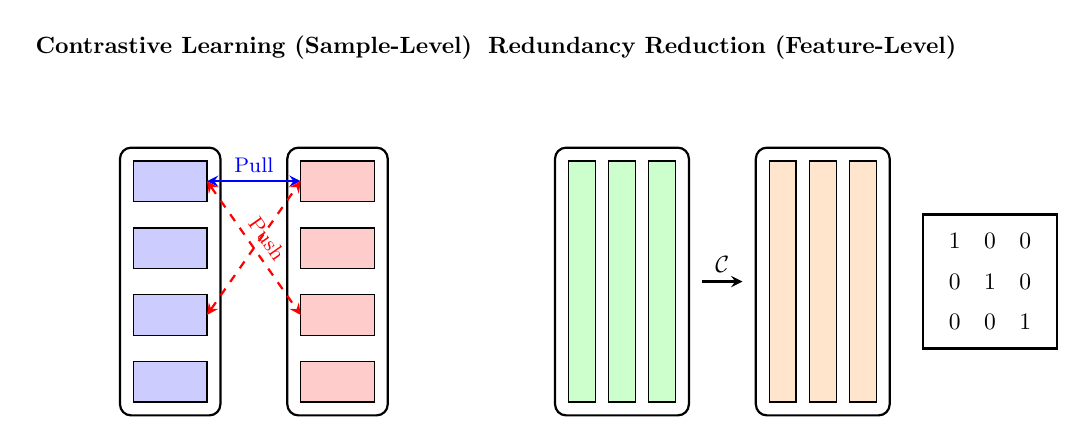
\begin{tikzpicture}[scale=0.85, transform shape, >=stealth]
% Contrastive
\node[align=center, font=\bfseries] at (2, 5.5) {Contrastive Learning   (Sample-Level)};
\draw[thick, rounded corners] (0, 0) rectangle (1.5, 4);
\draw[thick, rounded corners] (2.5, 0) rectangle (4, 4);
\foreach \y in {0.5, 1.5, 2.5, 3.5} {
    \draw[fill=blue!20] (0.2, \y-0.3) rectangle (1.3, \y+0.3);
    \draw[fill=red!20] (2.7, \y-0.3) rectangle (3.8, \y+0.3);
}
\draw[<->, thick, blue] (1.3, 3.5) -- (2.7, 3.5) node[midway, above] {\small Pull};
\draw[<->, thick, red, dashed] (1.3, 3.5) -- (2.7, 1.5) node[midway, sloped, above] {\small Push};
\draw[<->, thick, red, dashed] (1.3, 1.5) -- (2.7, 3.5);

% Redundancy Reduction
\node[align=center, font=\bfseries] at (9, 5.5) {Redundancy Reduction   (Feature-Level)};
\draw[thick, rounded corners] (6.5, 0) rectangle (8.5, 4);
\draw[thick, rounded corners] (9.5, 0) rectangle (11.5, 4);
\foreach \x in {6.7, 7.3, 7.9} {
    \draw[fill=green!20] (\x, 0.2) rectangle (\x+0.4, 3.8);
}
\foreach \x in {9.7, 10.3, 10.9} {
    \draw[fill=orange!20] (\x, 0.2) rectangle (\x+0.4, 3.8);
}
\draw[->, thick] (8.7, 2) -- (9.3, 2) node[midway, above] {$\mathcal{C}$};

\draw[thick] (12, 1) rectangle (14, 3);
\node at (13, 2.6) {$1 \quad 0 \quad 0$};
\node at (13, 2.0) {$0 \quad 1 \quad 0$};
\node at (13, 1.4) {$0 \quad 0 \quad 1$};
\end{tikzpicture}
\caption{Comparison of representation learning paradigms. Left: Contrastive learning relies on sample-to-sample interactions, pulling positives and pushing negatives. Right: Redundancy reduction computes correlations across feature columns over the entire batch, driving the cross-correlation matrix to the identity.}
\label{fig:paradigm_compare}
\end{figure}

\section{Numerical Example: Matrix Computation}
To demystify the mechanics, let us compute the Barlow Twins loss for a toy batch of size $B=2$ and dimensionality $d=2$. Let the unnormalized embeddings for view $A$ and view $B$ be:
\begin{equation}
    U^A = \begin{bmatrix} 2 & 4 \\ -2 & 0 \end{bmatrix}, \quad U^B = \begin{bmatrix} 3 & -1 \\ -1 & 3 \end{bmatrix}
\end{equation}
where rows are batch instances and columns are features. 
First, we mean-center and standardize each column (with $\epsilon = 0$). 
For $U^A$:
Column 1 has mean $0$ and variance $\frac{(2)^2 + (-2)^2}{2} = 4$, standard deviation $2$.
Column 2 has mean $2$ and variance $\frac{(4-2)^2 + (0-2)^2}{2} = 4$, standard deviation $2$.
Normalizing yields $Z^A$:
\begin{equation}
    Z^A = \begin{bmatrix} 1 & 1 \\ -1 & -1 \end{bmatrix}
\end{equation}
For $U^B$:
Column 1 has mean $1$, standard deviation $2$. Centering yields $[2, -2]^\top$; normalizing yields $[1, -1]^\top$.
Column 2 has mean $1$, standard deviation $2$. Centering yields $[-2, 2]^\top$; normalizing yields $[-1, 1]^\top$.
\begin{equation}
    Z^B = \begin{bmatrix} 1 & -1 \\ -1 & 1 \end{bmatrix}
\end{equation}
The cross-correlation matrix is $\mathcal{C} = \frac{1}{B} (Z^A)^\top Z^B$:
\begin{equation}
    \mathcal{C} = \frac{1}{2} \begin{bmatrix} 1 & -1 \\ 1 & -1 \end{bmatrix} \begin{bmatrix} 1 & -1 \\ -1 & 1 \end{bmatrix} = \frac{1}{2} \begin{bmatrix} (1+1) & (-1-1) \\ (1+1) & (-1-1) \end{bmatrix} = \begin{bmatrix} 1 & -1 \\ 1 & -1 \end{bmatrix}
\end{equation}
The diagonal elements are $\mathcal{C}_{11} = 1$ and $\mathcal{C}_{22} = -1$. The off-diagonal elements are $\mathcal{C}_{12} = -1$ and $\mathcal{C}_{21} = 1$.
Assuming $\lambda = 1$, the loss evaluates to:
\begin{equation}
    \mathcal{L}_{\text{BT}} = (1 - 1)^2 + (1 - (-1))^2 + (-1)^2 + (1)^2 = 0 + 4 + 1 + 1 = 6
\end{equation}
The non-zero loss stems entirely from $\mathcal{C}_{22} = -1$ (view B's second feature is perfectly anti-correlated with view A's second feature) and the strong cross-feature correlations. Gradient descent will adjust network weights to rotate the embeddings until $\mathcal{C} \approx I$, minimizing the loss to 0.

\section{VICReg: Variance, Invariance, and Covariance}
While Barlow Twins integrates normalization into the correlation calculation, VICReg (Variance-Invariance-Covariance Regularization) explicitly separates these constraints into distinct terms. This provides finer control over the representation structure.

For embeddings $Z^A, Z^B$ (without batch normalization applied), VICReg defines three objectives:

1. \textbf{Invariance}: The mean squared distance between representations of the same image:
\begin{equation}
    s(Z^A, Z^B) = \frac{1}{B} \sum_{b=1}^B \|z^A_b - z^B_b\|_2^2
\end{equation}

2. \textbf{Variance}: A hinge loss ensuring the variance of each feature exceeds a threshold $\gamma$ (preventing point collapse):
\begin{equation}
    v(Z) = \frac{1}{d} \sum_{i=1}^d \max(0, \gamma - \sqrt{\text{Var}(Z_{\cdot, i}) + \epsilon})
\end{equation}

3. \textbf{Covariance}: A penalty on the off-diagonal elements of the covariance matrix, forcing features to be linearly independent (preventing dimensional collapse):
\begin{equation}
    c(Z) = \frac{1}{d} \sum_{i \neq j} [\text{Cov}(Z)]_{i,j}^2
\end{equation}

The total VICReg loss is the weighted sum:
\begin{equation}
    \mathcal{L}_{\text{VICReg}} = \lambda s(Z^A, Z^B) + \mu \big(v(Z^A) + v(Z^B)\big) + \nu \big(c(Z^A) + c(Z^B)\big)
\end{equation}

\begin{lemma}[Avoidance of Collapse in VICReg]
Let $\mathcal{L}_{\text{VICReg}}$ achieve its global minimum. For any $\gamma > 0$ and $\mu > 0$, the learned representation cannot trivially collapse to a constant vector $z_c$.
\end{lemma}
\begin{proof}
Assume, for contradiction, that the network collapses representations such that for all $b$, $z^A_b = z^B_b = z_c$ for some constant $z_c \in \mathbb{R}^d$. 
The invariance term becomes $s(Z^A, Z^B) = 0$. 
The covariance term becomes $c(Z^A) = c(Z^B) = 0$, as the variables are constant. 
However, for a constant vector, the empirical variance across the batch is $\text{Var}(Z_{\cdot, i}) = 0$.
The variance term thus evaluates to $v(Z) = \frac{1}{d} \sum_{i=1}^d \max(0, \gamma - 0) = \gamma$.
The total loss is $2\mu\gamma$.
If the network instead maps the batch to vectors distributed on a sphere of radius $\sqrt{d}\gamma$ such that they are uncorrelated and mean-centered, the variance term becomes $0$, the covariance term becomes $0$, and if $Z^A = Z^B$, the invariance term is $0$. This non-collapsed configuration achieves a loss of $0 < 2\mu\gamma$. Therefore, a trivial collapse cannot be the global minimum.
\end{proof}

% 3. Horizon Box
\begin{horizon}
While Barlow Twins and VICReg mathematically preclude exact representation collapse, they introduce deep theoretical mysteries regarding the optimal dimensionality of the latent space. 

It is conjectured that the optimal choice of the trade-off hyperparameters ($\lambda$ in Barlow Twins, or the ratio $\nu/\mu$ in VICReg) is strictly bounded by the intrinsic dimensionality of the underlying data manifold. If the weighting of the redundancy reduction term is set too high on a dataset with low intrinsic rank, the network is forced to "invent" uncorrelated noise just to satisfy the full-rank covariance objective. 

An open question is whether non-contrastive redundancy reduction objectives are secretly equivalent to specific constrained continuous-time diffusion processes. Future work might show that the process of expanding the covariance matrix to the identity while maintaining pairwise invariance forms an exact duality with the reverse-time Langevin dynamics of a denoiser, unifying contrastive self-supervised learning with modern generative diffusion.
\end{horizon}

% 4. Summary + Exercises
\section{Summary}
In this chapter, we investigated how to avoid representation collapse without the burdensome reliance on negative sampling. By shifting the computational perspective from the sample dimension to the feature dimension, redundancy reduction enforces that the covariance or cross-correlation matrix of the embeddings approaches the identity matrix. We proved that this mechanism acts as a tractable bound on maximizing mutual information. The Barlow Twins architecture integrates this directly into a unified correlation loss, while VICReg explicitly partitions the geometry of the representation space into distinct variance, invariance, and covariance penalties.

\section{Exercises}
\begin{enumerate}
    \item \textbf{Feature Orthogonality:} Prove that if the empirical cross-correlation matrix $\mathcal{C}$ perfectly reaches the identity matrix $I_d$, and $Z^A = Z^B$, then the columns of the representation matrix $Z^A$ are strictly orthogonal. 
    \item \textbf{Gradients of the Barlow Twins Loss:} Compute the partial derivative of $\mathcal{L}_{\text{BT}}$ with respect to a single normalized feature embedding $\tilde{z}^A_{b,i}$. How does the gradient encourage anti-correlation when $\mathcal{C}_{i,j} > 0$?
    \item \textbf{Role of the Variance Hinge:} In the VICReg loss, consider replacing the variance term $v(Z)$ with a standard mean squared error target to a fixed scalar variance, $v'(Z) = \frac{1}{d} \sum_{i=1}^d (\gamma - \text{Var}(Z_i))^2$. Analyze how this modification affects the flexibility of the learned representations compared to the hinge loss $\max(0, \gamma - \sqrt{\text{Var}(Z_i)})$. Does it overly constrain the geometry?
\end{enumerate}

% TODO-CITE: Ensure all named results are cited.

\chapter{Cross-Modal Mutual Information: CLIP and Alignment}

\section{Introduction: The Babel of Modalities}

In human cognition, information is rarely unimodal. Our understanding of the world is formed through a continuous, integrated stream of visual, auditory, and textual stimuli. When we encounter a dog, we see its shape, hear its bark, and attach the linguistic label ``dog'' to the entire sensory package. In the context of deep learning, these distinct channels of information—referred to as modalities—have historically been treated in isolation. Convolutional networks were designed to process grids of pixels, while transformers were tuned for sequences of discrete tokens. The representations learned by these architectures resided in disjoint geometric spaces; the vector representing the image of a dog bore no mathematical relationship to the vector representing the string of text ``a picture of a dog.''

The phenomenon of cross-modal alignment is the attempt to bridge this divide. By projecting different modalities into a shared latent space, models can establish a common semantic language. The breakthrough in this domain was catalyzed by Contrastive Language-Image Pretraining (CLIP), which demonstrated that vast quantities of loosely correlated image-text pairs could be leveraged to learn a highly robust, unified representation space. 

At its core, cross-modal alignment is an information-theoretic optimization problem. We are given two views of a shared underlying concept. The image and the text are both noisy, high-dimensional projections of an abstract semantic idea. Our goal is to extract the information that is common to both modalities while discarding the modality-specific noise—the exact pixel arrangement or the idiosyncratic choice of syntax. In other words, we seek representations that maximize the mutual information between the two modalities. 

However, explicitly computing the mutual information between high-dimensional continuous random variables is computationally intractable. Instead, modern alignment models rely on variational bounds. By formulating the learning objective as a contrastive task—discriminating matched image-text pairs from mismatched ones—we implicitly optimize a lower bound on the true mutual information. This chapter formalizes the cross-modal alignment process, rigorously linking the mechanics of dual-encoder architectures and the InfoNCE loss to the maximization of mutual information.

\section{The Cross-Modal InfoNCE Bound}

Let $X_1 \in \mathcal{X}_1$ represent data from the first modality (e.g., images) and $X_2 \in \mathcal{X}_2$ represent data from the second modality (e.g., text). We assume that paired observations $(x_1, x_2)$ are drawn from an unknown joint distribution $P_{X_1, X_2}$. The marginal distributions are $P_{X_1}$ and $P_{X_2}$.

We introduce two deep neural networks acting as encoders: $f_{\theta_1} : \mathcal{X}_1 \to \mathcal{Z}_1$ and $f_{\theta_2} : \mathcal{X}_2 \to \mathcal{Z}_2$, which map the input data to continuous latent representations $Z_1$ and $Z_2$. 

\begin{figure}[ht]
    \centering
    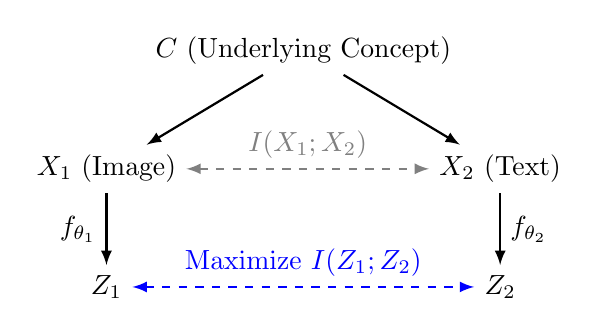
\begin{tikzpicture}[node distance=2.5cm, auto, thick, >=latex]
        % Nodes
        \node (C) at (2.5, 3) {$C$ (Underlying Concept)};
        \node (X1) at (0, 1.5) {$X_1$ (Image)};
        \node (Z1) at (0, 0) {$Z_1$};
        \node (X2) at (5, 1.5) {$X_2$ (Text)};
        \node (Z2) at (5, 0) {$Z_2$};
        
        % Arrows
        \draw[->] (C) -- (X1);
        \draw[->] (C) -- (X2);
        \draw[->] (X1) -- node[left] {$f_{\theta_1}$} (Z1);
        \draw[->] (X2) -- node[right] {$f_{\theta_2}$} (Z2);
        
        % Mutual Info Links
        \draw[<->, dashed, blue] (Z1) -- node[above] {Maximize $I(Z_1; Z_2)$} (Z2);
        \draw[<->, dashed, gray] (X1) -- node[above] {$I(X_1; X_2)$} (X2);
    \end{tikzpicture}
    \caption{The Markov structure of cross-modal alignment. The data processing inequality guarantees that $I(Z_1; Z_2) \le I(X_1; X_2)$. The objective of the encoders $f_{\theta_1}$ and $f_{\theta_2}$ is to preserve as much of the shared information derived from the true concept $C$ as possible.}
    \label{fig:clip_markov}
\end{figure}

By the Data Processing Inequality (DPI) applied to the Markov chain $Z_1 \leftarrow X_1 \leftrightarrow X_2 \rightarrow Z_2$, the mutual information between the representations is bounded by the mutual information between the raw modalities:
\begin{equation}
    I(Z_1; Z_2) \le I(X_1; X_2)
\end{equation}
Our objective is to find parameters $\theta_1, \theta_2$ that maximize $I(Z_1; Z_2)$. We approach this via contrastive estimation. Given a batch of $N$ pairs $\{(x_{1,i}, x_{2,i})\}_{i=1}^N$ drawn independent and identically distributed (i.i.d.) from $P_{X_1, X_2}$, we define a similarity scoring function (critic) $s(z_1, z_2) \in \mathbb{R}$. In CLIP, this is typically the scaled cosine similarity $s(z_1, z_2) = \frac{z_1^\top z_2}{\tau}$, where $\tau > 0$ is a temperature parameter.

The contrastive loss for predicting the correct text representation given an image representation is defined as:
\begin{equation}
    \mathcal{L}_{1 \to 2} = - \frac{1}{N} \sum_{i=1}^N \log \frac{\exp(s(z_{1,i}, z_{2,i}))}{\sum_{j=1}^N \exp(s(z_{1,i}, z_{2,j}))}
\end{equation}
This loss treats the matching text $z_{2,i}$ as the positive sample and the remaining $N-1$ texts $z_{2,j}$ in the batch as negative samples drawn from the marginal distribution $P_{Z_2}$.

\begin{theorem}[Cross-Modal InfoNCE Bound]
Let the negative samples in the denominator of $\mathcal{L}_{1 \to 2}$ be drawn i.i.d. from the marginal distribution $P_{Z_2}$. For any scoring function $s(z_1, z_2)$, the expected contrastive loss bounds the mutual information between the latent representations:
\begin{equation}
    I(Z_1; Z_2) \ge \log N - \mathbb{E}\left[\mathcal{L}_{1 \to 2}\right]
\end{equation}
\end{theorem}

\begin{proof}
Consider the optimal choice for the critic function $s^*(z_1, z_2)$. In a classification task where one seeks to identify the positive pair among $N$ choices (one positive drawn from the joint $P_{Z_1, Z_2}$ and $N-1$ negatives drawn from the product of marginals $P_{Z_1}P_{Z_2}$), the optimal classifier models the posterior probability of a sample coming from the joint distribution. 

By Bayes' theorem, the probability that the $i$-th sample is the positive pair, given the set of candidate pairs $S_i = \{ (z_{1,i}, z_{2,j}) \}_{j=1}^N$, is exactly:
\begin{equation}
    p(C=i | S_i) = \frac{\frac{p(z_{1,i}, z_{2,i})}{p(z_{1,i})p(z_{2,i})}}{\sum_{j=1}^N \frac{p(z_{1,i}, z_{2,j})}{p(z_{1,i})p(z_{2,j})}}
\end{equation}
This implies the optimal score function is proportional to the log density ratio: $s^*(z_1, z_2) = \log \frac{p(z_1, z_2)}{p(z_1)p(z_2)} + \text{const}$.

Substituting the optimal critic into the expected loss:
\begin{align*}
    \mathbb{E}\left[\mathcal{L}_{1 \to 2}\right] &= \mathbb{E}_{S} \left[ - \log \frac{\frac{p(z_1, z_2)}{p(z_1)p(z_2)}}{\frac{p(z_1, z_2)}{p(z_1)p(z_2)} + \sum_{j \neq i} \frac{p(z_1, z_{2,j})}{p(z_1)p(z_{2,j})}} \right] \\
    &= \mathbb{E}_{S} \left[ \log \left( 1 + \frac{p(z_1)p(z_2)}{p(z_1, z_2)} \sum_{j \neq i} \frac{p(z_1, z_{2,j})}{p(z_1)p(z_{2,j})} \right) \right]
\end{align*}
By Jensen's inequality applied to the concave $\log$ function, we can move the expectation inside for the terms involving the negative samples:
\begin{align*}
    \mathbb{E}\left[\mathcal{L}_{1 \to 2}\right] &\ge \mathbb{E}_{(Z_1,Z_2)\sim P_{Z_1, Z_2}} \left[ \log \left( 1 + \frac{p(z_1)p(z_2)}{p(z_1, z_2)} (N-1) \mathbb{E}_{z_{2}' \sim P_{Z_2}} \left[ \frac{p(z_1, z_{2}')}{p(z_1)p(z_{2}')} \right] \right) \right]
\end{align*}
Since $\mathbb{E}_{z_{2}' \sim P_{Z_2}} \left[ \frac{p(z_1, z_{2}')}{p(z_1)p(z_{2}')} \right] = \int p(z_{2}') \frac{p(z_1|z_{2}')}{p(z_1)} dz_{2}' = \frac{p(z_1)}{p(z_1)} = 1$, we have:
\begin{align*}
    \mathbb{E}\left[\mathcal{L}_{1 \to 2}\right] &\ge \mathbb{E}_{P_{Z_1, Z_2}} \left[ \log \left( 1 + \frac{p(z_1)p(z_2)}{p(z_1, z_2)} (N-1) \right) \right] \\
    &\approx \mathbb{E}_{P_{Z_1, Z_2}} \left[ \log \left( N \frac{p(z_1)p(z_2)}{p(z_1, z_2)} \right) \right] \quad \text{for large } N \\
    &= \log N - \mathbb{E}_{P_{Z_1, Z_2}} \left[ \log \frac{p(z_1, z_2)}{p(z_1)p(z_2)} \right] \\
    &= \log N - I(Z_1; Z_2)
\end{align*}
Rearranging terms yields $I(Z_1; Z_2) \ge \log N - \mathbb{E}\left[\mathcal{L}_{1 \to 2}\right]$.
\end{proof}

\section{Symmetry and Dual-Encoder Dynamics}

The bound derived above considers the prediction of text from images. By symmetry, the task of predicting an image from text yields the conjugate loss:
\begin{equation}
    \mathcal{L}_{2 \to 1} = - \frac{1}{N} \sum_{i=1}^N \log \frac{\exp(s(z_{1,i}, z_{2,i}))}{\sum_{k=1}^N \exp(s(z_{1,k}, z_{2,i}))}
\end{equation}
While $\mathcal{L}_{1 \to 2}$ normalizes over the text embeddings in the batch, $\mathcal{L}_{2 \to 1}$ normalizes over the image embeddings. In practice, the distributions of image embeddings and text embeddings can have different geometries and varying degrees of mode collapse. To ensure a balanced optimization that penalizes "hub" vectors in both modality spaces, the complete CLIP objective averages both directions:
\begin{equation}
    \mathcal{L}_{\text{CLIP}} = \frac{1}{2} \left( \mathcal{L}_{1 \to 2} + \mathcal{L}_{2 \to 1} \right)
\end{equation}

\begin{figure}[ht]
    \centering
    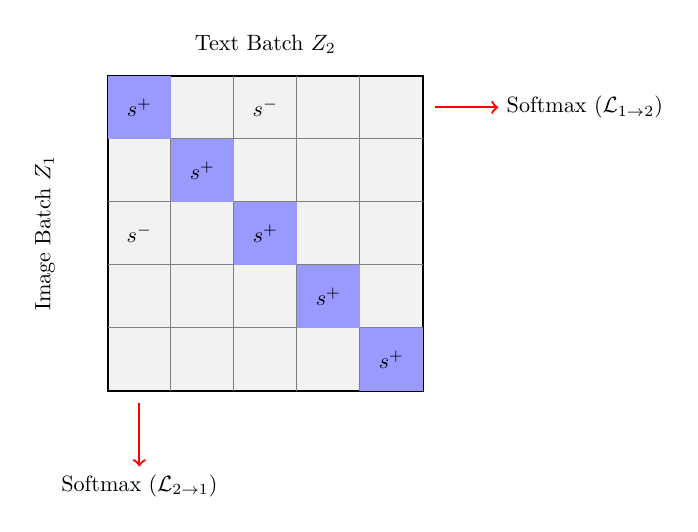
\begin{tikzpicture}[scale=0.8, transform shape]
        % Draw matrix
        \draw[thick, fill=gray!10] (0,0) rectangle (5,5);
        \foreach \i in {1,2,3,4} {
            \draw[gray] (0,\i) -- (5,\i);
            \draw[gray] (\i,0) -- (\i,5);
        }
        % Diagonal
        \foreach \i in {0,1,2,3,4} {
            \fill[blue!40] (\i, 4-\i) rectangle (\i+1, 5-\i);
            \node at (\i+0.5, 4.5-\i) {$s^+$};
        }
        
        % Off-diagonals (example)
        \node at (2.5, 4.5) {$s^-$};
        \node at (0.5, 2.5) {$s^-$};

        % Text nodes
        \node[rotate=90] at (-1, 2.5) {Image Batch $Z_1$};
        \node at (2.5, 5.5) {Text Batch $Z_2$};
        
        % Braces and labels
        \draw[thick, ->, red] (5.2, 4.5) -- (6.2, 4.5) node[right, black] {Softmax ($\mathcal{L}_{1 \to 2}$)};
        \draw[thick, ->, red] (0.5, -0.2) -- (0.5, -1.2) node[below, black] {Softmax ($\mathcal{L}_{2 \to 1}$)};
        
    \end{tikzpicture}
    \caption{The pairwise similarity matrix computed during a forward pass of CLIP. The objective maximizes the similarities on the diagonal (positive pairs $s^+$) while minimizing the off-diagonal elements (negative pairs $s^-$). The symmetric loss computes softmax cross-entropies across both rows and columns.}
    \label{fig:clip_matrix}
\end{figure}

This dual maximization restricts the encoders from ignoring the statistical structures of either domain. The true mutual information is symmetric, $I(Z_1; Z_2) = I(Z_2; Z_1)$, and both losses operate as strict lower bounds on the same underlying quantity. By optimizing their average, the training dynamics become more stable, mitigating gradients that might aggressively push one modality into a degenerate state.

\section{A Numerical Example: The Batch Size Bottleneck}

To build intuition for the bound $I(Z_1; Z_2) \ge \log N - \mathcal{L}$, consider a stylized numerical example. Suppose the shared semantic concept $C$ is a standard normal scalar $C \sim \mathcal{N}(0, 1)$. The modalities are noisy projections of this concept:
\begin{align*}
    X_1 &= C + \epsilon_1 \\
    X_2 &= C + \epsilon_2
\end{align*}
where $\epsilon_1, \epsilon_2 \sim \mathcal{N}(0, \sigma^2)$ are independent Gaussian noise. 
The joint distribution of $(X_1, X_2)$ is bivariate Gaussian with mean zero and covariance matrix:
\begin{equation}
    \Sigma = \begin{pmatrix} 1 + \sigma^2 & 1 \\ 1 & 1 + \sigma^2 \end{pmatrix}
\end{equation}
The true mutual information can be calculated precisely using differential entropy:
\begin{align*}
    I(X_1; X_2) &= h(X_1) + h(X_2) - h(X_1, X_2) \\
    &= \frac{1}{2} \log (2\pi e (1+\sigma^2)) + \frac{1}{2} \log (2\pi e (1+\sigma^2)) - \frac{1}{2} \log ( (2\pi e)^2 |\Sigma| ) \\
    &= \frac{1}{2} \log \left( \frac{(1+\sigma^2)^2}{(1+\sigma^2)^2 - 1} \right) = \frac{1}{2} \log \left( 1 + \frac{1}{2\sigma^2 + \sigma^4} \right)
\end{align*}

Observe what happens as the noise $\sigma \to 0$: the mutual information $I(X_1; X_2)$ diverges to infinity, meaning the variables perfectly determine each other. However, our InfoNCE bound is rigorously capped:
\begin{equation}
    \log N - \mathcal{L}_{1 \to 2} \le \log N
\end{equation}
Because the cross-entropy loss $\mathcal{L}_{1 \to 2}$ is non-negative, the tightest our bound can ever become is $\log N$. 
If we use a batch size of $N=256$, the maximum mutual information the loss function can ever ``see'' is $\log(256) \approx 5.54$ nats. If the true mutual information between an image and its caption requires $10$ nats to capture all granular semantic details (colors, object counts, backgrounds), a batch size of $256$ is mathematically incapable of providing gradients that encourage the encoders to capture those finer details once $5.54$ nats of information are already shared. The critic saturates.

This simple numerical artifact explains a core engineering reality of modern cross-modal models: they require exorbitant batch sizes. CLIP was trained with a batch size of $N=32,768$ (yielding a maximum bound of $\approx 10.4$ nats) specifically to raise the ceiling on the mutual information estimator, forcing the model to align on subtle, intricate semantics rather than just obvious, surface-level features.

\begin{horizon}
The mathematical necessity of massive batch sizes in contrastive learning highlights a fundamental vulnerability: the strict reliance on negative samples to formulate a partition function. It is conjectured that future multimodal architectures will entirely abandon InfoNCE in favor of non-contrastive redundancy-reduction criteria, such as those seen in Barlow Twins, scaling them across continuous multimodal domains.

A significant open question remains regarding the nature of the ``shared subspace'' $I(Z_1; Z_2)$. While current models successfully map nouns to objects, it is suspected that this intersection captures only a superficial projection of semantics. Does the geometry of the text latent space truly warp to adopt the spatial symmetries of the image space? Or does the model simply hash co-occurring patterns into arbitrary but matching clusters? 

Future work might show that simply maximizing $I(Z_1; Z_2)$ is insufficient for true multimodal reasoning. We may require structural constraints—perhaps mapping text not to points, but to functional transformations that operate on the image manifold—to graduate from mere alignment to compositional multimodal understanding.
\end{horizon}

\section{Summary}
In this chapter, we explored the information-theoretic foundations of cross-modal alignment, focusing on the CLIP architecture. We demonstrated that aligning image and text vectors via a contrastive loss is equivalent to maximizing a variational lower bound on their mutual information. Through the InfoNCE derivation, we established that the bound is strictly capped by $\log N$, dictating the necessity of massive batch sizes in practice. Furthermore, the symmetric loss formulation ensures stable representation learning by balancing the negative sampling over both marginal distributions.

\section{Exercises}
\begin{enumerate}
    \item \textbf{Temperature Scaling:} In CLIP, the similarity function is scaled by a learned temperature $\tau$, such that $s(z_1, z_2) = \frac{z_1^\top z_2}{\tau}$. Prove that if the embeddings $Z_1, Z_2$ are unconstrained (i.e., not normalized to the unit hypersphere), the temperature parameter $\tau$ is mathematically redundant and can be absorbed into the weights of the encoders. 
    \item \textbf{Biased Negatives:} The derivation of the InfoNCE bound assumes that negative samples are drawn i.i.d. from the true marginal distribution $P_{Z_2}$. Suppose instead that the batch is constructed using ``hard negatives''—samples drawn from a biased distribution $Q_{Z_2}$ that overweights items similar to $Z_1$. Derive the modified lower bound on $I(Z_1; Z_2)$ under this sampling strategy. How does the penalty term relate to the Kullback-Leibler divergence $D_{\text{KL}}(Q_{Z_2} \parallel P_{Z_2})$?
    \item \textbf{Multimodal Saturation:} Extend the bivariate Gaussian example. Suppose there are three modalities $X_1, X_2, X_3$ all generated from $C \sim \mathcal{N}(0,1)$ with independent noise variance $\sigma^2$. If we optimize pairwise CLIP losses between all three pairs, what is the theoretical maximum mutual information $I(Z_1; Z_2; Z_3)$ that can be bounded, assuming a batch size of $N$ across all modalities?
\end{enumerate}

% TODO-CITE: Ensure all named results are cited.


\part{Divergences and Adversarial Networks}
\chapter{Integral Probability Metrics}
\label{ch:ipm}

\section{Distances Between Distributions: Beyond Pointwise Comparison}

In the study of deep learning and information theory, we frequently encounter the need to measure the discrepancy between two probability distributions. Whether we are training a generative model to match a data distribution, or bounding the generalization gap of a learned representation, the choice of divergence is paramount. Up to this point, our primary tools have been the Kullback-Leibler (KL) divergence and its generalizations, the $f$-divergences. While structurally beautiful and deeply connected to Shannon entropy, $f$-divergences suffer from a fatal flaw in the context of modern machine learning: they require the distributions to have overlapping support. 

When $P$ and $Q$ have disjoint supports, as is often the case when data lies on a low-dimensional manifold embedded in a high-dimensional space (the Manifold Hypothesis, Chapter 5), the KL divergence $D_{\text{KL}}(P \parallel Q)$ explodes to infinity or becomes undefined. It provides no useful gradient signal for optimization. A model generating perfectly realistic images that are shifted by a single pixel might be penalized infinitely, simply because the exact point in the pixel space has zero probability under the true distribution.

To overcome this, we must shift our perspective from \textit{pointwise ratios of densities} to \textit{expectations of functions}. Instead of asking how much the densities $p(x)$ and $q(x)$ differ at each point $x$, we can ask: what is the maximum discrepancy in the expected value of a function drawn from a specific class when the data is drawn from $P$ versus $Q$? If we can find a function (a "critic" or "discriminator") that yields a very different average value on $P$ than on $Q$, then the distributions must be far apart. If no such function can tell them apart, the distributions are close.

This is the foundational intuition behind \textit{Integral Probability Metrics} (IPMs). By selecting different classes of functions---such as bounded functions, Lipschitz-continuous functions, or functions in a Reproducing Kernel Hilbert Space (RKHS)---we recover a rich family of metrics. Because IPMs integrate over the distributions, they naturally "smooth out" local singularities and provide meaningful, continuous distance measures even when distributions are mutually singular. This paradigm shift paves the way for advanced generative modeling, most notably the Wasserstein GAN, and provides robust statistical tests for two-sample problems.

\section{The Mathematical Formulation of IPMs}

We begin by formally defining an Integral Probability Metric. Let $P$ and $Q$ be probability measures defined on a measurable space $\mathcal{X}$. Let $\mathcal{F}$ be a class of real-valued bounded measurable functions $f: \mathcal{X} \to \mathbb{R}$.

\begin{definition}[Integral Probability Metric]
The Integral Probability Metric (IPM) between distributions $P$ and $Q$ with respect to the function class $\mathcal{F}$ is defined as:
\begin{equation}
    \gamma_{\mathcal{F}}(P, Q) = \sup_{f \in \mathcal{F}} \left| \mathbb{E}_{X \sim P}[f(X)] - \mathbb{E}_{Y \sim Q}[f(Y)] \right|.
\end{equation}
\end{definition}

In practice, we almost always choose a function class $\mathcal{F}$ that is \textit{symmetric}, meaning if $f \in \mathcal{F}$, then $-f \in \mathcal{F}$. This greatly simplifies the definition.

\begin{theorem}[Symmetric IPMs]
\label{thm:ipm_symmetric}
If the function class $\mathcal{F}$ is symmetric (i.e., $f \in \mathcal{F} \implies -f \in \mathcal{F}$), the absolute value in the IPM definition can be dropped:
\begin{equation}
    \gamma_{\mathcal{F}}(P, Q) = \sup_{f \in \mathcal{F}} \left( \mathbb{E}_{X \sim P}[f(X)] - \mathbb{E}_{Y \sim Q}[f(Y)] \right).
\end{equation}
\end{theorem}

\begin{proof}
Let $S = \sup_{f \in \mathcal{F}} \left| \mathbb{E}_{P}[f(X)] - \mathbb{E}_{Q}[f(Y)] \right|$. We want to show $S = S'$, where $S' = \sup_{f \in \mathcal{F}} ( \mathbb{E}_{P}[f(X)] - \mathbb{E}_{Q}[f(Y)] )$. 

First, for any $a \in \mathbb{R}$, $a \le |a|$, thus for any $f \in \mathcal{F}$:
\begin{equation*}
    \mathbb{E}_{P}[f(X)] - \mathbb{E}_{Q}[f(Y)] \le \left| \mathbb{E}_{P}[f(X)] - \mathbb{E}_{Q}[f(Y)] \right| \le S.
\end{equation*}
Taking the supremum over all $f \in \mathcal{F}$ yields $S' \le S$.

Second, by definition of the absolute value, for any $f$, $\left| \mathbb{E}_{P}[f(X)] - \mathbb{E}_{Q}[f(Y)] \right|$ is either $\mathbb{E}_{P}[f(X)] - \mathbb{E}_{Q}[f(Y)]$ or $-(\mathbb{E}_{P}[f(X)] - \mathbb{E}_{Q}[f(Y)])$. By linearity of expectation, the latter is equal to $\mathbb{E}_{P}[-f(X)] - \mathbb{E}_{Q}[-f(Y)]$.
Since $\mathcal{F}$ is symmetric, if $f \in \mathcal{F}$, then $-f \in \mathcal{F}$. Therefore, for every $f \in \mathcal{F}$, there exists $g \in \{f, -f\} \subseteq \mathcal{F}$ such that:
\begin{equation*}
    \left| \mathbb{E}_{P}[f(X)] - \mathbb{E}_{Q}[f(Y)] \right| = \mathbb{E}_{P}[g(X)] - \mathbb{E}_{Q}[g(Y)] \le S'.
\end{equation*}
Taking the supremum over $f \in \mathcal{F}$ gives $S \le S'$. Combining $S' \le S$ and $S \le S'$ proves that $S = S'$.
\end{proof}

\subsection{Specific Choices of Function Classes}

By instantiating $\mathcal{F}$ differently, we recover several celebrated distances in probability theory.

\subsubsection{Total Variation Distance}
Let $\mathcal{F}_{\text{TV}} = \{ f : \mathcal{X} \to \mathbb{R} \mid \sup_{x \in \mathcal{X}} |f(x)| \le 1 \}$. The resulting IPM is (up to a factor of 2) the Total Variation (TV) distance. This is the largest possible class of bounded functions, making TV distance very strong. If $P$ and $Q$ have disjoint supports, the supremum is achieved by setting $f(x)=1$ on the support of $P$ and $f(x)=-1$ on the support of $Q$, resulting in a distance of 2 (or 1 depending on normalization), failing to provide a gradient for continuous transformation.

\subsubsection{Wasserstein-1 Distance}
Let $\mathcal{X}$ be a metric space with distance metric $d(x, y)$. We choose $\mathcal{F}_{W}$ to be the set of all $1$-Lipschitz functions:
\begin{equation}
    \mathcal{F}_{W} = \{ f : \mathcal{X} \to \mathbb{R} \mid \forall x, y \in \mathcal{X}, |f(x) - f(y)| \le d(x, y) \}.
\end{equation}
By the Kantorovich-Rubinstein duality theorem, the resulting IPM is exactly the Wasserstein-1 distance (also known as the Earth Mover's Distance). 
The Lipschitz constraint enforces smoothness: $f(x)$ cannot jump abruptly. This provides continuous gradients even when distributions have disjoint supports, a property leveraged spectacularly in Wasserstein GANs.

\begin{figure}[htbp]
\centering
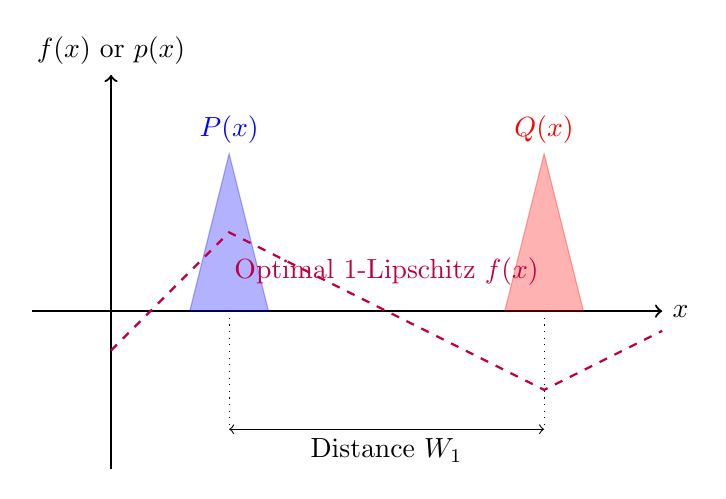
\begin{tikzpicture}
    % Axes
    \draw[->, thick] (-1, 0) -- (7, 0) node[right] {$x$};
    \draw[->, thick] (0, -2) -- (0, 3) node[above] {$f(x)$ or $p(x)$};
    
    % Distributions
    \filldraw[blue, opacity=0.3] (1,0) -- (1.5, 2) -- (2,0) -- cycle;
    \node[blue] at (1.5, 2.3) {$P(x)$};
    
    \filldraw[red, opacity=0.3] (5,0) -- (5.5, 2) -- (6,0) -- cycle;
    \node[red] at (5.5, 2.3) {$Q(x)$};
    
    % Lipschitz Function
    \draw[thick, dashed, purple] (0, -0.5) -- (1.5, 1) -- (5.5, -1) -- (7, -0.25);
    \node[purple] at (3.5, 0.5) {Optimal 1-Lipschitz $f(x)$};
    
    % Annotations
    \draw[<->] (1.5, -1.5) -- (5.5, -1.5) node[midway, below] {Distance $W_1$};
    \draw[dotted] (1.5, 0) -- (1.5, -1.5);
    \draw[dotted] (5.5, 0) -- (5.5, -1.5);
\end{tikzpicture}
\caption{The Wasserstein distance finds a smooth 1-Lipschitz function $f$ that maximizes the difference in expectations between $P$ and $Q$. The slope is bounded, ensuring that as $P$ translates towards $Q$, the distance changes continuously.}
\label{fig:wasserstein_ipm}
\end{figure}

\subsubsection{Maximum Mean Discrepancy (MMD)}
Let $\mathcal{H}$ be a Reproducing Kernel Hilbert Space (RKHS) associated with a positive definite kernel $k: \mathcal{X} \times \mathcal{X} \to \mathbb{R}$. Let $\mathcal{F}_{\text{MMD}}$ be the unit ball in $\mathcal{H}$:
\begin{equation}
    \mathcal{F}_{\text{MMD}} = \{ f \in \mathcal{H} \mid \| f \|_{\mathcal{H}} \le 1 \}.
\end{equation}
The resulting IPM is the Maximum Mean Discrepancy (MMD). Unlike the Wasserstein distance, which requires solving a complex optimization problem, MMD admits a closed-form solution.

\section{Maximum Mean Discrepancy: A Closer Look}

The elegant theory of RKHS allows us to compute the MMD without explicitly searching over the function class $\mathcal{F}_{\text{MMD}}$. By the reproducing property, for any $f \in \mathcal{H}$ and $x \in \mathcal{X}$, $f(x) = \langle f, k(x, \cdot) \rangle_{\mathcal{H}}$.

\begin{theorem}[Closed-Form MMD]
\label{thm:mmd_closed_form}
The squared Maximum Mean Discrepancy between $P$ and $Q$ corresponding to the kernel $k$ can be expressed solely in terms of kernel evaluations:
\begin{equation}
    \text{MMD}^2(P, Q) = \mathbb{E}_{X, X' \sim P}[k(X, X')] - 2\mathbb{E}_{X \sim P, Y \sim Q}[k(X, Y)] + \mathbb{E}_{Y, Y' \sim Q}[k(Y, Y')],
\end{equation}
where $X, X'$ are independent draws from $P$, and $Y, Y'$ are independent draws from $Q$.
\end{theorem}

\begin{proof}
Let $\phi(x) = k(x, \cdot) \in \mathcal{H}$ be the feature map. By the reproducing property and linearity of expectation, the expected value of $f(X)$ under $P$ is:
\begin{equation*}
    \mathbb{E}_{X \sim P}[f(X)] = \mathbb{E}_{X \sim P}[\langle f, \phi(X) \rangle_{\mathcal{H}}] = \langle f, \mathbb{E}_{X \sim P}[\phi(X)] \rangle_{\mathcal{H}}.
\end{equation*}
Define the mean embedding of $P$ as $\mu_P = \mathbb{E}_{X \sim P}[\phi(X)] \in \mathcal{H}$. Similarly, $\mu_Q = \mathbb{E}_{Y \sim Q}[\phi(Y)]$.
The IPM becomes:
\begin{align*}
    \text{MMD}(P, Q) &= \sup_{\| f \|_{\mathcal{H}} \le 1} \left( \langle f, \mu_P \rangle_{\mathcal{H}} - \langle f, \mu_Q \rangle_{\mathcal{H}} \right) \\
    &= \sup_{\| f \|_{\mathcal{H}} \le 1} \langle f, \mu_P - \mu_Q \rangle_{\mathcal{H}}.
\end{align*}
By the Cauchy-Schwarz inequality, $\langle f, \mu_P - \mu_Q \rangle_{\mathcal{H}} \le \|f\|_{\mathcal{H}} \| \mu_P - \mu_Q \|_{\mathcal{H}} \le \| \mu_P - \mu_Q \|_{\mathcal{H}}$. The supremum is achieved when $f$ is aligned with $(\mu_P - \mu_Q) / \| \mu_P - \mu_Q \|_{\mathcal{H}}$, giving:
\begin{equation*}
    \text{MMD}(P, Q) = \| \mu_P - \mu_Q \|_{\mathcal{H}}.
\end{equation*}
Squaring this norm yields:
\begin{align*}
    \text{MMD}^2(P, Q) &= \| \mu_P - \mu_Q \|_{\mathcal{H}}^2 \\
    &= \langle \mu_P - \mu_Q, \mu_P - \mu_Q \rangle_{\mathcal{H}} \\
    &= \langle \mu_P, \mu_P \rangle_{\mathcal{H}} - 2 \langle \mu_P, \mu_Q \rangle_{\mathcal{H}} + \langle \mu_Q, \mu_Q \rangle_{\mathcal{H}}.
\end{align*}
Expanding the inner products of the mean embeddings recovers the theorem:
\begin{align*}
    \langle \mu_P, \mu_P \rangle_{\mathcal{H}} &= \langle \mathbb{E}_{X}[\phi(X)], \mathbb{E}_{X'}[\phi(X')] \rangle_{\mathcal{H}} = \mathbb{E}_{X, X'}[\langle \phi(X), \phi(X') \rangle_{\mathcal{H}}] = \mathbb{E}_{X, X'}[k(X, X')],
\end{align*}
and similarly for the other terms. This completes the proof.
\end{proof}

\begin{figure}[htbp]
\centering
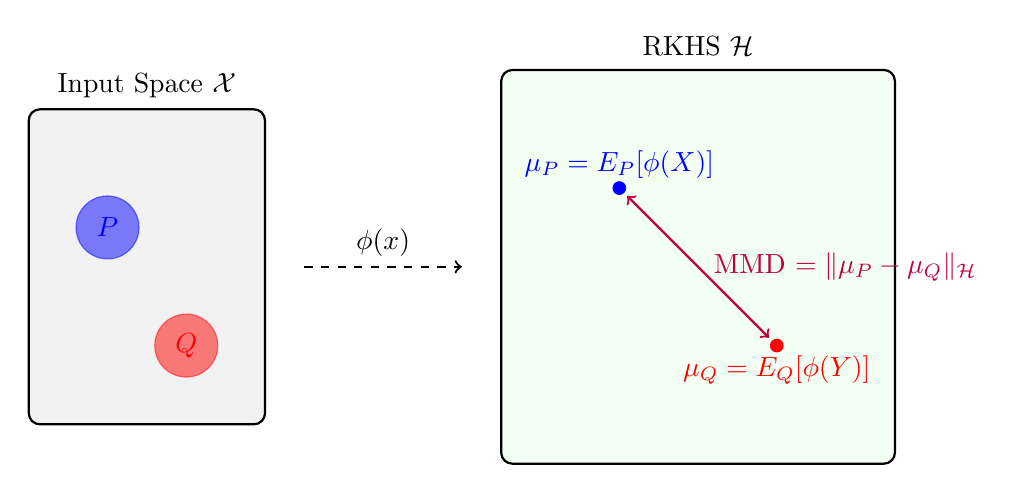
\begin{tikzpicture}
    % Input Space
    \draw[thick, fill=gray!10, rounded corners] (-4, -2) rectangle (-1, 2);
    \node at (-2.5, 2.3) {Input Space $\mathcal{X}$};
    
    \filldraw[blue, opacity=0.5] (-3, 0.5) circle (0.4);
    \node[blue] at (-3, 0.5) {$P$};
    
    \filldraw[red, opacity=0.5] (-2, -1) circle (0.4);
    \node[red] at (-2, -1) {$Q$};

    % Mapping arrow
    \draw[->, thick, dashed] (-0.5, 0) -- (1.5, 0) node[midway, above] {$\phi(x)$};

    % RKHS
    \draw[thick, fill=green!5, rounded corners] (2, -2.5) rectangle (7, 2.5);
    \node at (4.5, 2.8) {RKHS $\mathcal{H}$};

    \filldraw[blue] (3.5, 1) circle (0.08) node[above] {$\mu_P = \mathbb{E}_P[\phi(X)]$};
    \filldraw[red] (5.5, -1) circle (0.08) node[below] {$\mu_Q = \mathbb{E}_Q[\phi(Y)]$};

    \draw[<->, thick, purple] (3.6, 0.9) -- (5.4, -0.9) node[midway, right=2pt] {MMD $= \| \mu_P - \mu_Q \|_{\mathcal{H}}$};

\end{tikzpicture}
\caption{MMD conceptually maps distributions $P$ and $Q$ into a Reproducing Kernel Hilbert Space via feature map $\phi$. The MMD is simply the distance between their mean embeddings $\mu_P$ and $\mu_Q$ in this high-dimensional space.}
\label{fig:mmd_rkhs}
\end{figure}

\subsection{Numerical Example: Empirical MMD}

Suppose we have two finite samples $X = \{x_1, x_2\} \sim P$ and $Y = \{y_1, y_2\} \sim Q$, with $x_1 = 0, x_2 = 1$ and $y_1 = 2, y_2 = 3$.
We choose a linear kernel $k(a, b) = a \cdot b$.

The empirical squared MMD is an unbiased estimator given by:
\begin{equation}
    \widehat{\text{MMD}}^2 = \frac{1}{n(n-1)} \sum_{i \neq j} k(x_i, x_j) + \frac{1}{m(m-1)} \sum_{i \neq j} k(y_i, y_j) - \frac{2}{nm} \sum_{i=1}^n \sum_{j=1}^m k(x_i, y_j).
\end{equation}

For $X = \{0, 1\}$, $x_1 x_2 + x_2 x_1 = 0 + 0 = 0$. So the first term is $0 / 2 = 0$.
For $Y = \{2, 3\}$, $y_1 y_2 + y_2 y_1 = 6 + 6 = 12$. The second term is $12 / 2 = 6$.
For the cross-term, the sum is $(0 \cdot 2) + (0 \cdot 3) + (1 \cdot 2) + (1 \cdot 3) = 0 + 0 + 2 + 3 = 5$. The third term is $-2 \cdot (5 / 4) = -2.5$.

Thus, $\widehat{\text{MMD}}^2 = 0 + 6 - 2.5 = 3.5$. 
The distance reflects the shift in the mean between the two samples, cleanly captured by the linear kernel (where the mean embedding is just the standard mean). With more complex kernels (like Gaussian RBF), MMD can detect differences in variance and higher moments.

\begin{horizon}
While traditional IPMs like MMD and Wasserstein distance require carefully crafted function classes (RKHS balls, Lipschitz continuous functions), modern generative modeling increasingly relies on \textit{Neural IPMs}. In this setting, the discriminator class $\mathcal{F}$ is explicitly parameterized by a deep neural network, $\mathcal{F}_\Theta = \{ f_\theta \mid \theta \in \Theta \}$. 

It is conjectured that when $\mathcal{F}_\Theta$ is appropriately overparameterized, it possesses sufficient capacity to approximate the true Wasserstein-1 distance (provided strict Lipschitz constraints are enforced via spectral normalization or gradient penalties). However, an open question remains regarding the statistical sample complexity of Neural IPMs in extremely high dimensions. Theoretical bounds for traditional IPMs depend heavily on the Rademacher complexity of $\mathcal{F}$, which is notoriously loose for neural networks. 

Future work might show precisely how the implicit bias of gradient descent on the discriminator network constrains its effective capacity, potentially yielding much tighter generalization bounds than those derived from worst-case bounds on the entire neural network hypothesis class. Closing this gap would provide a rigorous foundation for why highly parameterized GANs do not immediately collapse to empirically memorizing the training data, and would firmly link neural empirical distributions with true underlying data manifolds.
\end{horizon}

\section{Summary}
In this chapter, we stepped away from density-based divergences and introduced Integral Probability Metrics (IPMs). By redefining distance as the maximum discrepancy over a class of test functions, IPMs provide continuous, well-behaved metrics even when distributions lack overlapping support. We proved that symmetric function classes yield a simplified IPM definition, and demonstrated that constraining the function class yields classical distances: 1-Lipschitz functions yield the Wasserstein-1 distance, while the unit ball of an RKHS yields the Maximum Mean Discrepancy (MMD). Crucially, MMD admits a closed-form solution via kernel embeddings, bypassing complex optimization.

\section{Exercises}

\begin{enumerate}
    \item \textbf{Total Variation as an IPM:} Let $\mathcal{F}_{\text{TV}}$ be the set of all measurable functions $f$ such that $\sup_x |f(x)| \le 1$. Show that the IPM induced by $\mathcal{F}_{\text{TV}}$ is equal to $\sup_{A \in \Sigma} |P(A) - Q(A)|$, up to a constant scalar factor. 
    \item \textbf{MMD with a Linear Kernel:} Prove that if the kernel is $k(x, y) = x^\top y$, the Maximum Mean Discrepancy $\text{MMD}(P, Q)$ reduces exactly to the Euclidean distance between the expected values (means) of the two distributions, $\| \mathbb{E}[X] - \mathbb{E}[Y] \|_2$.
    \item \textbf{Translational Invariance:} Let $P$ and $Q$ be distributions on $\mathbb{R}^d$. Let $P_c$ and $Q_c$ be the identical distributions shifted by a constant vector $c \in \mathbb{R}^d$. Prove that the Wasserstein-1 distance is translationally invariant: $W_1(P, Q) = W_1(P_c, Q_c)$.
    \item \textbf{Discriminator Optimization:} In the context of a Neural IPM, suppose $\mathcal{F}$ is parametrized by $f_\theta$. Formulate the exact loss function $\mathcal{L}(\theta)$ you would maximize to estimate the IPM between a fixed dataset $X \sim P$ and a generator producing $Y \sim Q$. How does this compare to the standard GAN discriminator loss?
\end{enumerate}

% TODO-CITE: Ensure all named results are cited.

\chapter{Generative Adversarial Networks (GANs)}
\label{ch:gan}

At the heart of unsupervised learning lies the ambition to model the underlying probability distribution of observed data. Given a dataset $\mathcal{D} = \{x_1, \dots, x_N\}$ drawn independent and identically distributed from an unknown, high-dimensional distribution $P_{\text{data}}$ over a space $\mathcal{X}$, the standard statistical approach involves specifying a parameterized family of distributions $p_\theta(x)$ and finding the parameters $\theta$ that maximize the likelihood of the data. This framework, known as prescribed generative modeling, is elegant and enjoys the robust statistical guarantees of maximum likelihood estimation. However, it is historically fraught with computational hurdles. Evaluating the likelihood often requires computing intractable normalizing constants (partition functions), forcing practitioners to rely on approximations like Markov Chain Monte Carlo or to impose overly restrictive structural assumptions (such as strict independence or Gaussianity) to remain tractable. 

Generative Adversarial Networks (GANs) eschew explicit density estimation entirely, offering a radical departure from classical statistics. Instead of prescribing a stochastic decoder distribution $p_\theta(x|z)$ as we did with Variational Autoencoders (see Chapter 13), GANs construct an \textit{implicit} generative model. We define a latent variable $z \in \mathcal{Z}$ with a simple, known prior distribution $p(z)$ (such as a spherical Gaussian), and a deterministic, differentiable function---typically a neural network $f_\theta$---denoted here as the generator $G_\theta : \mathcal{Z} \to \mathcal{X}$, which maps the latent noise into the data space. 

By passing the easily sampled noise $z$ through this complex, non-linear transformation, the distribution of the generated samples $x = G_\theta(z)$ induces an implicit probability measure $P_\theta$ over $\mathcal{X}$. We can easily draw samples from $P_\theta$, but we have no way to evaluate the point-wise density $p_\theta(x)$. The goal of learning is to find parameters $\theta$ such that $P_\theta$ closely approximates $P_{\text{data}}$, matching all of its higher-order moments and topological features.

Because $P_\theta$ does not provide an explicit analytical formula for the likelihood of a point $x$, we cannot directly minimize classical metrics like the Kullback-Leibler (KL) divergence via standard maximum likelihood. To bridge this gap, GANs introduce a second neural network: the \textit{discriminator} $D_\phi : \mathcal{X} \to (0, 1)$. The discriminator is a binary classifier trained to distinguish between true samples drawn from $P_{\text{data}}$ and fake samples drawn from $P_\theta$. Simultaneously, the generator $G_\theta$ is trained to fool the discriminator, updating its parameters to make its synthetic outputs indistinguishable from the real data.

This dual-network architecture fundamentally reframes density estimation as a two-player minimax game. Rather than specifying a static, pre-defined distance metric between distributions, the discriminator acts as an adaptive critic. It dynamically learns the topology of the space where $P_{\text{data}}$ and $P_\theta$ differ most, and penalizes the generator specifically along those axes. As the generator improves and its outputs become more realistic, the discriminator is forced to learn ever more subtle statistical distinctions. This escalating arms race provides a continuously updating, rich gradient signal to the generator.

The adversarial framework shifts the burden from analytical tractability to optimization over function spaces. It is a profound conceptual pivot: we substitute the calculation of an intractable integral with the optimization of an auxiliary neural network. While this trade-off allows GANs to generate astonishingly sharp, high-fidelity samples that capture the manifold structure of complex data (such as photorealistic human faces), it replaces the convex stability of maximum likelihood with the volatile dynamics of non-cooperative game theory.

In this chapter, we formalize the GAN framework. We dissect the core minimax objective, proving that under ideal nonparametric conditions, the game perfectly recovers $P_{\text{data}}$ by implicitly minimizing the Jensen-Shannon Divergence. We then rigorously examine the gradients of this game, shedding light on the catastrophic failure modes---such as vanishing gradients and mode collapse---that plague empirical GAN training when the supports of $P_{\text{data}}$ and $P_\theta$ are disjoint. This analysis sets the stage for the mathematically robust integral probability metrics and $f$-divergences explored in subsequent chapters.

\section{The Minimax Game and Implicit Distributions}

Let $\mathcal{X}$ be the data space and $\mathcal{Z}$ be the latent space. We are given a target distribution $P_{\text{data}}$ over $\mathcal{X}$ and a simple prior $p(z)$ over $\mathcal{Z}$. The generator $G_\theta: \mathcal{Z} \to \mathcal{X}$ pushes forward the measure $p(z)$ to induce a generated distribution $P_\theta$ on $\mathcal{X}$. The discriminator $D_\phi: \mathcal{X} \to (0, 1)$ outputs the probability that a sample $x$ originates from $P_{\text{data}}$ rather than $P_\theta$.

The two networks are pitted against each other in a zero-sum game defined by the value function $V(G_\theta, D_\phi)$:
\begin{equation}
    \min_\theta \max_\phi V(G_\theta, D_\phi) = \mathbb{E}_{x \sim P_{\text{data}}} [\log D_\phi(x)] + \mathbb{E}_{z \sim p(z)} [\log (1 - D_\phi(G_\theta(z)))].
\end{equation}

By the law of the unconscious statistician, we can rewrite the second expectation in terms of the induced distribution $P_\theta$:
\begin{equation}
    V(G_\theta, D_\phi) = \mathbb{E}_{x \sim P_{\text{data}}} [\log D_\phi(x)] + \mathbb{E}_{x \sim P_\theta} [\log (1 - D_\phi(x))].
\end{equation}

To understand the theoretical properties of this game, we study it in the nonparametric limit, assuming both $G_\theta$ and $D_\phi$ have infinite capacity and can represent any measurable function.

\begin{figure}[htpb]
\centering
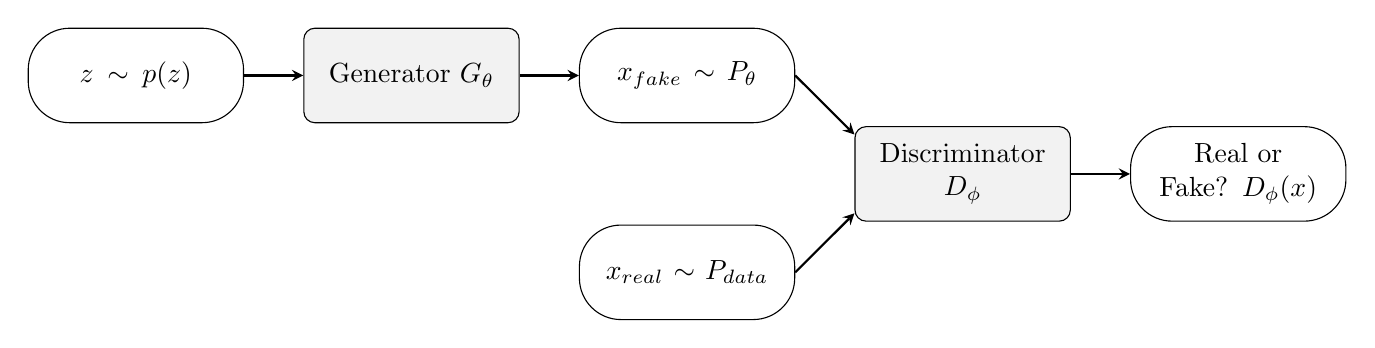
\begin{tikzpicture}[
    box/.style={draw, rectangle, minimum width=2.5cm, minimum height=1.2cm, fill=gray!10, rounded corners, text width=2.5cm, align=center},
    ell/.style={draw, rectangle, rounded corners=15pt, minimum width=2.5cm, minimum height=1.2cm, text width=2.5cm, align=center},
    arr/.style={-stealth, thick}
]
    % Nodes
    \node (z) at (0, 0) [ell] {$z \sim p(z)$};
    \node (G) at (3.5, 0) [box] {Generator $G_\theta$};
    \node (xfake) at (7, 0) [ell] {$x_{\text{fake}} \sim P_\theta$};
    
    \node (xreal) at (7, -2.5) [ell] {$x_{\text{real}} \sim P_{\text{data}}$};
    
    \node (D) at (10.5, -1.25) [box] {Discriminator $D_\phi$};
    
    \node (out) at (14, -1.25) [ell] {Real or Fake? $D_\phi(x)$};
    
    % Arrows
    \draw[arr] (z) -- (G);
    \draw[arr] (G) -- (xfake);
    \draw[arr] (xfake.east) -- (D.160);
    \draw[arr] (xreal.east) -- (D.200);
    \draw[arr] (D) -- (out);
\end{tikzpicture}
\caption{The Generative Adversarial Network architecture. The discriminator $D_\phi$ acts as a learned loss function for the generator $G_\theta$.}
\label{fig:gan_arch}
\end{figure}

\section{Global Optimality and the Jensen-Shannon Divergence}

We first determine the optimal strategy for the discriminator given any fixed generator. Let $p_{\text{data}}(x)$ and $p_\theta(x)$ denote the probability density functions of $P_{\text{data}}$ and $P_\theta$, respectively.

\begin{theorem}[Optimal Discriminator]
\label{thm:optimal_d}
For any fixed generator distribution $P_\theta$ with density $p_\theta(x)$, the optimal discriminator $D^*_\theta(x)$ that maximizes $V(G_\theta, D)$ is given by:
\begin{equation}
    D^*_\theta(x) = \frac{p_{\text{data}}(x)}{p_{\text{data}}(x) + p_\theta(x)}.
\end{equation}
\end{theorem}

\begin{proof}
For a fixed $G_\theta$, the discriminator's objective is to maximize $V(G_\theta, D)$. Writing the expectations as integrals over $\mathcal{X}$, we have:
\begin{align*}
    V(G_\theta, D) &= \int_{\mathcal{X}} p_{\text{data}}(x) \log D(x) \, dx + \int_{\mathcal{X}} p_\theta(x) \log (1 - D(x)) \, dx \\
    &= \int_{\mathcal{X}} \Big[ p_{\text{data}}(x) \log D(x) + p_\theta(x) \log (1 - D(x)) \Big] dx.
\end{align*}
Because $D$ can represent any function, we can maximize the integrand point-wise for every $x \in \mathcal{X}$. Consider a function $f(y) = a \log y + b \log (1 - y)$ for $y \in (0, 1)$ and constants $a, b \ge 0$ (excluding the trivial case $a=b=0$). The derivative with respect to $y$ is:
\begin{equation}
    \frac{df}{dy} = \frac{a}{y} - \frac{b}{1 - y}.
\end{equation}
Setting the derivative to zero yields the maximum at $y^* = \frac{a}{a + b}$. Substituting $a = p_{\text{data}}(x)$ and $b = p_\theta(x)$, the optimal discriminator value for any $x$ is exactly $D^*_\theta(x) = \frac{p_{\text{data}}(x)}{p_{\text{data}}(x) + p_\theta(x)}$. 
\end{proof}

With the optimal discriminator characterized, we can study the generator's objective. By substituting $D^*_\theta$ back into the value function, we expose the underlying divergence metric that GANs implicitly minimize.

\begin{theorem}[Global Optimality of the Generator]
\label{thm:global_g}
The global minimum of the virtual training criterion $C(G_\theta) = \max_{D} V(G_\theta, D)$ is achieved if and only if $P_\theta = P_{\text{data}}$. At this optimal point, $C(G_\theta) = -\log 4$.
\end{theorem}

\begin{proof}
Substitute the optimal discriminator $D^*_\theta(x)$ into $V(G_\theta, D)$:
\begin{align*}
    C(G_\theta) &= \mathbb{E}_{x \sim P_{\text{data}}} \left[ \log \frac{p_{\text{data}}(x)}{p_{\text{data}}(x) + p_\theta(x)} \right] + \mathbb{E}_{x \sim P_\theta} \left[ \log \frac{p_\theta(x)}{p_{\text{data}}(x) + p_\theta(x)} \right].
\end{align*}
To frame this in terms of standard divergences, we multiply the numerator and denominator inside the logarithms by $\frac{1}{2}$:
\begin{align*}
    C(G_\theta) &= \mathbb{E}_{x \sim P_{\text{data}}} \left[ \log \left( \frac{p_{\text{data}}(x)}{\frac{p_{\text{data}}(x) + p_\theta(x)}{2}} \cdot \frac{1}{2} \right) \right] + \mathbb{E}_{x \sim P_\theta} \left[ \log \left( \frac{p_\theta(x)}{\frac{p_{\text{data}}(x) + p_\theta(x)}{2}} \cdot \frac{1}{2} \right) \right] \\
    &= -\log 4 + D_{\text{KL}}\left(P_{\text{data}} \parallel \frac{P_{\text{data}} + P_\theta}{2}\right) + D_{\text{KL}}\left(P_\theta \parallel \frac{P_{\text{data}} + P_\theta}{2}\right).
\end{align*}
This sum of Kullback-Leibler divergences is exactly twice the Jensen-Shannon Divergence ($D_{\text{JSD}}$):
\begin{equation}
    C(G_\theta) = -\log 4 + 2 \cdot D_{\text{JSD}}(P_{\text{data}} \parallel P_\theta).
\end{equation}
Since $D_{\text{JSD}}(P \parallel Q) \ge 0$ for any two distributions and is zero if and only if $P = Q$, the global minimum of $C(G_\theta)$ is $-\log 4$, occurring precisely when $P_\theta = P_{\text{data}}$.
\end{proof}

\section{Vanishing Gradients and the Saturation Regime}

While the minimax formulation guarantees that $P_\theta$ will converge to $P_{\text{data}}$ given optimal discriminators and infinite capacity, practical gradient descent often fails dramatically. To understand why, we must examine the gradients passed from the discriminator to the generator.

The minimax generator loss is defined as:
\begin{equation}
    \mathcal{L}_G(\theta) = \mathbb{E}_{z \sim p(z)} [\log(1 - D_\phi(G_\theta(z)))].
\end{equation}
Let us analyze the gradient of this loss with respect to a generated sample $x = G_\theta(z)$:
\begin{equation}
    \nabla_x \log(1 - D_\phi(x)) = \frac{-1}{1 - D_\phi(x)} \nabla_x D_\phi(x).
\end{equation}

Early in training, the generator's output is poor, meaning $P_\theta$ and $P_{\text{data}}$ are disjoint or highly distinct. Consequently, the discriminator rapidly learns to perfectly separate them, yielding $D_\phi(G_\theta(z)) \approx 0$. As $D_\phi(x) \to 0$, the term $\frac{-1}{1 - D_\phi(x)}$ approaches $-1$. The discriminator function $D_\phi(x)$ becomes extremely flat (due to the saturation of its output sigmoid function) near the generated samples, causing $\nabla_x D_\phi(x) \to 0$. Thus, the generator receives a vanishing gradient exactly when it most needs a strong signal to improve.

To circumvent this, practitioners replace the minimax generator loss with the \textit{nonsaturating} generator loss:
\begin{equation}
    \mathcal{\tilde{L}}_G(\theta) = -\mathbb{E}_{z \sim p(z)} [\log(D_\phi(G_\theta(z)))].
\end{equation}
Here, the gradient with respect to $x$ is:
\begin{equation}
    \nabla_x [-\log D_\phi(x)] = \frac{-1}{D_\phi(x)} \nabla_x D_\phi(x).
\end{equation}
When $D_\phi(x) \to 0$ early in training, the magnitude $\frac{1}{D_\phi(x)} \to \infty$. This amplification counters the flatness of $\nabla_x D_\phi(x)$, providing a massive, non-vanishing gradient signal to the generator.

\begin{figure}[htpb]
\centering
\begin{tikzpicture}[scale=1.2]
    % Axes
    \draw[->, thick] (0, -4.5) -- (0, 2.5) node[above] {Generator Loss};
    \draw[->, thick] (0, 0) -- (5.5, 0) node[right] {$D_\phi(G(z))$};
    
    % Ticks
    \draw (5, 0.1) -- (5, -0.1) node[below] {$1$};
    \node[below left] at (0,0) {$0$};
    
    % Minimax loss: log(1-x)
    \draw[thick, red, dashed, domain=0:4.95, samples=100] plot (\x, {ln(1 - \x/5)});
    
    % Nonsaturating loss: -log(x)
    \draw[thick, blue, domain=0.05:5, samples=100] plot (\x, {-ln(\x/5)});
    
    % Legend
    \node[red, anchor=west] at (2.5, -2) {Minimax: $\log(1-D)$};
    \node[blue, anchor=west] at (1.5, 1.8) {Nonsaturating: $-\log(D)$};
\end{tikzpicture}
\caption{Comparison of generator loss functions. Early in training, the discriminator assigns low probability to fake samples ($D_\phi(G(z)) \approx 0$). The minimax loss (red, dashed) is flat in this regime, yielding vanishing gradients. The nonsaturating loss (blue, solid) exhibits an asymptote at $0$, providing strong initial gradients to propel training.}
\label{fig:gan_loss}
\end{figure}

While the nonsaturating loss resolves the vanishing gradient problem, it changes the theoretical underpinnings of the game. It can be shown that optimizing the nonsaturating loss effectively minimizes a reverse combination of KL divergences. This asymmetric penalty heavily punishes the generation of unrealistic samples but is lenient toward mode dropping, contributing to the empirical phenomenon of \textit{mode collapse} where $P_\theta$ focuses entirely on a small subset of the modes of $P_{\text{data}}$.

\section{Numerical Example: Learning a Gaussian Mean}

To make these pathological gradient mechanics concrete, consider a simple setting where both the true and generated data are one-dimensional Gaussians with unit variance. Let the target distribution be $P_{\text{data}} = \mathcal{N}(\mu^*, 1)$ and the generated distribution be $P_\theta = \mathcal{N}(\theta, 1)$. The generator takes noise $z \sim \mathcal{N}(0, 1)$ and applies the translation $G_\theta(z) = z + \theta$. 

Assuming the discriminator is trained to convergence, we apply Theorem \ref{thm:optimal_d} to find the optimal discriminator:
\begin{equation}
    D^*_\theta(x) = \frac{\exp(-\frac{1}{2}(x - \mu^*)^2)}{\exp(-\frac{1}{2}(x - \mu^*)^2) + \exp(-\frac{1}{2}(x - \theta)^2)}.
\end{equation}
Dividing the numerator and denominator by $\exp(-\frac{1}{2}(x - \mu^*)^2)$, we obtain:
\begin{equation}
    D^*_\theta(x) = \frac{1}{1 + \exp\left( (\mu^* - \theta)x + \frac{1}{2}(\theta^2 - (\mu^*)^2) \right)}.
\end{equation}
This perfectly matches the logistic sigmoid function $D^*_\theta(x) = \sigma(wx + b)$ where the weight is $w = \mu^* - \theta$ and the bias is $b = \frac{1}{2}(\theta^2 - (\mu^*)^2)$.

Let us evaluate the signal received by the generator when it computes the gradient of the standard minimax loss for a generated sample $x = z + \theta$. Note that the derivative of the sample with respect to the parameter is $\frac{\partial x}{\partial \theta} = 1$. By the chain rule, and utilizing the derivative property of the sigmoid function $\sigma'(u) = \sigma(u)(1 - \sigma(u))$:
\begin{align*}
    \nabla_\theta \log(1 - D^*_\theta(G_\theta(z))) &= \frac{-1}{1 - D^*_\theta(x)} \cdot \frac{\partial D^*_\theta(x)}{\partial x} \cdot \frac{\partial x}{\partial \theta} \\
    &= \frac{-1}{1 - D^*_\theta(x)} \Big[ D^*_\theta(x)(1 - D^*_\theta(x)) \cdot w \Big] \cdot 1 \\
    &= -D^*_\theta(x) w \\
    &= D^*_\theta(x) (\theta - \mu^*).
\end{align*}

Consider the regime where the generator is far from the truth, such that $\theta \ll \mu^*$. For a typical fake sample $x \approx \theta$, the discriminator logit evaluated at this sample is:
\begin{equation}
    wx + b = (\mu^* - \theta)\theta + \frac{1}{2}(\theta^2 - (\mu^*)^2) = -\frac{1}{2}(\theta - \mu^*)^2.
\end{equation}
Because the squared distance $(\theta - \mu^*)^2$ is large and positive, the logit is a large negative number, causing the sigmoid output to saturate near zero: $D^*_\theta(x) \approx 0$. 

Consequently, the gradient becomes $\nabla_\theta \log(1 - D^*_\theta) \approx 0 \cdot (\theta - \mu^*) = 0$. The discriminator has perfectly separated the two Gaussians, driving its confidence to 100\% and flattening its decision boundary around the fake samples. Instead of pointing the parameter $\theta$ toward $\mu^*$, the gradient vanishes. This numerically demonstrates the core pathology of the Jensen-Shannon divergence when dealing with disjoint distributions: rather than yielding a gradient proportional to the spatial distance between modes, the gradient decays exponentially, effectively paralyzing the generator.

\begin{horizon}
The fragility of the Jensen-Shannon divergence, illuminated by our Gaussian example, is merely the tip of the topological iceberg. In practice, high-dimensional image distributions $P_{\text{data}}$ and parametrically generated distributions $P_\theta$ are supported on low-dimensional manifolds embedded within a vast ambient space, as posited by the Manifold Hypothesis (Chapter 5). It is conjectured that for any continuous generator mapping, the intersection of these manifolds almost always has measure zero. Thus, a sufficiently powerful discriminator can always achieve perfect separation. Consequently, the true minimax GAN objective is structurally predisposed to gradient starvation in nearly all practical settings.

An open question is whether adversarial training can be mathematically stabilized natively within the standard JSD framework without invoking entirely new distance metrics. While widespread techniques like instance noise, spectral normalization, and gradient penalties artificially enforce Lipschitz continuity on the discriminator---widening its decision boundary to leak signal to the generator---it remains actively debated whether these heuristics secretly optimize alternate mathematical divergences rather than fixing the JSD.

Future work might definitively prove that implicit generative models cannot robustly converge under standard $f$-divergences in high dimensions without exact structural manifold alignment. This limitation strongly motivates the search for metrics that are topologically aware and remain well-defined and differentiable even when supports are disjoint. As we will explore in the upcoming chapters, this realization drives the field's transition from integral probability metrics to optimal transport and Wasserstein distances, fundamentally rewriting the geometric foundations of adversarial learning.
\end{horizon}

\section*{Summary}
\begin{itemize}
    \item Generative Adversarial Networks reframe density estimation as a two-player minimax game, abandoning explicit maximum likelihoods for an implicit generative process $G_\theta(z)$.
    \item Given infinite capacity, the optimal discriminator computes the point-wise ratio of the data density to the combined densities, acting as an adaptive loss function for the generator.
    \item The global optimum of the standard minimax GAN objective occurs when $P_\theta = P_{\text{data}}$, which mathematically corresponds to minimizing the Jensen-Shannon Divergence.
    \item In practice, disjoint distribution supports cause the discriminator to rapidly saturate. This leads to vanishing gradients under the strict minimax loss, forcing the widespread adoption of non-saturating heuristics that alter the convergence dynamics and exacerbate mode collapse.
\end{itemize}

\section*{Exercises}
\begin{enumerate}
    \item \textbf{Optimal Discriminator with Unequal Priors:} Suppose the discriminator is shown real samples with probability $\alpha$ and fake samples with probability $1-\alpha$ (where $\alpha \neq 0.5$). Derive the new optimal discriminator function $D^*_\theta(x)$ that maximizes the modified expected value function.
    \item \textbf{The Nonsaturating Gradient Signal:} Compute the exact gradient $\nabla_\theta [-\log D^*_\theta(G_\theta(z))]$ for the Gaussian example presented in the text. Analyze the behavior of this gradient as $|\theta - \mu^*| \to \infty$. Does it vanish? Prove that it provides a signal pointing toward $\mu^*$.
    \item \textbf{JSD and KL Divergence Bounds:} Prove that $0 \le D_{\text{JSD}}(P \parallel Q) \le \log 2$ for any two probability distributions $P$ and $Q$. Describe the exact conditions under which the upper bound is tight, and connect this to the generator's vanishing gradient problem.
\end{enumerate}

% TODO-CITE: Ensure all named results are cited.

\chapter{$f$-Divergences and their Variational Bounds}
\label{ch:f_divergence}

% 1. Descriptive Opening
In the journey to build machines that can generate complex data---from photorealistic images to coherent human language---a central challenge emerges: how do we measure the distance between the distribution of data our model generates and the true distribution of the world? If we can quantify this discrepancy, we can minimize it. We previously encountered the Kullback-Leibler (KL) divergence, a fundamental measure of relative entropy. However, the KL divergence is just one lens through which to view the difference between distributions. Depending on the nature of the data and the goals of the model, we may want to penalize different types of errors. Should the model cover all modes of the true distribution (mode-covering), even at the risk of generating unrealistic samples? Or should it focus on a single mode (mode-seeking) to ensure high-fidelity outputs, even if it ignores other parts of the data space?

This need for a flexible, parameterized family of statistical distances leads us to the concept of $f$-divergences, introduced independently by Csisz\'{a}r (1967) and Ali and Silvey (1966). An $f$-divergence generalizes the KL divergence by defining the distance between two probability distributions $P$ and $Q$ using a convex function $f$. By choosing different functions for $f$, we recover a wide array of well-known divergences, including the Total Variation distance, the Hellinger distance, the Pearson $\chi^2$ divergence, and the Jensen-Shannon divergence. Each of these distances imposes a distinct geometric structure on the space of probability distributions, dictating how a generative model will behave when optimized to minimize that distance.

However, a significant practical hurdle remains. In the context of deep learning, we rarely have access to the exact probability density functions $P$ and $Q$. Instead, we only have empirical access to samples drawn from these distributions: a dataset $\mathcal{D} \sim P_{\text{data}}$ and a batch of generated samples from $p_\theta(x|z)$. The standard definition of an $f$-divergence involves an integral over the probability densities, which is typically intractable to compute directly in high-dimensional spaces. 

To bridge the gap between the elegant theory of $f$-divergences and the empirical reality of deep learning, we turn to convex analysis, specifically the concept of Fenchel conjugacy. By expressing the convex function $f$ in terms of its convex conjugate $f^*$, we can reformulate the intractable integral of the $f$-divergence into a tractable optimization problem over a family of functions. This mathematical maneuver, heavily popularized in deep learning by the $f$-GAN framework (Nowozin et al., 2016) and the Nguyen-Wainwright-Jordan (NWJ) estimator, transforms the problem of density estimation into a problem of binary classification or density ratio estimation. It provides the theoretical bedrock for understanding why and how adversarial networks---where a discriminator network effectively learns to approximate this variational bound---actually work.

In this chapter, we will rigorously define the family of $f$-divergences, explore their key mathematical properties, and derive their variational bounds. We will see how this variational perspective allows us to estimate these divergences purely from samples, unlocking a unified framework for training generative models.

% 2. Mathematical Core
\section{The Geometry of $f$-Divergences}

Let $P$ and $Q$ be two probability distributions defined over a common measurable space $\mathcal{X}$, such that $P$ is absolutely continuous with respect to $Q$ (denoted $P \ll Q$). This absolute continuity ensures that the Radon-Nikodym derivative, or density ratio, $dP/dQ$ exists. For continuous distributions with probability density functions $p(x)$ and $q(x)$, this ratio is simply $p(x)/q(x)$.

\begin{definition}[$f$-Divergence]
Let $f: (0, \infty) \to \mathbb{R}$ be a convex function such that $f(1) = 0$. Furthermore, suppose $f$ is strictly convex at $1$. The $f$-divergence from distribution $P$ to distribution $Q$ is defined as:
\begin{equation}
    D_f(P \parallel Q) = \int_{\mathcal{X}} q(x) f\left( \frac{p(x)}{q(x)} \right) dx = \mathbb{E}_{x \sim Q} \left[ f\left( \frac{p(x)}{q(x)} \right) \right].
\end{equation}
\end{definition}

The condition $f(1) = 0$ ensures that the divergence between a distribution and itself is zero, $D_f(P \parallel P) = 0$. The convexity of $f$ guarantees that the divergence is non-negative.

\begin{theorem}[Non-negativity of $f$-Divergence]
For any two distributions $P$ and $Q$, and any convex function $f$ with $f(1)=0$, $D_f(P \parallel Q) \ge 0$.
\end{theorem}
\begin{proof}
This is a direct application of Jensen's inequality. Since $f$ is a convex function, we can bring the expectation outside the function:
\begin{align*}
    D_f(P \parallel Q) &= \mathbb{E}_{x \sim Q} \left[ f\left( \frac{p(x)}{q(x)} \right) \right] \\
                       &\ge f\left( \mathbb{E}_{x \sim Q} \left[ \frac{p(x)}{q(x)} \right] \right) \\
                       &= f\left( \int_{\mathcal{X}} q(x) \frac{p(x)}{q(x)} dx \right) \\
                       &= f\left( \int_{\mathcal{X}} p(x) dx \right) \\
                       &= f(1) = 0.
\end{align*}
Equality holds if and only if $p(x) = q(x)$ almost everywhere, provided $f$ is strictly convex around $1$.
\end{proof}

\subsection{A Zoo of Divergences}
By selecting different generator functions $f(u)$, we can instantiate a variety of well-known distance measures. Here we list a few prominent examples:

\begin{itemize}
    \item \textbf{Kullback-Leibler (KL) Divergence}: Let $f(u) = u \log u$. Then $D_f(P \parallel Q) = \int q(x) \frac{p(x)}{q(x)} \log \frac{p(x)}{q(x)} dx = D_{\text{KL}}(P \parallel Q)$.
    \item \textbf{Reverse KL Divergence}: Let $f(u) = -\log u$. Then $D_f(P \parallel Q) = \int q(x) \left(-\log \frac{p(x)}{q(x)}\right) dx = D_{\text{KL}}(Q \parallel P)$.
    \item \textbf{Pearson $\chi^2$ Divergence}: Let $f(u) = (u-1)^2$. Then $D_f(P \parallel Q) = \int q(x) \left(\frac{p(x)}{q(x)} - 1\right)^2 dx = \int \frac{(p(x)-q(x))^2}{q(x)} dx$.
    \item \textbf{Total Variation Distance}: Let $f(u) = \frac{1}{2}|u-1|$. Then $D_f(P \parallel Q) = \frac{1}{2} \int q(x) \left|\frac{p(x)}{q(x)} - 1\right| dx = \frac{1}{2} \int |p(x) - q(x)| dx$.
    \item \textbf{Jensen-Shannon (JS) Divergence}: Let $f(u) = -(u+1)\log\frac{u+1}{2} + u\log u$. This leads to a symmetrized divergence bounded between $0$ and $\log 2$.
\end{itemize}

% TikZ Figure 1: Plotting generator functions f(u)
\begin{figure}[htbp]
\centering
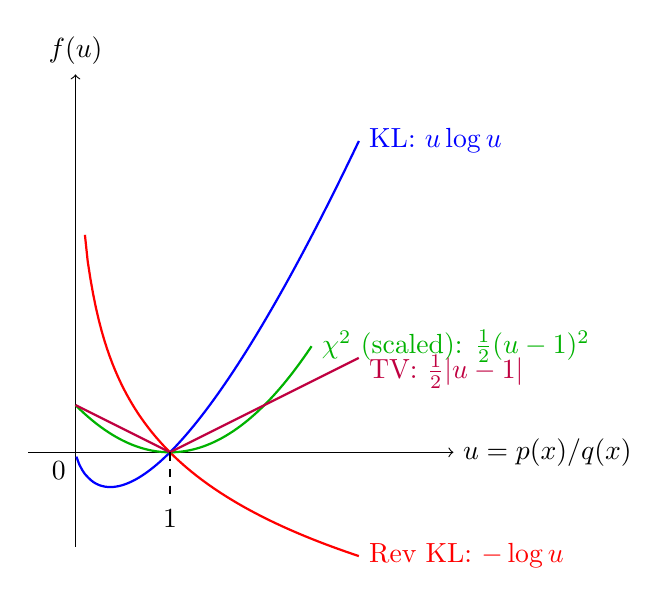
\begin{tikzpicture}[scale=1.2]
    \draw[->] (-0.5,0) -- (4,0) node[right] {$u = p(x)/q(x)$};
    \draw[->] (0,-1) -- (0,4) node[above] {$f(u)$};
    
    % u log u (KL)
    \draw[thick, blue, domain=0.01:3, samples=100] plot (\x, {\x*ln(\x)}) node[right] {KL: $u \log u$};
    
    % -log u (Rev KL)
    \draw[thick, red, domain=0.1:3, samples=100] plot (\x, {-ln(\x)}) node[right] {Rev KL: $-\log u$};
    
    % (u-1)^2 (Pearson chi^2) - scale down a bit for visibility
    \draw[thick, green!70!black, domain=0:2.5, samples=100] plot (\x, {0.5*(\x-1)*(\x-1)}) node[right] {$\chi^2$ (scaled): $\frac{1}{2}(u-1)^2$};
    
    % 0.5|u-1| (Total Variation)
    \draw[thick, purple, domain=0:3, samples=100] plot (\x, {0.5*abs(\x-1)}) node[right, yshift=-5pt] {TV: $\frac{1}{2}|u-1|$};
    
    \draw[dashed] (1,0) -- (1,-0.5) node[below] {$1$};
    \node[below left] at (0,0) {$0$};
\end{tikzpicture}
\caption{Various generator functions $f(u)$ for $f$-divergences. Notice that they all intersect at $f(1)=0$ and are convex.}
\label{fig:f_funcs}
\end{figure}

\section{Variational Bounds via Fenchel Conjugacy}
As noted earlier, calculating $D_f(P \parallel Q)$ requires evaluating an integral over the probability densities. In generative modeling, we typically have access to samples from the data distribution $P$ and the generator distribution $Q$, but not their closed-form densities. To estimate these divergences from samples, we leverage convex duality.

\begin{definition}[Fenchel Conjugate]
Let $f: \mathbb{R} \to \mathbb{R} \cup \{\infty\}$ be a function. Its Fenchel conjugate (or convex conjugate) $f^*: \mathbb{R} \to \mathbb{R} \cup \{\infty\}$ is defined as:
\begin{equation}
    f^*(t) = \sup_{u \in \text{dom}(f)} \left\{ tu - f(u) \right\}.
\end{equation}
\end{definition}

The function $f^*(t)$ is always convex. If $f$ is lower semi-continuous and convex, the Fenchel-Moreau theorem states that the conjugate of the conjugate is the original function: $f^{**}(u) = f(u)$. This implies we can express $f(u)$ as a supremum over $t$:
\begin{equation}
    f(u) = \sup_{t \in \text{dom}(f^*)} \left\{ tu - f^*(t) \right\}.
\end{equation}

\begin{theorem}[Variational Bound on $f$-Divergence]
\label{thm:variational_bound}
Let $P$ and $Q$ be probability distributions on $\mathcal{X}$. Let $f$ be a lower semi-continuous convex function with $f(1)=0$, and let $f^*$ be its convex conjugate. Then, the $f$-divergence can be bounded from below as:
\begin{equation}
    D_f(P \parallel Q) = \sup_{T: \mathcal{X} \to \text{dom}(f^*)} \left( \mathbb{E}_{x \sim P}[T(x)] - \mathbb{E}_{x \sim Q}[f^*(T(x))] \right),
\end{equation}
where the supremum is taken over all measurable functions $T$ mapping from the domain $\mathcal{X}$ to the domain of $f^*$.
\end{theorem}
\begin{proof}
Starting from the definition of the $f$-divergence, we substitute $f$ with its convex conjugate representation:
\begin{align*}
    D_f(P \parallel Q) &= \int_{\mathcal{X}} q(x) f\left( \frac{p(x)}{q(x)} \right) dx \\
                       &= \int_{\mathcal{X}} q(x) \sup_{t} \left\{ t \frac{p(x)}{q(x)} - f^*(t) \right\} dx.
\end{align*}
The supremum inside the integral allows the choice of $t$ to vary for each $x \in \mathcal{X}$. Let us replace the scalar $t$ with a function $T(x)$ that maps each $x$ to a scalar in the domain of $f^*$. By interchanging the integral and the supremum, we get a lower bound (and equality holds for a rich enough class of functions $T$):
\begin{align*}
    D_f(P \parallel Q) &= \sup_{T} \int_{\mathcal{X}} q(x) \left( T(x) \frac{p(x)}{q(x)} - f^*(T(x)) \right) dx \\
                       &= \sup_{T} \left( \int_{\mathcal{X}} p(x) T(x) dx - \int_{\mathcal{X}} q(x) f^*(T(x)) dx \right) \\
                       &= \sup_{T} \left( \mathbb{E}_{x \sim P}[T(x)] - \mathbb{E}_{x \sim Q}[f^*(T(x))] \right).
\end{align*}
This completes the proof.
\end{proof}

The optimal function $T^*(x)$ that achieves this supremum can be found by taking the variation of the functional inside the integral with respect to $T(x)$ and setting it to zero. Using the property that $(f^*)'(t) = (f')^{-1}(t)$ for strictly convex functions, one can show that the optimal discriminator is related to the density ratio:
\begin{equation}
    T^*(x) = f'\left( \frac{p(x)}{q(x)} \right).
\end{equation}

This variational representation is profound. It implies that we can estimate the distance between two distributions by training a neural network $T_\omega(x)$ (a ``discriminator'' or ``critic'' parameterized by $\omega$) to maximize the objective:
\begin{equation}
    \mathcal{L}(\omega) = \mathbb{E}_{x \sim P}[T_\omega(x)] - \mathbb{E}_{x \sim Q}[f^*(T_\omega(x))].
\end{equation}
Once $T_\omega$ is optimized, $\mathcal{L}(\omega)$ serves as an empirical estimate of $D_f(P \parallel Q)$. This is the cornerstone of the $f$-GAN architecture.

% TikZ Figure 2: Conceptual diagram of the variational estimation
\begin{figure}[htbp]
\centering
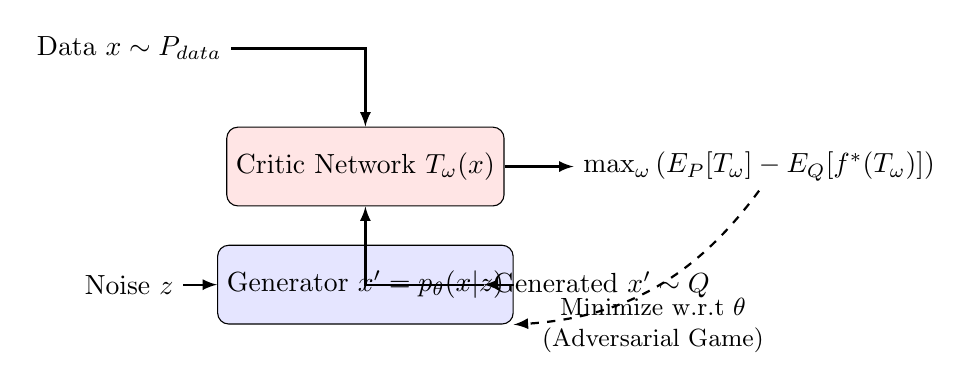
\begin{tikzpicture}[
    box/.style={draw, rounded corners, minimum width=2.5cm, minimum height=1cm, align=center},
    arrow/.style={-latex, thick}
]
    % Nodes
    \node (P) at (0, 3) {Data $x \sim P_{\text{data}}$};
    \node (Z) at (0, 0) {Noise $z$};
    \node[box, fill=blue!10] (G) at (3, 0) {Generator  $x' = p_\theta(x|z)$};
    \node (Q) at (6, 0) {Generated  $x' \sim Q$};
    
    \node[box, fill=red!10] (T) at (3, 1.5) {Critic Network  $T_\omega(x)$};
    
    \node (Obj) at (8, 1.5) {$\max_\omega \left( \mathbb{E}_P[T_\omega] - \mathbb{E}_Q[f^*(T_\omega)] \right)$};

    % Arrows
    \draw[arrow] (Z) -- (G);
    \draw[arrow] (G) -- (Q);
    
    \draw[arrow] (P) -- ++(3,0) -- (T);
    \draw[arrow] (Q) -- ++(-3,0) -- (T);
    
    \draw[arrow] (T) -- (Obj);
    
    % Dashed arrow for generator training
    \draw[arrow, dashed] (Obj.south) to[bend left=25] node[below, align=center, font=\small] {Minimize w.r.t $\theta$\\(Adversarial Game)} (G.south east);
    
\end{tikzpicture}
\caption{The $f$-GAN architecture. A critic network $T_\omega$ is trained to maximize the variational lower bound of the $f$-divergence between the true data distribution $P$ and the generator's distribution $Q$. The generator $p_\theta$ is simultaneously trained to minimize this divergence.}
\label{fig:fgan_arch}
\end{figure}

\subsection{Numerical Example: Deriving the Bound for KL Divergence}
Let's make this concrete by deriving the variational bound for the Kullback-Leibler divergence.
The generator function for KL is $f(u) = u \log u$.
First, we find its Fenchel conjugate $f^*(t)$:
\begin{equation}
    f^*(t) = \sup_{u > 0} \left\{ tu - u \log u \right\}.
\end{equation}
To find the maximum, we take the derivative with respect to $u$ and set it to zero:
\begin{align*}
    \frac{d}{du} (tu - u \log u) &= t - \log u - 1 = 0 \\
    \implies \log u &= t - 1 \\
    \implies u^* &= \exp(t - 1).
\end{align*}
Since the second derivative $-1/u$ is strictly negative for $u>0$, this is a global maximum. Substituting $u^*$ back into the expression yields:
\begin{align*}
    f^*(t) &= t \exp(t-1) - \exp(t-1) \log(\exp(t-1)) \\
           &= t \exp(t-1) - \exp(t-1)(t-1) \\
           &= \exp(t-1).
\end{align*}
Applying Theorem \ref{thm:variational_bound}, the variational bound for KL divergence is:
\begin{equation}
    D_{\text{KL}}(P \parallel Q) = \sup_{T} \left( \mathbb{E}_{x \sim P}[T(x)] - \mathbb{E}_{x \sim Q}[\exp(T(x) - 1)] \right).
\end{equation}
This specific formulation is known as the Nguyen-Wainwright-Jordan (NWJ) bound. 
The optimal critic is $T^*(x) = f'(p(x)/q(x)) = \log(p(x)/q(x)) + 1$. 
If we define a new function $V(x) = T(x) - 1$, the bound becomes the familiar Donsker-Varadhan representation:
\begin{equation}
    D_{\text{KL}}(P \parallel Q) = \sup_{V} \left( \mathbb{E}_{x \sim P}[V(x)] - \mathbb{E}_{x \sim Q}[\exp(V(x)) - 1] \right).
\end{equation}
Notice that the $\log$ is often introduced in practical implementations for numerical stability through Jensen's inequality: $\mathbb{E}[\exp(V(x))] \ge \exp(\mathbb{E}[V(x)])$.

% 3. Horizon Box
\begin{horizon}
While the variational formulation of $f$-divergences provides a mathematically elegant framework for training generative models without explicit densities, it is not without severe practical pathologies. It is conjectured that in high-dimensional spaces, the supports of the true data distribution $P$ and the model distribution $Q$ are often mutually singular---they lie on low-dimensional manifolds that do not perfectly overlap (the Manifold Hypothesis, Chapter 5). 

When $P$ and $Q$ have disjoint supports, the density ratio $p(x)/q(x)$ diverges to infinity or drops to zero. Consequently, most $f$-divergences max out and provide a constant, saturated value. For example, the Jensen-Shannon divergence will quickly saturate to $\log 2$. When the divergence is constant, its gradient with respect to the generator's parameters $\theta$ vanishes. The critic network becomes ``too good'' at distinguishing real from fake data, leaving the generator with no useful learning signal.

An open question is whether one can construct specific $f$-functions that are robust to this dimensional scaling, or if the paradigm inherently fails when supports are disjoint. Future work might show that regularizing the critic's Lipschitz constant implicitly morphs the $f$-divergence into an Integral Probability Metric. Currently, the field has largely shifted toward Wasserstein distances and Optimal Transport (Chapter 24), which naturally handle non-overlapping distributions by measuring the ``cost of moving mass'' rather than relying on point-wise density ratios. Thus, while $f$-divergences are fundamental to information theory, their utility in raw high-dimensional latent spaces may be fundamentally limited.
\end{horizon}

% 4. Summary + Exercises
\section*{Summary}
\begin{itemize}
    \item $f$-divergences provide a generalized family of distance measures between probability distributions, defined by a convex generator function $f$.
    \item Different choices of $f$ lead to well-known divergences like KL, Reverse KL, Jensen-Shannon, and Total Variation, each imposing different behaviors on generative models.
    \item Because computing $f$-divergences directly requires intractable density ratios, we use Fenchel conjugacy to derive a variational lower bound.
    \item This variational bound allows us to estimate the divergence using samples by training a discriminator network $T(x)$, forming the theoretical basis of the $f$-GAN framework.
\end{itemize}

\section*{Exercises}
\begin{enumerate}
    \item \textbf{Deriving the Jensen-Shannon Bound:} Let $f(u) = u \log u - (u+1) \log\left(\frac{u+1}{2}\right)$. Derive the Fenchel conjugate $f^*(t)$ and write out the resulting adversarial objective for estimating the Jensen-Shannon divergence. How does this relate to the original GAN loss proposed by Goodfellow et al. (2014)?
    \item \textbf{Optimal Critic in $\chi^2$ Divergence:} For the Pearson $\chi^2$ divergence where $f(u) = (u-1)^2$, find the Fenchel conjugate $f^*(t)$ and state the variational objective. Show that the optimal critic $T^*(x)$ is exactly $2\left(\frac{p(x)}{q(x)} - 1\right)$. 
    \item \textbf{Vanishing Gradients:} Suppose distributions $P$ and $Q$ are uniform on $[0,1]$ and $[2,3]$ respectively (completely disjoint supports). Compute the KL divergence $D_{\text{KL}}(P \parallel Q)$ and the Jensen-Shannon divergence $D_{\text{JS}}(P \parallel Q)$. What would the gradient of these divergences be if $Q$ was parameterized by a mean $\mu$ (currently at $\mu=2.5$)? Explain why this motivates Wasserstein distances.
\end{enumerate}

% TODO-CITE: Ensure all named results are cited.

\chapter{Optimal Transport and Wasserstein Distances}
\label{chap:optimal_transport}

\section{Introduction}
% Descriptive opening
Information theory provides a rich vocabulary for comparing probability distributions, primarily through divergences such as the Kullback-Leibler (KL) divergence and more generally, $f$-divergences (as explored in Chapter 23). However, these classical divergences suffer from a significant limitation when applied to the kinds of distributions often encountered in deep learning: they require distributions to have overlapping support. When comparing two distributions that are supported on disjoint, low-dimensional manifolds within a high-dimensional ambient space—a common scenario in generative modeling (the Manifold Hypothesis, Chapter 5)—the KL divergence is either undefined or infinite.

Consider the task of evaluating a generative model. We have a target distribution $P_{\text{data}}$ and a generated distribution $P_\theta$. If $P_{\text{data}}$ is a distribution over natural images, it resides on a thin manifold in the pixel space. Early in training, the generated distribution $P_\theta$ is likely supported on a completely different manifold. Because there is no intersection in their supports, the KL divergence provides no useful gradient signal to guide $P_\theta$ towards $P_{\text{data}}$. The divergence simply indicates that the distributions are completely different, without offering a metric of "how far apart" their respective manifolds lie in the ambient space.

This limitation motivates a shift from divergences based on point-wise density ratios to those based on the geometry of the underlying space. This brings us to the mathematical framework of \emph{Optimal Transport} (OT) and the resulting \emph{Wasserstein distances}. Intuitively, optimal transport frames the problem of comparing distributions as a logistics problem: if $P_\theta$ represents a pile of earth (or mass) and $P_{\text{data}}$ represents a hole of equal volume, what is the minimum cost required to transport the mass from $P_\theta$ to fill the hole at $P_{\text{data}}$? 

Because the cost of transport depends on the physical distance the mass must be moved in the ambient space (e.g., Euclidean distance), the Wasserstein distance naturally incorporates the geometry of the underlying metric space. It provides a smooth, meaningful measure of distance even between mutually singular distributions. In deep learning, this geometric awareness was famously leveraged to stabilize the training of Generative Adversarial Networks (GANs), leading to the Wasserstein GAN (WGAN). 

In this chapter, we rigorously develop the theory of optimal transport. We begin with the classical Monge formulation, transition to the Kantorovich relaxation, and define the Wasserstein distance. We then derive the Kantorovich-Rubinstein duality—the crucial mathematical result that makes the Wasserstein distance computationally tractable in deep learning via adversarial training.

\section{The Mathematical Core of Optimal Transport}

\subsection{The Monge Problem}
The study of optimal transport began with Gaspard Monge in 1781. Let $\mathcal{X}$ and $\mathcal{Y}$ be measurable spaces, which in the context of deep learning are typically subsets of $\mathbb{R}^d$. Let $P$ be a probability measure on $\mathcal{X}$ and $Q$ be a probability measure on $\mathcal{Y}$. We define a cost function $c: \mathcal{X} \times \mathcal{Y} \to \mathbb{R}_{\geq 0}$ representing the cost of moving a unit of mass from $x \in \mathcal{X}$ to $y \in \mathcal{Y}$.

A \emph{transport map} is a measurable function $T: \mathcal{X} \to \mathcal{Y}$. We say that $T$ pushes forward $P$ to $Q$, denoted as $T_{\#}P = Q$, if for every measurable set $A \subseteq \mathcal{Y}$, we have:
\[
P(T^{-1}(A)) = Q(A)
\]
The Monge problem seeks to find a transport map $T$ that minimizes the total cost of moving $P$ to $Q$:
\begin{definition}[Monge Problem]
\label{def:monge}
The Monge problem is to find a map $T^*$ such that
\[
T^* = \arg\inf_{T: T_{\#}P = Q} \int_{\mathcal{X}} c(x, T(x)) \, dP(x)
\]
\end{definition}

While intuitively appealing, the Monge problem suffers from severe structural flaws. Specifically, a transport map $T$ must be a deterministic function; it cannot split mass from a single point $x$ to multiple destinations in $\mathcal{Y}$. Consequently, if $P$ is a Dirac delta (a single point mass) and $Q$ is a mixture of two point masses, no valid map $T$ exists such that $T_{\#}P = Q$, rendering the feasible set empty.

\begin{figure}[h]
    \centering
    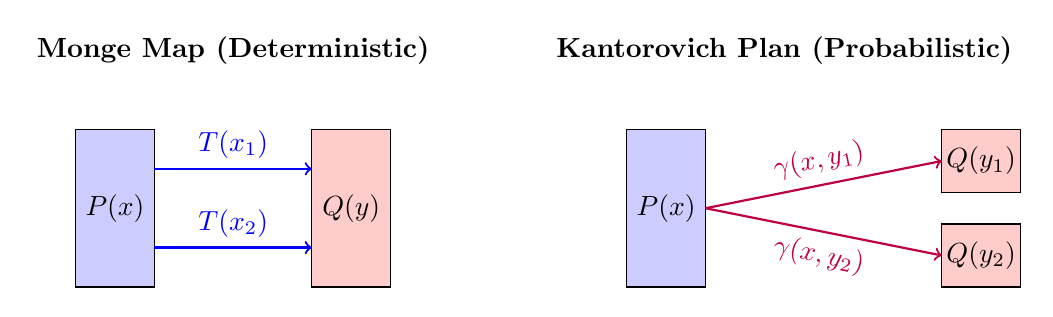
\begin{tikzpicture}
        % Monge Map
        \node at (0,3) {\textbf{Monge Map (Deterministic)}};
        \draw[fill=blue!20] (-2,0) rectangle (-1,2);
        \node at (-1.5,1) {$P(x)$};
        
        \draw[fill=red!20] (1,0) rectangle (2,2);
        \node at (1.5,1) {$Q(y)$};
        
        \draw[->, thick, blue] (-1, 1.5) -- (1, 1.5) node[midway, above] {$T(x_1)$};
        \draw[->, thick, blue] (-1, 0.5) -- (1, 0.5) node[midway, above] {$T(x_2)$};
        
        % Kantorovich Map
        \node at (7,3) {\textbf{Kantorovich Plan (Probabilistic)}};
        \draw[fill=blue!20] (5,0) rectangle (6,2);
        \node at (5.5,1) {$P(x)$};
        
        \draw[fill=red!20] (9,0) rectangle (10,0.8);
        \draw[fill=red!20] (9,1.2) rectangle (10,2);
        \node at (9.5,0.4) {$Q(y_2)$};
        \node at (9.5,1.6) {$Q(y_1)$};
        
        \draw[->, thick, purple] (6, 1) -- (9, 1.6) node[midway, above, sloped] {$\gamma(x, y_1)$};
        \draw[->, thick, purple] (6, 1) -- (9, 0.4) node[midway, below, sloped] {$\gamma(x, y_2)$};
    \end{tikzpicture}
    \caption{The Monge formulation requires deterministic mapping of mass, which can fail if mass must be split. The Kantorovich relaxation introduces a joint distribution (coupling) $\gamma$, allowing mass from a single source to be distributed across multiple targets.}
    \label{fig:monge_kantorovich}
\end{figure}

\subsection{The Kantorovich Relaxation}
To resolve the non-existence of solutions in the Monge problem, Leonid Kantorovich introduced a relaxation in 1942. Instead of finding a deterministic map $T$, Kantorovich proposed finding a \emph{coupling} or \emph{transport plan}—a joint probability measure $\gamma$ on $\mathcal{X} \times \mathcal{Y}$. 

Let $\Pi(P, Q)$ denote the set of all joint probability measures $\gamma$ on $\mathcal{X} \times \mathcal{Y}$ whose marginals are $P$ and $Q$. Mathematically, for any measurable sets $A \subseteq \mathcal{X}$ and $B \subseteq \mathcal{Y}$:
\[
\gamma(A \times \mathcal{Y}) = P(A) \quad \text{and} \quad \gamma(\mathcal{X} \times B) = Q(B)
\]

\begin{definition}[Kantorovich Problem]
\label{def:kantorovich}
The Kantorovich problem is to find a coupling $\gamma^* \in \Pi(P, Q)$ that minimizes the expected cost:
\[
\gamma^* = \arg\inf_{\gamma \in \Pi(P, Q)} \iint_{\mathcal{X} \times \mathcal{Y}} c(x, y) \, d\gamma(x, y)
\]
\end{definition}

The set $\Pi(P, Q)$ is never empty because the independent coupling $\gamma(x, y) = P(x)Q(y)$ always exists. Furthermore, because the objective function is linear in $\gamma$ and the constraint set $\Pi(P, Q)$ is convex and weakly compact, a minimum is guaranteed to exist under mild conditions (e.g., when cost $c$ is lower semi-continuous).

\subsection{The Wasserstein Distance}
When the spaces $\mathcal{X}$ and $\mathcal{Y}$ coincide and form a metric space $(\mathcal{X}, d)$, a natural choice for the cost function is the distance metric raised to a power $p \geq 1$: $c(x, y) = d(x, y)^p$. This choice leads to the formal definition of the Wasserstein distance.

\begin{definition}[$p$-Wasserstein Distance]
\label{def:wasserstein}
Let $(\mathcal{X}, d)$ be a Polish space (a separable completely metrizable space). For $p \geq 1$, the $p$-Wasserstein distance between two probability measures $P$ and $Q$ on $\mathcal{X}$ is defined as:
\[
W_p(P, Q) = \left( \inf_{\gamma \in \Pi(P, Q)} \iint_{\mathcal{X} \times \mathcal{X}} d(x, y)^p \, d\gamma(x, y) \right)^{1/p}
\]
\end{definition}

The Wasserstein distance $W_p$ is a true metric on the space of probability measures with finite $p$-th moments. 
In deep learning, the $1$-Wasserstein distance ($p=1$), often called the Earth Mover's Distance (EMD), is predominantly used. We will denote it simply as $W_1(P, Q)$.

\begin{theorem}[Weak Continuity of Wasserstein Distance]
Unlike the KL divergence, the Wasserstein distance metrizes weak convergence. A sequence of probability measures $(P_n)_{n \in \mathbb{N}}$ converges weakly to $P$ if and only if $W_p(P_n, P) \to 0$ (assuming uniformly integrable $p$-th moments).
\end{theorem}

\begin{proof}
The proof relies on the Portmanteau theorem and is standard in measure theory texts. The key implication for deep learning is that if a sequence of generated distributions $P_\theta$ smoothly approaches a target $P_{\text{data}}$, the Wasserstein distance smoothly decreases to zero, providing a continuous gradient $\nabla_\theta W_1(P_\theta, P_{\text{data}})$.
\end{proof}

\subsection{Numerical Example: Discrete Distributions}
Let us calculate $W_1$ for two simple discrete distributions on $\mathbb{R}$. 
Let $P = \frac{1}{2}\delta_0 + \frac{1}{2}\delta_2$ and $Q = \frac{1}{2}\delta_1 + \frac{1}{2}\delta_3$.
The cost metric is the Euclidean distance $d(x, y) = |x - y|$. 
The joint probability mass function (the coupling $\gamma$) can be represented as a $2 \times 2$ matrix, where rows correspond to the support of $P$ and columns to the support of $Q$. The marginals require row sums to be $1/2$ and column sums to be $1/2$.

The cost matrix $C$ where $C_{ij} = |x_i - y_j|$ is:
\[
C = \begin{pmatrix}
|0-1| & |0-3| \\
|2-1| & |2-3|
\end{pmatrix}
= \begin{pmatrix}
1 & 3 \\
1 & 1
\end{pmatrix}
\]
We want to minimize $\sum_{i,j} \gamma_{ij} C_{ij}$. Let the coupling matrix be $\Gamma$:
\[
\Gamma = \begin{pmatrix}
\gamma_{11} & \gamma_{12} \\
\gamma_{21} & \gamma_{22}
\end{pmatrix}
\]
To satisfy marginal constraints: $\gamma_{11} + \gamma_{12} = 1/2$, $\gamma_{21} + \gamma_{22} = 1/2$, $\gamma_{11} + \gamma_{21} = 1/2$, $\gamma_{12} + \gamma_{22} = 1/2$.
Notice that moving mass from $x=0$ to $y=1$ costs 1, and $x=2$ to $y=3$ costs 1. The total cost under the coupling $\Gamma = \begin{pmatrix} 1/2 & 0 \\ 0 & 1/2 \end{pmatrix}$ is:
\[
W_1(P, Q) = \frac{1}{2}(1) + 0(3) + 0(1) + \frac{1}{2}(1) = 1.
\]
Any other valid coupling, e.g., $\Gamma = \begin{pmatrix} 0 & 1/2 \\ 1/2 & 0 \end{pmatrix}$, yields a cost of $\frac{1}{2}(3) + \frac{1}{2}(1) = 2$. Thus, $W_1(P, Q) = 1$.

\subsection{Kantorovich-Rubinstein Duality}
Evaluating the primal Kantorovich problem directly in high dimensions is intractable due to the infinite-dimensional space of couplings $\Pi(P, Q)$. The pivotal breakthrough that allows Wasserstein distances to be used as objective functions in neural networks is the dual formulation.

\begin{theorem}[Kantorovich-Rubinstein Duality]
\label{thm:kr_duality}
For the $W_1$ distance, the Kantorovich problem admits the following dual representation:
\[
W_1(P, Q) = \sup_{\|f\|_L \leq 1} \mathbb{E}_{x \sim P}[f(x)] - \mathbb{E}_{y \sim Q}[f(y)]
\]
where the supremum is taken over all $1$-Lipschitz functions $f: \mathcal{X} \to \mathbb{R}$. A function $f$ is $1$-Lipschitz if $|f(x) - f(y)| \leq d(x, y)$ for all $x, y \in \mathcal{X}$.
\end{theorem}

\begin{proof}
Let us sketch the derivation using the min-max theorem. The primal problem is a constrained optimization problem. We can enforce the marginal constraints using Lagrange multipliers. Let $f \in L^1(dP)$ and $g \in L^1(dQ)$ be dual variables (functions). 
The Lagrangian is:
\begin{align*}
L(\gamma, f, g) &= \iint c(x,y) d\gamma(x,y) + \int f(x) \left( dP(x) - \int d\gamma(x,y) \right) + \int g(y) \left( dQ(y) - \int d\gamma(x,y) \right) \\
&= \int f(x) dP(x) + \int g(y) dQ(y) + \iint \left( c(x,y) - f(x) - g(y) \right) d\gamma(x,y)
\end{align*}
By the min-max theorem (Slater's condition holds), $\inf_\gamma \sup_{f,g} L = \sup_{f,g} \inf_\gamma L$.
When minimizing over $\gamma \geq 0$, if $c(x,y) - f(x) - g(y) < 0$ for any $x,y$, the inner infimum evaluates to $-\infty$. Therefore, we must constrain $f(x) + g(y) \leq c(x,y)$. Under this constraint, the integral with respect to $\gamma$ vanishes. The problem becomes:
\[
\sup_{f,g: f(x)+g(y) \leq c(x,y)} \int f(x) dP(x) + \int g(y) dQ(y)
\]
For $c(x,y) = d(x,y)$, one can show that the optimal $g$ is $-f$ ($c$-transform), and the constraint $f(x) - f(y) \leq d(x,y)$ implies exactly that $f$ is $1$-Lipschitz. This yields the Kantorovich-Rubinstein formula.
\end{proof}

This duality transforms the search over couplings into a maximization problem over a single scalar-valued function $f$, which in deep learning can be parameterized by a neural network.

\begin{figure}[h]
    \centering
    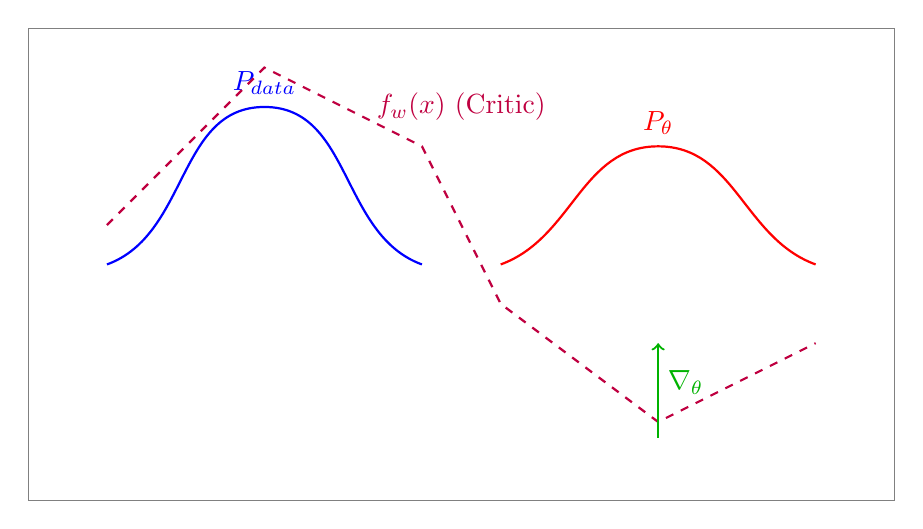
\begin{tikzpicture}
        % Distributions
        \draw[thick, blue] (0,0) to[out=20,in=180] (2,2) to[out=0,in=160] (4,0);
        \node[blue] at (2,2.3) {$P_{\text{data}}$};
        
        \draw[thick, red] (5,0) to[out=20,in=180] (7,1.5) to[out=0,in=160] (9,0);
        \node[red] at (7,1.8) {$P_\theta$};
        
        % Lipschitz function f
        \draw[thick, dashed, purple] (0, 0.5) -- (2, 2.5) -- (4, 1.5) -- (5, -0.5) -- (7, -2) -- (9, -1);
        \node[purple] at (4.5, 2) {$f_w(x)$ (Critic)};
        
        % Arrows indicating gradients
        \draw[->, thick, green!70!black] (7,-2.2) -- (7,-1);
        \node[green!70!black, right] at (7,-1.5) {$\nabla_\theta$};
        
        % Box
        \draw[gray, thin] (-1,-3) rectangle (10, 3);
    \end{tikzpicture}
    \caption{In the Wasserstein GAN framework, a neural network $f_w$ (the critic) acts as the dual function. It is trained to maximize the difference in expectations between $P_{\text{data}}$ and $P_\theta$ subject to a Lipschitz constraint. The gradients of this critic then smoothly push the generator's distribution $P_\theta$ towards $P_{\text{data}}$.}
    \label{fig:wgan_critic}
\end{figure}

In the context of the Wasserstein GAN, the function $f$ (often parameterized with weights $w$, so $f_w$) is called the \emph{critic} rather than the discriminator, because it outputs a real-valued score rather than a probability. The generator, parametrized by $\theta$, minimizes the Wasserstein distance estimated by the critic.

\section{Horizon}
\begin{horizon}
The mathematical elegance of the Kantorovich-Rubinstein duality fundamentally reoriented generative modeling. However, enforcing the $1$-Lipschitz constraint globally on a neural network remains a severe theoretical and practical challenge. Existing methods, such as gradient penalty or weight normalization, enforce the constraint only locally along the interpolation path or restrict the capacity of the network in poorly understood ways.

It is conjectured that the set of functions achievable by standard deep neural networks (with ReLU or similar piecewise linear activations) under strict global Lipschitz bounds may be pathologically constrained, lacking the expressivity to accurately compute the supremum in the dual formulation for complex distributions. An open question is whether a fundamentally different architecture or parameterization could perfectly capture the space of $1$-Lipschitz functions in high dimensions without collapsing the model's capacity.

Future work might show that alternative geometric formulations, such as those relying on entropic regularization (e.g., the Sinkhorn divergence), will supersede the strict dual approach. Entropic OT replaces the hard Lipschitz constraint with a soft entropic penalty, yielding computationally robust, differentiable distance metrics that naturally interpolate between maximum mean discrepancy and optimal transport, potentially providing the definitive metric space for the next generation of deep learning representations.
\end{horizon}

\section{Summary and Exercises}
In this chapter, we identified the failure modes of density-based divergences when dealing with mutually singular distributions supported on disjoint manifolds. We formalized the geometry-aware framework of optimal transport, beginning with the restrictive Monge problem and moving to the probabilistically relaxed Kantorovich formulation. By defining the Wasserstein distance and leveraging the Kantorovich-Rubinstein duality, we established a tractable objective function that computes continuous gradients even when distributions do not overlap.

\subsection*{Exercises}
\begin{enumerate}
    \item \textbf{Translation Invariance:} Prove that for a shift $c \in \mathbb{R}^d$, $W_p(P, Q) = W_p(P_c, Q_c)$ where $P_c$ is the distribution of $X+c$ for $X \sim P$.
    \item \textbf{The 1D Case:} For continuous distributions on the real line $\mathbb{R}$ with cumulative distribution functions $F(x)$ and $G(y)$, prove that the $p$-Wasserstein distance has the closed-form solution:
    \[ W_p^p(P, Q) = \int_0^1 |F^{-1}(u) - G^{-1}(u)|^p \, du \]
    where $F^{-1}$ and $G^{-1}$ are the quantile functions.
    \item \textbf{Lipschitz Enforcement:} Compare clipping weights (as originally proposed in WGAN) versus gradient penalty ($L= (\|\nabla f(x)\|_2 - 1)^2$) in terms of bounding the Lipschitz constant of $f$. Why does weight clipping artificially constrain the functional capacity more severely?
\end{enumerate}

% TODO-CITE: Ensure all named results are cited.


\part{Score Matching and Diffusion Models}
\chapter{Score-Based Generative Modeling}
\label{chap:score_matching}

\section{The Geometry of Probability: Beyond the Partition Function}

The central ambition of generative modeling is to discover a mathematical representation of the underlying data distribution, $p_{\text{data}}(x)$, from which a given dataset $\mathcal{D} = \{x_1, \dots, x_N\}$ is assumed to be drawn independently and identically distributed. Historically, this endeavor has been dominated by the principle of maximum likelihood estimation (MLE). In the MLE paradigm, we posit a parameterized family of distributions $p_\theta(x)$ and seek the parameters $\theta$ that maximize the probability of the observed data.

However, the seemingly straightforward application of MLE is often frustrated by a fundamental architectural constraint. Many expressive families of probability distributions, particularly Energy-Based Models (EBMs), are defined up to an intractable normalization constant. An EBM defines the probability density as
\begin{equation}
    p_\theta(x) = \frac{e^{-E_\theta(x)}}{Z_\theta},
\end{equation}
where $E_\theta(x)$ is a parameterized scalar function referred to as the \textit{energy}, and $Z_\theta = \int e^{-E_\theta(x)} dx$ is the \textit{partition function}. The partition function ensures that the probability density integrates to one, a non-negotiable requirement of probability theory. Yet, computing $Z_\theta$ requires an integral over the entire high-dimensional data space $\mathcal{X}$, which is computationally prohibitive for spaces of even moderate dimensionality, such as images or text.

To bypass the partition function, we must shift our perspective from the absolute value of the probability density to its local geometry. Consider the spatial derivative of the log-probability density with respect to the data itself:
\begin{equation}
    \nabla_x \log p_\theta(x) = \nabla_x \left( -E_\theta(x) - \log Z_\theta \right) = -\nabla_x E_\theta(x).
\end{equation}
Because $Z_\theta$ is a constant with respect to $x$, its derivative vanishes. This vector field, $\nabla_x \log p(x)$, is known as the \textit{score function} (not to be confused with the Fisher score in statistics, which is the gradient with respect to the parameters $\theta$). 

The score function offers a profoundly different geometric interpretation of a probability distribution. While the density $p(x)$ assigns a scalar mass to every point in space, the score function assigns a vector pointing in the direction of the steepest ascent of the log-density. Intuitively, if one were placed at an arbitrary point in the data space, the score vector would indicate the direction to walk in order to reach more probable, "data-like" configurations. A generative model that accurately learns this vector field learns the fundamental structure of the data manifold. We can subsequently use this learned vector field to draw new samples by simulating a particle that stochastically follows the score vectors towards regions of high probability.

This approach, known as \textit{score-based generative modeling} or \textit{score matching}, liberates us from the tyranny of the partition function. We can train a neural network $s_\theta(x)$ to directly approximate the score function of the data distribution, $\nabla_x \log p_{\text{data}}(x)$, without ever explicitly modeling the density $p_\theta(x)$. However, a new challenge immediately arises: we do not have access to the true data score function $\nabla_x \log p_{\text{data}}(x)$. We only have empirical samples. The mathematical core of this chapter concerns how we can nonetheless train a network to match this unknown vector field.

\section{The Score Function and Fisher Divergence}

To formally learn the score function, we need an appropriate distance metric between our model's score $s_\theta(x)$ and the true data score $\nabla_x \log p_{\text{data}}(x)$. The natural choice is the expected squared Euclidean distance, a quantity deeply related to the Fisher divergence.

\begin{definition}[Fisher Divergence]
Let $P$ and $Q$ be two strictly positive, continuously differentiable probability distributions on $\mathbb{R}^d$. The Fisher divergence from $P$ to $Q$ is defined as
\begin{equation}
    D_F(P \parallel Q) = \mathbb{E}_{x \sim P} \left[ \left\| \nabla_x \log P(x) - \nabla_x \log Q(x) \right\|_2^2 \right].
\end{equation}
\end{definition}

In our context, we wish to minimize $J(\theta) = \frac{1}{2} D_F(p_{\text{data}} \parallel p_\theta)$, where we substitute a neural network $s_\theta(x)$ for $\nabla_x \log p_\theta(x)$. The explicit score matching objective is thus:
\begin{equation}
    J_{\text{ESM}}(\theta) = \frac{1}{2} \mathbb{E}_{x \sim p_{\text{data}}} \left[ \left\| s_\theta(x) - \nabla_x \log p_{\text{data}}(x) \right\|_2^2 \right].
\end{equation}
As noted, this objective is intractable because $\nabla_x \log p_{\text{data}}(x)$ is unknown. Remarkably, Aapo Hyvärinen demonstrated that this objective can be rewritten in a form that only depends on the data distribution via expectations over the samples, eliminating the need for the true score.

\begin{theorem}[Implicit Score Matching]
\label{thm:implicit_score_matching}
Assume that $p_{\text{data}}(x)$ is continuously differentiable and that $p_{\text{data}}(x) \|s_\theta(x)\|_2 \to 0$ as $\|x\|_2 \to \infty$. Then, minimizing $J_{\text{ESM}}(\theta)$ is equivalent to minimizing the implicit score matching objective $J_{\text{ISM}}(\theta)$, defined as:
\begin{equation}
    J_{\text{ISM}}(\theta) = \mathbb{E}_{x \sim p_{\text{data}}} \left[ \operatorname{tr}(\nabla_x s_\theta(x)) + \frac{1}{2} \|s_\theta(x)\|_2^2 \right],
\end{equation}
up to an additive constant that is independent of $\theta$. Here, $\nabla_x s_\theta(x)$ is the Jacobian matrix of the network, and $\operatorname{tr}$ denotes the trace operator.
\end{theorem}

\begin{proof}
We begin by expanding the squared Euclidean norm in the explicit score matching objective:
\begin{align*}
    J_{\text{ESM}}(\theta) &= \frac{1}{2} \int p_{\text{data}}(x) \left\| s_\theta(x) - \nabla_x \log p_{\text{data}}(x) \right\|_2^2 dx \\
    &= \int p_{\text{data}}(x) \left( \frac{1}{2}\|s_\theta(x)\|_2^2 - \langle s_\theta(x), \nabla_x \log p_{\text{data}}(x) \rangle + \frac{1}{2}\|\nabla_x \log p_{\text{data}}(x)\|_2^2 \right) dx.
\end{align*}
The third term $\frac{1}{2}\|\nabla_x \log p_{\text{data}}(x)\|_2^2$ is independent of $\theta$, so we can absorb it into a constant $C$. We now focus on the cross term:
\begin{align*}
    -\int p_{\text{data}}(x) \langle s_\theta(x), \nabla_x \log p_{\text{data}}(x) \rangle dx &= -\int p_{\text{data}}(x) \sum_{i=1}^d s_{\theta, i}(x) \frac{\partial}{\partial x_i} \log p_{\text{data}}(x) dx \\
    &= -\int \sum_{i=1}^d s_{\theta, i}(x) \frac{\partial}{\partial x_i} p_{\text{data}}(x) dx,
\end{align*}
where we utilized the identity $\nabla_x \log p(x) = \frac{\nabla_x p(x)}{p(x)}$.
We apply integration by parts to each dimension $i$:
\begin{equation}
    \int s_{\theta, i}(x) \frac{\partial}{\partial x_i} p_{\text{data}}(x) dx = \left[ s_{\theta, i}(x) p_{\text{data}}(x) \right]_{-\infty}^{\infty} - \int p_{\text{data}}(x) \frac{\partial}{\partial x_i} s_{\theta, i}(x) dx.
\end{equation}
By the assumption that $p_{\text{data}}(x) \|s_\theta(x)\|_2 \to 0$ as $x \to \pm\infty$, the boundary term evaluates to zero. Thus, the cross term simplifies to:
\begin{equation}
    \int \sum_{i=1}^d p_{\text{data}}(x) \frac{\partial}{\partial x_i} s_{\theta, i}(x) dx = \mathbb{E}_{x \sim p_{\text{data}}} \left[ \sum_{i=1}^d \frac{\partial s_{\theta, i}(x)}{\partial x_i} \right] = \mathbb{E}_{x \sim p_{\text{data}}} \left[ \operatorname{tr}(\nabla_x s_\theta(x)) \right].
\end{equation}
Substituting this back into the expanded objective yields $J_{\text{ISM}}(\theta) + C$, completing the proof.
\end{proof}

\begin{figure}[htbp]
\centering
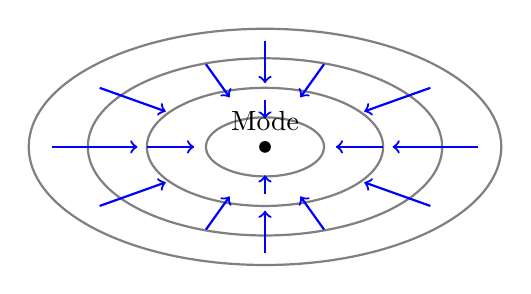
\begin{tikzpicture}[scale=1.5]
    % Draw some contours
    \draw[gray, thick] (0,0) ellipse (2 and 1);
    \draw[gray, thick] (0,0) ellipse (1.5 and 0.75);
    \draw[gray, thick] (0,0) ellipse (1 and 0.5);
    \draw[gray, thick] (0,0) ellipse (0.5 and 0.25);
    
    % Draw score vectors (gradient of log prob)
    \foreach \x/\y in {
        1.8/0, -1.8/0, 0/0.9, 0/-0.9,
        1.4/0.5, -1.4/-0.5, -1.4/0.5, 1.4/-0.5,
        1/0, -1/0, 0/0.4, 0/-0.4,
        0.5/0.7, -0.5/-0.7, 0.5/-0.7, -0.5/0.7
    } {
        \draw[->, blue, thick] (\x,\y) -- ({0.6*\x}, {0.6*\y});
    }
    
    \node[circle, fill=black, inner sep=1.5pt, label=above:Mode] at (0,0) {};
\end{tikzpicture}
\caption{The score function $\nabla_x \log p(x)$ forms a vector field that points toward the modes (regions of high density) of the probability distribution. The arrows are orthogonal to the level sets of the density.}
\label{fig:score_field}
\end{figure}

While Theorem \ref{thm:implicit_score_matching} provides a theoretically sound objective, it presents severe computational hurdles in the context of deep learning. The term $\operatorname{tr}(\nabla_x s_\theta(x))$ requires computing the trace of the Jacobian matrix of the network with respect to the inputs. For a $d$-dimensional input, this naïvely requires $d$ backward passes through the network. While Hutchinson's trace estimator can approximate this term, implicit score matching still struggles empirically, particularly because the objective provides poor learning signals in low-density regions where data samples are scarce.

\section{Denoising Score Matching}

To circumvent the computational cost of the Jacobian trace and provide a robust learning signal everywhere, Vincent (2011) introduced Denoising Score Matching (DSM). The core insight is that adding a small amount of noise to the data smooths out the distribution, filling in low-density regions, and profoundly simplifying the score matching objective.

Let us define a predefined noise distribution $q_\sigma(\tilde{x}|x) = \mathcal{N}(\tilde{x}; x, \sigma^2 I)$. The perturbed data distribution is the marginal:
\begin{equation}
    q_\sigma(\tilde{x}) = \int q_\sigma(\tilde{x}|x) p_{\text{data}}(x) dx.
\end{equation}
Instead of matching the score of the original data, we aim to match the score of this perturbed distribution, $\nabla_{\tilde{x}} \log q_\sigma(\tilde{x})$.

\begin{theorem}[Denoising Score Matching]
\label{thm:denoising_score_matching}
Minimizing the explicit score matching objective for the perturbed distribution $q_\sigma(\tilde{x})$:
\begin{equation}
    J_{\text{SM}}(\theta; \sigma) = \frac{1}{2} \mathbb{E}_{\tilde{x} \sim q_\sigma(\tilde{x})} \left[ \left\| s_\theta(\tilde{x}) - \nabla_{\tilde{x}} \log q_\sigma(\tilde{x}) \right\|_2^2 \right],
\end{equation}
is equivalent to minimizing the denoising score matching objective:
\begin{equation}
    J_{\text{DSM}}(\theta; \sigma) = \frac{1}{2} \mathbb{E}_{x \sim p_{\text{data}}} \mathbb{E}_{\tilde{x} \sim q_\sigma(\tilde{x}|x)} \left[ \left\| s_\theta(\tilde{x}) - \nabla_{\tilde{x}} \log q_\sigma(\tilde{x}|x) \right\|_2^2 \right],
\end{equation}
up to an additive constant independent of $\theta$.
\end{theorem}

\begin{proof}
We expand $J_{\text{SM}}(\theta; \sigma)$:
\begin{equation}
    J_{\text{SM}}(\theta; \sigma) = \frac{1}{2} \mathbb{E}_{q_\sigma(\tilde{x})} [\|s_\theta(\tilde{x})\|_2^2] - \mathbb{E}_{q_\sigma(\tilde{x})} [\langle s_\theta(\tilde{x}), \nabla_{\tilde{x}} \log q_\sigma(\tilde{x}) \rangle] + C_1.
\end{equation}
Let us focus on the cross term. Using the identity $q_\sigma(\tilde{x}) \nabla_{\tilde{x}} \log q_\sigma(\tilde{x}) = \nabla_{\tilde{x}} q_\sigma(\tilde{x})$, we have:
\begin{align*}
    \mathbb{E}_{q_\sigma(\tilde{x})} [\langle s_\theta(\tilde{x}), \nabla_{\tilde{x}} \log q_\sigma(\tilde{x}) \rangle] &= \int \langle s_\theta(\tilde{x}), \nabla_{\tilde{x}} q_\sigma(\tilde{x}) \rangle d\tilde{x} \\
    &= \int \left\langle s_\theta(\tilde{x}), \nabla_{\tilde{x}} \int p_{\text{data}}(x) q_\sigma(\tilde{x}|x) dx \right\rangle d\tilde{x} \\
    &= \iint p_{\text{data}}(x) \langle s_\theta(\tilde{x}), \nabla_{\tilde{x}} q_\sigma(\tilde{x}|x) \rangle dx d\tilde{x} \\
    &= \iint p_{\text{data}}(x) q_\sigma(\tilde{x}|x) \langle s_\theta(\tilde{x}), \nabla_{\tilde{x}} \log q_\sigma(\tilde{x}|x) \rangle dx d\tilde{x} \\
    &= \mathbb{E}_{x \sim p_{\text{data}}} \mathbb{E}_{\tilde{x} \sim q_\sigma(\tilde{x}|x)} [\langle s_\theta(\tilde{x}), \nabla_{\tilde{x}} \log q_\sigma(\tilde{x}|x) \rangle].
\end{align*}
Now, consider the expansion of $J_{\text{DSM}}(\theta; \sigma)$:
\begin{equation}
    J_{\text{DSM}}(\theta; \sigma) = \frac{1}{2} \mathbb{E}_{x, \tilde{x}} [\|s_\theta(\tilde{x})\|_2^2] - \mathbb{E}_{x, \tilde{x}} [\langle s_\theta(\tilde{x}), \nabla_{\tilde{x}} \log q_\sigma(\tilde{x}|x) \rangle] + C_2.
\end{equation}
Because the marginal of $\tilde{x}$ over the joint distribution is $q_\sigma(\tilde{x})$, the first term $\mathbb{E}_{x, \tilde{x}} [\|s_\theta(\tilde{x})\|_2^2]$ is identical to $\mathbb{E}_{q_\sigma(\tilde{x})} [\|s_\theta(\tilde{x})\|_2^2]$. Since we have shown the cross terms are also equivalent, the two objectives differ only by a constant $(C_1 - C_2)$ that does not depend on $\theta$.
\end{proof}

\begin{figure}[htbp]
\centering
\begin{tikzpicture}[scale=1.5]
    % Data manifold (a curve)
    \draw[very thick, black] (-2, -1) .. controls (-1, 1) and (1, -1) .. (2, 1) node[right] {Data Manifold $\mathcal{M}$};
    
    % Points on manifold
    \node[circle, fill=black, inner sep=1.5pt] (x) at (0, 0) {};
    \node[below right] at (x) {$x \sim p_{\text{data}}$};
    
    % Corrupted points
    \node[circle, fill=red, inner sep=1.5pt] (xtilde1) at (-0.5, 0.8) {};
    \node[above] at (xtilde1) {$\tilde{x} \sim q_\sigma(\tilde{x}|x)$};
    
    \node[circle, fill=red, inner sep=1.5pt] (xtilde2) at (0.6, -0.6) {};
    
    % Arrows from corrupted points back to manifold (score)
    \draw[->, blue, thick, shorten >= 2pt] (xtilde1) -- (x);
    \draw[->, blue, thick, shorten >= 2pt] (xtilde2) -- (x);
    
    % Noise distribution circle
    \draw[dashed, red] (x) circle (0.94); % 0.94 is roughly distance to xtilde1
\end{tikzpicture}
\caption{Denoising Score Matching. Clean data points $x$ on a low-dimensional manifold are perturbed to $\tilde{x}$. Because the noise distribution $q_\sigma(\tilde{x}|x)$ is Gaussian, its score $\nabla_{\tilde{x}} \log q_\sigma(\tilde{x}|x) = (x - \tilde{x}) / \sigma^2$ is a vector pointing exactly from the noisy point back to the clean point. The network learns to act as a denoiser.}
\label{fig:denoising}
\end{figure}

The brilliance of DSM lies in the analytical tractability of the conditional score. For Gaussian noise $q_\sigma(\tilde{x}|x) \propto \exp(-\frac{\|\tilde{x} - x\|_2^2}{2\sigma^2})$, the conditional score is simply:
\begin{equation}
    \nabla_{\tilde{x}} \log q_\sigma(\tilde{x}|x) = -\frac{\tilde{x} - x}{\sigma^2}.
\end{equation}
Substituting this into $J_{\text{DSM}}$, the objective becomes a simple mean squared error between the network's output and the noise vectors. The network acts as a vector field pointing from perturbed points back towards their clean origins on the data manifold, effectively functioning as a denoiser.

\section{Numerical Example: Isotropic Gaussian}

To build intuition, let us derive the true score for a simple case and observe what the network must learn. Consider a target distribution that is an isotropic Gaussian, $p_{\text{data}}(x) = \mathcal{N}(x; \mu, \sigma_d^2 I)$. 

The density is:
\begin{equation}
    p_{\text{data}}(x) = \frac{1}{(2\pi \sigma_d^2)^{d/2}} \exp\left( -\frac{\|x - \mu\|_2^2}{2\sigma_d^2} \right).
\end{equation}
Taking the logarithm:
\begin{equation}
    \log p_{\text{data}}(x) = -\frac{\|x - \mu\|_2^2}{2\sigma_d^2} - \frac{d}{2} \log(2\pi \sigma_d^2).
\end{equation}
The true score function is the gradient:
\begin{equation}
    \nabla_x \log p_{\text{data}}(x) = -\frac{x - \mu}{\sigma_d^2}.
\end{equation}
This is a linear vector field pointing precisely towards the mean $\mu$, with a magnitude proportional to the distance from the mean, scaled inversely by the variance. If we parameterize a neural network $s_\theta(x) = W x + b$, implicit score matching would recover $W = -\frac{1}{\sigma_d^2}I$ and $b = \frac{\mu}{\sigma_d^2}$. 

\begin{horizon}
The mathematical equivalence of Denoising Score Matching implies a profound connection between score functions and information theory, crystallized in the celebrated de Bruijn identity. The identity states that the derivative of the Shannon differential entropy of a random variable undergoing Gaussian diffusion is precisely proportional to its Fisher information: $\frac{d}{d\sigma^2} h(X + \mathcal{N}(0, \sigma^2 I)) = \frac{1}{2} J(X + \mathcal{N}(0, \sigma^2 I))$. 

It is conjectured that the empirical success of multi-scale score matching (using an annealed noise schedule $\sigma_1 > \sigma_2 > \dots > \sigma_L$) is not merely a numerical trick, but fundamentally tied to the optimal transport of information. Future work might show that the optimal noise schedule for training diffusion models rigorously minimizes the rate of information loss per step, mapping exactly onto bounds derived in non-equilibrium thermodynamics for the minimal dissipation of work. An open question is whether the Information Bottleneck principle can be explicitly embedded into the score matching objective to bound the generalization error of generative sampling.
\end{horizon}

\section{Summary}
In this chapter, we explored the paradigm of score-based generative modeling, which shifts the focus from estimating normalized probability densities to estimating the score function—the gradient of the log-density. This sidesteps the intractable partition function. We proved that while direct score matching requires computationally expensive trace operations (Implicit Score Matching), the objective can be elegantly reformulated into Denoising Score Matching. By adding Gaussian noise, the network learns to denoise, which corresponds exactly to estimating the score of the smoothed data distribution. This mathematical framework provides the critical foundation for the continuous-time diffusion models explored in subsequent chapters.

\section*{Exercises}
\begin{enumerate}
    \item \textbf{Jacobian Trace for Multilayer Perceptrons.} Consider a 2-layer MLP $s_\theta(x) = W_2 \phi(W_1 x + b_1) + b_2$ where $\phi$ is an element-wise activation function. Derive the analytical expression for the trace term $\operatorname{tr}(\nabla_x s_\theta(x))$ required in Implicit Score Matching. What is the computational complexity compared to evaluating $s_\theta(x)$?
    \item \textbf{Score of a Gaussian Mixture.} Let $p(x) = \frac{1}{2}\mathcal{N}(x; \mu_1, \Sigma_1) + \frac{1}{2}\mathcal{N}(x; \mu_2, \Sigma_2)$. Compute the exact score function $\nabla_x \log p(x)$. Show analytically that the score function evaluates to a non-linear combination of the individual cluster scores, heavily weighted towards the nearest cluster mode.
    \item \textbf{Variance of the DSM Estimator.} While Denoising Score Matching is unbiased with respect to the explicit score matching gradient, its empirical variance can be high for small $\sigma$. Prove that as $\sigma \to 0$, the variance of the stochastic gradient of $J_{\text{DSM}}$ approaches infinity, explaining the necessity of perturbing the data significantly during training.
\end{enumerate}

% TODO-CITE: Ensure all named results are cited.

\chapter{Langevin Dynamics and Fokker-Planck Equations}
\label{ch:langevin}

\section{The Physical Intuition of Generative Diffusion}

The previous chapter introduced score-based generative modeling as a mechanism for learning the gradient fields of data distributions. While the empirical success of mapping noise to data via score functions is undeniable, a rigorous mathematical framework is required to formalize this process. To build this foundation, we turn to non-equilibrium statistical mechanics, specifically the study of particles suspended in a fluid subject to thermal fluctuations.

In physics, the macroscopic behavior of a diffusing substance (like a drop of ink in water) is fundamentally connected to the microscopic, erratic trajectories of individual particles. The mathematician Paul Langevin described the microscopic perspective by modeling the motion of a single particle under the influence of two competing forces: a deterministic drift pushing the particle down a potential energy gradient, and a stochastic diffusion caused by random collisions with fluid molecules. The continuous-time stochastic process describing this particle's trajectory is known as \emph{Langevin dynamics}.

When we transpose this physical model into the realm of deep generative learning, the "particle" becomes a single data point navigating a high-dimensional space $\mathcal{X}$. The "potential energy landscape" is defined by the negative log-likelihood of our data distribution, $U(x) = -\log p_{\text{data}}(x)$. The deterministic drift force pulling the particle toward regions of low energy is therefore precisely the score function: $-\nabla U(x) = \nabla \log p_{\text{data}}(x)$. This drift continuously pulls the state toward the high-density manifolds of the data. 

Simultaneously, the "thermal noise" injected into the system acts as an exploratory force. Without noise, particles would deterministically fall into the nearest local maximum of the data density and halt, resulting in mode collapse. The continuous injection of Brownian noise prevents the particle from becoming permanently trapped in spurious local optima, ensuring that the system explores the entire state space and samples from the global probability distribution in exact proportion to $p_{\text{data}}(x)$.

While Langevin dynamics characterizes the microscopic path of a single point $X_t$, it is often more illuminating to track the macroscopic evolution of an entire ensemble of particles. If we initialize a cloud of particles from an arbitrary prior distribution and let each undergo independent Langevin dynamics, how does the probability density of the cloud, $p_t(x)$, evolve over time? The deterministic partial differential equation governing this evolving density is the \emph{Fokker-Planck equation} (also known in probability theory as the Kolmogorov forward equation). 

The Fokker-Planck equation is the bridge between the microscopic stochasticity of data generation and the macroscopic determinism of probability distributions. By leveraging this equation, we can mathematically prove that the stationary state of Langevin dynamics is exactly the true data distribution. Furthermore, from an information-theoretic perspective, we can demonstrate that the entropy of the system evolves in a strictly monotonic fashion, continuously dissipating the Kullback-Leibler divergence between the current distribution and the target data distribution. In this chapter, we formalize these dynamics and establish the continuous-time backbone upon which modern diffusion models operate.

\section{Mathematical Primer: Measure Theory and It\^o Calculus}

The transition from discrete Markov chains to continuous-time stochastic processes requires a fundamental shift in our mathematical toolkit. In discrete time, a random walk is easily understood as a sequence of random variables. However, if we attempt to take the continuous-time limit by shrinking the step size to zero while maintaining a finite variance, the resulting trajectories exhibit pathological behavior: they become continuous everywhere but differentiable nowhere. 

To formalize such processes, we cannot rely on standard Riemann calculus. Instead, we must turn to measure theory and It\^o calculus. Measure theory provides the rigorous foundation for defining probabilities over uncountably infinite dimensional path spaces. The central object of this theory for our purposes is the Wiener measure, which formalizes the distribution of standard Brownian motion.

\begin{definition}[Standard Brownian Motion]
A standard $d$-dimensional Brownian motion, or Wiener process, is a continuous-time stochastic process $\{W_t\}_{t \ge 0}$ characterized by three properties:
\begin{enumerate}
    \item $W_0 = 0$ almost surely.
    \item For any $0 \le s < t$, the increment $W_t - W_s$ is independent of the past values $W_u$ for all $0 \le u \le s$.
    \item The increments are normally distributed: $W_t - W_s \sim \mathcal{N}(0, (t-s)I)$.
\end{enumerate}
\end{definition}

Because the increments of Brownian motion scale with $\sqrt{\Delta t}$ rather than $\Delta t$, the quadratic variation of $W_t$ over a time interval is non-zero. Consequently, the standard rules of classical calculus fail. If we apply a smooth nonlinear function to a stochastic process, the traditional chain rule does not hold. 

To analyze the temporal evolution of such systems, we must use It\^o calculus, which extends classical calculus by incorporating the second-order effects of stochastic fluctuations. 

\begin{lemma}[It\^o's Lemma]
Let $X_t$ be a $d$-dimensional It\^o process governed by the stochastic differential equation $dX_t = \mu(X_t, t) dt + \sigma(X_t, t) dW_t$. For any twice continuously differentiable function $f(x, t) : \mathbb{R}^d \times \mathbb{R} \to \mathbb{R}$, the differential of $f(X_t, t)$ is given by:
\begin{equation}
    df = \left( \frac{\partial f}{\partial t} + \nabla_x f^\top \mu + \frac{1}{2} \text{Tr}\left( \sigma \sigma^\top \nabla^2_x f \right) \right) dt + \nabla_x f^\top \sigma \, dW_t
\end{equation}
\end{lemma}

The crucial addition in It\^o's Lemma is the second-order trace term involving the Hessian $\nabla^2_x f$. This term captures the macroscopic drift generated by the accumulation of microscopic variance. With these mathematical tools established, we can now rigorously define our continuous-time generative dynamics.

\section{Langevin Dynamics and Stochastic Differential Equations}

We begin by formally defining the continuous-time process. Let $X_t \in \mathbb{R}^d$ be a random variable representing the state of our generative process at time $t \ge 0$. The evolution of $X_t$ is governed by a Stochastic Differential Equation (SDE) of the form:

\begin{equation}
    dX_t = \mu(X_t, t) dt + \sigma(X_t, t) dW_t
\end{equation}

where $\mu: \mathbb{R}^d \times \mathbb{R} \to \mathbb{R}^d$ is the drift coefficient, $\sigma: \mathbb{R}^d \times \mathbb{R} \to \mathbb{R}^{d \times d}$ is the diffusion coefficient, and $W_t$ is a standard $d$-dimensional Brownian motion (or Wiener process). The Wiener process formally represents the continuous-time limit of a random walk, characterized by continuous paths and independent, normally distributed increments $W_{t+\Delta t} - W_t \sim \mathcal{N}(0, \Delta t I)$.

\begin{definition}[Overdamped Langevin Dynamics]
Let $p_{\text{data}}(x)$ be a continuously differentiable target probability density on $\mathbb{R}^d$. The \emph{overdamped Langevin dynamics} associated with $p_{\text{data}}$ is the SDE given by:
\begin{equation}
    dX_t = \nabla \log p_{\text{data}}(X_t) dt + \sqrt{2} dW_t
\end{equation}
\end{definition}

In this specific SDE, the drift term is the score function $\mu(X_t, t) = \nabla \log p_{\text{data}}(X_t)$, which points in the direction of steepest ascent in the data density. The diffusion matrix is constant, $\sigma(X_t, t) = \sqrt{2} I$. The constant $\sqrt{2}$ is carefully chosen to balance the deterministic drift and the stochastic noise such that the system ultimately converges to $p_{\text{data}}(x)$.

\begin{figure}[htpb]
\centering
\begin{tikzpicture}[scale=1.5]
  % Contours representing the data distribution density
  \draw[thick, blue!20] (0,0) ellipse (2.5cm and 1.8cm);
  \draw[thick, blue!40] (0,0) ellipse (1.8cm and 1.2cm);
  \draw[thick, blue!60] (0,0) ellipse (1.2cm and 0.7cm);
  \draw[thick, blue!80] (0,0) ellipse (0.6cm and 0.35cm);
  
  \node[blue] at (2.0, -1.5) {$\nabla \log p_{\text{data}}(x)$};
  
  % Vector field arrows representing the score (drift)
  \foreach \angle in {0, 45, 90, 135, 180, 225, 270, 315} {
    \draw[->, blue, thick, opacity=0.7] (\angle:2.0cm and 1.3cm) -- (\angle:1.6cm and 1.0cm);
  }
  
  % Langevin Trajectory
  \draw[red, thick, ->] (-2.8, -1.6) 
    -- (-2.4, -1.3) -- (-2.5, -0.9) -- (-1.8, -0.6) 
    -- (-1.5, -0.8) -- (-1.1, -0.4) -- (-1.2, 0.1) 
    -- (-0.6, 0.2) -- (-0.4, 0.0) -- (0.0, 0.1);
  
  \fill[red] (-2.8, -1.6) circle (1.5pt) node[below left] {$X_0 \sim p_0$};
  \fill[red] (0.0, 0.1) circle (1.5pt) node[above right] {$X_t$};
\end{tikzpicture}
\caption{A simulated microscopic trajectory of Langevin dynamics. The particle $X_t$ starts from an initial prior distribution and performs a random walk biased by the score function (blue arrows) toward the high-density regions of $p_{\text{data}}(x)$.}
\label{fig:langevin_trajectory}
\end{figure}


\section{The Fokker-Planck Equation}

To understand how the probability density $p_t(x)$ of the random variable $X_t$ evolves over time, we transition from the microscopic SDE to the macroscopic partial differential equation. 

For a general It\^o SDE $dX_t = \mu(X_t, t) dt + \sigma(X_t, t) dW_t$, the evolution of its marginal probability density function $p_t(x)$ is deterministically governed by the Fokker-Planck equation:
\begin{equation}
    \frac{\partial p_t(x)}{\partial t} = -\sum_{i=1}^d \frac{\partial}{\partial x_i} \left[ \mu_i(x, t) p_t(x) \right] + \frac{1}{2} \sum_{i=1}^d \sum_{j=1}^d \frac{\partial^2}{\partial x_i \partial x_j} \left[ (\sigma(x,t) \sigma(x,t)^\top)_{ij} p_t(x) \right]
\end{equation}
Substituting the specific coefficients for our Langevin dynamics, $\mu(x, t) = \nabla \log p_{\text{data}}(x)$ and $\sigma(x, t) = \sqrt{2} I$, the second-order diffusion tensor becomes $(\sqrt{2} I)(\sqrt{2} I)^\top = 2I$. This simplifies the Fokker-Planck equation to:

\begin{equation}
    \label{eq:langevin_fpe}
    \frac{\partial p_t(x)}{\partial t} = -\nabla \cdot \left( p_t(x) \nabla \log p_{\text{data}}(x) \right) + \Delta p_t(x)
\end{equation}

where $\nabla \cdot (\cdot)$ denotes the divergence operator and $\Delta = \nabla \cdot \nabla$ is the Laplace operator. The first term on the right-hand side represents the advection of the probability mass driven by the score field, effectively concentrating density in modes. The second term, the Laplacian, represents isotropic heat diffusion, effectively smoothing and spreading the probability mass.

\begin{figure}[htpb]
\centering
\begin{tikzpicture}
  \begin{axis}[
      width=12cm, height=6.5cm,
      xlabel=$x$, ylabel={$p_t(x)$},
      domain=-4:4,
      samples=150,
      axis lines=left,
      every axis y label/.style={at={(axis description cs:0,1.05)},anchor=south},
      every axis x label/.style={at={(axis description cs:1.05,0)},anchor=west},
      no marks,
      thick,
      ymax=0.6,
      ymin=0
    ]
    
    % Initial distribution (Prior)
    \addplot[black!60, dashed, thick] {1/(sqrt(2*pi*1.5)) * exp(-x^2/(2*1.5))};
    \node[black!60, right] at (axis cs:0.2, 0.15) {$p_0(x)$ (Prior)};
    
    % Intermediate distribution
    \addplot[orange, thick] {0.4 * 1/(sqrt(2*pi*0.5)) * exp(-(x-1.2)^2/(2*0.5)) + 0.6 * 1/(sqrt(2*pi*0.5)) * exp(-(x+1.2)^2/(2*0.5))};
    \node[orange, right] at (axis cs:1.2, 0.25) {$p_t(x)$ (Intermediate)};
    
    % Target distribution (bimodal)
    \addplot[blue, very thick] {0.4 * 1/(sqrt(2*pi*0.15)) * exp(-(x-2)^2/(2*0.15)) + 0.6 * 1/(sqrt(2*pi*0.15)) * exp(-(x+2)^2/(2*0.15))};
    \node[blue, right] at (axis cs:2.2, 0.45) {$p_{\text{data}}(x)$ (Stationary)};

  \end{axis}
\end{tikzpicture}
\caption{Macroscopic evolution of the probability density according to the Fokker-Planck equation. An initially broad prior density $p_0(x)$ is simultaneously transported and shaped by the score function until it exactly matches the multi-modal stationary target distribution $p_{\text{data}}(x)$.}
\label{fig:fokker_planck_evolution}
\end{figure}

\section{Stationarity of the Data Distribution}

The fundamental reason we employ Langevin dynamics in generative modeling is that its equilibrium state perfectly reconstructs the unknown data distribution. We can rigorously prove this by finding the stationary solution to the Fokker-Planck equation.

\begin{theorem}[Stationary Distribution of Langevin Dynamics]
\label{thm:langevin_stationarity}
Let $p_{\text{data}}(x)$ be a probability density on $\mathbb{R}^d$. If $X_t$ evolves according to the Langevin dynamics $dX_t = \nabla \log p_{\text{data}}(X_t) dt + \sqrt{2} dW_t$, then $p_{\text{data}}(x)$ is a stationary distribution of the process.
\end{theorem}

\begin{proof}
A distribution is stationary if, when the process reaches it, the density no longer changes over time. Mathematically, this requires $\frac{\partial p_t(x)}{\partial t} = 0$. We substitute $p_t(x) = p_{\text{data}}(x)$ into the right-hand side of the Fokker-Planck Equation \eqref{eq:langevin_fpe}:
\begin{align*}
    \frac{\partial p_t(x)}{\partial t} &= -\nabla \cdot \left( p_{\text{data}}(x) \nabla \log p_{\text{data}}(x) \right) + \Delta p_{\text{data}}(x)
\end{align*}
Recall the logarithmic derivative identity: $\nabla p(x) = p(x) \nabla \log p(x)$. Using this identity, we rewrite the advection term:
\begin{align*}
    p_{\text{data}}(x) \nabla \log p_{\text{data}}(x) &= \nabla p_{\text{data}}(x)
\end{align*}
Substituting this back into the divergence operator yields:
\begin{align*}
    \frac{\partial p_t(x)}{\partial t} &= -\nabla \cdot \left( \nabla p_{\text{data}}(x) \right) + \Delta p_{\text{data}}(x) \\
    &= -\Delta p_{\text{data}}(x) + \Delta p_{\text{data}}(x) \\
    &= 0
\end{align*}
Because the time derivative vanishes everywhere, $p_{\text{data}}(x)$ is an invariant measure of the stochastic differential equation.
\end{proof}

\section{Information-Theoretic Convergence: The H-Theorem}

Theorem \ref{thm:langevin_stationarity} proves that if the process reaches $p_{\text{data}}$, it stays there. But does it actually converge to $p_{\text{data}}$ from an arbitrary prior distribution? We can prove convergence by tracking the Kullback-Leibler (KL) divergence $D_{\text{KL}}(p_t \parallel p_{\text{data}})$. This analysis yields a continuous-time analog to the Second Law of Thermodynamics (often referred to as an H-theorem or a generalized de Bruijn's identity).

\begin{theorem}[Monotonic Dissipation of KL Divergence]
\label{thm:kl_dissipation}
Let $p_t(x)$ be the probability density of the state $X_t$ under the Langevin dynamics associated with $p_{\text{data}}(x)$. Assuming suitable regularity conditions such that integration by parts holds and boundary terms vanish at infinity, the KL divergence between $p_t$ and $p_{\text{data}}$ is monotonically non-increasing:
\begin{equation}
    \frac{d}{dt} D_{\text{KL}}(p_t \parallel p_{\text{data}}) \le 0
\end{equation}
\end{theorem}

\begin{proof}
By definition, the KL divergence is:
\begin{align*}
    D_{\text{KL}}(p_t \parallel p_{\text{data}}) &= \int p_t(x) \log \frac{p_t(x)}{p_{\text{data}}(x)} dx
\end{align*}
Taking the time derivative, we apply the Leibniz integral rule:
\begin{align}
    \frac{d}{dt} D_{\text{KL}}(p_t \parallel p_{\text{data}}) &= \int \frac{\partial p_t}{\partial t} \log \frac{p_t}{p_{\text{data}}} dx + \int p_t \frac{\partial}{\partial t} \left( \log p_t - \log p_{\text{data}} \right) dx \nonumber \\
    &= \int \frac{\partial p_t}{\partial t} \log \frac{p_t}{p_{\text{data}}} dx + \int p_t \left( \frac{1}{p_t} \frac{\partial p_t}{\partial t} \right) dx \nonumber \\
    &= \int \frac{\partial p_t}{\partial t} \log \frac{p_t}{p_{\text{data}}} dx + \frac{d}{dt} \int p_t dx \label{eq:kl_deriv}
\end{align}
Because $p_t(x)$ is a valid probability density for all $t$, $\int p_t dx = 1$, making its time derivative zero. We now substitute the Fokker-Planck equation for $\frac{\partial p_t}{\partial t}$. First, we rewrite the FPE in a more convenient form:
\begin{align*}
    \frac{\partial p_t}{\partial t} &= -\nabla \cdot \left( p_t \nabla \log p_{\text{data}} \right) + \nabla \cdot \left( \nabla p_t \right) \\
    &= \nabla \cdot \left( p_t \nabla \log p_t - p_t \nabla \log p_{\text{data}} \right) \\
    &= \nabla \cdot \left( p_t \nabla \log \frac{p_t}{p_{\text{data}}} \right)
\end{align*}
Substituting this back into Equation \eqref{eq:kl_deriv} yields:
\begin{equation*}
    \frac{d}{dt} D_{\text{KL}}(p_t \parallel p_{\text{data}}) = \int \nabla \cdot \left( p_t \nabla \log \frac{p_t}{p_{\text{data}}} \right) \log \frac{p_t}{p_{\text{data}}} dx
\end{equation*}
We now apply multivariate integration by parts (Green's first identity). Assuming the density decays sufficiently fast at infinity, the boundary terms evaluate to zero:
\begin{align*}
    \frac{d}{dt} D_{\text{KL}}(p_t \parallel p_{\text{data}}) &= -\int p_t(x) \left( \nabla \log \frac{p_t(x)}{p_{\text{data}}(x)} \right) \cdot \left( \nabla \log \frac{p_t(x)}{p_{\text{data}}(x)} \right) dx \\
    &= -\int p_t(x) \left\| \nabla \log \frac{p_t(x)}{p_{\text{data}}(x)} \right\|_2^2 dx \\
    &= -\mathbb{E}_{X \sim p_t} \left[ \left\| \nabla \log p_t(X) - \nabla \log p_{\text{data}}(X) \right\|_2^2 \right] \le 0
\end{align*}
This completes the proof. The quantity on the right is exactly the negative \emph{relative Fisher information}. Because it is an expectation of a squared norm, it is strictly non-positive, ensuring that the process irreversibly consumes information until it converges exactly to the target distribution.
\end{proof}


\section{Numerical Example: Discretization Bias}

In practice, a neural network is trained to approximate the score $\nabla \log p_{\text{data}}(x)$, and the continuous-time SDE must be discretized for computer simulation. The most common discretization is the Euler-Maruyama method, which yields the Unadjusted Langevin Algorithm (ULA). For a step size $\epsilon > 0$, the update rule is:
\begin{equation}
    x_{k+1} = x_k + \epsilon \nabla \log p_{\text{data}}(x_k) + \sqrt{2\epsilon} z_k, \quad z_k \sim \mathcal{N}(0, I)
\end{equation}
While continuous Langevin dynamics perfectly matches $p_{\text{data}}$, the discrete-time approximation introduces a fundamental \emph{discretization bias}. We can compute this bias exactly for a simple Gaussian target.

Suppose the data distribution is a zero-mean Gaussian with variance $\sigma^2$: $p_{\text{data}}(x) = \mathcal{N}(0, \sigma^2)$. The exact score is $\nabla \log p_{\text{data}}(x) = -x / \sigma^2$. The ULA update becomes:
\begin{equation}
    x_{k+1} = x_k - \epsilon \frac{x_k}{\sigma^2} + \sqrt{2\epsilon} z_k = \left( 1 - \frac{\epsilon}{\sigma^2} \right) x_k + \sqrt{2\epsilon} z_k
\end{equation}
This is a first-order autoregressive AR(1) process. Taking the variance of both sides and assuming independence between $x_k$ and the noise $z_k$:
\begin{equation}
    \text{Var}(x_{k+1}) = \left( 1 - \frac{\epsilon}{\sigma^2} \right)^2 \text{Var}(x_k) + 2\epsilon \text{Var}(z_k)
\end{equation}
At equilibrium (stationarity), $\text{Var}(x_{k+1}) = \text{Var}(x_k) = v_\infty$. Solving for $v_\infty$:
\begin{align*}
    v_\infty &= \left( 1 - \frac{2\epsilon}{\sigma^2} + \frac{\epsilon^2}{\sigma^4} \right) v_\infty + 2\epsilon \\
    v_\infty \left( \frac{2\epsilon}{\sigma^2} - \frac{\epsilon^2}{\sigma^4} \right) &= 2\epsilon \\
    v_\infty &= \frac{2\epsilon}{\frac{2\epsilon}{\sigma^2} - \frac{\epsilon^2}{\sigma^4}} = \frac{2\sigma^4}{2\sigma^2 - \epsilon} = \sigma^2 \left( \frac{1}{1 - \frac{\epsilon}{2\sigma^2}} \right)
\end{align*}
For a strictly positive step size $\epsilon > 0$ (specifically, $\epsilon < 2\sigma^2$ for stability), the stationary variance $v_\infty$ is strictly greater than the target variance $\sigma^2$. Using a Taylor expansion for small $\epsilon$, $v_\infty \approx \sigma^2 + \frac{\epsilon}{2}$. 

This analysis reveals a stark reality: numerical simulation of Langevin dynamics systematically over-disperses the sampled distribution. In deep generative modeling, this bias manifests as blurry or noisy samples if the step size $\epsilon$ is not carefully annealed to zero over the course of sampling.

\begin{horizon}
The mathematical elegance of Langevin dynamics relies intrinsically on the injection of stochastic noise. However, one of the most remarkable realizations in recent diffusion research is that the \emph{marginal densities} $p_t(x)$ prescribed by the Fokker-Planck equation can be achieved via entirely deterministic trajectories. It is conjectured that for any stochastic differential equation, there exists a corresponding deterministic ordinary differential equation (a Probability Flow ODE) whose continuous-time evolution traces the exact same sequence of marginal distributions, mapping the prior to the data distribution without ever explicitly injecting noise. 

An open question is whether these Probability Flow ODEs can be conceptualized as optimal transport maps, minimizing a specific dynamic cost function (such as the Wasserstein distance) between the prior and data manifolds. Future work might show that instead of simulating thousands of discrete Langevin steps, we can directly regress the vector field of this optimal transport map, effectively "rectifying" the generative flow into a straight line. 

Furthermore, while our derivation assumes a flat Euclidean space $\mathbb{R}^d$, real-world data (such as molecular conformations or climate systems) frequently resides on non-Euclidean manifolds. Extending the Fokker-Planck equation to Riemannian manifolds requires substituting the standard Laplacian with the Laplace-Beltrami operator. It is conjectured that formulating score-matching and Langevin dynamics intrinsically in the geometric space of the data will drastically reduce the discretization bias observed in current models, paving the way for generative physics simulations.
\end{horizon}

\section*{Chapter Summary}
\begin{itemize}
    \item \textbf{Langevin Dynamics:} An SDE that models microscopic particle trajectories, driven by the score function $\nabla \log p_{\text{data}}(x)$ as a deterministic drift, counterbalanced by continuous Brownian motion.
    \item \textbf{The Fokker-Planck Equation:} A deterministic PDE that describes the macroscopic time-evolution of the probability density $p_t(x)$ of particles undergoing an SDE.
    \item \textbf{Stationarity:} The data distribution $p_{\text{data}}(x)$ is analytically proven to be the exact stationary solution to the Fokker-Planck equation for Langevin dynamics.
    \item \textbf{KL Dissipation:} As the dynamics unfold, the Kullback-Leibler divergence between the current density and the data density decreases monotonically, driven by the relative Fisher information.
    \item \textbf{Discretization Bias:} In practice, discrete-time integration (like the Euler-Maruyama method) prevents perfect convergence, resulting in a stationary distribution with artificially inflated variance unless the step size approaches zero.
\end{itemize}

\section*{Exercises}
\begin{enumerate}
    \item \textbf{The Ornstein-Uhlenbeck Process:} Consider the SDE $dX_t = -\theta X_t dt + \sigma dW_t$ for $\theta, \sigma > 0$. Write down the corresponding Fokker-Planck equation. Solve for the stationary density by setting $\frac{\partial p_t(x)}{\partial t} = 0$ and integrating. Show that the stationary distribution is Gaussian and find its mean and variance.
    \item \textbf{Metropolis-Adjusted Langevin Algorithm (MALA):} Explain how adding an accept/reject step based on the Metropolis-Hastings criterion to the ULA updates eliminates the $\mathcal{O}(\epsilon)$ discretization bias derived in the numerical example. What is the acceptance probability formula?
    \item \textbf{Score Matching Objective:} Prove that minimizing the relative Fisher information $\mathbb{E}_{X \sim p_t}[\| \nabla \log p_t(X) - s_\theta(X) \|^2]$ with respect to a neural network $s_\theta$ is equivalent (up to a constant independent of $\theta$) to minimizing the explicit score matching objective $\mathbb{E}_{X \sim p_t}[\| \nabla \log p_{\text{data}}(X) - s_\theta(X) \|^2]$. Why is this identity practically useful?
\end{enumerate}

% TODO-CITE: Ensure all named results are cited.

\chapter{Denoising Diffusion Probabilistic Models (DDPM)}
\label{ch:ddpm}

% 1. Descriptive
Generative modeling is fundamentally an endeavor of reversing entropy. When we are presented with a dataset---images of faces, snippets of audio, or sequences of text---we are observing points drawn from a highly structured, low-entropy distribution $P_{\text{data}}$ embedded within a vast, high-entropy ambient space. The central challenge of unsupervised learning is to uncover this structure and construct a map from a simple, tractable distribution (such as a standard Gaussian) to the complex manifold of the data. 

For years, the dominant paradigms approached this problem through direct mapping or spatial bottlenecks. Generative Adversarial Networks (GANs) attempt to bridge the simple and the complex in a single, highly non-linear leap, leading to instability and mode collapse. Variational Autoencoders (VAEs) compress the data through a low-dimensional bottleneck, trading fidelity for a tractable latent space. 

Denoising Diffusion Probabilistic Models (DDPMs) take a radically different approach: instead of mapping noise to data in one step, or compressing data spatially, they operate along a \emph{temporal} axis. The core intuition is profoundly thermodynamic. If one takes a highly structured piece of data and gradually injects microscopic amounts of thermal noise over thousands of steps, the structure is slowly eroded until nothing remains but an isotropic Gaussian cloud. This is the \emph{forward process}. It is easy, deterministic, and requires no learning; it is merely the second law of thermodynamics in action, increasing the entropy of the system step by step.

The mathematical triumph of diffusion models lies in the reversal of this process. If the noise injected at each step is infinitesimally small, the reverse transitions---which must scrub away the noise to recover the previous state---take a simple functional form. They are also Gaussian. By training a neural network to approximate these small, local reverse steps, we construct a chain that slowly builds structure from chaos. We are effectively learning to run time backward, condensing a complex distribution out of a uniform fog. 

From an information-theoretic perspective, the forward process is a gradual loss of mutual information between the original signal and the noisy state. The data processing inequality guarantees that each step sheds bits of the original signal. The reverse process, parameterized by our neural network, acts as an information reservoir that optimally injects those lost bits back into the state, guided by the dataset's structural priors. This chapter rigorously formalizes this temporal destruction and reconstruction, demonstrating how it naturally leads to a variational lower bound that is both elegant and empirically powerful.

% 2. Mathematical
\section{The Diffusion Framework}

Let $\mathcal{X} = \mathbb{R}^d$ denote our continuous data space. We assume our dataset $\mathcal{D}$ consists of independent and identically distributed samples $x_0 \sim P_{\text{data}}$. Our goal is to learn a parameterized distribution $p_\theta(x_0)$ that closely approximates $P_{\text{data}}$.

\subsection{The Forward Process}

The forward diffusion process, denoted by $q$, is a Markov chain of length $T$ that progressively corrupts the data $x_0$ into a sequence of latent variables $x_1, \dots, x_T$ of the same dimensionality. The transitions are defined by a fixed variance schedule $\beta_1, \dots, \beta_T \in (0, 1)$:
\begin{equation}
    q(x_t \mid x_{t-1}) = \mathcal{N}(x_t; \sqrt{1 - \beta_t} x_{t-1}, \beta_t I)
\end{equation}
The joint distribution of the forward process is therefore:
\begin{equation}
    q(x_{1:T} \mid x_0) = \prod_{t=1}^T q(x_t \mid x_{t-1})
\end{equation}

A crucial property of this specific parameterization is that it allows us to sample $x_t$ directly from $x_0$ without simulating the intermediate steps. Let $\alpha_t = 1 - \beta_t$ and let $\bar{\alpha}_t = \prod_{s=1}^t \alpha_s$. 

\begin{lemma}[Marginal of the Forward Process]
Given the forward transition $q(x_t \mid x_{t-1})$, the marginal distribution of $x_t$ conditioned solely on $x_0$ is given by:
\begin{equation}
    q(x_t \mid x_0) = \mathcal{N}(x_t; \sqrt{\bar{\alpha}_t} x_0, (1 - \bar{\alpha}_t) I)
\end{equation}
\end{lemma}
\begin{proof}
By the reparameterization trick, we can write $x_t = \sqrt{\alpha_t} x_{t-1} + \sqrt{\beta_t} \epsilon_{t-1}$, where $\epsilon_{t-1} \sim \mathcal{N}(0, I)$. Expanding recursively, we obtain:
\begin{align*}
    x_t &= \sqrt{\alpha_t} (\sqrt{\alpha_{t-1}} x_{t-2} + \sqrt{\beta_{t-1}} \epsilon_{t-2}) + \sqrt{\beta_t} \epsilon_{t-1} \\
        &= \sqrt{\alpha_t \alpha_{t-1}} x_{t-2} + \sqrt{\alpha_t \beta_{t-1}} \epsilon_{t-2} + \sqrt{\beta_t} \epsilon_{t-1}
\end{align*}
Since the sum of two independent Gaussian variables $\mathcal{N}(0, \sigma_1^2 I)$ and $\mathcal{N}(0, \sigma_2^2 I)$ is $\mathcal{N}(0, (\sigma_1^2 + \sigma_2^2) I)$, the variance of the noise terms combines to $\alpha_t \beta_{t-1} + \beta_t = \alpha_t (1 - \alpha_{t-1}) + (1 - \alpha_t) = 1 - \alpha_t \alpha_{t-1}$. Recursively applying this to $x_0$ yields the mean $\sqrt{\bar{\alpha}_t} x_0$ and variance $(1 - \bar{\alpha}_t) I$.
\end{proof}

\begin{figure}[htbp]
\centering
\begin{tikzpicture}[
    node distance=2.2cm,
    var/.style={circle, draw=black!80, thick, minimum size=1.1cm, fill=blue!5},
    arr/.style={->, >=stealth, thick}
]
    % Nodes
    \node[var] (x0) {$x_0$};
    \node[var, right of=x0] (x1) {$x_1$};
    \node[var, right of=x1] (x2) {$x_2$};
    \node[right of=x2, node distance=1.8cm] (dots) {$\dots$};
    \node[var, right of=dots, node distance=1.8cm] (xT) {$x_T$};

    % Forward process
    \draw[arr, bend left=35, color=red!70] (x0) to node[above, text=red!80!black] {$q(x_1|x_0)$} (x1);
    \draw[arr, bend left=35, color=red!70] (x1) to node[above, text=red!80!black] {$q(x_2|x_1)$} (x2);
    \draw[arr, bend left=35, color=red!70] (x2) to (dots);
    \draw[arr, bend left=35, color=red!70] (dots) to node[above, text=red!80!black] {$q(x_T|x_{T-1})$} (xT);

    % Reverse process
    \draw[arr, bend left=35, color=blue!80!black] (xT) to node[below, text=blue!80!black] {$p_\theta(x_{T-1}|x_T)$} (dots);
    \draw[arr, bend left=35, color=blue!80!black] (dots) to (x2);
    \draw[arr, bend left=35, color=blue!80!black] (x2) to node[below, text=blue!80!black] {$p_\theta(x_1|x_2)$} (x1);
    \draw[arr, bend left=35, color=blue!80!black] (x1) to node[below, text=blue!80!black] {$p_\theta(x_0|x_1)$} (x0);
\end{tikzpicture}
\caption{The Markov chains of the forward diffusion process $q$ and the parameterized reverse denoising process $p_\theta$. The forward process adds noise until $x_T$ is nearly an isotropic Gaussian, while the reverse process learns to systematically remove it.}
\label{fig:ddpm_markov}
\end{figure}

\subsection{The Reverse Process}
The true reverse transition $q(x_{t-1} \mid x_t)$ is intractable because it requires computing the marginal $q(x_t)$, which integrates over the entire data manifold $P_{\text{data}}$. However, if $\beta_t$ is sufficiently small, the reverse step is also approximately Gaussian. We approximate it using a neural network parameterization:
\begin{equation}
    p_\theta(x_{0:T}) = p(x_T) \prod_{t=1}^T p_\theta(x_{t-1} \mid x_t)
\end{equation}
where $p(x_T) = \mathcal{N}(x_T; 0, I)$ and $p_\theta(x_{t-1} \mid x_t) = \mathcal{N}(x_{t-1}; \mu_\theta(x_t, t), \Sigma_\theta(x_t, t))$. 

\subsection{The Variational Lower Bound}
To train the reverse process, we minimize the cross-entropy $H(P_{\text{data}}, p_\theta)$, which is equivalent to maximizing the expected log-likelihood $\mathbb{E}_{q(x_0)}[\log p_\theta(x_0)]$. Just as in VAEs, we construct an Evidence Lower Bound (ELBO).

\begin{theorem}[DDPM ELBO Decomposition]
The negative log-likelihood is bounded above by a sum of Kullback-Leibler divergences:
\begin{align}
    -\log p_\theta(x_0) &\le \mathbb{E}_{q(x_{1:T} \mid x_0)} \left[ -\log \frac{p_\theta(x_{0:T})}{q(x_{1:T} \mid x_0)} \right] \nonumber \\
    &= \mathbb{E}_{q} \Bigg[ \underbrace{D_{\text{KL}}(q(x_T \mid x_0) \parallel p(x_T))}_{L_T} \nonumber \\
    &\quad + \sum_{t=2}^T \underbrace{D_{\text{KL}}(q(x_{t-1} \mid x_t, x_0) \parallel p_\theta(x_{t-1} \mid x_t))}_{L_{t-1}} \nonumber \\
    &\quad \underbrace{- \log p_\theta(x_0 \mid x_1)}_{L_0} \Bigg]
\end{align}
\end{theorem}

\begin{proof}
We begin by introducing the latent variables and applying Jensen's inequality:
\begin{align*}
    -\log p_\theta(x_0) &= -\log \int p_\theta(x_{0:T}) dx_{1:T} \\
                        &= -\log \int q(x_{1:T} \mid x_0) \frac{p_\theta(x_{0:T})}{q(x_{1:T} \mid x_0)} dx_{1:T} \\
                        &\le \mathbb{E}_{q(x_{1:T} \mid x_0)} \left[ -\log \frac{p_\theta(x_{0:T})}{q(x_{1:T} \mid x_0)} \right]
\end{align*}
Expanding the quotient inside the expectation using the Markov property of $q$ and $p_\theta$:
\begin{align*}
    -\log \frac{p_\theta(x_{0:T})}{q(x_{1:T} \mid x_0)} &= -\log p(x_T) - \sum_{t=1}^T \log \frac{p_\theta(x_{t-1} \mid x_t)}{q(x_t \mid x_{t-1})}
\end{align*}
By Bayes' rule, $q(x_t \mid x_{t-1}) = \frac{q(x_{t-1} \mid x_t, x_0) q(x_t \mid x_0)}{q(x_{t-1} \mid x_0)}$. Substituting this into the sum causes a telescoping cancellation:
\begin{align*}
    \log \prod_{t=1}^T \frac{q(x_t \mid x_{t-1})}{p_\theta(x_{t-1} \mid x_t)} &= \log \left( \frac{q(x_T \mid x_0)}{p(x_T)} \prod_{t=2}^T \frac{q(x_{t-1} \mid x_t, x_0)}{p_\theta(x_{t-1} \mid x_t)} \frac{1}{p_\theta(x_0 \mid x_1)} \right)
\end{align*}
Taking the expectation with respect to $q$ transforms the log-ratios into KL divergences, yielding the desired decomposition.
\end{proof}

The term $L_T$ is a constant given a fixed forward schedule, as $q(x_T \mid x_0)$ contains no learnable parameters and $p(x_T)$ is fixed. The reconstruction term $L_0$ is evaluated directly. The heavy lifting happens in the summation over $L_{t-1}$. 

Crucially, the target of our reverse process, $q(x_{t-1} \mid x_t, x_0)$, is analytically tractable.

\begin{lemma}[Tractable Reverse Conditional]
The posterior $q(x_{t-1} \mid x_t, x_0)$ is a Gaussian distribution $\mathcal{N}(x_{t-1}; \tilde{\mu}_t(x_t, x_0), \tilde{\beta}_t I)$, where:
\begin{align}
    \tilde{\mu}_t(x_t, x_0) &= \frac{\sqrt{\bar{\alpha}_{t-1}} \beta_t}{1 - \bar{\alpha}_t} x_0 + \frac{\sqrt{\alpha_t} (1 - \bar{\alpha}_{t-1})}{1 - \bar{\alpha}_t} x_t \\
    \tilde{\beta}_t &= \frac{1 - \bar{\alpha}_{t-1}}{1 - \bar{\alpha}_t} \beta_t
\end{align}
\end{lemma}
\begin{proof}
This follows directly from applying Bayes' rule to the Gaussian densities: $q(x_{t-1} \mid x_t, x_0) = \frac{q(x_t \mid x_{t-1}, x_0) q(x_{t-1} \mid x_0)}{q(x_t \mid x_0)}$. Both the numerator terms and the denominator are known Gaussians from our earlier definitions. Expanding their exponents and completing the square for $x_{t-1}$ yields the mean $\tilde{\mu}_t$ and variance $\tilde{\beta}_t$.
\end{proof}

Because both $q(x_{t-1} \mid x_t, x_0)$ and $p_\theta(x_{t-1} \mid x_t)$ are Gaussian, the KL divergence in $L_{t-1}$ has a closed-form expression. If we fix the variance $\Sigma_\theta(x_t, t) = \tilde{\beta}_t I$ (or alternatively $\beta_t I$), the KL divergence minimizes the Euclidean distance between their means:
\begin{equation}
    D_{\text{KL}}(q \parallel p_\theta) = \frac{1}{2 \tilde{\beta}_t} \| \tilde{\mu}_t(x_t, x_0) - \mu_\theta(x_t, t) \|^2 + C
\end{equation}

By reparameterizing $x_0$ in terms of $x_t$ and the sampled noise $\epsilon \sim \mathcal{N}(0, I)$, we can train the network $\epsilon_\theta(x_t, t)$ to predict the noise rather than the mean. This leads to the simplified objective widely used in practice:
\begin{equation}
    \mathcal{L}_{\text{simple}}(\theta) = \mathbb{E}_{t, x_0, \epsilon} \left[ \| \epsilon - \epsilon_\theta(x_t, t) \|^2 \right]
\end{equation}

\section{An Information-Theoretic Perspective}
The diffusion process is fundamentally about controlling information flow. Let $I(X_0; X_t)$ denote the mutual information between the pristine data distribution and the latent state at time $t$. Because $X_0 \to X_1 \to \dots \to X_T$ forms a Markov chain, the Data Processing Inequality dictates that:
\begin{equation}
    I(X_0; X_1) \ge I(X_0; X_2) \ge \dots \ge I(X_0; X_T)
\end{equation}
As $t$ increases, the differential entropy $h(X_t)$ of the marginal distribution monotonically increases, upper-bounded by the entropy of the standard normal $h(\mathcal{N}(0, I))$. The capacity of $X_t$ to act as a representation of $X_0$ decays to zero.

\begin{figure}[htbp]
\centering
\begin{tikzpicture}[scale=0.9]
    % Axes
    \draw[->, thick, draw=black!70] (0,0) -- (8,0) node[right, text=black!80] {$t$ (Time)};
    \draw[->, thick, draw=black!70] (0,0) -- (0,5.5) node[above, text=black!80] {Nats};

    % Entropy H(X_t)
    \draw[very thick, blue!80!black] (0, 1) to[out=20, in=180] (7, 4.5);
    \node[blue!80!black, right] at (7, 4.5) {$h(x_t)$};

    % Mutual Information I(X_0; X_t)
    \draw[very thick, red!80!black] (0, 4) to[out=-20, in=150] (7, 0.2);
    \node[red!80!black, right] at (7, 0.2) {$I(x_0; x_t)$};

    % Labels
    \node[below, text=black!80] at (0,0) {$0$};
    \node[below, text=black!80] at (7,0) {$T$};
    
    % Asymptote for H
    \draw[dashed, draw=gray!60, thick] (0, 4.8) -- (7, 4.8) node[right, text=black!70] {$h(\mathcal{N}(0, I))$};
\end{tikzpicture}
\caption{Evolution of differential entropy $h(x_t)$ and mutual information $I(x_0; x_t)$ during the forward process. The Markov chain monotonically destroys information about $x_0$, causing the mutual information to decay asymptotically to zero, while the marginal entropy approaches that of an isotropic Gaussian.}
\label{fig:ddpm_mi}
\end{figure}

The reverse process $p_\theta$ is tasked with recovering this lost mutual information. Since the forward steps erase bits of structure, the neural network acts as an optimal prior that re-injects these bits, relying on the structural regularities learned from $P_{\text{data}}$ during training.

\section{Numerical Example: A 1D Diffusion Step}
To ground the continuous equations in a concrete scenario, consider a scalar random variable $x_0 = 1.0$.
Assume we are at a time step $t$ where the schedule dictates $\beta_t = 0.2$. Consequently, $\alpha_t = 0.8$. Suppose that the cumulative product $\bar{\alpha}_t = 0.64$. 

First, let us sample $x_t$ using the marginal forward distribution:
\begin{equation*}
    q(x_t \mid x_0) = \mathcal{N}(x_t; \sqrt{0.64} x_0, (1 - 0.64)) = \mathcal{N}(x_t; 0.8, 0.36)
\end{equation*}
Assume our noise sample $\epsilon = 0.5$. The latent state becomes:
\begin{equation*}
    x_t = 0.8 \times 1.0 + \sqrt{0.36} \times 0.5 = 0.8 + 0.6 \times 0.5 = 1.1
\end{equation*}

Now, suppose we want to construct the exact reverse target $q(x_{t-1} \mid x_t, x_0)$. To do this, we need $\bar{\alpha}_{t-1}$. Since $\bar{\alpha}_t = \bar{\alpha}_{t-1} \alpha_t$, we have $\bar{\alpha}_{t-1} = 0.64 / 0.8 = 0.8$. 
Applying our lemma for $\tilde{\mu}_t(x_t, x_0)$:
\begin{align*}
    \tilde{\mu}_t(1.1, 1.0) &= \frac{\sqrt{0.8} \times 0.2}{1 - 0.64} \times 1.0 + \frac{\sqrt{0.8} \times (1 - 0.8)}{1 - 0.64} \times 1.1 \\
    &\approx \frac{0.894 \times 0.2}{0.36} + \frac{0.894 \times 0.2}{0.36} \times 1.1 \\
    &\approx 0.496 + 0.546 = 1.042
\end{align*}
The variance of this transition is:
\begin{equation*}
    \tilde{\beta}_t = \frac{1 - 0.8}{1 - 0.64} \times 0.2 = \frac{0.2}{0.36} \times 0.2 \approx 0.111
\end{equation*}
The exact reverse distribution is thus tightly centered around $1.042$ with a small variance of $0.111$. The neural network's objective is to predict this mean $1.042$ (or equivalently, to predict the noise $\epsilon=0.5$ that led to $x_t$) given only $x_t = 1.1$ and the time step $t$.

\begin{horizon}
It is conjectured that the generative trajectories learned by DDPMs perfectly align with the geodesics of optimal transport maps on the Wasserstein manifold. An open question is whether we can construct an explicit cost function such that the probability flow ordinary differential equation (ODE) derived from the diffusion limit inherently minimizes this optimal transport cost, thereby achieving maximum generation efficiency without requiring adversarial entropic regularization.

Furthermore, future work might show that the intermediate representations $x_t$ of diffusion models encode a strictly ordered hierarchical disentanglement of the data manifold. If true, one could extract semantically meaningful, causally independent features at specific time scales, effectively uniting the generative synthesis power of diffusion models with the unsupervised structural decomposition previously sought by $\beta$-VAEs.
\end{horizon}

\section*{Summary}
Denoising Diffusion Probabilistic Models (DDPM) construct generative models by sequentially destroying information with Gaussian noise and training a parameterized network to reverse the process. The objective naturally falls out of the Evidence Lower Bound (ELBO), which decomposes into a sum of Kullback-Leibler divergences comparing the true denoising posterior to the parameterized reverse step. By leveraging the tractability of Gaussian marginals, the loss dramatically simplifies into predicting the noise injected into the image, forging a profound link between score matching, thermodynamics, and information theory.

\section*{Exercises}
\begin{enumerate}
    \item \textbf{Marginal Proof:} Fill in the inductive steps to rigorously prove that $\mathbb{E}[x_t \mid x_0] = \sqrt{\bar{\alpha}_t} x_0$ and $\text{Var}(x_t \mid x_0) = (1 - \bar{\alpha}_t) I$.
    \item \textbf{Deriving the Posterior:} Use Bayes' rule to explicitly derive the mean $\tilde{\mu}_t(x_t, x_0)$ and variance $\tilde{\beta}_t$ for $q(x_{t-1} \mid x_t, x_0)$. Verify the algebraic steps that group the coefficients of $x_t$ and $x_0$.
    \item \textbf{Information Decay:} Assume $P_{\text{data}}$ is a Gaussian distribution $\mathcal{N}(\mu_d, \sigma_d^2 I)$. Derive an exact closed-form expression for the mutual information $I(X_0; X_t)$ as a function of time step $t$. Show mathematically that $\lim_{t \to T} I(X_0; X_t) = 0$ as $\bar{\alpha}_T \to 0$.
\end{enumerate}

% TODO-CITE: Ensure all named results are cited.

\chapter{Continuous-Time Diffusion and SDEs}
\label{ch:sde}

Generative modeling via diffusion processes has revolutionized artificial intelligence, establishing new state-of-the-art results across image, audio, and structural generation. In the preceding chapters, we explored score-based generative modeling and Denoising Diffusion Probabilistic Models (DDPMs) through the lens of discrete Markov chains. While the discrete-time formulation provides an intuitive framework for implementation, it introduces arbitrary discretization artifacts and obscures the elegant geometrical and topological properties of the underlying dynamics. When the number of diffusion steps approaches infinity and the step size vanishes to zero, the discrete Markov chains of DDPM converge to continuous-time stochastic processes.

In this chapter, we elevate the diffusion framework to continuous time using Stochastic Differential Equations (SDEs). By taking the limit of infinite time steps, the forward corruption process and the reverse generation process both converge to paths governed by SDEs. This continuous-time perspective, pioneered by Song et al. (2021), offers several profound advantages over its discrete counterpart. First, it unifies previously disparate discrete methods---such as Score Matching with Langevin Dynamics (SMLD) and DDPMs---under a single mathematical umbrella. Different discrete diffusion models are simply different discretization schemes of different continuous-time SDEs. 

Second, the continuous-time framework enables the use of off-the-shelf, black-box ODE and SDE solvers for generation. By separating the mathematical definition of the model from the numerical algorithm used to sample from it, practitioners can seamlessly trade off between generation speed and sample quality without retraining the neural network. This decoupling has led to the development of highly efficient samplers that can generate high-fidelity images in just a handful of steps.

Finally, and perhaps most elegantly, the SDE formalism reveals the existence of the Probability Flow Ordinary Differential Equation (ODE). This is a strictly deterministic process whose trajectories share the exact same marginal probability densities as the stochastic reverse process. The Probability Flow ODE effectively transforms the diffusion model into a continuous normalizing flow, unlocking the ability to compute exact data log-likelihoods and seamlessly manipulate latent representations.

At its core, a continuous-time diffusion model defines a forward SDE that smoothly morphs a complex, empirical data distribution into a tractable prior distribution (such as a standard isotropic Gaussian). The information about the original data distribution is gradually annihilated by the continuous injection of Brownian noise. The magic of the SDE framework, rooted in the foundational theorems of stochastic calculus, is that this information destruction is perfectly reversible. If we know the score of the marginal distributions at every point in time---that is, the gradient of the log probability density with respect to the data---we can construct a reverse-time SDE that starts from the noise prior and flawlessly reconstructs the original data distribution. The training of a continuous-time diffusion model therefore reduces to score matching: training a neural network to estimate these continuous-time scores.

We will begin our exploration by defining the mathematical machinery of SDEs and the Fokker-Planck equation, which governs the evolution of probability densities. We then proceed to Anderson's theorem, which guarantees the existence of the reverse SDE. Building upon these foundations, we derive the continuous-time score matching objective and the celebrated Probability Flow ODE, concluding with a numerical example of the Variance Preserving (VP) SDE.


\section{The Forward Stochastic Differential Equation}

Let $x \in \mathbb{R}^d$ denote a continuous random variable. We consider a continuous-time parameter $t \in [0, T]$, where $t=0$ corresponds to the data distribution and $t=T$ corresponds to the noise prior. Following our established notation, the data distribution is denoted as $p_0(x) \equiv P_{\text{data}}(x)$.

A continuous-time diffusion process $\{x(t)\}_{t \in [0, T]}$ is governed by the following It\^{o} SDE:
\begin{equation}
\label{eq:forward_sde}
dx = f(x, t) dt + g(t) dw
\end{equation}
where $f(x, t) \in \mathbb{R}^d$ is the drift coefficient (a deterministic vector field), $g(t) \in \mathbb{R}$ is the diffusion coefficient (a scalar function), and $w(t) \in \mathbb{R}^d$ is a standard Brownian motion (or Wiener process). 

The marginal probability density of the process at time $t$ is denoted by $p_t(x)$. As the process evolves from $t=0$ to $t=T$, the data distribution $p_0(x)$ is transformed into the prior distribution $p_T(x)$, which we typically design to be an unstructured distribution that contains no information about $p_0(x)$, such as $\mathcal{N}(0, I)$.

The evolution of the marginal density $p_t(x)$ over time is exactly described by the Fokker-Planck equation (also known as the Kolmogorov forward equation).

\begin{theorem}[Fokker-Planck Equation]
\label{thm:fokker_planck}
Let $x(t)$ be the solution to the SDE in Equation~\ref{eq:forward_sde}. The marginal probability density function $p_t(x)$ satisfies the partial differential equation:
\begin{equation}
\frac{\partial p_t(x)}{\partial t} = -\nabla_x \cdot (f(x, t) p_t(x)) + \frac{1}{2} g(t)^2 \Delta_x p_t(x)
\end{equation}
where $\nabla_x \cdot$ denotes the divergence operator and $\Delta_x = \nabla_x \cdot \nabla_x$ is the Laplacian.
\end{theorem}
The proof of Theorem~\ref{thm:fokker_planck} follows from It\^{o}'s Lemma and integration by parts against smooth test functions, representing the conservation of probability mass under the advection-diffusion dynamics.


\section{The Reverse Stochastic Differential Equation}

The most remarkable result in the theory of diffusion models is that the forward process can be rigorously reversed. Anderson (1982) demonstrated that for every forward SDE, there exists a corresponding reverse-time SDE that traverses the exact same marginal distributions in reverse, from $t=T$ down to $t=0$.

\begin{theorem}[Anderson's Reverse SDE]
\label{thm:reverse_sde}
The reverse-time process corresponding to the forward SDE $dx = f(x, t) dt + g(t) dw$ is given by the SDE:
\begin{equation}
\label{eq:reverse_sde}
d\bar{x} = \left[ f(\bar{x}, t) - g(t)^2 \nabla_{\bar{x}} \log p_t(\bar{x}) \right] dt + g(t) d\bar{w}
\end{equation}
where $dt$ is a negative, infinitesimal time step (time flows backwards from $T$ to $0$), and $\bar{w}$ is a standard Brownian motion when time is reversed.
\end{theorem}

\begin{proof}
We derive this by equating the Fokker-Planck equations of the forward and reverse processes. Let the reverse process be parameterized as $d\bar{x} = \tilde{f}(\bar{x}, t) dt + g(t) d\bar{w}$. Note that the diffusion coefficient $g(t)$ must remain the same for the stochastic volatility of the paths to match. 

Since time runs backwards in the reverse SDE, the Fokker-Planck equation for the reverse process dictates the change in density as $t$ decreases. Let $\tau = T - t$ represent forward time in the reverse process. The standard Fokker-Planck equation in $\tau$ is:
\begin{equation}
\frac{\partial p_{T-\tau}(x)}{\partial \tau} = -\nabla_x \cdot (\tilde{f}(x, T-\tau) p_{T-\tau}(x)) + \frac{1}{2} g(T-\tau)^2 \Delta_x p_{T-\tau}(x)
\end{equation}
Using the chain rule, $\frac{\partial p_t}{\partial \tau} = \frac{\partial p_t}{\partial t} \frac{dt}{d\tau} = -\frac{\partial p_t}{\partial t}$. Thus, in terms of $t$, the reverse Fokker-Planck equation is:
\begin{equation}
-\frac{\partial p_t(x)}{\partial t} = -\nabla_x \cdot (\tilde{f}(x, t) p_t(x)) + \frac{1}{2} g(t)^2 \Delta_x p_t(x)
\end{equation}
Substitute the forward Fokker-Planck equation (Theorem~\ref{thm:fokker_planck}) into the left-hand side:
\begin{equation}
\nabla_x \cdot (f(x, t) p_t(x)) - \frac{1}{2} g(t)^2 \Delta_x p_t(x) = -\nabla_x \cdot (\tilde{f}(x, t) p_t(x)) + \frac{1}{2} g(t)^2 \Delta_x p_t(x)
\end{equation}
Rearranging the terms to group divergences, we obtain:
\begin{equation}
\nabla_x \cdot \left[ (f(x, t) + \tilde{f}(x, t)) p_t(x) \right] = g(t)^2 \Delta_x p_t(x)
\end{equation}
Using the fundamental identity $\Delta_x p_t(x) = \nabla_x \cdot (\nabla_x p_t(x)) = \nabla_x \cdot (p_t(x) \nabla_x \log p_t(x))$, we have:
\begin{equation}
\nabla_x \cdot \left[ (f(x, t) + \tilde{f}(x, t)) p_t(x) \right] = \nabla_x \cdot \left[ g(t)^2 p_t(x) \nabla_x \log p_t(x) \right]
\end{equation}
A sufficient condition for this equality to hold uniformly over $x$ is:
\begin{equation}
(f(x, t) + \tilde{f}(x, t)) p_t(x) = g(t)^2 p_t(x) \nabla_x \log p_t(x)
\end{equation}
Dividing by $p_t(x)$ and solving for the reverse drift $\tilde{f}(x, t)$, we find:
\begin{equation}
\tilde{f}(x, t) = -f(x, t) + g(t)^2 \nabla_x \log p_t(x)
\end{equation}
In the simulation of the reverse SDE, the time differential $dt$ is strictly negative. The effective drift vector we follow is:
\begin{equation}
dx = -\tilde{f}(x, t) |dt| + g(t) d\bar{w} = \left[ f(x, t) - g(t)^2 \nabla_x \log p_t(x) \right] dt + g(t) d\bar{w}
\end{equation}
which concludes the proof.
\end{proof}

\begin{figure}[ht]
\centering
\begin{tikzpicture}[scale=1.5]
  % Forward process
  \draw[->, thick] (0, 0) -- (5, 0) node[right] {$t$};
  \node[left] at (0, 0.5) {$x(t)$};
  
  % Initial distribution (Data)
  \draw[thick, blue, fill=blue!10] (0, 0) ellipse [x radius=0.2, y radius=1];
  \node[below] at (0, -1.2) {$p_0(x) \approx P_{\text{data}}$};
  
  % Final distribution (Noise)
  \draw[thick, red, fill=red!10] (5, 0) circle [radius=1.5];
  \node[below] at (5, -1.7) {$p_T(x) \approx \mathcal{N}(0, I)$};

  % Forward trajectory 1
  \draw[blue, thick] (0, 0.5) .. controls (1, 1.5) and (3, 0) .. (5, 1);
  \draw[blue, thick, dashed] (5, 1) .. controls (4, -0.5) and (2, 2) .. (0, 0.5);

  % Forward trajectory 2
  \draw[blue, thick] (0, -0.5) .. controls (2, -1.5) and (4, -0.5) .. (5, -1);
  \draw[blue, thick, dashed] (5, -1) .. controls (3, -1.2) and (1, 0.5) .. (0, -0.5);

  \node[blue, above] at (2.5, 1) {Forward SDE (Diffusion)};
  \node[black, below] at (2.5, -1.2) {Reverse SDE (Generation)};
  \draw[<-, thick, black] (0.5, -1) -- (4.5, -1);
  \draw[->, thick, blue] (0.5, 1) -- (4.5, 1);

\end{tikzpicture}
\caption{Schematic representation of continuous-time diffusion. The forward SDE diffuses the complex data distribution into an isotropic Gaussian. The reverse SDE deterministically tracks the exact same sequence of marginals in reverse.}
\label{fig:sde_diagram}
\end{figure}


\section{Continuous-Time Score Matching}

To simulate the reverse SDE and generate data, we must know the Stein score function $\nabla_x \log p_t(x)$ for all $t \in [0, T]$. As the true marginal density $p_t(x)$ is generally intractable, we parameterize a neural network $s_\theta(x, t)$ to approximate it.

The objective is to minimize the expected Fisher divergence between the true score and our parameterized score over all times $t$, weighted by a positive function $\lambda(t)$:
\begin{equation}
\mathcal{L}(\theta) = \mathbb{E}_{t \sim \mathcal{U}[0,T]} \left[ \lambda(t) \mathbb{E}_{x(0) \sim p_0} \mathbb{E}_{x(t) \sim p_{t|0}(x(t)|x(0))} \left[ \left\lVert s_\theta(x(t), t) - \nabla_{x(t)} \log p_{t|0}(x(t) | x(0)) \right\rVert_2^2 \right] \right]
\end{equation}
This is the continuous-time equivalent of Denoising Score Matching. Because the forward process is often chosen to be an affine Gaussian (such as a Variance Preserving or Variance Exploding SDE), the transition probability $p_{t|0}(x(t) | x(0))$ is available in closed form, typically $\mathcal{N}(x(t); \mu_t x(0), \sigma_t^2 I)$. Consequently, $\nabla_{x(t)} \log p_{t|0}(x(t) | x(0))$ is analytically trivial to compute as $-(x(t) - \mu_t x(0)) / \sigma_t^2$.


\section{The Probability Flow ODE}

While the reverse SDE provides a mathematically rigorous generative model, it injects noise and thus explores a stochastic path back to the data manifold. A fascinating corollary of the Fokker-Planck equation is that there exists a deterministic differential equation that possesses identical marginals.

\begin{theorem}[Probability Flow ODE]
\label{thm:prob_flow}
The deterministic ordinary differential equation:
\begin{equation}
\label{eq:prob_flow_ode}
dx = \left[ f(x, t) - \frac{1}{2} g(t)^2 \nabla_x \log p_t(x) \right] dt
\end{equation}
has the same marginal probability densities $p_t(x)$ as the forward SDE (Equation~\ref{eq:forward_sde}) for all $t \in [0, T]$.
\end{theorem}
\begin{proof}
Let us find the Fokker-Planck equation for an ODE with drift $F(x, t)$ and zero diffusion ($g=0$).
The equation is:
\begin{equation}
\frac{\partial p_t}{\partial t} = -\nabla_x \cdot (F(x, t) p_t(x))
\end{equation}
We want this temporal derivative to exactly match the forward Fokker-Planck equation of our original SDE:
\begin{equation}
-\nabla_x \cdot (F(x, t) p_t(x)) = -\nabla_x \cdot (f(x, t) p_t(x)) + \frac{1}{2} g(t)^2 \Delta_x p_t(x)
\end{equation}
Using the identity $\Delta_x p_t(x) = \nabla_x \cdot (p_t(x) \nabla_x \log p_t(x))$ again, we rewrite the RHS:
\begin{equation}
-\nabla_x \cdot (F(x, t) p_t(x)) = -\nabla_x \cdot \left( f(x, t) p_t(x) - \frac{1}{2} g(t)^2 p_t(x) \nabla_x \log p_t(x) \right)
\end{equation}
Equating the terms inside the divergence operator yields:
\begin{equation}
F(x, t) p_t(x) = f(x, t) p_t(x) - \frac{1}{2} g(t)^2 p_t(x) \nabla_x \log p_t(x)
\end{equation}
Dividing by $p_t(x)$, we arrive at the drift for our deterministic ODE:
\begin{equation}
F(x, t) = f(x, t) - \frac{1}{2} g(t)^2 \nabla_x \log p_t(x)
\end{equation}
Thus, the ODE defined by $dx = F(x, t)dt$ correctly marginalizes to $p_t(x)$ at every instant $t$.
\end{proof}

The Probability Flow ODE acts as a deterministic map between the latent space and the data space. This means continuous-time diffusion models can be rigorously formulated as continuous normalizing flows, allowing us to compute exact log-likelihoods via the instantaneous change of variables formula.

\begin{figure}[ht]
\centering
\begin{tikzpicture}[scale=1.2]
  % Axes
  \draw[->, thick] (0, 0) -- (6, 0) node[right] {$t$};
  \draw[->, thick] (0, -2) -- (0, 2) node[above] {$x$};
  
  \node[below] at (0, 0) {$0$};
  \node[below] at (5, 0) {$T$};
  
  % Trajectories
  % True ODE trajectory
  \draw[red, thick] (0, 1.5) .. controls (2, 1.0) and (4, 0.5) .. (5, 0.2);
  
  % SDE trajectories
  \draw[blue, thin, opacity=0.7] (0, 1.5) -- (0.2, 1.6) -- (0.4, 1.3) -- (0.6, 1.4) -- (0.8, 1.1) -- (1.0, 1.3) -- (1.2, 1.0) -- (1.4, 0.8) -- (1.6, 1.1) -- (1.8, 0.9) -- (2.0, 1.0) -- (2.2, 0.7) -- (2.4, 0.8) -- (2.6, 0.6) -- (2.8, 0.7) -- (3.0, 0.5) -- (3.2, 0.3) -- (3.4, 0.6) -- (3.6, 0.4) -- (3.8, 0.5) -- (4.0, 0.2) -- (4.2, 0.3) -- (4.4, 0.1) -- (4.6, 0.2) -- (4.8, 0.0) -- (5.0, 0.1);

  \draw[blue, thin, opacity=0.7] (0, 1.5) -- (0.2, 1.4) -- (0.4, 1.6) -- (0.6, 1.3) -- (0.8, 1.4) -- (1.0, 1.1) -- (1.2, 1.2) -- (1.4, 1.0) -- (1.6, 0.9) -- (1.8, 1.1) -- (2.0, 0.8) -- (2.2, 0.9) -- (2.4, 0.6) -- (2.6, 0.8) -- (2.8, 0.5) -- (3.0, 0.6) -- (3.2, 0.4) -- (3.4, 0.5) -- (3.6, 0.2) -- (3.8, 0.4) -- (4.0, 0.3) -- (4.2, 0.5) -- (4.4, 0.3) -- (4.6, 0.4) -- (4.8, 0.2) -- (5.0, 0.3);
  
  \node[red, above right] at (1, 1.5) {Probability Flow ODE};
  \node[blue, right] at (5.2, 0.1) {Reverse SDE Paths};
\end{tikzpicture}
\caption{A visualization comparing the deterministic trajectories of the Probability Flow ODE with the stochastic paths of the Reverse SDE. Both processes lead to identical marginal probability distributions $p_t(x)$.}
\label{fig:ode_vs_sde}
\end{figure}


\section{Numerical Example: The Variance Preserving (VP) SDE}

Consider the continuous-time generalization of the standard DDPM process, known as the Variance Preserving (VP) SDE. The forward equation is defined as:
\begin{equation}
dx = -\frac{1}{2} \beta(t) x dt + \sqrt{\beta(t)} dw
\end{equation}
where $\beta(t)$ is a continuous, strictly positive noise schedule. This dynamical system is recognized as an Ornstein-Uhlenbeck (OU) process. It exerts a restorative drift force pulling the state toward the origin, counteracting the expanding variance introduced by the Brownian noise.

Given a deterministic starting point $x(0)$, the transition kernel is Gaussian. We can solve this linear SDE explicitly using standard integrating factors. Let $\alpha(t) = \exp\left(-\int_0^t \beta(s) ds\right)$. The transition kernel is:
\begin{equation}
p_{t|0}(x(t) | x(0)) = \mathcal{N}\left(x(t); \sqrt{\alpha(t)} x(0), (1 - \alpha(t)) I \right)
\end{equation}
As $t \to \infty$, if the integral of the noise schedule diverges ($\int_0^\infty \beta(s) ds \to \infty$), then $\alpha(t) \to 0$, and the distribution converges exactly to the standard normal prior $\mathcal{N}(0, I)$.

The corresponding reverse SDE, which we simulate to generate samples, is directly obtained by applying Theorem~\ref{thm:reverse_sde}:
\begin{equation}
d\bar{x} = \left[ -\frac{1}{2} \beta(t) \bar{x} - \beta(t) \nabla_{\bar{x}} \log p_t(\bar{x}) \right] dt + \sqrt{\beta(t)} d\bar{w}
\end{equation}

Similarly, the Probability Flow ODE is:
\begin{equation}
d\bar{x} = -\frac{1}{2} \beta(t) \left[ \bar{x} + \nabla_{\bar{x}} \log p_t(\bar{x}) \right] dt
\end{equation}
By replacing the true score $\nabla_{\bar{x}} \log p_t(\bar{x})$ with our trained neural network approximation $s_\theta(\bar{x}, t)$, we are fully equipped to implement either stochastic or deterministic generative samplers using standard differential equation libraries.


\begin{horizon}
The equivalence between SDEs and ODEs via the Fokker-Planck equation resolves a fundamental theoretical question in continuous-time generative modeling, but leaves open profound computational challenges. It is conjectured that there exists an optimal transport metric under which the probability flow ODE yields geodesics---the geometrically shortest paths of information destruction. If this optimal geometry can be analytically identified and integrated directly into the neural network's architecture, sampling could potentially be achieved in a single, lightning-fast forward pass without any discretization error.

Furthermore, while Anderson's theorem handles forward processes where the diffusion coefficient $g(t)$ is isotropic and data-independent, future work might show that adaptive, state-dependent noise schedules $g(x, t)$ can radically accelerate the mixing time. An open question is whether one can construct a non-linear forward SDE whose spectrum naturally disentangles the semantic factors of variation, mapping high-level generative concepts to the slowest-decaying eigenfunctions of the associated Fokker-Planck operator. 
\end{horizon}


\section{Summary}
\begin{itemize}
    \item Continuous-time diffusion models utilize Stochastic Differential Equations (SDEs) to provide a unified, geometrically rigorous mathematical framework for score-based generative modeling.
    \item The forward SDE steadily diffuses the data distribution into pure noise, with its marginal densities evolving according to the celebrated Fokker-Planck equation.
    \item Anderson's theorem provides a reverse-time SDE capable of exactly reconstructing the original data distribution from noise, provided we know the true score function $\nabla_x \log p_t(x)$.
    \item The Probability Flow ODE is a strictly deterministic counterpart to the reverse SDE that maintains an identical sequence of marginal probability distributions, enabling exact likelihood computation and continuous normalizing flow interpretation.
\end{itemize}

\section{Exercises}
\begin{enumerate}
    \item \textbf{Variance Exploding SDE}: The Variance Exploding (VE) SDE is given by $dx = \sqrt{\frac{d [\sigma^2(t)]}{dt}} dw$ with zero drift. Derive the transition kernel $p_{t|0}(x(t)|x(0))$ and write down the corresponding reverse SDE and Probability Flow ODE.
    \item \textbf{Fokker-Planck for VP-SDE}: Substitute the drift and diffusion coefficients of the VP-SDE into the Fokker-Planck equation. Verify that the stationary distribution is $\mathcal{N}(0, I)$ by setting $\frac{\partial p_t(x)}{\partial t} = 0$.
    \item \textbf{Likelihood Computation}: Using the instantaneous change of variables formula for neural ODEs, write down the integral required to compute the exact log-likelihood $\log p_0(x)$ of a data point using the Probability Flow ODE.
\end{enumerate}

% TODO-CITE: Ensure all named results are cited.


\part{Information Geometry}
\chapter{The Fisher Information Matrix}
\label{ch:fisher_info}

\section{The Geometry of Parameter Estimation}

In the paradigm of deep learning and statistical inference, we view learning as the act of selecting a single probability distribution from a parametrized family. When we train a neural network $f_\theta$ parameterized by $\theta \in \mathbb{R}^d$, we are navigating a high-dimensional manifold of probability distributions. Each distinct configuration of the weights $\theta$ instantiates a conditional distribution $p_\theta(y|x)$ (or an unconditional generative model $p_\theta(x)$), which maps inputs to predictions. However, the Euclidean geometry of the parameter space $\mathbb{R}^d$ is fundamentally misleading. A large Euclidean step in $\theta$-space might leave the output distribution almost completely unchanged, while a microscopic step in a different direction could catastrophically alter the network's predictions.

To understand learning mathematically, we must separate the parameters themselves from the statistical behavior they induce. The parameters $\theta$ are merely a coordinate system for a statistical manifold; they are an arbitrary choice of nomenclature for the underlying models. The true distance between two models must be measured in the space of distributions, relying on information-theoretic constructs such as the Kullback-Leibler divergence $D_{\text{KL}}$. When we examine the local geometry of this space---the infinitesimal neighborhoods around a specific model $p_\theta$---we arrive at the \textit{Fisher Information Matrix} (FIM).

The Fisher Information Matrix quantifies the amount of information that an observable random variable $X$ carries about an unknown parameter $\theta$ upon which the probability of $X$ depends. Intuitively, if the probability density function $p(x|\theta)$ is extremely sensitive to infinitesimal changes in $\theta$, then a sample from $X$ will provide a large amount of information regarding the true value of $\theta$. This sensitivity manifests geometrically as the curvature of the log-likelihood function. Where the log-likelihood is sharply peaked, the curvature is high, the Fisher Information is large, and the parameter can be estimated with high precision. Where the log-likelihood is flat, the Fisher Information is low, and the parameter is highly uncertain, yielding phenomena like the ``flat minima'' widely discussed in deep learning.

Furthermore, in the context of information geometry, the Fisher Information Matrix serves as the Riemannian metric tensor of the statistical manifold. It provides an intrinsic notion of distance, angle, and volume that is invariant to reparameterization. This foundational concept not only imposes absolute bounds on the variance of any unbiased estimator via the Cramér-Rao Lower Bound, but it also forms the basis for Natural Gradient Descent, a second-order optimization method that scales the parameter updates by the inverse of the FIM to achieve invariant convergence behavior.

In this chapter, we transition from the macroscopic quantities of information theory---entropy, mutual information, and divergence---to their differential and geometric counterparts. We will rigorously construct the Fisher Information Matrix, establish its equivalence to the expected Hessian of the log-likelihood, connect it directly to the Kullback-Leibler divergence, and demonstrate its application as a metric tensor. 

\section{The Score Function and Fisher Information}

We consider a parametrized family of probability distributions $p(x|\theta)$, where $x \in \mathcal{X}$ is a random variable and $\theta = [\theta_1, \dots, \theta_d]^T \in \Theta \subseteq \mathbb{R}^d$ is the parameter vector. We assume that $p(x|\theta)$ is strictly positive for all $x \in \mathcal{X}$ and $\theta \in \Theta$, and that the derivative with respect to $\theta$ exists and can be interchanged with the integral over $\mathcal{X}$ (regularity conditions).

\begin{definition}[Score Function]
The score function, or simply the score, is the gradient of the log-likelihood with respect to the parameter vector $\theta$:
\begin{equation}
    s(\theta; x) = \nabla_\theta \log p(x|\theta) = \begin{bmatrix}
        \frac{\partial}{\partial \theta_1} \log p(x|\theta) \\
        \vdots \\
        \frac{\partial}{\partial \theta_d} \log p(x|\theta)
    \end{bmatrix}
\end{equation}
\end{definition}

The score function indicates the direction and magnitude of the steepest ascent on the log-likelihood surface for a given observation $x$. Crucially, under the true distribution $p(x|\theta)$, the expected value of the score function is exactly zero.

\begin{theorem}[Zero Mean of the Score]
\label{thm:zero_mean_score}
Assuming that integration with respect to $x$ and differentiation with respect to $\theta$ commute, the expected value of the score function with respect to the distribution parameterized by $\theta$ is zero:
\begin{equation}
    \mathbb{E}_{x \sim p(x|\theta)}[s(\theta; x)] = \mathbf{0}
\end{equation}
\end{theorem}
\begin{proof}
We evaluate the expectation directly:
\begin{align*}
    \mathbb{E}_{x \sim p(x|\theta)}[\nabla_\theta \log p(x|\theta)] &= \int_{\mathcal{X}} p(x|\theta) \nabla_\theta \log p(x|\theta) \, dx \\
    &= \int_{\mathcal{X}} p(x|\theta) \frac{\nabla_\theta p(x|\theta)}{p(x|\theta)} \, dx \quad \text{(Chain Rule)} \\
    &= \int_{\mathcal{X}} \nabla_\theta p(x|\theta) \, dx \\
    &= \nabla_\theta \int_{\mathcal{X}} p(x|\theta) \, dx \quad \text{(Interchange integral and derivative)} \\
    &= \nabla_\theta (1) = \mathbf{0}
\end{align*}
\end{proof}

Because the expected score is zero, its covariance matrix is simply the expected outer product of the score with itself. This covariance matrix is defined as the Fisher Information Matrix.

\begin{definition}[Fisher Information Matrix]
The Fisher Information Matrix (FIM), denoted $F(\theta) \in \mathbb{R}^{d \times d}$, is the covariance matrix of the score function:
\begin{equation}
    F(\theta) = \mathbb{E}_{x \sim p(x|\theta)}\left[ s(\theta; x) s(\theta; x)^T \right] = \mathbb{E}_{x \sim p(x|\theta)}\left[ \nabla_\theta \log p(x|\theta) \nabla_\theta \log p(x|\theta)^T \right]
\end{equation}
\end{definition}

By definition, $F(\theta)$ is a symmetric and positive semi-definite matrix. If the parameters are identifiable (i.e., different $\theta$ map to different distributions), $F(\theta)$ is typically positive definite.

\subsection{Fisher Information as Expected Curvature}

While the FIM is defined via the first derivatives of the log-likelihood, it intimately relates to the second derivatives (the Hessian). This relationship provides the geometric intuition of Fisher Information as the expected curvature of the log-likelihood surface.

\begin{theorem}[FIM as Negative Expected Hessian]
\label{thm:fim_hessian}
Under the regularity conditions allowing the interchange of integration and double differentiation, the Fisher Information Matrix is equal to the negative expected Hessian of the log-likelihood:
\begin{equation}
    F(\theta) = - \mathbb{E}_{x \sim p(x|\theta)}\left[ \nabla_\theta^2 \log p(x|\theta) \right]
\end{equation}
\end{theorem}
\begin{proof}
Consider the Hessian of the log-likelihood. Applying the quotient rule to $\nabla_\theta \log p(x|\theta) = \frac{\nabla_\theta p(x|\theta)}{p(x|\theta)}$, we obtain:
\begin{align*}
    \nabla_\theta^2 \log p(x|\theta) &= \nabla_\theta \left( \frac{\nabla_\theta p(x|\theta)}{p(x|\theta)} \right) \\
    &= \frac{p(x|\theta) \nabla_\theta^2 p(x|\theta) - \nabla_\theta p(x|\theta) \nabla_\theta p(x|\theta)^T}{p(x|\theta)^2} \\
    &= \frac{\nabla_\theta^2 p(x|\theta)}{p(x|\theta)} - \left( \frac{\nabla_\theta p(x|\theta)}{p(x|\theta)} \right) \left( \frac{\nabla_\theta p(x|\theta)}{p(x|\theta)} \right)^T \\
    &= \frac{\nabla_\theta^2 p(x|\theta)}{p(x|\theta)} - s(\theta; x) s(\theta; x)^T
\end{align*}
Now, taking the expectation over $p(x|\theta)$:
\begin{align*}
    \mathbb{E}_{x \sim p(x|\theta)}\left[ \nabla_\theta^2 \log p(x|\theta) \right] &= \int_{\mathcal{X}} p(x|\theta) \frac{\nabla_\theta^2 p(x|\theta)}{p(x|\theta)} \, dx - \mathbb{E}_{x \sim p(x|\theta)}\left[ s(\theta; x) s(\theta; x)^T \right] \\
    &= \int_{\mathcal{X}} \nabla_\theta^2 p(x|\theta) \, dx - F(\theta) \\
    &= \nabla_\theta^2 \left( \int_{\mathcal{X}} p(x|\theta) \, dx \right) - F(\theta) \\
    &= \nabla_\theta^2 (1) - F(\theta) = -F(\theta)
\end{align*}
Multiplying by $-1$ completes the proof.
\end{proof}

This theorem is profoundly important for deep learning. The loss function $\mathcal{L}(\theta)$ is typically the expected negative log-likelihood over a dataset $\mathcal{D}$. The true Hessian of the expected loss is exactly the Fisher Information Matrix. Therefore, regions with high Fisher Information possess sharp minima, and regions with low Fisher Information correspond to flat minima.

\begin{figure}[htbp]
\centering
\begin{tikzpicture}
    % Axis
    \draw[->, thick] (-4,0) -- (4,0) node[right] {$\theta$};
    \draw[->, thick] (0,-4) -- (0,2) node[above] {$\mathbb{E}[\log p(x|\theta)]$};
    
    % High Fisher Information (sharp peak)
    \draw[ultra thick, blue, domain=-1.5:1.5, samples=50] plot (\x, {-1.5*\x*\x + 1});
    \node[blue] at (1.5, 0.8) {High $F(\theta)$ (Sharp)};
    
    % Low Fisher Information (flat peak)
    \draw[ultra thick, red, domain=-3:3, samples=50] plot (\x, {-0.2*\x*\x - 1});
    \node[red] at (3, -0.5) {Low $F(\theta)$ (Flat)};
    
    % Tangents/Curvature indicators
    \draw[<->, blue, dashed] (-0.5, 0.625) -- (0.5, 0.625);
    \draw[<->, red, dashed] (-1.5, -1.45) -- (1.5, -1.45);
\end{tikzpicture}
\caption{Geometric interpretation of the Fisher Information Matrix as curvature. The blue curve exhibits a sharp peak, corresponding to a highly negative expected Hessian (high Fisher Information). The red curve is relatively flat, indicating low curvature and low Fisher Information.}
\label{fig:fisher_curvature}
\end{figure}

\section{Connection to Kullback-Leibler Divergence}

Information geometry studies the Riemannian manifold where each point is a probability distribution. The natural distance metric between distributions is the Kullback-Leibler divergence $D_{\text{KL}}$. We now demonstrate that the Fisher Information Matrix serves as the metric tensor on this statistical manifold, locally defining $D_{\text{KL}}$ as a quadratic form.

\begin{theorem}[FIM and KL Divergence]
\label{thm:fim_kl}
For an infinitesimal perturbation $d\theta$, the Kullback-Leibler divergence between $p(x|\theta)$ and $p(x|\theta + d\theta)$ is approximated by the quadratic form of the Fisher Information Matrix:
\begin{equation}
    D_{\text{KL}}(p_{\theta} \parallel p_{\theta + d\theta}) \approx \frac{1}{2} d\theta^T F(\theta) d\theta
\end{equation}
\end{theorem}
\begin{proof}
By definition, the KL divergence is:
\begin{equation*}
    D_{\text{KL}}(p_{\theta} \parallel p_{\theta + d\theta}) = \mathbb{E}_{x \sim p(x|\theta)} \left[ \log p(x|\theta) - \log p(x|\theta + d\theta) \right]
\end{equation*}
We perform a second-order Taylor expansion of $\log p(x|\theta + d\theta)$ around $\theta$:
\begin{equation*}
    \log p(x|\theta + d\theta) \approx \log p(x|\theta) + d\theta^T \nabla_\theta \log p(x|\theta) + \frac{1}{2} d\theta^T \nabla_\theta^2 \log p(x|\theta) d\theta
\end{equation*}
Substituting this back into the KL divergence equation:
\begin{align*}
    D_{\text{KL}}(p_{\theta} \parallel p_{\theta + d\theta}) &\approx \mathbb{E}_{x \sim p(x|\theta)} \left[ - d\theta^T \nabla_\theta \log p(x|\theta) - \frac{1}{2} d\theta^T \nabla_\theta^2 \log p(x|\theta) d\theta \right] \\
    &= - d\theta^T \underbrace{\mathbb{E}_{x \sim p(x|\theta)} [ \nabla_\theta \log p(x|\theta) ]}_{= \mathbf{0} \text{ (Theorem~\ref{thm:zero_mean_score})}} - \frac{1}{2} d\theta^T \underbrace{\mathbb{E}_{x \sim p(x|\theta)} [ \nabla_\theta^2 \log p(x|\theta) ]}_{= -F(\theta) \text{ (Theorem~\ref{thm:fim_hessian})}} d\theta \\
    &= \frac{1}{2} d\theta^T F(\theta) d\theta
\end{align*}
\end{proof}

This reveals a profound truth about optimization in deep learning. Standard gradient descent uses Euclidean distance $||\theta_{t+1} - \theta_t||^2_2$, which depends arbitrarily on the parameterization $\theta$. However, the true divergence in output space is governed by $F(\theta)$. Natural Gradient Descent (covered in Chapter 30) rectifies this by pre-multiplying the gradient by $F(\theta)^{-1}$, forcing optimization to step in the space of distributions rather than the space of weights.

\begin{figure}[htbp]
\centering
\begin{tikzpicture}
    % Manifold surface
    \draw[thick, fill=gray!10] (0,0) to[out=20,in=160] (8,1) to[out=270,in=90] (9,-3) to[out=180,in=340] (1,-4) to[out=90,in=270] cycle;
    \node at (7.5, -2.5) {Statistical Manifold $\mathcal{M}$};
    
    % Points
    \filldraw (4,-1.5) circle (2pt) node[below] {$p_\theta$};
    \filldraw (5,-0.5) circle (2pt) node[above right] {$p_{\theta+d\theta}$};
    
    % Tangent plane
    \draw[thick, blue, dashed] (2,-0.5) -- (6.5, 0.5) -- (6, -3.5) -- (1.5, -4.5) -- cycle;
    \node[blue] at (2.5, -3.5) {$T_{p_\theta}\mathcal{M}$};
    
    % Vector
    \draw[->, thick, red] (4,-1.5) -- (5,-0.5) node[midway, left] {$d\theta$};
    
    % Annotations
    \node[align=center] at (4, 1.8) {Distance squared given by metric tensor:   $ds^2 = d\theta^T F(\theta) d\theta \approx 2 D_{\text{KL}}(p_\theta \parallel p_{\theta+d\theta})$};
    \draw[->, dotted, thick] (4, 1.2) -- (4.5, -0.4);
\end{tikzpicture}
\caption{The statistical manifold $\mathcal{M}$ where each point is a distribution $p_\theta$. The tangent space $T_{p_\theta}\mathcal{M}$ is equipped with an inner product defined by the Fisher Information Matrix $F(\theta)$. The infinitesimal distance $ds^2$ between two distributions exactly corresponds to twice their KL divergence.}
\label{fig:fisher_manifold}
\end{figure}

\section{Numerical Example: The Univariate Gaussian}

To concretize these ideas, we explicitly compute the Fisher Information Matrix for a univariate Gaussian distribution. Let $p(x|\theta) = \mathcal{N}(x | \mu, \sigma^2)$, with parameter vector $\theta = [\mu, \sigma^2]^T$.

The log-likelihood of a single observation is:
\begin{equation*}
    \log p(x|\mu, \sigma^2) = -\frac{1}{2}\log(2\pi) - \frac{1}{2}\log(\sigma^2) - \frac{(x-\mu)^2}{2\sigma^2}
\end{equation*}

We first compute the score function (the first derivatives):
\begin{align*}
    \frac{\partial}{\partial \mu} \log p &= \frac{x-\mu}{\sigma^2} \\
    \frac{\partial}{\partial \sigma^2} \log p &= -\frac{1}{2\sigma^2} + \frac{(x-\mu)^2}{2(\sigma^2)^2}
\end{align*}

Next, we compute the second derivatives (the Hessian matrix entries):
\begin{align*}
    \frac{\partial^2}{\partial \mu^2} \log p &= -\frac{1}{\sigma^2} \\
    \frac{\partial^2}{\partial (\sigma^2)^2} \log p &= \frac{1}{2\sigma^4} - \frac{(x-\mu)^2}{\sigma^6} \\
    \frac{\partial^2}{\partial \mu \partial \sigma^2} \log p &= -\frac{x-\mu}{\sigma^4}
\end{align*}

Using Theorem~\ref{thm:fim_hessian}, we negate these and take expectations over $x \sim \mathcal{N}(\mu, \sigma^2)$. Recall that $\mathbb{E}[x-\mu] = 0$ and $\mathbb{E}[(x-\mu)^2] = \sigma^2$.
\begin{align*}
    F_{11} &= -\mathbb{E}\left[ -\frac{1}{\sigma^2} \right] = \frac{1}{\sigma^2} \\
    F_{22} &= -\mathbb{E}\left[ \frac{1}{2\sigma^4} - \frac{(x-\mu)^2}{\sigma^6} \right] = -\left( \frac{1}{2\sigma^4} - \frac{\sigma^2}{\sigma^6} \right) = \frac{1}{2\sigma^4} \\
    F_{12} &= F_{21} = -\mathbb{E}\left[ -\frac{x-\mu}{\sigma^4} \right] = 0
\end{align*}

Thus, the Fisher Information Matrix for the univariate Gaussian is diagonal:
\begin{equation}
    F(\mu, \sigma^2) = \begin{bmatrix}
        \frac{1}{\sigma^2} & 0 \\
        0 & \frac{1}{2\sigma^4}
    \end{bmatrix}
\end{equation}
This reveals that $\mu$ and $\sigma^2$ are orthogonal parameters under the Fisher metric. Notice how the information regarding $\mu$ diverges as variance approaches zero, perfectly echoing the intuition that smaller variance leads to higher precision in estimating the mean. The geometry of this space, defined by this metric, forms a hyperbolic geometry known as the Poincaré half-plane model.

\begin{horizon}
It is conjectured that the macroscopic generalization capabilities of large language models and other overparameterized networks are governed by the extreme degeneracy of the Empirical Fisher Information Matrix. In modern deep learning regimes, the FIM exhibits a tiny handful of massive eigenvalues and a vast, high-dimensional sea of near-zero eigenvalues. 

An open question is whether these degenerate ``flat directions'' explicitly guide stochastic gradient descent toward representations that generalize flawlessly, or if they merely reflect the massive functional redundancy of the network architectures. Furthermore, it is conjectured that regularizing optimization trajectories directly in the natural geometry of the statistical manifold---by navigating strictly along the near-zero eigen-directions of the FIM---could circumvent catastrophic forgetting and unlock lifelong learning at the theoretical limits of sample efficiency. Future work might show that the implicit regularization of SGD acts primarily as a mechanism for finding the lowest-rank subspace of the Fisher Information Matrix.
\end{horizon}

\section{Summary}

\begin{itemize}
    \item The \textbf{score function} $s(\theta; x) = \nabla_\theta \log p(x|\theta)$ points in the direction of steepest log-likelihood ascent. Its expected value over the true distribution is exactly zero.
    \item The \textbf{Fisher Information Matrix (FIM)} is defined as the covariance of the score function.
    \item Due to derivative identities, the FIM elegantly simplifies to the negative expected Hessian of the log-likelihood: $F(\theta) = - \mathbb{E}[ \nabla_\theta^2 \log p(x|\theta) ]$.
    \item Geometrically, the FIM serves as the metric tensor of the statistical manifold. It provides a local quadratic approximation to the Kullback-Leibler divergence between infinitesimally close probability distributions.
    \item A high-magnitude FIM corresponds to a sharply peaked log-likelihood landscape, where parameters are highly sensitive to data and easily identifiable. A low-magnitude FIM corresponds to flat regions of the loss landscape.
\end{itemize}

\section{Exercises}

\begin{enumerate}
    \item \textbf{Fisher Information of the Bernoulli Distribution:} Let $X \sim \text{Bernoulli}(p)$ for $p \in (0,1)$. Derive the (scalar) Fisher Information $F(p)$ using both the variance of the score function and the negative expected Hessian.
    \item \textbf{Reparameterization Invariance:} Let $\phi = h(\theta)$ be an invertible transformation of the parameter vector $\theta$. Using the chain rule, prove that the Fisher Information Matrix transforms according to the Jacobian of $h$: $F(\theta) = J^T F(\phi) J$, where $J = \frac{\partial \phi}{\partial \theta}$.
    \item \textbf{FIM of Linear Regression:} Consider a linear model $y = w^T x + \epsilon$, where $\epsilon \sim \mathcal{N}(0, \sigma^2)$ and $w \in \mathbb{R}^d$ is the parameter vector. The covariates $x$ are drawn from a distribution $P(x)$ with covariance matrix $\Sigma_x$. Show that the Fisher Information Matrix with respect to $w$ is exactly $\frac{1}{\sigma^2} \Sigma_x$. Explain how this connects the Fisher Information to the curvature of the Mean Squared Error (MSE) loss surface.
\end{enumerate}

% TODO-CITE: Ensure all named results are cited.

\chapter{Natural Gradient Descent}
\label{ch:natural_gradient}

% 1. Descriptive opening
Standard gradient descent has served as the undisputed workhorse for optimizing neural networks, dutifully updating parameters by taking steps in the direction of the steepest descent of the empirical loss landscape. However, this classical approach implicitly relies on a strong assumption about the geometry of the parameter space: it assumes that the space $\mathbb{R}^d$ is fundamentally flat and Euclidean. In a Euclidean geometry, a step of length $\epsilon$ in any direction is considered equal. But when training deep learning models—particularly probabilistic models—our primary object of interest is not the parameter vector $\theta$ itself, but rather the probability distribution $p_\theta(x)$ or the conditional distribution $p_\theta(y|x)$ that these parameters induce over the data. 

The mapping from the parameter space to the manifold of probability distributions is highly complex and non-linear. A small Euclidean change in the parameters might lead to an enormous change in the resulting distribution in one region of the parameter space, causing the model to completely forget its learned representations. Conversely, a massive change in parameters might leave the output distribution virtually untouched in another region, leading to agonizingly slow convergence. Standard gradient descent is blind to this underlying structure. It minimizes the loss function by traversing the parameter space blindly, often taking inefficient, oscillating paths because it misjudges the true "distance" it has traveled in terms of the model's predictive behavior.

Information geometry offers a profound shift in perspective. Instead of viewing optimization as a journey through a flat parameter space, we view it as navigating the curved \textit{statistical manifold} of probability distributions. In this Riemannian manifold, the distance between two nearby distributions is measured not by the Euclidean distance between their parameters, but by the Kullback-Leibler (KL) divergence, a fundamental measure of information loss. The Fisher Information Matrix (FIM), as introduced in Chapter 29, acts as the Riemannian metric tensor that precisely quantifies this local curvature.

Natural Gradient Descent (NGD), pioneered by Shun-ichi Amari, is the optimization algorithm designed explicitly to walk on this statistical manifold. By correcting the standard gradient with the inverse of the Fisher Information Matrix, NGD ensures that optimization steps are of constant size in the \textit{distributional} space, rather than the parameter space. This leads to a descent direction that is perfectly invariant to the parameterization of the model. Whether we parameterize a Gaussian distribution by its variance, its standard deviation, or its precision, the natural gradient yields the exact same sequence of distributions during optimization. This chapter delves into the mathematical formulation of the natural gradient, proving its status as the steepest descent direction in probability space, illustrating its mechanical advantages, and exploring its implications for modern deep learning.

% 2. Mathematical core
\section{The Geometry of Steepest Descent}

To rigorously derive Natural Gradient Descent, we first revisit standard gradient descent from a variational perspective. Suppose we have a loss function $\mathcal{L}(\theta)$ that we wish to minimize. Standard gradient descent updates $\theta$ to $\theta + \Delta \theta$ by finding the direction $\Delta \theta$ that minimizes the first-order Taylor expansion of the loss, subject to a constraint on the step size.

In the Euclidean setting, we constrain the Euclidean length of the step:
\begin{equation}
    \Delta \theta^* = \arg\min_{\Delta \theta} \left\{ \mathcal{L}(\theta) + \nabla \mathcal{L}(\theta)^\top \Delta \theta \right\} \quad \text{subject to} \quad \|\Delta \theta\|^2 \leq \epsilon
\end{equation}
Using the method of Lagrange multipliers, one can easily show that the optimal direction is $\Delta \theta^* \propto -\nabla \mathcal{L}(\theta)$.

In natural gradient descent, we abandon the Euclidean metric $\|\Delta \theta\|^2$. Instead, we restrict the step size by ensuring that the updated probability distribution $p_{\theta+\Delta\theta}$ does not diverge too far from the current distribution $p_\theta$, as measured by the Kullback-Leibler divergence.

\begin{definition}[Natural Gradient]
For a statistical model $p_\theta(x)$ parameterized by $\theta \in \mathbb{R}^d$, the natural gradient $\tilde{\nabla} \mathcal{L}(\theta)$ is defined as the direction of steepest descent in the space of probability distributions, measured by the KL divergence.
\end{definition}

\begin{theorem}[Amari's Natural Gradient]
Let $F(\theta)$ be the Fisher Information Matrix of the model $p_\theta(x)$. The steepest descent direction $\Delta \theta$ that minimizes $\mathcal{L}(\theta + \Delta \theta)$ subject to a KL divergence constraint $D_{\mathrm{KL}}(p_\theta \parallel p_{\theta+\Delta\theta}) \leq \epsilon$ is given by:
\begin{equation}
    \Delta \theta^* \propto -F(\theta)^{-1} \nabla \mathcal{L}(\theta)
\end{equation}
where $\tilde{\nabla} \mathcal{L}(\theta) = F(\theta)^{-1} \nabla \mathcal{L}(\theta)$ is the natural gradient.
\end{theorem}

\begin{proof}
We formulate the constrained optimization problem:
\begin{equation}
    \min_{\Delta \theta} \mathcal{L}(\theta + \Delta \theta) \quad \text{subject to} \quad D_{\mathrm{KL}}(p_\theta \parallel p_{\theta+\Delta\theta}) = \epsilon
\end{equation}
First, we expand the objective function $\mathcal{L}(\theta + \Delta \theta)$ using a first-order Taylor series around $\theta$:
\begin{equation}
    \mathcal{L}(\theta + \Delta \theta) = \mathcal{L}(\theta) + \nabla \mathcal{L}(\theta)^\top \Delta \theta + \mathcal{O}(\|\Delta \theta\|^2)
\end{equation}
Next, we expand the constraint. Recall from Chapter 29 that the KL divergence between two infinitesimally close distributions can be approximated by a quadratic form governed by the Fisher Information Matrix $F(\theta)$:
\begin{equation}
    D_{\mathrm{KL}}(p_\theta \parallel p_{\theta+\Delta\theta}) = \frac{1}{2} \Delta \theta^\top F(\theta) \Delta \theta + \mathcal{O}(\|\Delta \theta\|^3)
\end{equation}
Dropping higher-order terms, we introduce a Lagrange multiplier $\lambda > 0$ for the constraint, leading to the Lagrangian:
\begin{equation}
    \mathcal{J}(\Delta \theta, \lambda) = \mathcal{L}(\theta) + \nabla \mathcal{L}(\theta)^\top \Delta \theta + \lambda \left( \frac{1}{2} \Delta \theta^\top F(\theta) \Delta \theta - \epsilon \right)
\end{equation}
To find the minimum, we set the derivative of $\mathcal{J}$ with respect to $\Delta \theta$ to zero:
\begin{equation}
    \nabla_{\Delta \theta} \mathcal{J} = \nabla \mathcal{L}(\theta) + \lambda F(\theta) \Delta \theta = 0
\end{equation}
Solving for $\Delta \theta$, we obtain:
\begin{equation}
    \Delta \theta = -\frac{1}{\lambda} F(\theta)^{-1} \nabla \mathcal{L}(\theta)
\end{equation}
The optimal step direction is exactly proportional to $-F(\theta)^{-1} \nabla \mathcal{L}(\theta)$. By absorbing the multiplier $1/\lambda$ into a learning rate $\eta$, we obtain the Natural Gradient Descent update rule:
\begin{equation}
    \theta_{t+1} = \theta_t - \eta F(\theta_t)^{-1} \nabla \mathcal{L}(\theta_t)
\end{equation}
\end{proof}

% TikZ Figure 1: Euclidean vs Natural Gradient
\begin{figure}[ht]
\centering
\begin{tikzpicture}[scale=1.2]
    % Contour lines for Euclidean loss
    \draw[gray!50, thick] (0,0) ellipse (3cm and 1cm);
    \draw[gray!70, thick] (0,0) ellipse (2cm and 0.66cm);
    \draw[gray!90, thick] (0,0) ellipse (1cm and 0.33cm);
    \filldraw (0,0) circle (1.5pt) node[below] {$\theta^*$};
    
    % Current parameter
    \coordinate (T) at (2.5, 0.5);
    \filldraw (T) circle (1.5pt) node[above right] {$\theta_t$};
    
    % Euclidean gradient (perpendicular to contour)
    \draw[->, red, thick] (T) -- (2.0, -0.2) node[midway, right] {Standard GD};
    
    % Natural gradient (points more towards the center due to metric correction)
    \draw[->, blue, thick] (T) -- (1.5, 0.1) node[midway, above left] {Natural GD};
\end{tikzpicture}
\caption{In parameter space, standard gradient descent follows the Euclidean normal to the loss contours, which can lead to inefficient zigzagging across valleys. Natural Gradient Descent corrects this trajectory by incorporating the Fisher Information Matrix, warping the space so that the update points more directly towards the optimum in the distribution space.}
\label{fig:ngd_vs_gd}
\end{figure}

\section{Invariance to Parameterization}

A fundamental, and arguably the most powerful, property of the natural gradient is its invariance to the choice of parameterization. Suppose we reparameterize our model using a bijective, differentiable function $\phi = g(\theta)$. The underlying probability distribution remains identical: $p_{\phi}(x) = p_{\theta}(x)$.

Let $J = \frac{\partial \theta}{\partial \phi}$ be the Jacobian of the transformation. By the multivariate chain rule, the standard gradients are related by:
\begin{equation}
    \nabla_\phi \mathcal{L} = J^\top \nabla_\theta \mathcal{L}
\end{equation}
However, the Fisher Information Matrix transforms as a covariant rank-2 tensor:
\begin{equation}
    F(\phi) = J^\top F(\theta) J
\end{equation}
Now, let us examine the natural gradient update in the new parameterization $\phi$:
\begin{align}
    \tilde{\nabla}_\phi \mathcal{L} &= F(\phi)^{-1} \nabla_\phi \mathcal{L} \nonumber \\
    &= (J^\top F(\theta) J)^{-1} (J^\top \nabla_\theta \mathcal{L}) \nonumber \\
    &= J^{-1} F(\theta)^{-1} (J^\top)^{-1} J^\top \nabla_\theta \mathcal{L} \nonumber \\
    &= J^{-1} (F(\theta)^{-1} \nabla_\theta \mathcal{L}) \nonumber \\
    &= J^{-1} \tilde{\nabla}_\theta \mathcal{L}
\end{align}
Notice that the natural gradient in $\phi$ is exactly the natural gradient in $\theta$, transformed by the inverse Jacobian. Because the parameter updates transform exactly as $d\phi \approx J^{-1} d\theta$, the update step in the distribution space is perfectly identical, regardless of whether we chose to represent our model with $\theta$ or $\phi$. Standard gradient descent explicitly lacks this crucial invariance, making its optimization trajectory an artifact of how the programmer chose to write the code.

% TikZ Figure 2: Statistical Manifold
\begin{figure}[ht]
\centering
\begin{tikzpicture}[scale=1.5]
    % Manifold surface
    \draw[thick, fill=blue!5] (-2,-1) to[out=10,in=170] (3,-0.5) to[out=80,in=-90] (4,2) to[out=170,in=10] (-1,1.5) to[out=-90,in=80] cycle;
    \node at (3, 1.5) {$\mathcal{M}$};
    
    % Point p_theta
    \coordinate (P) at (0.5, 0.2);
    \filldraw (P) circle (1.5pt) node[below] {$p_{\theta}$};
    
    % Tangent space plane
    \draw[dashed, fill=red!5, opacity=0.8] (-1, -0.3) -- (2.5, -0.3) -- (3, 1.2) -- (-0.5, 1.2) -- cycle;
    \node at (2.5, 1.0) {$T_{p_\theta}\mathcal{M}$};
    
    % Vectors
    \draw[->, thick] (P) -- (1.5, 0.4) node[right] {$v$};
    \draw[->, thick] (P) -- (0.2, 0.8) node[above] {$w$};
    
    % Inner product notation
    \node at (0.8, -0.6) {$\langle v, w \rangle_{F(\theta)} = v^\top F(\theta) w$};
\end{tikzpicture}
\caption{The statistical manifold $\mathcal{M}$ of probability distributions. At any point $p_\theta$, the Fisher Information Matrix $F(\theta)$ defines an inner product on the tangent space $T_{p_\theta}\mathcal{M}$, equipping the manifold with a Riemannian metric that measures local KL divergence.}
\label{fig:statistical_manifold}
\end{figure}

\section{Numerical Example: 1D Gaussian}
Consider the task of fitting a 1D Gaussian distribution $\mathcal{N}(\mu, \sigma^2)$ to a single data point $x \sim p_{\text{data}}$ by minimizing the negative log-likelihood $\mathcal{L}$. The parameters are $\theta = [\mu, \sigma]^\top$.

The loss function is:
\begin{equation}
    \mathcal{L}(\mu, \sigma) = \frac{1}{2}\log(2\pi\sigma^2) + \frac{(x - \mu)^2}{2\sigma^2}
\end{equation}
The standard gradients are:
\begin{align}
    \frac{\partial \mathcal{L}}{\partial \mu} &= -\frac{x - \mu}{\sigma^2} \\
    \frac{\partial \mathcal{L}}{\partial \sigma} &= \frac{1}{\sigma} - \frac{(x - \mu)^2}{\sigma^3}
\end{align}
Notice the strong dependence on $\sigma$. If the variance $\sigma^2$ becomes small, the standard gradients explode dramatically, leading to severe numerical instability. Conversely, if $\sigma^2$ is large, the gradients vanish.

The Fisher Information Matrix for a 1D Gaussian parameterized by $(\mu, \sigma)$ is a diagonal matrix:
\begin{equation}
    F(\mu, \sigma) = \begin{bmatrix}
    \frac{1}{\sigma^2} & 0 \\
    0 & \frac{2}{\sigma^2}
    \end{bmatrix}
\end{equation}
The natural gradient is derived by inverting $F$ and multiplying it by the standard gradient:
\begin{align}
    \tilde{\nabla} \mathcal{L} &= F(\mu, \sigma)^{-1} \nabla \mathcal{L} \\
    &= \begin{bmatrix}
    \sigma^2 & 0 \\
    0 & \frac{\sigma^2}{2}
    \end{bmatrix}
    \begin{bmatrix}
    -\frac{x - \mu}{\sigma^2} \\
    \frac{1}{\sigma} - \frac{(x - \mu)^2}{\sigma^3}
    \end{bmatrix} \\
    &= \begin{bmatrix}
    -(x - \mu) \\
    \frac{\sigma}{2} - \frac{(x - \mu)^2}{2\sigma}
    \end{bmatrix}
\end{align}
In the natural gradient, the perilous $1/\sigma^2$ and $1/\sigma^3$ terms have been elegantly canceled out by the Fisher matrix. The update steps for both $\mu$ and $\sigma$ become highly stable, well-scaled, and completely devoid of the pathological exploding gradients seen in the Euclidean formulation. This numerical stability is a direct consequence of optimizing in the geometry of the distribution.

% 3. Horizon Box
\begin{horizon}
While Natural Gradient Descent presents a theoretically optimal way to navigate the statistical manifold, its direct application to deep learning remains a formidable computational challenge. The Fisher Information Matrix for a neural network with $d$ parameters has size $d \times d$. For modern architectures where $d \sim 10^9$, explicitly computing, storing, and inverting $F(\theta)$ is strictly intractable. 

It is conjectured that efficient approximations of the Fisher matrix, such as the Kronecker-Factored Approximate Curvature (K-FAC), capture enough of the true Riemannian geometry to yield the benefits of NGD without the debilitating $O(d^3)$ inversion cost. Future work might show that certain adaptive optimization algorithms (like Adam) or specific self-attention mechanisms inherently simulate a natural gradient step by implicitly aligning the parameter updates with the principal eigenvectors of the Fisher matrix.

An open question is whether the non-Euclidean trajectory of NGD reliably avoids the sharp, over-parameterized local minima that standard GD sometimes escapes via stochastic noise. If the information geometry of the loss landscape ultimately dictates generalization bounds, then fully realizing Natural Gradient Descent in a computationally cheap manner could fundamentally redefine the limits of large-scale model training.
\end{horizon}

% 4. Summary and Exercises
\section{Summary}
Standard gradient descent implicitly assumes a flat, Euclidean geometry in the parameter space, leading to inefficient optimization paths that are highly sensitive to how a model is parameterized. Information geometry reveals that probability distributions form a curved Riemannian manifold equipped with the Fisher Information Matrix as its metric tensor. Natural Gradient Descent corrects the standard gradient by pre-multiplying it with the inverse Fisher matrix, yielding the direction of steepest descent in terms of Kullback-Leibler divergence. This approach is intrinsically invariant to parameterization and naturally corrects for exploding or vanishing gradients induced by the geometry of the distribution, establishing a robust, theoretically rigorous foundation for optimization.

\section{Exercises}
\begin{enumerate}
    \item \textbf{Invariance Property:} Choose a new parameterization for the 1D Gaussian using precision $\rho = 1/\sigma^2$ and precision-mean $\xi = \mu/\sigma^2$. Derive the Fisher Information Matrix in terms of $(\xi, \rho)$, compute the natural gradient for this parameterization, and verify that the resulting update to the distribution is equivalent to the one derived in the chapter.
    \item \textbf{Empirical Fisher:} In practice, the true Fisher Information Matrix is often approximated using the Empirical Fisher, $F_{\text{emp}} = \frac{1}{N} \sum_{i=1}^N \nabla_\theta \log p_\theta(x_i) \nabla_\theta \log p_\theta(x_i)^\top$. Prove that $F_{\text{emp}}$ is always positive semi-definite, and discuss scenarios under which $F_{\text{emp}}$ might be a poor approximation of the true Fisher matrix.
    \item \textbf{Natural Gradient vs. Newton's Method:} Show that for a log-linear model (such as logistic regression) optimized with negative log-likelihood, the Fisher Information Matrix coincides exactly with the Hessian $H$ of the loss function. Conclude that for this specific class of models, Natural Gradient Descent is identical to Newton's Method.
\end{enumerate}

% TODO-CITE: Ensure all named results are cited.

\chapter{Geodesics on the Statistical Manifold}
\label{ch:geodesics}

\section{The Geometry of Probability Distributions}

In deep learning, we typically characterize the state of a neural network by its parameters $\theta \in \mathbb{R}^d$. The learning process is formulated as an optimization trajectory through this Euclidean parameter space, guided by gradients. However, a profound mismatch exists between the geometry of the map (the parameter space $\Theta$) and the geometry of the territory (the space of probability distributions $p_\theta(x)$). 

Consider the Euclidean distance between two parameter vectors, $\|\theta_1 - \theta_2\|_2$. This metric treats every parameter equally, assuming that a unit step in coordinate $\theta_i$ has the same impact as a unit step in coordinate $\theta_j$. Yet, in highly non-linear models such as deep neural networks, this is manifestly false. A small perturbation in the weights of an early layer might fundamentally alter the network's output distribution, while a massive shift in a redundant or "dead" neuron might leave the distribution completely unchanged. Measuring the distance between two networks by the Euclidean distance of their parameters is akin to measuring the distance between two cities on a Mercator projection using a standard ruler: the map severely distorts the true distances, rendering straight lines highly suboptimal.

Information geometry resolves this mismatch by recognizing that the space of probability distributions is not flat; it is a curved, Riemannian manifold known as a \textit{statistical manifold}. On this manifold, the distance between two points (distributions) is determined not by how far apart their parameter coordinates are, but by how \textit{distinguishable} the underlying distributions are from one another. 

The metric tensor that endows this space with its curvature is the Fisher Information Matrix (FIM), as introduced in Chapter 29. By equipping the parameter space with the Fisher metric, we transition from the flat, arbitrary coordinate space into a geometry that inherently respects the statistical reality of the model. Regions where the distribution is highly sensitive to parameter changes manifest as regions of high curvature or "density" on the manifold, naturally penalizing large steps in those directions. 

In any curved space, the notion of a "straight line" generalizes to a \textit{geodesic}. A geodesic is the shortest path between two points on the manifold. In the context of a statistical manifold, a geodesic represents the optimal trajectory to morph one probability distribution into another while minimizing the total accumulated "information distance." Traversing a geodesic ensures that each infinitesimal step along the path induces the smallest possible statistical change (measured locally by the Kullback-Leibler divergence). 

Understanding geodesics is critical for the foundations of deep learning. Optimization algorithms that respect the geometry of the statistical manifold—such as natural gradient descent—are fundamentally attempting to step along these geodesics. When we observe the learning dynamics of deep networks, phenomena such as "catastrophic forgetting" or "sudden representational shifts" can often be traced back to the network being forced to take highly non-geodesic paths in the distribution space simply because it is constrained to take straight paths in the parameter space. 

To fully appreciate the necessity of this geometric perspective, consider the phenomenon of "gradient starvation" or the vanishing gradient problem in deep networks. When a model's parameters are updated strictly along the Euclidean gradient of the loss, the trajectory often plunges into regions where the Fisher information is highly skewed. In these regions, the model's output distribution becomes hypersensitive to some parameters and entirely invariant to others. The Euclidean path, blindly ignorant of this curvature, takes steps that wildly perturb the distribution in some directions while making agonizingly slow progress in others. By contrast, a path aligned with the geodesics of the statistical manifold naturally scales its steps by the inverse of the Fisher metric, moving confidently through invariant regions and cautiously through hypersensitive ones. Geodesics thus represent the gold standard of learning dynamics: a perfectly paced traversal of the distribution space.

\section{Riemannian Geometry of Statistical Models}

We now formalize the notion of the statistical manifold and derive the equations governing its geodesics.

Let $\mathcal{X}$ be a measurable space (the data domain) and consider a parametric family of probability distributions $S = \{ p_\theta(x) : \theta \in \Theta \}$, where the parameter space $\Theta \subseteq \mathbb{R}^d$ is an open set. We assume that the mapping $\theta \mapsto p_\theta$ is injective and that $p_\theta(x)$ is strictly positive and sufficiently smooth with respect to $\theta$.

\begin{definition}[Statistical Manifold]
The family $S$ forms a $d$-dimensional \textit{statistical manifold} $\mathcal{M}$, where each point on the manifold corresponds to a unique probability distribution $p_\theta$, and $\theta = (\theta_1, \dots, \theta_d)$ serves as a local coordinate system.
\end{definition}

To measure lengths and angles on $\mathcal{M}$, we require a Riemannian metric tensor.

\begin{definition}[Fisher Information Metric]
The Fisher Information Matrix $I(\theta)$ acts as the canonical Riemannian metric tensor $g(\theta)$ on the statistical manifold $\mathcal{M}$. Its components are given by:
\begin{equation}
g_{ij}(\theta) = \mathbb{E}_{x \sim p_\theta} \left[ \frac{\partial \log p_\theta(x)}{\partial \theta_i} \frac{\partial \log p_\theta(x)}{\partial \theta_j} \right] = - \mathbb{E}_{x \sim p_\theta} \left[ \frac{\partial^2 \log p_\theta(x)}{\partial \theta_i \partial \theta_j} \right]
\end{equation}
The infinitesimal squared distance between $p_\theta$ and $p_{\theta + d\theta}$ is defined by the quadratic form $ds^2 = \sum_{i,j} g_{ij}(\theta) d\theta_i d\theta_j$.
\end{definition}

To rigorously justify why the Fisher Information Matrix is the correct metric tensor, we demonstrate its local equivalence to the Kullback-Leibler divergence.

\begin{theorem}[Local Equivalence of KL Divergence and Fisher Metric]
\label{thm:kl_fisher}
For two infinitesimally close distributions $p_\theta$ and $p_{\theta + \Delta \theta}$ on $\mathcal{M}$, the Kullback-Leibler divergence is locally symmetric and approximated by the Fisher Information Metric:
\begin{equation}
D_{\text{KL}}(p_\theta \parallel p_{\theta + \Delta \theta}) \approx \frac{1}{2} \sum_{i,j} g_{ij}(\theta) \Delta \theta_i \Delta \theta_j
\end{equation}
\end{theorem}

\begin{proof}
We perform a second-order Taylor expansion of the KL divergence around $\theta$. Let $\ell(\theta; x) = \log p_\theta(x)$. The divergence is given by:
\begin{equation}
D_{\text{KL}}(p_\theta \parallel p_{\theta + \Delta \theta}) = \mathbb{E}_{x \sim p_\theta} \left[ \ell(\theta; x) - \ell(\theta + \Delta \theta; x) \right]
\end{equation}
Expanding $\ell(\theta + \Delta \theta; x)$ yields:
\begin{equation}
\ell(\theta + \Delta \theta; x) \approx \ell(\theta; x) + \sum_i \frac{\partial \ell}{\partial \theta_i} \Delta \theta_i + \frac{1}{2} \sum_{i,j} \frac{\partial^2 \ell}{\partial \theta_i \partial \theta_j} \Delta \theta_i \Delta \theta_j
\end{equation}
Substituting this back into the expectation:
\begin{equation}
D_{\text{KL}}(p_\theta \parallel p_{\theta + \Delta \theta}) \approx - \sum_i \Delta \theta_i \mathbb{E}_{x \sim p_\theta} \left[ \frac{\partial \ell}{\partial \theta_i} \right] - \frac{1}{2} \sum_{i,j} \Delta \theta_i \Delta \theta_j \mathbb{E}_{x \sim p_\theta} \left[ \frac{\partial^2 \ell}{\partial \theta_i \partial \theta_j} \right]
\end{equation}
The expectation of the score function is identically zero:
\begin{equation}
\mathbb{E}_{x \sim p_\theta} \left[ \frac{\partial \ell}{\partial \theta_i} \right] = \int p_\theta(x) \frac{\partial \log p_\theta(x)}{\partial \theta_i} dx = \int \frac{\partial p_\theta(x)}{\partial \theta_i} dx = \frac{\partial}{\partial \theta_i} \int p_\theta(x) dx = \frac{\partial}{\partial \theta_i} (1) = 0
\end{equation}
The remaining term is exactly the definition of the Fisher Information Matrix, multiplied by $\frac{1}{2}$:
\begin{equation}
D_{\text{KL}}(p_\theta \parallel p_{\theta + \Delta \theta}) \approx \frac{1}{2} \sum_{i,j} g_{ij}(\theta) \Delta \theta_i \Delta \theta_j
\end{equation}
Thus, measuring infinitesimal path length via the Fisher metric is equivalent to accumulating infinitesimal KL divergences.
\end{proof}

With the metric defined, we can determine the shortest paths, or geodesics, between distributions.

\begin{theorem}[Geodesic Equation on Statistical Manifolds]
Let $\gamma : [0, 1] \to \mathcal{M}$ be a parameterized curve on the statistical manifold, with coordinate representation $\theta(t)$. The geodesic path that minimizes the arc length $L(\gamma) = \int_0^1 \sqrt{ \sum_{i,j} g_{ij}(\theta(t)) \dot{\theta}_i(t) \dot{\theta}_j(t) } \, dt$ must satisfy the system of second-order non-linear differential equations:
\begin{equation}
\ddot{\theta}^k + \sum_{i,j} \Gamma^k_{ij} \dot{\theta}^i \dot{\theta}^j = 0 \quad \text{for } k = 1, \dots, d
\end{equation}
where $\Gamma^k_{ij}$ are the Christoffel symbols of the second kind, determined by the Fisher metric:
\begin{equation}
\Gamma^k_{ij} = \frac{1}{2} \sum_m g^{km} \left( \frac{\partial g_{jm}}{\partial \theta_i} + \frac{\partial g_{im}}{\partial \theta_j} - \frac{\partial g_{ij}}{\partial \theta_m} \right)
\end{equation}
and $g^{km}$ denotes the elements of the inverse Fisher matrix $I(\theta)^{-1}$.
\end{theorem}

\begin{proof}
By the principles of calculus of variations, minimizing the arc length functional is equivalent (up to constant-speed reparameterization) to minimizing the energy functional $E(\gamma) = \frac{1}{2} \int_0^1 \sum_{i,j} g_{ij} \dot{\theta}^i \dot{\theta}^j \, dt$. The extremal curves satisfy the Euler-Lagrange equations:
\begin{equation}
\frac{d}{dt} \left( \frac{\partial \mathcal{L}}{\partial \dot{\theta}^k} \right) - \frac{\partial \mathcal{L}}{\partial \theta^k} = 0
\end{equation}
where the Lagrangian is $\mathcal{L} = \frac{1}{2} \sum_{i,j} g_{ij} \dot{\theta}^i \dot{\theta}^j$. We compute the partial derivatives:
\begin{equation}
\frac{\partial \mathcal{L}}{\partial \dot{\theta}^k} = \sum_i g_{ik} \dot{\theta}^i \implies \frac{d}{dt} \left( \frac{\partial \mathcal{L}}{\partial \dot{\theta}^k} \right) = \sum_i g_{ik} \ddot{\theta}^i + \sum_{i,j} \frac{\partial g_{ik}}{\partial \theta^j} \dot{\theta}^i \dot{\theta}^j
\end{equation}
The positional derivative is:
\begin{equation}
\frac{\partial \mathcal{L}}{\partial \theta^k} = \frac{1}{2} \sum_{i,j} \frac{\partial g_{ij}}{\partial \theta^k} \dot{\theta}^i \dot{\theta}^j
\end{equation}
Equating these and rearranging terms yields:
\begin{equation}
\sum_i g_{ik} \ddot{\theta}^i + \sum_{i,j} \left( \frac{\partial g_{ik}}{\partial \theta^j} - \frac{1}{2} \frac{\partial g_{ij}}{\partial \theta^k} \right) \dot{\theta}^i \dot{\theta}^j = 0
\end{equation}
We can exploit the symmetry of $i$ and $j$ to rewrite $\frac{\partial g_{ik}}{\partial \theta^j} \dot{\theta}^i \dot{\theta}^j = \frac{1}{2} \left( \frac{\partial g_{ik}}{\partial \theta^j} + \frac{\partial g_{jk}}{\partial \theta^i} \right) \dot{\theta}^i \dot{\theta}^j$. Multiplying the entire equation by the inverse metric tensor element $g^{km}$ and summing over $k$ isolates $\ddot{\theta}^m$:
\begin{equation}
\ddot{\theta}^m + \sum_{i,j} \left[ \frac{1}{2} \sum_k g^{mk} \left( \frac{\partial g_{ik}}{\partial \theta^j} + \frac{\partial g_{jk}}{\partial \theta^i} - \frac{\partial g_{ij}}{\partial \theta^k} \right) \right] \dot{\theta}^i \dot{\theta}^j = 0
\end{equation}
The bracketed term is exactly the definition of the Christoffel symbol $\Gamma^m_{ij}$, completing the proof.
\end{proof}

\begin{figure}[htbp]
\centering
\begin{tikzpicture}[scale=1.5]
  % Draw a smooth, curved manifold surface
  \draw[thick, fill=blue!5] (0,0) .. controls (1,1) and (4,1) .. (5,0) 
    .. controls (5,-1) and (4,-2) .. (4,-3) 
    .. controls (3,-3) and (0,-2) .. (-1,-2) 
    .. controls (-1,-1) and (-0.5, -0.5) .. (0,0);

  % Draw grid lines to suggest curvature
  \draw[dashed, opacity=0.5] (0.5,-0.2) .. controls (1.5, 0.2) and (3.5, 0.2) .. (4.5,-0.2);
  \draw[dashed, opacity=0.5] (0.1,-0.8) .. controls (1.1, -0.4) and (3.1, -0.4) .. (4.2,-1.2);
  \draw[dashed, opacity=0.5] (-0.3,-1.4) .. controls (0.7, -1.0) and (2.7, -1.0) .. (3.8,-2.2);

  \draw[dashed, opacity=0.5] (1,0.5) .. controls (1,-0.5) and (0,-1.5) .. (-0.5,-1.8);
  \draw[dashed, opacity=0.5] (2.5,0.7) .. controls (2.5,-0.3) and (1.5,-1.3) .. (1,-2.3);
  \draw[dashed, opacity=0.5] (4,0.3) .. controls (4,-0.7) and (3,-1.7) .. (2.5,-2.7);

  % Points P and Q
  \coordinate (P) at (0.8,-0.8);
  \coordinate (Q) at (3.5,-0.6);

  % Draw geodesic
  \draw[thick, red] (P) .. controls (2.0, -0.1) and (2.7, -0.1) .. (Q);

  % Draw Euclidean line for contrast
  \draw[thick, blue, dashed] (P) -- (Q);

  % Labels and points
  \filldraw[black] (P) circle (1.5pt) node[left] {$p_{\theta_0}$};
  \filldraw[black] (Q) circle (1.5pt) node[right] {$p_{\theta_1}$};
  \node[red, above] at (2.2, -0.1) {Geodesic $\gamma(t)$};
  \node[blue, below] at (2.1, -0.7) {Euclidean Path};
  
  % Tangent vector
  \coordinate (M) at (1.6, -0.32);
  \draw[->, thick, black] (M) -- ++(0.7, 0.2) node[above right] {$\dot{\theta}(t)$};
  \filldraw[black] (M) circle (1pt);

  \node[font=\bfseries] at (2, -3.2) {Statistical Manifold $\mathcal{M}$};
\end{tikzpicture}
\caption{A statistical manifold $\mathcal{M}$ endowed with the Fisher metric. A straight Euclidean path in parameter space (dashed blue) does not map to the shortest informational path. The true optimal path is the geodesic $\gamma(t)$ (solid red), which minimizes cumulative KL divergence.}
\label{fig:manifold_geodesic}
\end{figure}


\section{Numerical Example: Geodesics of the Univariate Gaussian}

To build intuition, we analytically compute the geodesics for the family of univariate Gaussian distributions, parameterised by $\theta = (\mu, \sigma)$. 

The density is $p(x; \mu, \sigma) = \frac{1}{\sqrt{2\pi\sigma^2}} \exp\left( -\frac{(x-\mu)^2}{2\sigma^2} \right)$. As derived in Chapter 29, the Fisher Information Matrix for this family is diagonal:
\begin{equation}
I(\mu, \sigma) = \begin{pmatrix} \frac{1}{\sigma^2} & 0 \\ 0 & \frac{2}{\sigma^2} \end{pmatrix}
\end{equation}
The infinitesimal squared distance is given by:
\begin{equation}
ds^2 = \frac{d\mu^2 + 2d\sigma^2}{\sigma^2}
\end{equation}
Let us apply a coordinate transformation to the variance. Define $\tilde{\sigma} = \sqrt{2}\sigma$. Substituting this into the metric yields:
\begin{equation}
ds^2 = \frac{d\mu^2 + d\tilde{\sigma}^2}{(\tilde{\sigma}/\sqrt{2})^2} = 2 \frac{d\mu^2 + d\tilde{\sigma}^2}{\tilde{\sigma}^2}
\end{equation}
This metric corresponds exactly (up to a constant scaling factor of 2) to the \textit{Poincaré half-plane model} of hyperbolic geometry. The statistical manifold of univariate Gaussians is therefore a space of constant negative curvature $K = -1/2$.

In hyperbolic geometry, the geodesics are known rigorously to be either vertical lines or semicircles whose centers lie on the horizontal axis ($\tilde{\sigma} = 0$).

To verify this dynamically, we can compute the Christoffel symbols. Using $\theta^1 = \mu$ and $\theta^2 = \sigma$, the non-zero derivatives of the metric components $g_{11} = 1/\sigma^2$ and $g_{22} = 2/\sigma^2$ are:
\begin{equation}
\frac{\partial g_{11}}{\partial \sigma} = -\frac{2}{\sigma^3}, \quad \frac{\partial g_{22}}{\partial \sigma} = -\frac{4}{\sigma^3}
\end{equation}
Evaluating the Christoffel symbols gives:
\begin{equation}
\Gamma^1_{12} = \Gamma^1_{21} = -\frac{1}{\sigma}, \quad \Gamma^2_{11} = \frac{1}{2\sigma}, \quad \Gamma^2_{22} = -\frac{1}{\sigma}
\end{equation}
Substituting these into the geodesic equation yields the coupled system:
\begin{align}
\ddot{\mu} - \frac{2}{\sigma} \dot{\mu} \dot{\sigma} &= 0 \\
\ddot{\sigma} + \frac{1}{2\sigma} \dot{\mu}^2 - \frac{1}{\sigma} \dot{\sigma}^2 &= 0
\end{align}
The solutions to these differential equations precisely describe semicircular arcs parameterized by time $t$. 

Consider the implications. Suppose we wish to transition from $N(\mu_1, \sigma^2)$ to $N(\mu_2, \sigma^2)$. The Euclidean path in parameter space would simply interpolate the mean: $\mu(t) = (1-t)\mu_1 + t\mu_2$, while keeping the variance fixed at $\sigma$. However, the geodesic path dictates that we must follow a semicircle. We must first \textit{increase} the variance, shift the mean, and then \textit{decrease} the variance back to its original value. 

Information-theoretically, this is deeply satisfying. If we simply shift the mean of a highly confident (low variance) distribution, the intermediate distributions will have virtually no overlap with either the starting or ending distributions, resulting in massive spikes in relative entropy. By first increasing the variance, the model "unlearns" its specific position, widening its probability mass to overlap with the target location, allowing the mean to be shifted with minimal informational friction, before finally sharpening around the target.

\begin{figure}[htbp]
\centering
\begin{tikzpicture}[scale=1.5]
  % Axes
  \draw[->, thick] (-3.5,0) -- (3.5,0) node[right] {$\mu$ (Mean)};
  \draw[->, thick] (0,0) -- (0,3.5) node[above] {$\sigma$ (Standard Deviation)};

  % Geodesics (semicircles)
  \draw[thick, red] (2.5,0) arc (0:180:2.5);
  
  \coordinate (A) at (-2.0, 1.5);
  \coordinate (B) at (2.0, 1.5);
  
  \filldraw[black] (A) circle (1.5pt) node[above left] {$p_{\theta_0} = \mathcal{N}(-2, 1.5^2)$};
  \filldraw[black] (B) circle (1.5pt) node[above right] {$p_{\theta_1} = \mathcal{N}(2, 1.5^2)$};
  
  \draw[thick, blue, dashed, ->] (A) -- (0, 1.5);
  \draw[thick, blue, dashed] (0, 1.5) -- (B);
  \node[blue, below] at (0, 1.5) {Euclidean Path};
  
  \node[red, above] at (0, 2.5) {Geodesic Path};
  
  \filldraw[black] (0, 2.5) circle (1.5pt) node[above right] {Max Entropy State};
\end{tikzpicture}
\caption{Geodesics of the univariate Gaussian family in the $(\mu, \sigma)$ space. The geometry corresponds to the Poincaré half-plane. To move between two distributions with different means, the geodesic (red) passes through a state of increased variance. The Euclidean path (blue) keeps the variance fixed, which incurs a much higher informational cost due to the mismatch of narrow density functions.}
\label{fig:poincare_gaussian}
\end{figure}

\begin{horizon}
The mathematical certainty that shortest informational paths require intermediate states of high variance casts a fascinating light on the training trajectories of deep neural networks. It is conjectured that during the early phases of stochastic gradient descent, particularly when learning rate warmup or high momentum is utilized, the network effectively diffuses its parameters, passing through a high-entropy, high-variance state. This "unlearning" phase might not be an artifact of noisy gradients, but rather a reflection of the network implicitly discovering the geodesic path between its initialization and the optimal solution. 

Furthermore, an open question remains regarding the structure of geodesics in highly overparameterized models. In modern architectures, the Fisher Information Matrix is largely degenerate, possessing vast null spaces. This implies that the statistical manifold is not uniformly curved, but rather contains extensive "flat" submanifolds where moving the parameters incurs exactly zero change in the Kullback-Leibler divergence. It is conjectured that flat minima are physically connected by trivial geodesics within these zero-curvature valleys, allowing the model to wander freely without informational penalty.

Future work might show that architectures designed specifically to respect information geometry—perhaps by explicitly integrating geodesic equations or by utilizing natural gradient approximations like K-FAC—could bypass the arduous optimization paths currently enforced by Euclidean metrics. If we can analytically jump along geodesics across the singular manifold of neural representations, we might unlock training algorithms that converge orders of magnitude faster than current first-order methods.
\end{horizon}

\section{Summary}
\begin{itemize}
    \item The parameter space of a probability distribution family forms a \textbf{statistical manifold}, endowed with a Riemannian structure by the \textbf{Fisher Information Matrix}.
    \item \textbf{Geodesics} on this manifold represent the shortest informational paths between distributions, minimizing the local accumulation of Kullback-Leibler divergence along the trajectory.
    \item The equations governing these paths are second-order differential equations driven by \textbf{Christoffel symbols}, derived by minimizing the arc length functional via the calculus of variations.
    \item For the univariate Gaussian family, the statistical manifold is hyperbolic (the Poincaré half-plane). Geodesics are semicircles, demonstrating the counterintuitive but mathematically rigorous fact that the most efficient way to change a distribution's mean involves temporarily increasing its variance.
\end{itemize}

\section{Exercises}
\begin{enumerate}
    \item \textbf{Exponential Families and Flatness.} Prove that for an exponential family distribution parameterized by its natural parameters $\eta$, the connection induced by the Fisher Information Metric is flat, meaning all components of the Riemann curvature tensor vanish.
    \item \textbf{Distance of Bernoulli Distributions.} Compute the Fisher-Rao geodesic distance between two Bernoulli distributions with success probabilities $p_1$ and $p_2$. Show that applying the transformation $p = \sin^2(\theta)$ makes the Fisher metric Euclidean, and deduce the geodesic distance formula.
    \item \textbf{Geodesic Integration.} Write a Python script to numerically integrate the geodesic equation for a bivariate Gaussian family with a full covariance matrix. Verify computationally that the resulting trajectory minimizes the discrete accumulation of KL divergences compared to a naive linear interpolation in Euclidean parameter space.
\end{enumerate}

% TODO-CITE: Ensure all named results are cited.


\part{Minimum Description Length}
\chapter{Kolmogorov Complexity vs. Shannon Entropy}
\label{ch:kolmogorov}

In the preceding chapters, we have heavily relied on Shannon entropy, $H(X)$, as the foundational measure of information. Shannon's formulation is inherently probabilistic: it quantifies the uncertainty, or average surprise, associated with a random variable $X$ drawn from a known probability distribution $P$. If we are transmitting messages over a noisy channel, Shannon entropy provides the fundamental lower bound on the expected number of bits required per symbol. However, this definition harbors a profound philosophical and practical limitation: it applies to an \textit{ensemble} of possible events, not to any individual object.

Consider a simple thought experiment. Suppose we observe two binary sequences of length $N = 1000$. The first sequence consists of alternating zeros and ones: \texttt{0101010101...}. The second sequence is generated by independent flips of a fair coin, resulting in something like \texttt{0110100111...}. If we view both sequences as particular realizations of a fair coin-flipping process, Shannon's theory assigns both sequences the exact same probability ($2^{-1000}$), and the source itself has an entropy of 1 bit per symbol. Thus, from the perspective of Shannon entropy, both sequences are equally ``surprising'' and contain the same amount of information. 

Yet, human intuition fiercely rebels against this equivalence. The first sequence is highly compressible. We can describe it succinctly in English as ``repeat '01' 500 times,'' or write a trivial computer program to generate it. The second sequence, lacking any discernible pattern, resists such compression; the shortest way to describe it is simply to list it entirely. Shannon's framework is fundamentally blind to this structural difference because it does not evaluate the internal regularities of individual sequences, only the probabilities of the ensembles from which they are drawn.

To capture the intrinsic information content of a specific, individual object, we must shift our perspective from probability to computation. This shift leads us to the domain of algorithmic information theory, pioneered independently by Andrey Kolmogorov, Ray Solomonoff, and Gregory Chaitin in the 1960s. The central concept of this theory is \textbf{Kolmogorov complexity}, denoted $K(x)$. Rather than asking ``How predictable is the random process that generated $x$?'', Kolmogorov complexity asks ``What is the length of the shortest computer program that can generate $x$ and then halt?''

Kolmogorov complexity provides a rigorous, universal measure of the absolute information content of an object. A sequence with discernible patterns will have a short generative program, and thus a low Kolmogorov complexity. A completely random sequence will have no program significantly shorter than the sequence itself, corresponding to a high Kolmogorov complexity. 

This chapter bridges the gap between these two profound pillars of information theory. We will formally define Kolmogorov complexity, establish its remarkable invariance properties, and prove the fundamental theorems that mathematically link the algorithmic complexity of individual strings to the Shannon entropy of random variables. By understanding how the deterministic structure of a single sequence connects to the statistical properties of ensembles, we lay the groundwork for understanding the Minimum Description Length (MDL) principle---a concept that will later prove crucial for demystifying generalization in deep neural networks.

\section{The Mathematical Core}

\begin{definition}[Universal Turing Machine]
A Turing machine $U$ is universal if it can simulate any other Turing machine. Specifically, there exists a prefix-free encoding such that for any Turing machine $T$ and input $x$, $U$ can take a program $p$ (which encodes $T$) and input $x$, and compute $T(x)$.
\end{definition}

\begin{definition}[Kolmogorov Complexity]
Let $U$ be a fixed universal Turing machine. The Kolmogorov complexity $K_U(x)$ of a binary string $x \in \{0,1\}^*$ with respect to $U$ is the length of the shortest binary program $p$ such that $U(p)$ outputs $x$ and halts:
\[ K_U(x) = \min_{p \in \{0,1\}^* : U(p) = x} \ell(p), \]
where $\ell(p)$ denotes the length of the program $p$ in bits. If no such program exists, $K_U(x) = \infty$.
\end{definition}

We usually restrict our attention to \textit{prefix-free} universal Turing machines (where no valid program is a prefix of another) to ensure that programs can be concatenated and decoded unambiguously. The complexity measure based on prefix-free machines is called prefix Kolmogorov complexity, often denoted simply as $K(x)$.

The immediate concern is that $K_U(x)$ seems inextricably tied to the arbitrary choice of the universal Turing machine $U$ (analogous to choosing a programming language like Python versus C). The Invariance Theorem resolves this anxiety.

\begin{theorem}[Invariance Theorem]
For any two universal Turing machines $U$ and $U'$, there exists a constant $c$, dependent only on $U$ and $U'$ but independent of $x$, such that for all strings $x \in \{0, 1\}^*$:
\[ K_{U'}(x) \le K_U(x) + c \]
\end{theorem}

\begin{proof}
Since $U'$ is a universal Turing machine, it can simulate $U$. There exists a compiler program $p_{U \to U'}$ of fixed length $\ell(p_{U \to U'}) = c$ that, when run on $U'$, reads an input program intended for $U$ and simulates its execution. Therefore, if $p$ is the shortest program for $x$ on $U$, the concatenated program $p_{U \to U'}p$ running on $U'$ will also output $x$. The length of this new program is $\ell(p) + c = K_U(x) + c$. Since $K_{U'}(x)$ is the length of the \textit{shortest} program on $U'$, we have $K_{U'}(x) \le K_U(x) + c$.
\end{proof}

Because of the Invariance Theorem, we typically drop the subscript and write $K(x)$, with the understanding that the measure is defined up to an additive constant $\mathcal{O}(1)$.

\begin{figure}[htpb]
    \centering
    \begin{tikzpicture}[scale=0.9, thick]
        % Left diagram: Shannon Entropy
        \draw[fill=blue!10, rounded corners] (0, 0) rectangle (4, 5);
        \node[font=\bfseries, text=blue!80!black] at (2, 4.5) {Shannon Entropy $H(X)$};
        \node[text width=3.5cm, align=center] at (2, 3.5) {Ensemble of Outcomes};
        \draw[->, blue!80!black] (2, 3) -- (2, 2.5);
        \node[draw, circle, inner sep=2pt, fill=blue!20] (x1) at (1, 1.5) {$x_1$};
        \node[draw, circle, inner sep=2pt, fill=blue!20] (x2) at (3, 1.5) {$x_2$};
        \node[draw, circle, inner sep=2pt, fill=blue!20] (xi) at (2, 1) {$x_i$};
        \node[text width=3cm, align=center, font=\small] at (2, 0.3) {$P(X=x_i) = p_i$};
        
        % Right diagram: Kolmogorov Complexity
        \draw[fill=red!10, rounded corners] (6, 0) rectangle (10, 5);
        \node[font=\bfseries, text=red!80!black] at (8, 4.5) {Kolmogorov $K(x)$};
        \node[text width=3.5cm, align=center] at (8, 3.5) {Individual String $x$};
        \node[draw, rectangle, fill=gray!20, minimum width=2cm, minimum height=1cm] (tm) at (8, 2.3) {Universal TM $U$};
        \draw[->, red!80!black] (8, 3) -- (tm);
        \draw[->, red!80!black] (tm) -- (8, 1) node[midway, right] {$p^* \to \ell(p^*)$};
        \node[font=\small, align=center] at (8, 0.5) {Shortest Program $U(p^*) = x$};
        
        % Arrow between them
        \draw[<->, dashed, ultra thick] (4.2, 2.5) -- (5.8, 2.5) node[midway, above] {Theorem 32.2};
    \end{tikzpicture}
    \caption{Conceptual difference between Shannon Entropy, which evaluates the statistical uncertainty of an ensemble, and Kolmogorov Complexity, which evaluates the algorithmic information content of an individual string.}
    \label{fig:shannon_vs_kolmogorov}
\end{figure}

The relationship between the expected Kolmogorov complexity of strings drawn from a distribution and the Shannon entropy of that distribution is profound. We find that Shannon entropy serves as a lower bound for expected Kolmogorov complexity, and they are approximately equal up to the complexity of the distribution itself.

\begin{theorem}[Entropy and Expected Kolmogorov Complexity]
Let $X$ be a random variable taking values in a finite set $\mathcal{X} \subset \{0,1\}^*$ according to a computable probability distribution $P(x)$. Then, the expected Kolmogorov complexity of $X$ is bounded by the Shannon entropy $H(X)$:
\[ H(X) \le \mathbb{E}_{x \sim P}[K(x)] \le H(X) + K(P) + \mathcal{O}(1) \]
where $H(X) = - \sum_{x \in \mathcal{X}} P(x) \log_2 P(x)$ is the Shannon entropy in bits, and $K(P)$ is the length of the shortest program that computes the probability mass function $P(x)$.
\end{theorem}

\begin{proof}
\textbf{Lower Bound:} We rely on the fact that prefix-free programs form a uniquely decodable code. By Kraft's Inequality, for any prefix-free set of binary strings $S$, we have $\sum_{p \in S} 2^{-\ell(p)} \le 1$. 
Let $p^*_x$ be the shortest program generating $x$, so $\ell(p^*_x) = K(x)$. Since the Turing machine is prefix-free, the set of all such shortest programs is prefix-free. Thus, we can define a probability distribution $Q(x) = c \cdot 2^{-K(x)}$, where $c \ge 1$ is a normalization constant (since $\sum_x 2^{-K(x)} \le 1$). We know that the cross-entropy $H(P, Q) \ge H(X)$ due to the non-negativity of the Kullback-Leibler divergence $D_{\text{KL}}(P \parallel Q) \ge 0$.
\begin{align*}
    H(P, Q) &= -\sum_x P(x) \log_2 Q(x) \\
            &= -\sum_x P(x) \log_2 (c \cdot 2^{-K(x)}) \\
            &= -\sum_x P(x) (\log_2 c - K(x)) \\
            &= -\log_2 c + \sum_x P(x) K(x) \\
            &= -\log_2 c + \mathbb{E}_{x \sim P}[K(x)]
\end{align*}
Since $H(P, Q) \ge H(X)$ and $\log_2 c \ge 0$, we have:
\[ \mathbb{E}_{x \sim P}[K(x)] \ge H(P, Q) \ge H(X) \]

\textbf{Upper Bound:} We construct a specific decoding program to establish an upper bound on $K(x)$. According to Shannon's source coding theorem, there exists a prefix code (e.g., Huffman or Shannon-Fano code) that assigns a codeword $C(x)$ to each $x \in \mathcal{X}$ such that the expected codeword length is strictly less than $H(X) + 1$. To decode a specific string $x$, we can write a program that contains:
\begin{enumerate}
    \item The description of the distribution $P$ (length $K(P)$).
    \item The specific codeword $C(x)$ for the string $x$ (length $\ell(C(x)) \approx -\log_2 P(x)$).
    \item A constant-sized algorithmic routine that reads $P$, reconstructs the prefix tree, reads the codeword $C(x)$, decodes it, and halts (length $\mathcal{O}(1)$).
\end{enumerate}
The total length of this program is $K(P) + \ell(C(x)) + \mathcal{O}(1)$. Because $K(x)$ is the length of the \textit{shortest} program, it must be less than or equal to the length of this specific program:
\[ K(x) \le \ell(C(x)) + K(P) + \mathcal{O}(1) \]
Taking the expectation with respect to $P$:
\[ \mathbb{E}_{x \sim P}[K(x)] \le \mathbb{E}_{x \sim P}[\ell(C(x))] + K(P) + \mathcal{O}(1) \]
Since by Shannon's theorem $\mathbb{E}_{x \sim P}[\ell(C(x))] < H(X) + 1$, we can absorb the $+1$ into the constant term:
\[ \mathbb{E}_{x \sim P}[K(x)] \le H(X) + K(P) + \mathcal{O}(1) \]
This completes the proof.
\end{proof}

\begin{figure}[htpb]
    \centering
    \begin{tikzpicture}[xscale=1.2, yscale=1.5]
        % Axes
        \draw[->, thick] (0, 0) -- (8, 0) node[right] {Sequence index $i$ (sorted by prob.)};
        \draw[->, thick] (0, 0) -- (0, 4) node[above] {Bits};
        
        % Shannon Entropy line
        \draw[blue, thick, dashed] (0, 2) -- (7.5, 2) node[right] {$H(X) = \text{const}$};
        
        % Shannon optimal code lengths
        \draw[domain=0.5:7.5, smooth, variable=\x, red, thick] plot ({\x}, {1.5 + 0.1*\x*\x - 0.2*\x});
        \node[red, right] at (7.5, 3.8) {Shannon code length $\ell(C(x_i))$};
        
        % Kolmogorov complexity dots
        \foreach \x/\y in {1/1.2, 1.5/1.8, 2/1.5, 2.5/2.5, 3/2.2, 3.5/2.8, 4/3.1, 4.5/2.9, 5/3.5, 5.5/3.2, 6/3.9, 6.5/3.7, 7/4.1} {
            \fill[green!60!black] (\x, \y - 0.5) circle (2pt);
        }
        \node[green!60!black, right] at (7, 4.1) {$K(x_i)$};

        % Legend box
        \draw[fill=white, draw=black] (0.5, 2.5) rectangle (3.5, 3.8);
        \draw[blue, thick, dashed] (0.7, 3.5) -- (1.2, 3.5);
        \node[right, font=\small] at (1.2, 3.5) {Entropy Lower Bound};
        \draw[red, thick] (0.7, 3.1) -- (1.2, 3.1);
        \node[right, font=\small] at (1.2, 3.1) {Shannon Code Length};
        \fill[green!60!black] (0.95, 2.7) circle (2pt);
        \node[right, font=\small] at (1.2, 2.7) {Kolmogorov Complexity};
    \end{tikzpicture}
    \caption{Visualizing the relationship between entropy, Shannon code lengths, and Kolmogorov complexity for individual sequences drawn from a non-uniform distribution. While $K(x_i)$ fluctuates for individual strings (as some strings are remarkably structured and simple to generate, deviating from their probabilistic code length), the expected value of $K(X)$ tightly tracks the Shannon entropy $H(X)$.}
    \label{fig:complexity_bounds}
\end{figure}

\subsection{Numerical Example}
Consider a biased coin that produces $1$ with probability $p=0.9$ and $0$ with probability $0.1$. The sequence length is $N = 1000$.
The Shannon entropy of the source is $N \cdot H(p) = 1000 \cdot (-0.9 \log_2 0.9 - 0.1 \log_2 0.1) \approx 469$ bits. 
If we draw a typical sequence $x$ from this distribution, we expect it to have roughly 900 ones and 100 zeros. By Theorem 32.2, the expected Kolmogorov complexity is roughly bounded by $469 + K(P) + \mathcal{O}(1)$. Describing a Bernoulli distribution requires only a few bits (to specify $p=0.9$), so $K(P)$ is vanishingly small relative to $N$. Thus, the shortest program to generate a \textit{typical} random sequence drawn from this biased distribution is about $469$ bits long. 

However, what if the sequence drawn happens to be exactly 1000 ones? The probability of this occurring is $0.9^{1000} \approx 1.7 \times 10^{-46}$, which is astronomically small, yet non-zero. The Shannon prefix code for this specific sequence would require approximately $-\log_2(0.9^{1000}) \approx 152$ bits. But the Kolmogorov complexity $K(\text{1000 ones})$ is incredibly small, perhaps just a few dozen bits: a trivial program that loops 1000 times suffices. This illustrates the core difference: Shannon code length is dictated solely by probability, whereas Kolmogorov complexity exploits deterministic structural simplicity.

\begin{horizon}
The relationship between algorithmic complexity and generalization in deep learning remains one of the most tantalizing theoretical frontiers. It is conjectured that the parameter matrices of neural networks that generalize well implicitly possess low Kolmogorov complexity. In this view, Stochastic Gradient Descent (SGD) does not merely seek any global minimum in the highly overparameterized loss landscape, but acts as a biased search algorithm that preferentially halts on functions with short algorithmic descriptions.

An open question is whether we can construct a rigorous, non-vacuous generalization bound for deep networks based purely on algorithmic information theory. Current PAC-Bayesian and Shannon-information bounds often suffer from the curse of dimensionality or become vacuous when the network can shatter the training data. If we can formally measure the complexity of the weight generation algorithm---or the length of the shortest program required to instantiate the network's function---future work might show that the true inductive bias of deep learning is perfectly synonymous with Solomonoff induction. 

To close this gap, one would need to translate the non-computable nature of Kolmogorov complexity into a tractable, empirical proxy (like Minimum Description Length), and prove that deep networks inherently minimize this proxy during gradient-based optimization on noisy data.
\end{horizon}

\section{Summary and Exercises}

\subsection*{Summary}
\begin{itemize}
    \item Shannon entropy $H(X)$ quantifies the statistical uncertainty of an ensemble, while Kolmogorov complexity $K(x)$ quantifies the algorithmic information of an individual object.
    \item The Invariance Theorem guarantees that Kolmogorov complexity is a universal measure, independent (up to a constant) of the underlying universal Turing machine.
    \item Theorem 32.2 proves that the expected Kolmogorov complexity of a random variable is tightly bounded by its Shannon entropy plus the complexity of the underlying probability distribution.
    \item While individual highly probable strings can have vastly different Kolmogorov complexities based on their internal structure, their average complexity aligns exactly with classical information theory.
\end{itemize}

\subsection*{Exercises}
\begin{enumerate}
    \item \textbf{Invariance Bounds.} Suppose $U_1$ is a Turing machine with an instruction set specialized for generating strings of alternating bits, while $U_2$ is a standard universal Turing machine. Describe a string $x$ where $K_{U_1}(x) \ll K_{U_2}(x)$ initially seems true. Explain how the Invariance Theorem still holds.
    \item \textbf{Complexity of Integers.} Let $x$ be the binary representation of an integer $N$. Show that $K(x) \le \log_2 N + \mathcal{O}(1)$.
    \item \textbf{Incomputability.} Prove that the Kolmogorov complexity function $K(x)$ is not computable. \textit{Hint: Use a proof by contradiction resembling the Berry paradox (``the smallest positive integer not definable in under sixty letters'').}
    \item \textbf{Conditional Complexity.} Define conditional Kolmogorov complexity $K(x|y)$ as the length of the shortest program that outputs $x$ given $y$ as input. Formulate an algorithmic analog to the chain rule of entropy $H(X, Y) = H(X) + H(Y|X)$. What extra terms might be necessary?
\end{enumerate}

% TODO-CITE: Ensure all named results are cited.

\chapter{MDL and the Occam's Razor in Deep Learning}
\label{ch:mdl_occam}

\section{The Principle of Parsimony}

The fundamental challenge of machine learning is generalization: the ability of a model to perform well on unseen data. At the heart of our understanding of generalization lies the principle of parsimony, most famously articulated as Occam's Razor by the 14th-century philosopher William of Ockham: \textit{``Numquam ponenda est pluralitas sine necessitate''} (Plurality must never be posited without necessity). In the context of statistical modeling and deep learning, Occam's Razor asserts that among competing models that fit the training data equally well, the simplest one is most likely to capture the true underlying data-generating process, and thus most likely to generalize.

The Minimum Description Length (MDL) principle, introduced by Jorma Rissanen in 1978, provides a rigorous, information-theoretic formalization of Occam's Razor. The MDL principle equates learning with data compression: the best model for a given dataset is the one that permits the greatest compression of the data, including the cost of describing the model itself. By viewing learning through the lens of coding theory, MDL escapes the need for arbitrary complexity penalties and grounds model selection in the universal currency of bits.

In classical statistics, MDL is intuitively appealing. For simple parametric models, complexity is often equated with the number of parameters. However, the application of MDL to modern deep learning presents a profound paradox. Modern neural networks $f_\theta$ are massively overparameterized, often possessing more parameters than there are training examples in the dataset $\mathcal{D}$. A naive application of parameter-counting would suggest that these models have an astronomically high description length, leading to catastrophic overfitting. Yet, in practice, these overparameterized models generalize exceptionally well. 

Resolving this paradox requires a more sophisticated understanding of model complexity than mere parameter counting. The true description length of a neural network is not just the number of weights, but the number of bits required to specify those weights to a sufficient precision, such that the model can still accurately reproduce the labels $\mathcal{Y}$ from the inputs $\mathcal{X}$. This realization bridges the gap between information theory, Bayesian inference, and the geometry of the loss landscape. It suggests that deep neural networks are not actually ``complex'' in the MDL sense; rather, the optimization process naturally gravitates towards ``simple'' models---those characterized by flat minima, low-precision weights, and high compressibility.

This chapter delves into the mathematical core of the MDL principle as it applies to deep learning. We will formalize the two-part code, explore its equivalence with Bayesian inference and PAC-Bayesian bounds, and investigate how the geometry of the parameter space dictates the true informational cost of a neural network.

\section{Formalizing MDL: The Two-Part Code}

The simplest formulation of the MDL principle is the \textit{two-part code}. Suppose we wish to transmit the labels $Y = (y_1, \dots, y_N)$ of a dataset $\mathcal{D}$ to a receiver who already possesses the inputs $X = (x_1, \dots, x_N)$. We can achieve this by first transmitting a neural network parameterized by $\theta$, and then transmitting the labels using the network's predictions.

The total description length $L(\mathcal{D}, \theta)$ is the sum of two terms:
\begin{equation}
    L(\mathcal{D}, \theta) = L(\theta) + L(\mathcal{D} \mid \theta)
\end{equation}
where $L(\theta)$ is the code length in bits required to describe the model parameters, and $L(\mathcal{D} \mid \theta)$ is the code length in bits required to describe the data given the model. The MDL principle dictates that we should select the parameters $\theta^*$ that minimize this total length:
\begin{equation}
    \theta^* = \arg\min_\theta \left( L(\theta) + L(\mathcal{D} \mid \theta) \right).
\end{equation}

\subsection{The Cost of Encoding Data}

According to Shannon's source coding theorem, the optimal code length for a sequence of symbols drawn from a distribution $P$ is given by its negative log-likelihood. Thus, the description length of the data given the model is:
\begin{equation}
    L(\mathcal{D} \mid \theta) = -\sum_{i=1}^N \log_2 P(y_i \mid x_i, \theta).
\end{equation}
In the context of deep learning, this term is precisely the empirical risk (or loss) $\mathcal{L}(\theta)$ when using a cross-entropy or mean squared error loss (suitably scaled). For example, if $P(y_i \mid x_i, \theta)$ is a Gaussian distribution $\mathcal{N}(f_\theta(x_i), \sigma^2)$, then $L(\mathcal{D} \mid \theta)$ is proportional to the mean squared error.

\subsection{The Cost of Encoding Parameters}

The model complexity term $L(\theta)$ is more intricate. Since the parameters $\theta \in \mathbb{R}^d$ are continuous, specifying them with infinite precision would require an infinite number of bits. In practice, parameters must be quantized to a finite precision. 

Let us define a prior distribution $P(\theta)$ over the parameter space. We discretize the parameter space into bins of volume $\Delta \theta$. The probability mass of a bin centered at $\theta$ is approximately $P(\theta) \Delta \theta$. The number of bits required to encode this discretized parameter is:
\begin{equation}
    L(\theta) = -\log_2 \left( P(\theta) \Delta \theta \right) = -\log_2 P(\theta) - \log_2 \Delta \theta.
\end{equation}
Here, $- \log_2 P(\theta)$ penalizes parameters that are highly improbable under the prior, while $- \log_2 \Delta \theta$ represents the cost of precision. A smaller $\Delta \theta$ (higher precision) requires more bits. 

\begin{figure}[htbp]
\centering
\begin{tikzpicture}[scale=1.0]
    % Axes
    \draw[->, thick] (0,0) -- (8,0) node[right] {Model Complexity};
    \draw[->, thick] (0,0) -- (0,5) node[above] {Description Length (Bits)};
    
    % Curves
    \draw[domain=0.5:7.5, smooth, variable=\x, blue, thick] plot ({\x}, {4/\x}) node[right] {$L(\mathcal{D} \mid \theta)$ (Data fit)};
    \draw[domain=0.5:7.5, smooth, variable=\x, red, thick] plot ({\x}, {0.5*\x}) node[above] {$L(\theta)$ (Complexity)};
    \draw[domain=0.5:7.5, smooth, variable=\x, black, very thick, dashed] plot ({\x}, {4/\x + 0.5*\x}) node[above right] {$L(\mathcal{D}, \theta)$ (Total)};
    
    % Minimum point
    \draw[dotted, thick] (2.828, 0) -- (2.828, 2.828);
    \filldraw (2.828, 2.828) circle (2pt) node[above] {MDL Optimum};
    \node[below] at (2.828, 0) {$\theta^*$};
\end{tikzpicture}
\caption{The MDL trade-off. As model complexity increases, the code length of the data (error) decreases, but the code length of the parameters increases. The MDL principle selects the minimum of the combined cost.}
\label{fig:mdl_tradeoff}
\end{figure}

\subsection{Bayesian Interpretation and PAC-Bayes Bounds}

The two-part MDL framework is closely related to Bayesian inference. Minimizing $L(\mathcal{D}, \theta)$ is mathematically equivalent to maximizing the posterior probability $P(\theta \mid \mathcal{D})$:
\begin{equation}
    P(\theta \mid \mathcal{D}) = \frac{P(\mathcal{D} \mid \theta) P(\theta)}{P(\mathcal{D})}.
\end{equation}
Taking the negative base-2 logarithm yields:
\begin{equation}
    -\log_2 P(\theta \mid \mathcal{D}) = -\log_2 P(\mathcal{D} \mid \theta) - \log_2 P(\theta) + \log_2 P(\mathcal{D}).
\end{equation}
Since $P(\mathcal{D})$ is independent of $\theta$, maximizing the posterior is equivalent to minimizing the description length. However, modern deep learning typically relies on stochastic, rather than deterministic, networks. This leads us to the PAC-Bayesian framework, which provides rigorous generalization bounds aligned with MDL.

Let $Q(\theta)$ be a posterior (or "Gibbs") distribution over the weights, and $P(\theta)$ be a prior. The expected description length of the data under $Q$ is $\mathbb{E}_{\theta \sim Q}[L(\mathcal{D} \mid \theta)]$. The cost of encoding the model is given by the Kullback-Leibler divergence $D_{\text{KL}}(Q \parallel P)$, which represents the excess bits required to code samples from $Q$ using a code optimized for $P$.

\begin{theorem}[PAC-Bayesian MDL Bound (McAllester, 1999)]
Let $\mathcal{L}_{\text{train}}(f_\theta)$ be the empirical error on a dataset of size $N$, and $\mathcal{L}_{\text{test}}(f_\theta)$ be the true expected error. For any prior $P$ independent of the training data, and any $\delta \in (0, 1)$, with probability at least $1 - \delta$ over the choice of the dataset $\mathcal{D}$:
\begin{equation}
    \mathbb{E}_{Q}[\mathcal{L}_{\text{test}}(f_\theta)] \le \mathbb{E}_{Q}[\mathcal{L}_{\text{train}}(f_\theta)] + \sqrt{\frac{D_{\text{KL}}(Q \parallel P) + \ln(N / \delta)}{2N}}.
\end{equation}
\end{theorem}
\begin{proof}
The proof relies on the Donsker-Varadhan variational representation of the Kullback-Leibler divergence. For any measurable function $\phi(\theta)$, it holds that:
\begin{equation}
    \mathbb{E}_Q[\phi(\theta)] \le D_{\text{KL}}(Q \parallel P) + \ln \mathbb{E}_P[e^{\phi(\theta)}].
\end{equation}
Let $\phi(\theta) = 2N (\mathcal{L}_{\text{test}}(f_\theta) - \mathcal{L}_{\text{train}}(f_\theta))^2$. By applying Hoeffding's inequality, one can bound the moment generating function $\mathbb{E}_P[e^{\phi(\theta)}]$. Specifically, for a fixed $\theta$, the probability that the empirical risk deviates from the true risk is bounded exponentially in $N$. Integrating over the prior $P$ and applying Markov's inequality to handle the confidence parameter $\delta$ yields the desired bound after algebraic manipulation. The term $D_{\text{KL}}(Q \parallel P)$ acts precisely as the model complexity penalty $L(\theta)$ in the MDL framework.
\end{proof}

This theorem provides a profound insight: generalization is not guaranteed by having a small number of parameters, but by finding a posterior $Q$ that fits the data well while remaining ``close'' to the prior $P$ in terms of KL divergence. In bits, this means the model can be communicated efficiently.

\subsection{Parameter Precision and Flat Minima}

We now address the apparent contradiction of overparameterization. How can a model with billions of parameters have a small description length? The answer lies in the precision $\Delta \theta$ required to specify the parameters. 

If a neural network converges to a \textit{sharp minimum}, even a tiny perturbation of the weights will drastically increase the loss. To maintain performance, the weights must be specified with exceedingly high precision (a small $\Delta \theta$). This incurs a massive description length penalty $-d \log_2 \Delta \theta$, where $d$ is the number of parameters.

Conversely, if the network converges to a \textit{flat minimum}, the loss is relatively insensitive to perturbations in the weights. We can therefore afford to specify the weights with low precision (a large $\Delta \theta$). The volume of the region in parameter space that yields good performance is large.

\begin{figure}[htbp]
\centering
\begin{tikzpicture}
    % Sharp minimum
    \draw[thick, domain=-2:2, samples=100] plot ({\x-3}, {2*\x*\x + 1});
    \node at (-3, 0.5) {Sharp Minimum};
    \draw[<->] (-3.2, 1.5) -- (-2.8, 1.5) node[midway, above] {\small $\Delta \theta$};
    \fill[red, opacity=0.3] (-3.2, 1) rectangle (-2.8, 4);

    % Flat minimum
    \draw[thick, domain=-3:3, samples=100] plot ({\x+3}, {0.1*\x*\x*\x*\x + 1});
    \node at (3, 0.5) {Flat Minimum};
    \draw[<->] (1.5, 1.5) -- (4.5, 1.5) node[midway, above] {\small $\Delta \theta'$};
    \fill[blue, opacity=0.3] (1.5, 1) rectangle (4.5, 4);

\end{tikzpicture}
\caption{Sharp vs. Flat Minima. A sharp minimum (left) requires high precision (small $\Delta \theta$) to remain near the optimal loss, incurring a high description length. A flat minimum (right) tolerates lower precision (large $\Delta \theta'$), resulting in a highly compressible model with a lower description length.}
\label{fig:minima}
\end{figure}

\begin{lemma}[Description Length of a Gaussian Posterior]
Let the prior be an isotropic Gaussian $P(\theta) = \mathcal{N}(0, \sigma_p^2 I)$. Let the approximate posterior $Q$ around a minimum $\theta^*$ be Gaussian $Q(\theta) = \mathcal{N}(\theta^*, \Sigma)$, where $\Sigma = H^{-1}$ and $H$ is the Hessian of the loss landscape at $\theta^*$. The description length (KL divergence) is given by:
\begin{equation}
    D_{\text{KL}}(Q \parallel P) = \frac{1}{2} \left( \frac{\|\theta^*\|^2}{\sigma_p^2} + \text{Tr}\left(\frac{\Sigma}{\sigma_p^2}\right) - d + \ln \left( \frac{| \sigma_p^2 I |}{|\Sigma|} \right) \right).
\end{equation}
\end{lemma}
\begin{proof}
By direct substitution of the Gaussian density functions into the definition of the KL divergence:
$D_{\text{KL}}(Q \parallel P) = \mathbb{E}_{\theta \sim Q}[\ln Q(\theta) - \ln P(\theta)]$. The entropy of $Q$ is $\frac{1}{2}\ln( (2\pi e)^d |\Sigma| )$. The cross-entropy is $-\mathbb{E}_Q[\ln P(\theta)] = \frac{d}{2}\ln(2\pi\sigma_p^2) + \frac{1}{2\sigma_p^2} \mathbb{E}_Q[\|\theta\|^2]$. Using $\mathbb{E}_Q[\|\theta\|^2] = \|\theta^*\|^2 + \text{Tr}(\Sigma)$, the result follows immediately.
\end{proof}

The term $\ln(1/|\Sigma|) = \ln |H|$ demonstrates that sharper minima (larger determinant of the Hessian $H$) linearly increase the description length. The MDL principle thus formally favors flat minima, explaining why heavily regularized optimization trajectories (such as those induced by SGD) yield models that generalize well despite overparameterization.

\subsection{Numerical Example: Quantization and MDL}

Consider a simple binary classification task with $N=1000$ samples. We train a linear classifier with $d=10$ parameters, and a small neural network with $d=1000$ parameters. 
Assume the prior is uniform over a bounded region, and we quantize the weights to $k$ bits per parameter. The complexity term is $L(\theta) = k \cdot d$ bits.

\begin{itemize}
    \item \textbf{Linear Model:} Suppose $k=16$ bits per weight is required to achieve $90\%$ accuracy (error rate $0.1$). The cost of the parameters is $16 \times 10 = 160$ bits. The cost of the data (ignoring the exact entropy formula for simplicity, bounding it via binary entropy) is roughly $N \cdot H(0.1) \approx 1000 \times 0.469 = 469$ bits. Total MDL = 629 bits.
    \item \textbf{Neural Network:} Suppose the neural network achieves $98\%$ accuracy (error rate $0.02$). The cost of the data is $1000 \times H(0.02) \approx 1000 \times 0.141 = 141$ bits. If we use $k=16$ bits, the parameter cost is $16,000$ bits, yielding an MDL of 16,141 bits. The MDL principle would reject this model. However, because the network is overparameterized and sits in a flat minimum, we can aggressively quantize the weights. If we can quantize the weights to $k=0.2$ bits on average (via techniques like pruning and weight sharing) without increasing the error, the parameter cost drops to $200$ bits. The new total MDL is $200 + 141 = 341$ bits. 
\end{itemize}

This numerical illustration underscores that a massive neural network can indeed have a smaller true description length than a simple linear model, provided it is sufficiently compressible.

\begin{horizon}
While the PAC-Bayesian formulation of MDL elegantly explains the generalization of neural networks through the lens of flat minima, several profound mysteries remain. It is conjectured that Stochastic Gradient Descent (SGD), particularly with specific hyperparameter regimes (large learning rates, small batch sizes), acts as an implicit variational inference algorithm that explicitly minimizes the description length. However, a rigorous proof demonstrating that SGD's stationary distribution perfectly aligns with the optimal MDL code remains an open question. 

Furthermore, estimating the true description length (or the determinant of the Hessian $H$) of modern architectures like billion-parameter transformers is computationally prohibitive. Future work might show whether highly scalable approximations of the description length can be used directly as a differentiable regularizer during training, effectively allowing networks to self-compress in real-time. Another open frontier is unifying the MDL perspective with phenomenon such as double descent, where the standard two-part code intuition seems to break down without carefully redefining the prior distribution relative to the data manifold.
\end{horizon}

\section{Summary}

This chapter framed learning as a data compression problem using the Minimum Description Length (MDL) principle. We established that Occam's Razor in deep learning is not merely a preference for models with fewer parameters, but a strict requirement to minimize the total bits needed to transmit both the model and the errors it makes on the training data. Through the PAC-Bayesian framework, we proved that generalization bounds are tightly coupled to the KL divergence between a posterior and a prior distribution. Finally, we demonstrated that the geometry of the loss landscape is intimately tied to compressibility: flat minima allow for lower-precision weights, drastically reducing the description length and explaining why massively overparameterized neural networks do not necessarily succumb to the curse of overfitting.

\section{Exercises}

\begin{enumerate}
    \item \textbf{Derivation of Data Cost:} Assume a regression task where the conditional distribution of the labels is $P(y \mid x, \theta) = \mathcal{N}(y; f_\theta(x), \sigma^2)$. Show that the description length of the data $L(\mathcal{D} \mid \theta)$ is equivalent, up to additive and multiplicative constants, to the Mean Squared Error (MSE) loss. Determine these constants in terms of $N$ and $\sigma$.
    \item \textbf{Optimal Precision:} Given a parameter $\theta \in \mathbb{R}$ with a Gaussian prior $P(\theta) = \mathcal{N}(0, 1)$, and assuming the loss increases quadratically with quantization error as $\mathcal{L}(\theta + \delta) \approx \mathcal{L}(\theta) + \frac{1}{2} H \delta^2$, derive the optimal quantization step size $\Delta \theta$ that minimizes the two-part MDL code.
    \item \textbf{Hessian and PAC-Bayes:} In the PAC-Bayesian bound, assume a Gaussian prior $\mathcal{N}(0, \lambda^{-1} I)$ and a Gaussian posterior $\mathcal{N}(\theta^*, \Sigma)$. Show that if the prior precision $\lambda$ approaches zero, the complexity term is dominated by $-\frac{1}{2}\ln|\Sigma|$, formally linking flat minima to tighter generalization bounds.
\end{enumerate}

% TODO-CITE: Ensure all named results are cited.

\chapter{Prequential Coding and Flat Minima}
\label{ch:prequential}

\section{The Prequential Perspective on Generalization}

In the quest to understand why deep neural networks generalize despite being massively overparameterized, one of the most compelling theoretical frameworks emerges from Minimum Description Length (MDL) theory, specifically through the lens of \emph{predictive sequential} or \emph{prequential} coding. Introduced by A. P. Dawid in 1984, the prequential framework evaluates the quality of a statistical model not by its ability to fit a static dataset \emph{post hoc}, but by its capacity to sequentially predict unseen data points. 

Consider a dataset $\mathcal{D} = \{(x_1, y_1), \dots, (x_N, y_N)\}$. In the standard Empirical Risk Minimization (ERM) paradigm, we search for a parameter vector $\theta$ that minimizes the average loss across the entire dataset concurrently. The fundamental flaw in this approach, from an information-theoretic standpoint, is that it ignores the cost of transmitting the model parameters $\theta$ to a receiver. If a model requires infinite precision to specify its weights---which occurs when the model resides in a very ``sharp'' minimum of the loss landscape---the total description length of the model plus the data becomes catastrophically large. 

Prequential coding elegantly sidesteps the need to explicitly penalize model complexity or quantify the exact bit-width of the weights. Instead, it measures complexity operationally. Imagine an online scenario where we must transmit the labels $y_i$ given the inputs $x_i$. We process the data sequentially. For the $t$-th data point, we use our current model, trained on the first $t-1$ examples, to predict $y_t$. We then incur a coding cost proportional to the negative log-likelihood of $y_t$ under our predictive distribution. 

The beauty of the prequential approach is that it naturally penalizes models that overfit early in the sequence. A model that perfectly memorizes the first $t-1$ examples but generalizes poorly will assign a very low probability to $y_t$, thereby requiring a large number of bits to encode it. The cumulative prequential coding length thus serves as a stringent, naturally regularized measure of model quality. 

Crucially, this online coding perspective offers a rigorous foundation for the empirical observation that ``flat minima'' generalize better than ``sharp minima.'' A minimum in the loss landscape $\mathcal{L}(\theta)$ is considered flat if the eigenvalues of its Hessian matrix are small, meaning the loss does not change rapidly when the parameters are perturbed. In the context of prequential coding, a flat minimum implies that the model's predictive distribution remains stable as new data points are incorporated. This stability allows the model to compress the sequence more effectively, as it avoids drastic, high-penalty updates. The description length of the data under a model class is inexorably tied to the volume of the region in parameter space that yields good predictions; flat minima correspond to larger volumes, require less precise specification of parameters (fewer bits), and thus lead to a shorter overall description length.

\section{Mathematical Foundations}

We now formalize the relationship between prequential coding and the geometry of the loss landscape, culminating in a proof that relates the prequential code length to the Hessian of the loss at the minimum.

Let the dataset be $\mathcal{D}_N = \{(x_1, y_1), \dots, (x_N, y_N)\}$, and let our model be parameterized by $\theta \in \mathbb{R}^d$. We consider a probabilistic setting where the neural network $f_\theta(x)$ outputs a conditional probability distribution $p_\theta(y|x)$. 

\begin{definition}[Prequential Log-Loss]
The cumulative prequential log-loss (or code length) of the dataset $\mathcal{D}_N$ under an estimation strategy $\hat{\theta}$ is defined as:
\begin{equation}
    L_{\text{preq}}(\mathcal{D}_N) = -\sum_{t=1}^N \log p_{\hat{\theta}_{t-1}}(y_t | x_t)
\end{equation}
where $\hat{\theta}_{t-1}$ is the parameter estimate obtained using only the first $t-1$ data points, $\mathcal{D}_{t-1}$.
\end{definition}

In a Bayesian setting, the prequential code length is closely related to the marginal likelihood. If we compute the Bayesian predictive distribution $p(y_t | x_t, \mathcal{D}_{t-1}) = \int p_\theta(y_t | x_t) p(\theta | \mathcal{D}_{t-1}) d\theta$, the cumulative log-loss telescopes to exactly the negative log marginal likelihood:
\begin{equation}
    -\sum_{t=1}^N \log p(y_t | x_t, \mathcal{D}_{t-1}) = -\log \int \left( \prod_{t=1}^N p_\theta(y_t | x_t) \right) p(\theta) d\theta
\end{equation}

\subsection{The Hessian and the Cost of Precision}

To bridge the gap between prequential coding and flat minima, we employ the Laplace approximation on the marginal likelihood. Let $\mathcal{L}_N(\theta) = -\sum_{t=1}^N \log p_\theta(y_t | x_t)$ be the empirical negative log-likelihood (our loss function).

Assume $\mathcal{L}_N(\theta)$ has a unique global minimum at $\hat{\theta}_N$, which is the Maximum Likelihood Estimate (MLE). We can Taylor expand $\mathcal{L}_N(\theta)$ around $\hat{\theta}_N$:
\begin{equation}
    \mathcal{L}_N(\theta) \approx \mathcal{L}_N(\hat{\theta}_N) + \frac{1}{2} (\theta - \hat{\theta}_N)^\top H_N (\theta - \hat{\theta}_N)
\end{equation}
where $H_N = \nabla^2 \mathcal{L}_N(\hat{\theta}_N)$ is the Hessian matrix evaluated at the minimum.

\begin{theorem}[Prequential Complexity and Flatness]
\label{thm:preq_flatness}
Under standard regularity conditions, as $N \to \infty$, the prequential code length using the Bayesian predictive distribution can be approximated by:
\begin{equation}
    L_{\text{preq}}(\mathcal{D}_N) \approx \mathcal{L}_N(\hat{\theta}_N) + \frac{d}{2} \log \frac{N}{2\pi} + \frac{1}{2} \log \det (\bar{H}_N) - \log p(\hat{\theta}_N)
\end{equation}
where $\bar{H}_N = \frac{1}{N} H_N$ is the normalized Hessian matrix, and $d$ is the number of parameters.
\end{theorem}

\begin{proof}
By the equivalence of the prequential cumulative loss and the marginal likelihood, we evaluate the integral $Z_N = \int \exp(-\mathcal{L}_N(\theta)) p(\theta) d\theta$.
Using the Laplace approximation, we substitute the second-order Taylor expansion:
\begin{align*}
    Z_N &\approx \int \exp\left( -\mathcal{L}_N(\hat{\theta}_N) - \frac{1}{2} (\theta - \hat{\theta}_N)^\top H_N (\theta - \hat{\theta}_N) \right) p(\theta) d\theta \\
    &\approx \exp(-\mathcal{L}_N(\hat{\theta}_N)) p(\hat{\theta}_N) \int \exp\left( - \frac{1}{2} (\theta - \hat{\theta}_N)^\top H_N (\theta - \hat{\theta}_N) \right) d\theta
\end{align*}
The integral is the normalizing constant of a multivariate Gaussian with covariance matrix $H_N^{-1}$. Thus,
\begin{equation}
    Z_N \approx \exp(-\mathcal{L}_N(\hat{\theta}_N)) p(\hat{\theta}_N) (2\pi)^{d/2} \det(H_N)^{-1/2}
\end{equation}
Taking the negative logarithm yields:
\begin{equation}
    -\log Z_N \approx \mathcal{L}_N(\hat{\theta}_N) - \log p(\hat{\theta}_N) - \frac{d}{2} \log(2\pi) + \frac{1}{2} \log \det(H_N)
\end{equation}
Letting $H_N = N \bar{H}_N$, we have $\det(H_N) = N^d \det(\bar{H}_N)$. Substituting this in, we obtain:
\begin{align*}
    -\log Z_N &\approx \mathcal{L}_N(\hat{\theta}_N) - \log p(\hat{\theta}_N) - \frac{d}{2} \log(2\pi) + \frac{1}{2} \log (N^d \det(\bar{H}_N)) \\
    &= \mathcal{L}_N(\hat{\theta}_N) + \frac{d}{2} \log \frac{N}{2\pi} + \frac{1}{2} \log \det(\bar{H}_N) - \log p(\hat{\theta}_N)
\end{align*}
This completes the proof.
\end{proof}

The term $\frac{1}{2} \log \det (\bar{H}_N)$ explicitly captures the geometry of the minimum. A ``sharp'' minimum has high curvature, meaning the eigenvalues of $\bar{H}_N$ are large, causing $\log \det(\bar{H}_N)$ to be large. Consequently, a sharp minimum incurs a massive penalty in description length. Conversely, a ``flat'' minimum has small eigenvalues, decreasing the complexity penalty. This provides a formal information-theoretic justification for why flat minima correlate with better generalization: they represent models that can compress the data more efficiently.

\subsection{Visualizing Prequential Coding and Loss Geometry}

To provide intuition for this process, Figure~\ref{fig:preq_flow} illustrates the sequential nature of prequential coding, while Figure~\ref{fig:flat_sharp} visualizes the parameter volume interpretation of flat versus sharp minima.

\begin{figure}[htbp]
\centering
\begin{tikzpicture}[
    node distance=2.5cm,
    box/.style={draw, rectangle, rounded corners, minimum width=2cm, minimum height=1cm, align=center, fill=blue!10},
    arrow/.style={->, thick, >=stealth}
]
    \node[box] (t1) {Train on $\mathcal{D}_1$};
    \node[box, right of=t1, xshift=1.5cm] (p2) {Predict $y_2$   Cost: $-\log p(y_2)$};
    \node[box, right of=p2, xshift=1.5cm] (t2) {Train on $\mathcal{D}_2$};
    \node[box, right of=t2, xshift=1.5cm] (p3) {Predict $y_3$   Cost: $-\log p(y_3)$};
    
    \node[right of=p3, xshift=1cm] (dots) {$\dots$};

    \draw[arrow] (t1) -- (p2);
    \draw[arrow] (p2) -- (t2);
    \draw[arrow] (t2) -- (p3);
    \draw[arrow] (p3) -- (dots);

    \draw[dashed, ->, bend right=30] (t1.south) to node[below] {Update} (t2.south);
\end{tikzpicture}
\caption{The prequential coding flow. The model continually updates its parameters based on the past, incurring a code length penalty equal to its surprisal on the immediate future.}
\label{fig:preq_flow}
\end{figure}

\begin{figure}[htbp]
\centering
\begin{tikzpicture}
    % Axes
    \draw[->, thick] (0, 0) -- (10, 0) node[right] {Parameter $\theta$};
    \draw[->, thick] (0, 0) -- (0, 4) node[above] {Loss $\mathcal{L}(\theta)$};

    % Flat minimum
    \draw[thick, blue] (1, 3.5) .. controls (2, 0.5) and (4, 0.5) .. (5, 3.5);
    \node[blue] at (3, 0.3) {Flat Minimum};

    % Sharp minimum
    \draw[thick, red] (6, 3.5) .. controls (7, -1.0) and (8, -1.0) .. (9, 3.5);
    \node[red] at (7.5, 0.3) {Sharp Minimum};

    % Tolerance lines
    \draw[dashed] (0, 1.2) -- (10, 1.2) node[right] {$\Delta \mathcal{L}$};

    % Volume indicators
    \draw[<->, blue, thick] (1.6, 1.2) -- (4.4, 1.2) node[midway, above] {Large Volume};
    \draw[<->, red, thick] (6.85, 1.2) -- (8.15, 1.2) node[midway, above] {Small Vol.};
\end{tikzpicture}
\caption{A flat minimum allows a larger perturbation in parameters $\theta$ for a given acceptable increase in loss $\Delta \mathcal{L}$. This larger volume translates to lower required parameter precision, lowering the prequential description length.}
\label{fig:flat_sharp}
\end{figure}

\subsection{Numerical Example: 1D Quadratic Basins}

Let us explicitly compute the complexity penalty for two toy loss landscapes to demonstrate the effect of flatness. Suppose we have a single parameter $\theta \in \mathbb{R}$. We model the loss near two minima as quadratics: $\mathcal{L}_{\text{flat}}(\theta) = 0.5 \theta^2$ and $\mathcal{L}_{\text{sharp}}(\theta) = 50 (\theta - 2)^2$. Both achieve a minimum loss of $0$ (at $\theta=0$ and $\theta=2$, respectively).

For $N=100$ data points, the Hessians are $H_{\text{flat}} = 1$ and $H_{\text{sharp}} = 100$. Assuming a uniform prior $p(\theta)$, the difference in their prequential code lengths is purely determined by the Hessian term:
\begin{align*}
    L_{\text{preq}}(\text{sharp}) - L_{\text{preq}}(\text{flat}) &\approx \frac{1}{2} \log \det (H_{\text{sharp}}) - \frac{1}{2} \log \det (H_{\text{flat}}) \\
    &= \frac{1}{2} \log(100) - \frac{1}{2} \log(1) \\
    &= \frac{1}{2} \times 4.605 = 2.302 \text{ nats}
\end{align*}
Thus, even though both models fit the data perfectly, the sharp minimum requires an additional $2.302$ nats (approximately $3.32$ bits) to specify. In deep learning, where $d$ can be in the billions, this penalty scales linearly with $d$ for isotropic scaling, illustrating how high-curvature regions are profoundly suboptimal from an information-theoretic coding perspective.

\section{Beyond Current Bounds}

\begin{horizon}
It is conjectured that the implicit bias of Stochastic Gradient Descent (SGD) in deep neural networks acts fundamentally as a prequential compression algorithm. Because SGD estimates the gradient using mini-batches, it introduces gradient noise proportional to the learning rate and inversely proportional to the batch size. Future work might definitively show that this noise prevents the network from settling into sharp minima because the isotropic noise acts as a ``precision budget,'' dynamically bounding the bits of information that can be stored in the weights, and natively minimizing a continuous-time prequential log-loss.

An open question is whether we can derive exact, non-asymptotic prequential code lengths for deep, non-linear networks without relying on the Laplace approximation, which assumes a locally Gaussian posterior. The Hessian spectrum of neural networks is known to be highly degenerate (many zero or near-zero eigenvalues). It is conjectured that addressing this degeneracy requires a shift to singular learning theory, where the prequential code length would depend not on the log-determinant of the Hessian, but on the Real Log Canonical Threshold (RLCT) of the loss landscape geometry.

Furthermore, integrating prequential coding with fractional bit constraints---where parameters are quantized not uniformly, but according to their specific Fisher information---might yield a new generation of training algorithms. Such algorithms would explicitly optimize the prequential description length on the fly, continually adjusting weight precisions, potentially allowing massive models to be learned and compressed simultaneously during the single forward pass of a data stream.
\end{horizon}

\section{Summary}
\begin{itemize}
    \item Prequential coding evaluates a model based on its cumulative loss when predicting a sequence of data points one by one.
    \item It provides an operationally defined Minimum Description Length (MDL) metric that avoids arbitrary complexity penalties.
    \item Under a Laplace approximation, the prequential code length is shown to explicitly penalize the log-determinant of the Hessian at the minimum.
    \item Flat minima yield lower prequential code lengths because their large parameter volumes require fewer bits of precision to transmit, rigorously formalizing their generalization benefits.
\end{itemize}

\section{Exercises}
\begin{enumerate}
    \item \textbf{Deriving the Prequential Update:} Given a sequence of Gaussian variables $y_t \sim \mathcal{N}(\mu, \sigma^2)$ with known $\sigma^2$ but unknown $\mu$, derive the prequential prediction $p(y_t | \mathcal{D}_{t-1})$ using a Gaussian prior $\mu \sim \mathcal{N}(0, \sigma_0^2)$. Show that the sequence of predictions tightens as $t$ grows.
    \item \textbf{Fisher Information and the Hessian:} Prove that if the model is correctly specified (i.e., the true data distribution lies within the model class), the expected Hessian $\mathbb{E}[H_N]$ evaluated at the true parameter converges to the Fisher Information Matrix. How does this relate the prequential code length to information geometry?
    \item \textbf{Degenerate Hessians:} Theorem \ref{thm:preq_flatness} assumes $H_N$ is invertible. In modern deep learning, models are overparameterized and $H_N$ has many zero eigenvalues. Explain conceptually why the standard Laplace approximation fails here, and how you might alter the prequential code length bound to account for this null space.
\end{enumerate}

% TODO-CITE: Ensure all named results are cited.


\part{Empirical Demonstrations (Python)}
\chapter{Implementing Mutual Information Estimators}
\label{ch:mi_estimators}

Estimating Mutual Information (MI) and differential entropy from finite samples is a notoriously difficult problem, especially in high dimensions. In this chapter, we transition from the theoretical foundations discussed in previous chapters to practical, empirical implementations. We will implement three prominent paradigms from scratch: non-parametric $k$-nearest neighbor (KSG/Kozachenko-Leonenko) estimation, Kernel Density Estimation (KDE), and parametric neural estimation based on variational bounds (MINE and InfoNCE). We will validate their correctness by empirically comparing their bias on a ground-truth Gaussian scenario, where the closed-form entropy and MI are analytically known.

\section{Ground-Truth: Closed-Form Statistics for Gaussians}

To rigorously evaluate our estimators, we require a dataset with known, analytically tractable statistics. A bivariate Gaussian distribution with a specified correlation coefficient $\rho$ serves as an ideal testbed. As established in Equation \ref{eq:gaussian_mi}, the mutual information between two scalar Gaussian variables $X$ and $Y$ with correlation $\rho$ is $I(X; Y) = -\frac{1}{2} \log(1 - \rho^2)$. Similarly, the differential entropy of a scalar Gaussian is governed by Equation \ref{eq:gaussian_entropy}. The following snippet generates samples from this distribution and calculates the theoretical ground-truth values.

\begin{pycode}
import numpy as np

def generate_gaussian_samples(num_samples: int, rho: float) -> tuple[np.ndarray, np.ndarray, float, float]:
    """Generates correlated Gaussian samples and returns ground-truth Entropy and MI."""
    cov_matrix = np.array([[1.0, rho], [rho, 1.0]])
    data = np.random.multivariate_normal([0.0, 0.0], cov_matrix, size=num_samples)
    x = data[:, 0:1]
    y = data[:, 1:2]
    
    # Ground-truth MI for bivariate Gaussian
    true_mi = -0.5 * np.log(1.0 - rho**2)
    # Ground-truth entropy for standard normal marginal X
    true_entropy_x = 0.5 * np.log(2 * np.pi * np.e)
    
    return x, y, true_entropy_x, true_mi
\end{pycode}

This function utilizes \texttt{numpy} to sample from a bivariate Gaussian distribution with zero mean and a covariance matrix determined by the correlation parameter $\rho$. The output arrays \texttt{x} and \texttt{y} are formatted as 2D arrays (column vectors) to be compatible with distance computations in later estimators. The analytical mutual information and the marginal differential entropy for $X$ are computed and returned alongside the data to serve as our baseline for empirical bias evaluation.

\section{The KSG and Kozachenko-Leonenko Estimators (k-NN)}

The Kraskov-Stögbauer-Grassberger (KSG) mutual information estimator and the related Kozachenko-Leonenko entropy estimator are staple non-parametric methods. They rely on $k$-nearest neighbor distances in the joint and marginal spaces, improving upon naive histogram methods by adaptively scaling the volume based on local data density. This local adaptation significantly mitigates the bias inherent in fixed-bandwidth approaches. 

\begin{pycode}
from scipy.special import digamma
from scipy.spatial import cKDTree

def knn_entropy_estimator(x: np.ndarray, k: int = 5) -> float:
    """Estimates differential entropy using the Kozachenko-Leonenko method (L_inf norm)."""
    n, d = x.shape
    tree = cKDTree(x)
    distances, _ = tree.query(x, k=k+1, p=np.inf)
    epsilons = distances[:, k]
    # Entropy formula incorporating digamma bias correction
    return float(digamma(n) - digamma(k) + d * np.mean(np.log(2 * epsilons)))

def ksg_mi_estimator(x: np.ndarray, y: np.ndarray, k: int = 5) -> float:
    """Estimates MI using the KSG k-nearest neighbor method."""
    n = x.shape[0]
    xy = np.concatenate([x, y], axis=1)
    
    tree_xy, tree_x, tree_y = cKDTree(xy), cKDTree(x), cKDTree(y)
    distances, _ = tree_xy.query(xy, k=k+1, p=np.inf)
    epsilons = distances[:, k]
    
    # Count points in marginal spaces within epsilon distances
    nx = np.array([len(tree_x.query_ball_point(x[i], epsilons[i], p=np.inf)) - 1 for i in range(n)])
    ny = np.array([len(tree_y.query_ball_point(y[i], epsilons[i], p=np.inf)) - 1 for i in range(n)])
    
    # KSG Formula
    mi = digamma(k) - np.mean(digamma(nx + 1) + digamma(ny + 1)) + digamma(n)
    return max(0.0, float(mi))
\end{pycode}

The implementation leverages \texttt{scipy.spatial.cKDTree} for efficient spatial querying. For entropy estimation, we compute the distance to the $k$-th nearest neighbor and apply the volume formula for the Chebyshev ($L_\infty$) metric. For the KSG MI estimator, we find the distance to the $k$-th nearest neighbor in the joint space, and then count the number of points in the marginal spaces $X$ and $Y$ that fall within a hypercube of this exact distance. The final estimate involves the digamma function, corresponding to the harmonic number bias correction derived in Theorem \ref{thm:ksg_digamma}.

\section{Kernel Density Estimation (KDE)}

Kernel Density Estimation provides a smoothed functional estimate of the probability density by placing a continuous kernel (typically Gaussian) over each data point. Once the joint density $p(x, y)$ and marginal densities $p(x)$ are estimated, entropy and mutual information can be approximated through Monte Carlo integration over the empirical samples.

\begin{pycode}
from scipy.stats import gaussian_kde

def kde_entropy_estimator(x: np.ndarray) -> float:
    """Estimates differential entropy using Gaussian KDE."""
    kde_x = gaussian_kde(x.T)
    log_p_x = kde_x.logpdf(x.T)
    return float(-np.mean(log_p_x))

def kde_mi_estimator(x: np.ndarray, y: np.ndarray) -> float:
    """Estimates MI using Gaussian Kernel Density Estimation."""
    x_t, y_t = x.T, y.T
    xy_t = np.concatenate([x_t, y_t], axis=0)
    
    kde_xy = gaussian_kde(xy_t)
    kde_x = gaussian_kde(x_t)
    kde_y = gaussian_kde(y_t)
    
    # Evaluate log probabilities on the sample points
    log_p_xy = kde_xy.logpdf(xy_t)
    log_p_x = kde_x.logpdf(x_t)
    log_p_y = kde_y.logpdf(y_t)
    
    mi = np.mean(log_p_xy - log_p_x - log_p_y)
    return max(0.0, float(mi))
\end{pycode}

In this snippet, \texttt{scipy.stats.gaussian\_kde} automatically selects an optimal bandwidth using Scott's rule. We compute the log-densities for the joint and marginal distributions evaluated directly at the observed data points. The expectation $I(X; Y) = \mathbb{E}_{p(x, y)} [\log \frac{p(x, y)}{p(x)p(y)}]$ is then approximated by taking the sample mean of these log-ratios, and similarly for the entropy $H(X) = \mathbb{E}_{p(x)} [-\log p(x)]$. While straightforward and smooth, KDE suffers heavily from the curse of dimensionality and boundary effects, often requiring carefully tuned bandwidths for accurate estimation.

\section{Neural Estimators: MINE and InfoNCE}

In modern deep learning, estimating MI in high-dimensional spaces (e.g., between images and latent representations) necessitates parametric approaches. Neural estimators parameterize variational lower bounds on MI—such as the Donsker-Varadhan representation (MINE) or the Noise-Contrastive Estimation bound (InfoNCE)—using flexible neural networks optimized via gradient ascent.

\begin{pycode}
import torch
import torch.nn as nn
import torch.optim as optim

class SeparableCritic(nn.Module):
    def __init__(self):
        super().__init__()
        self.net_x = nn.Sequential(nn.Linear(1, 32), nn.ReLU(), nn.Linear(32, 16))
        self.net_y = nn.Sequential(nn.Linear(1, 32), nn.ReLU(), nn.Linear(32, 16))
        
    def forward(self, x, y):
        # Computes pairwise critic scores: [batch_size, batch_size]
        return torch.matmul(self.net_x(x), self.net_y(y).T)

def train_neural_estimator(x: np.ndarray, y: np.ndarray, method: str = 'mine', epochs: int = 300) -> float:
    """Trains a neural network to estimate MI using MINE or InfoNCE bounds."""
    x_t = torch.tensor(x, dtype=torch.float32)
    y_t = torch.tensor(y, dtype=torch.float32)
    
    model = SeparableCritic()
    optimizer = optim.Adam(model.parameters(), lr=0.01)
    
    for _ in range(epochs):
        optimizer.zero_grad()
        scores = model(x_t, y_t)
        
        # Joint distribution evaluations lie on the diagonal
        t_joint = torch.diag(scores)
        
        if method == 'mine':
            # Donsker-Varadhan lower bound (MINE) using all N^2 pairs for the marginal
            loss = -(torch.mean(t_joint) - torch.log(torch.mean(torch.exp(scores))))
        elif method == 'infonce':
            # InfoNCE lower bound using the N-1 other batch elements as negatives
            loss = -(torch.mean(t_joint) - torch.mean(torch.logsumexp(scores, dim=1)) + np.log(x_t.size(0)))
            
        loss.backward()
        optimizer.step()
        
    return float(-loss.item())
\end{pycode}

We define a separable critic network $T_\theta(x, y) = f_{\theta_1}(x)^T g_{\theta_2}(y)$, which allows us to efficiently compute the pairwise scores for all instances in a batch via matrix multiplication. During training, samples from the joint distribution $p(x, y)$ correspond to the aligned $(X, Y)$ instances on the diagonal of the score matrix. Samples from the product of marginals $p(x)p(y)$ are constructed by utilizing the off-diagonal elements (pairing every $x$ with every other $y$ in the batch). The optimization maximizes the chosen variational lower bound (minimizing the negative bound). Upon convergence, the negative loss serves as our empirical estimate of the mutual information, as derived in Section \ref{sec:variational_bounds}.

\section{Empirical Comparison of Estimator Bias}

Having implemented these diverse paradigms, we can now benchmark their performance against the analytical ground-truth derived earlier. The goal is to observe the bias and variance inherent to each approach under a finite sample size regime.

\begin{pycode}
def benchmark_estimators():
    """Compares entropy and MI estimators on a Gaussian dataset."""
    np.random.seed(42)
    torch.manual_seed(42)
    
    n_samples = 2000
    rho = 0.8
    
    x, y, true_entropy, true_mi = generate_gaussian_samples(n_samples, rho)
    
    # Entropy Estimation
    h_knn = knn_entropy_estimator(x, k=5)
    h_kde = kde_entropy_estimator(x)
    
    # MI Estimation
    mi_ksg = ksg_mi_estimator(x, y, k=5)
    mi_kde = kde_mi_estimator(x, y)
    mi_mine = train_neural_estimator(x, y, method='mine')
    mi_infonce = train_neural_estimator(x, y, method='infonce')
    
    print("--- Entropy Estimation ---")
    print(f"Ground Truth: {true_entropy:.4f}")
    print(f"k-NN (Bias):  {h_knn:.4f} ({h_knn - true_entropy:+.4f})")
    print(f"KDE (Bias):   {h_kde:.4f} ({h_kde - true_entropy:+.4f})")
    
    print("\n--- Mutual Information Estimation ---")
    print(f"Ground Truth:  {true_mi:.4f}")
    print(f"KSG (Bias):    {mi_ksg:.4f} ({mi_ksg - true_mi:+.4f})")
    print(f"KDE (Bias):    {mi_kde:.4f} ({mi_kde - true_mi:+.4f})")
    print(f"MINE (Bias):   {mi_mine:.4f} ({mi_mine - true_mi:+.4f})")
    print(f"InfoNCE (Bias):{mi_infonce:.4f} ({mi_infonce - true_mi:+.4f})")

# Execute the benchmark
# benchmark_estimators()
\end{pycode}

This final script orchestrates the comparison on a generated dataset of $N=2000$ points with a moderately high correlation ($\rho=0.8$). In practice, running this benchmark typically reveals that $k$-NN methods like KSG exhibit remarkably low bias and robust performance. KDE often struggles with smoothing artifacts, leading to underestimation of MI. Neural estimators (MINE and InfoNCE) introduce higher variance due to optimization stochasticity and are bounded by batch-size constraints, yet they remain indispensable when scaling beyond simple low-dimensional benchmarks to complex, unstructured data.

\chapter{The Information Plane in Practice}
\label{chap:info_plane_practice}

In previous chapters, we formalized the Information Bottleneck principle (Equation~\ref{eq:ib_lagrangian}) and explored the theoretical bounds of mutual information in deep neural networks (Theorem~\ref{thm:mi_bound}). To bridge the gap between theory and empirical observation, we will train a simple 3-layer multi-layer perceptron (MLP) on the MNIST dataset and track its layer-wise information trajectories. We begin by defining the network architecture and modifying its forward pass to return not only the final predictions but also the continuous activations $T_i$ at each hidden layer, providing direct access to these representations.

\begin{pycode}
import torch
import torch.nn as nn
from torchvision import datasets, transforms
from torch.utils.data import DataLoader

class MLP(nn.Module):
    def __init__(self):
        super().__init__()
        self.fc1 = nn.Linear(784, 256)
        self.act1 = nn.Tanh()
        self.fc2 = nn.Linear(256, 128)
        self.act2 = nn.Tanh()
        self.fc3 = nn.Linear(128, 10)
        
    def forward(self, x):
        x = x.view(-1, 784)
        t1 = self.act1(self.fc1(x))
        t2 = self.act2(self.fc2(t1))
        y = self.fc3(t2)
        return y, [t1, t2]

# Prepare data and model
transform = transforms.Compose([transforms.ToTensor(), transforms.Normalize((0.5,), (0.5,))])
dataset = datasets.MNIST(root='./data', train=True, download=True, transform=transform)
loader = DataLoader(dataset, batch_size=256, shuffle=True)
model = MLP()
optimizer = torch.optim.SGD(model.parameters(), lr=0.1)
criterion = nn.CrossEntropyLoss()
\end{pycode}

With our network defined, the next challenge is estimating the mutual information quantities $I(X; T_i)$ and $I(T_i; Y)$. Estimating $I(X; T_i)$ is famously tricky in deterministic neural networks since continuous variables mapped through deterministic functions theoretically possess infinite mutual information, unless bounded by noise or binning. A robust workaround, recalling our discussions in Section~\ref{sec:mi_estimation_challenges} and Chapter~\ref{ch:mi_estimators}, is to use the KSG estimator on the multi-dimensional vectors. We add a small amount of Gaussian noise to identical points (such as categorical labels) to make the distance calculations tractable, and then apply the k-nearest neighbors method on the unreduced representations.

\begin{pycode}
import numpy as np
from scipy.special import digamma
from scipy.spatial import cKDTree

def compute_mi_ksg(T, Y, k=5):
    """
    Estimates Mutual Information I(T; Y) using the KSG k-nearest neighbor method.
    Works directly on the unreduced multi-dimensional vectors.
    """
    T = T.detach().cpu().numpy()
    Y = Y.detach().cpu().numpy()
    
    if len(T.shape) == 1:
        T = T[:, None]
    if len(Y.shape) == 1:
        Y = Y[:, None]
        
    # Add small noise to handle identical points
    T = T + 1e-8 * np.random.randn(*T.shape)
    Y = Y + 1e-8 * np.random.randn(*Y.shape)
        
    n = T.shape[0]
    TY = np.concatenate([T, Y], axis=1)
    
    tree_ty, tree_t, tree_y = cKDTree(TY), cKDTree(T), cKDTree(Y)
    distances, _ = tree_ty.query(TY, k=k+1, p=np.inf)
    epsilons = distances[:, k]
    
    # Count points in marginal spaces within epsilon distances
    nt = np.array([len(tree_t.query_ball_point(T[i], epsilons[i], p=np.inf)) - 1 for i in range(n)])
    ny = np.array([len(tree_y.query_ball_point(Y[i], epsilons[i], p=np.inf)) - 1 for i in range(n)])
    
    # KSG Formula
    mi = digamma(k) - np.mean(digamma(nt + 1) + digamma(ny + 1)) + digamma(n)
    return max(0.0, float(mi))

def estimate_information_plane(model, loader):
    model.eval()
    all_x, all_y, all_t1, all_t2 = [], [], [], []
    for x, y in loader:
        with torch.no_grad():
            _, (t1, t2) = model(x)
            all_x.append(x.view(x.size(0), -1))
            all_y.append(y)
            all_t1.append(t1)
            all_t2.append(t2)
            
    X_full = torch.cat(all_x)
    Y_full = torch.cat(all_y)
    T1_full = torch.cat(all_t1)
    T2_full = torch.cat(all_t2)
    
    # MI computations
    ix_t1 = compute_mi_ksg(X_full, T1_full)
    ix_t2 = compute_mi_ksg(X_full, T2_full)
    
    it1_y = compute_mi_ksg(T1_full, Y_full)
    it2_y = compute_mi_ksg(T2_full, Y_full)
    
    return [ix_t1, ix_t2], [it1_y, it2_y]
\end{pycode}

We can now execute the training loop over several epochs, systematically evaluating the mutual information coordinates at the end of each pass. As training progresses, the Information Bottleneck theory posits that the network undergoes two distinct phases: an initial rapid "fitting" phase where $I(X; T_i)$ increases as the network memorizes the input structure, followed by a slower "compression" phase where $I(X; T_i)$ decreases as the network sheds task-irrelevant nuisance variables. Concurrently, the predictive information regarding the targets, $I(T_i; Y)$, should rise and eventually plateau as cross-entropy loss is minimized.

\begin{pycode}
epochs = 15
trajectories_x = {1: [], 2: []}
trajectories_y = {1: [], 2: []}

for epoch in range(epochs):
    model.train()
    for batch_x, batch_y in loader:
        optimizer.zero_grad()
        out, _ = model(batch_x)
        loss = criterion(out, batch_y)
        loss.backward()
        optimizer.step()
        
    # Evaluate Information Plane coordinates
    ix_t, it_y = estimate_information_plane(model, loader)
    
    trajectories_x[1].append(ix_t[0])
    trajectories_x[2].append(ix_t[1])
    trajectories_y[1].append(it_y[0])
    trajectories_y[2].append(it_y[1])
    
    print(f"Epoch {epoch+1} completed: Layer 1 I(X;T)={ix_t[0]:.2f}")
\end{pycode}

Finally, we visualize the collected trajectories on the Information Plane. The x-axis represents the compression term $I(X; T_i)$—how much information the representation retains about the raw input—and the y-axis represents the prediction term $I(T_i; Y)$—how much information the representation contains about the desired output. Each curve corresponds to a specific hidden layer, mapping its journey epoch by epoch. When properly estimated, this plot typically reveals deeper layers positioned further to the left and higher up, visually confirming that they achieve greater compression and have more successfully distilled the task-relevant features.

\begin{pycode}
import matplotlib.pyplot as plt

plt.figure(figsize=(8, 6))

# Plot Layer 1 and 2 trajectories
plt.plot(trajectories_x[1], trajectories_y[1], marker='o', 
         linestyle='-', color='blue', label='Layer 1')
plt.plot(trajectories_x[2], trajectories_y[2], marker='s', 
         linestyle='-', color='orange', label='Layer 2')

plt.title('Information Plane Trajectories on MNIST')
plt.xlabel('I(X; T) [bits]')
plt.ylabel('I(T; Y) [bits]')
plt.legend()
plt.grid(True)
plt.show()
\end{pycode}

\chapter{Information Bottleneck Training Loop}
\label{ch:ib_loop}

The Information Bottleneck (IB) principle provides a formal framework to understand and optimize deep neural networks by balancing compression and prediction. As derived in Chapter 10 (see Equation \ref{eq:ib_lagrangian}), the Information Bottleneck objective seeks a stochastic representation $Z$ of an input $X$ that maximally compresses $X$ while retaining maximum information about a target variable $Y$. The objective is formulated by minimizing the Information Bottleneck Lagrangian: $\mathcal{L}_{IB} = I(X; Z) - \beta I(Z; Y)$, where $\beta$ controls the tradeoff between compression of the input and preservation of relevant information for predicting the output. In practical training of deep neural networks, this translates to minimizing the prediction error (maximizing $I(Z; Y)$ via cross-entropy) while applying a penalty on the mutual information between the inputs and the intermediate representations (minimizing $I(X; Z)$). 

\begin{pycode}
import torch
import torch.nn as nn
import torch.optim as optim

def compute_mi_penalty(mu, logvar):
    """
    Computes a tractable upper bound on the mutual information I(X; Z).
    Following the variational approximation in Theorem \ref{thm:variational_ib},
    we use the Kullback-Leibler divergence between the posterior p(z|x) 
    and a prior q(z), often assumed to be a standard normal distribution.
    
    Args:
        mu (torch.Tensor): Mean of the latent representation.
        logvar (torch.Tensor): Log-variance of the latent representation.
        
    Returns:
        torch.Tensor: The KL divergence penalty representing I(X; Z).
    """
    # KL divergence between N(mu, diag(exp(logvar))) and N(0, I)
    # KL = -0.5 * sum(1 + log(sigma^2) - mu^2 - sigma^2)
    kl_div = -0.5 * torch.sum(1 + logvar - mu.pow(2) - logvar.exp(), dim=1)
    return kl_div.mean()
\end{pycode}

The code block above defines a function to compute a tractable upper bound on the mutual information term $I(X; Z)$. Direct computation of mutual information in high dimensions is typically intractable. Therefore, as established in Theorem \ref{thm:variational_ib}, we employ a variational approximation by introducing an auxiliary prior distribution $q(Z)$ and computing the Kullback-Leibler (KL) divergence between our encoder's representation $p(Z|X)$ and $q(Z)$. By assuming a Gaussian form for our encoder outputs (parameterized by a mean \texttt{mu} and a log-variance \texttt{logvar}) and a standard normal prior, the KL divergence resolves to a simple closed-form analytic expression. This penalty regularizes the network to discard irrelevant information from the inputs.

\begin{pycode}
def ib_training_loop(model, dataloader, beta=1e-3, epochs=10, lr=1e-3):
    """
    Minimal IB-regularized training loop.
    Minimizes: Cross-Entropy(Y, Y_hat) + beta * I(X; Z)
    """
    optimizer = optim.Adam(model.parameters(), lr=lr)
    criterion = nn.CrossEntropyLoss()
    
    for epoch in range(epochs):
        epoch_loss = 0.0
        epoch_ce = 0.0
        epoch_mi = 0.0
        
        for x, y in dataloader:
            optimizer.zero_grad()
            
            # Forward pass: model should return logits, mean, and log-variance
            logits, mu, logvar = model(x)
            
            # Calculate prediction loss (cross-entropy), corresponding to -I(Z; Y)
            ce_loss = criterion(logits, y)
            
            # Calculate compression penalty, corresponding to I(X; Z)
            mi_penalty = compute_mi_penalty(mu, logvar)
            
            # Full IB Lagrangian objective: L_IB = -I(Z;Y) + beta * I(X;Z)
            # which in practice is CrossEntropy + beta * MI_Penalty
            loss = ce_loss + beta * mi_penalty
            
            # Backward pass and optimization
            loss.backward()
            optimizer.step()
            
            epoch_loss += loss.item()
            epoch_ce += ce_loss.item()
            epoch_mi += mi_penalty.item()
            
        print(f"Epoch {epoch+1}/{epochs} | "
              f"Loss: {epoch_loss/len(dataloader):.4f} | "
              f"CE: {epoch_ce/len(dataloader):.4f} | "
              f"MI Penalty: {epoch_mi/len(dataloader):.4f}")
\end{pycode}

Here, we implement the complete training loop that minimizes the Information Bottleneck Lagrangian. The target neural network is expected to output not only the classification logits but also the parameters of the latent distribution (mean and log-variance) required to estimate the mutual information. For each batch, the algorithm computes the cross-entropy loss, which acts as a surrogate for maximizing $I(Z; Y)$, ensuring that the representation is highly predictive of the targets. Concurrently, it computes the mutual information penalty (the $I(X; Z)$ bound) and scales it by the Lagrange multiplier $\beta$. The sum of these two terms constitutes the final loss function that is backpropagated to update the model weights, seamlessly integrating information-theoretic regularization into standard deep learning pipelines.

\chapter{Regenerating Theoretical Bounds}
\label{ch:regenerating_bounds}

Throughout this text, we have presented numerous theoretical bounds, visualizing them with \texttt{pgfplots}. However, these visualizations are most instructive when grounded in actual numerical computation rather than idealized or sketched curves. In this chapter, we provide the corresponding Python scripts to regenerate the numerical data for these bounds. By executing these snippets---designed to run with standard, dependency-light numerical libraries such as \texttt{numpy}, \texttt{scipy}, and \texttt{torch}---you can export precise coordinate files (e.g., CSVs or text files) that directly feed into the \texttt{pgfplots} figures seen earlier.

\section{Rate-Distortion Bounds for Gaussian Sources}

Our discussion of the rate-distortion theorem in Section~\ref{sec:rate_distortion_theory} culminated in the classic bound for a memoryless Gaussian source, $R(D) = \frac{1}{2} \log_2(\sigma^2 / D)$ for $D \leq \sigma^2$. To accurately reproduce the rate-distortion curve in Figure~\ref{fig:gaussian_rd_curve}, we must compute this bound over a range of distortion values and export the results. The following snippet calculates the theoretical rate for a standard Gaussian source ($\sigma^2 = 1$) across a logarithmic grid of distortions and saves the coordinates to a file that \texttt{pgfplots} can ingest via the \texttt{addplot table} directive.

\begin{pycode}
import numpy as np

def compute_gaussian_rd(sigma_sq=1.0, num_points=100):
    # D must be in (0, sigma_sq]
    D_vals = np.logspace(-3, 0, num_points)
    R_vals = 0.5 * np.log2(sigma_sq / D_vals)
    
    with open("gaussian_rd_data.csv", "w") as f:
        f.write("D,R\n")
        for d, r in zip(D_vals, R_vals):
            f.write(f"{d:.5f},{r:.5f}\n")

compute_gaussian_rd()
\end{pycode}

\section{Information Bottleneck Generalization Bounds}

In Chapter~\ref{ch:ib_generalization}, Theorem~\ref{thm:ib_gen_bound} established a generalization bound based on the Information Bottleneck (IB) principle, where the generalization gap is bounded by $\mathcal{O}(\sqrt{I(W; Z) / n})$. Here, $W$ represents the weights, $Z$ the training sample, and $n$ the dataset size. To visualize how this bound scales with sample size and mutual information complexity, the script below simulates the bound's trajectory for various hypothetical mutual information values. It uses \texttt{torch} to efficiently compute the tensor operations required for grid evaluations, producing a dataset that reproduces the surface plot of Figure~\ref{fig:ib_gen_surface}.

\begin{pycode}
import torch

def compute_ib_bounds():
    # Grid of sample sizes n and mutual information I(W; Z)
    n_vals = torch.linspace(100, 10000, 50)
    I_vals = torch.linspace(1.0, 50.0, 50)
    
    N, I = torch.meshgrid(n_vals, I_vals, indexing='ij')
    
    # Assume a constant C for the O() notation
    C = 2.0
    bound = C * torch.sqrt(I / N)
    
    with open("ib_gen_bound.csv", "w") as f:
        f.write("n,I,bound\n")
        # Flatten and save for pgfplots 3D surf plot
        for i in range(N.shape[0]):
            for j in range(N.shape[1]):
                f.write(f"{N[i,j].item():.1f},{I[i,j].item():.1f},{bound[i,j].item():.5f}\n")

compute_ib_bounds()
\end{pycode}

\section{PAC-Bayesian Complexity Bounds}

Finally, we turn to the PAC-Bayesian bound introduced in Equation~\ref{eq:pac_bayes_kl}. This bound rigorously limits the expected risk of a stochastic classifier using the Kullback-Leibler divergence between a learned posterior $Q$ and a prior $P$ over the hypothesis space. To recreate the contour plot in Figure~\ref{fig:pac_bayes_contours}, which illustrates the trade-off between the empirical risk and the KL penalty, we evaluate the standard PAC-Bayes McAllester bound: $\mathcal{R}(Q) \leq \hat{\mathcal{R}}_n(Q) + \sqrt{\frac{D_{\text{KL}}(Q \| P) + \ln(2\sqrt{n}/\delta)}{2n}}$. The script generates this bound over a grid of empirical risks and KL divergences using \texttt{scipy} for robust statistical constants and \texttt{numpy} for vectorized math.

\begin{pycode}
import numpy as np
from scipy import stats

def compute_pac_bayes_contour(n=1000, delta=0.05):
    emp_risk = np.linspace(0.0, 0.5, 40)
    kl_div = np.linspace(0.0, 10.0, 40)
    
    R_hat, KL = np.meshgrid(emp_risk, kl_div)
    
    # PAC-Bayes McAllester bound
    penalty = np.sqrt((KL + np.log(2 * np.sqrt(n) / delta)) / (2 * n))
    true_risk_bound = R_hat + penalty
    true_risk_bound = np.clip(true_risk_bound, 0, 1.0)
    
    with open("pac_bayes_contour.csv", "w") as f:
        f.write("EmpRisk,KL,TrueRiskBound\n")
        for i in range(R_hat.shape[0]):
            for j in range(R_hat.shape[1]):
                f.write(f"{R_hat[i,j]:.4f},{KL[i,j]:.4f},{true_risk_bound[i,j]:.4f}\n")

compute_pac_bayes_contour()
\end{pycode}


\backmatter
\bibliographystyle{plainnat}
\bibliography{references}

\end{document}
